\documentclass{article}
\usepackage[utf8]{inputenc}

\usepackage{amsmath,amsthm, amssymb}
\usepackage[margin=3cm]{geometry}
\usepackage{mathtools}
\usepackage{dsfont}
\usepackage{xcolor}
\usepackage{algorithm,algpseudocode}
\usepackage{todonotes}
\usepackage{nicefrac}
\usepackage{mathrsfs}
\usepackage{tikz}
\usepackage{thm-restate}
\usepackage{hyperref}

\usepackage{etoc}

%%%%%%%%    THEOREM DEFINITIONS AND RESTATABLE
% \newcounter{claim}
% \setcounter{claim}{0}
\newtheorem{theorem}{Theorem}
\newtheorem{lemma}[theorem]{Lemma}
\newtheorem{corollary}[theorem]{Corollary}
\newtheorem{claim}{Claim}
\newtheorem{dependency}{Dependency}
\newtheorem{definition}{Definition}

\newcommand{\matt}[1]{\todo[color=red!50, prepend, caption={Matt}, tickmarkheight=0.25cm]{#1}}
\newcommand{\inlinetodo}[1]{\textcolor{red}{{\Large TODO:} #1}}




%%%%%%%%    NOTATION DEFINITIONS FOR EASIER WRITING
\newcommand{\ket}[1]{|#1\rangle}
\newcommand{\bra}[1]{\langle #1|}
\newcommand{\braket}[2]{\langle #1|#2\rangle}
\newcommand{\ketbra}[2]{| #1\rangle\! \langle #2|}
\newcommand{\parens}[1]{\left( #1 \right)}
\newcommand{\brackets}[1]{\left[ #1 \right]}
\newcommand{\abs}[1]{\left| #1 \right|}
\newcommand{\norm}[1]{\left| \left| #1 \right| \right|}
\newcommand{\diamondnorm}[1]{\left| \left| #1 \right| \right|_\diamond}
\newcommand{\anglebrackets}[1]{\left< #1 \right>}
\newcommand{\overlap}[2]{\anglebrackets{#1 , #2 }}
\newcommand{\set}[1]{\left\{ #1 \right\}}
\newcommand{\ceil}[1]{\left\lceil #1 \right\rceil}
\newcommand{\openone}{\mathds{1}}
\newcommand{\expect}[1]{\mathbb{E}\brackets{#1}}
\newcommand{\variance}[1]{\textit{Var} \brackets{ #1 }}
\newcommand{\prob}[1]{\text{Pr}\left[ #1 \right]}
\newcommand{\bigo}[1]{O\left( #1 \right)}
\newcommand{\bigotilde}[1]{\widetilde{O} \left( #1 \right)}
\newcommand{\ts}{\textsuperscript}

\DeclareMathOperator{\Tr}{Tr}
\newcommand{\trace}[1]{\Tr \brackets{ #1 }}
\newcommand{\partrace}[2]{\Tr_{#1} \brackets{ #2 }}
\newcommand{\complex}{\mathbb{C}}

%%%%% COMMONLY USED OBJECTS
\newcommand{\hilb}{\mathcal{H}}
\newcommand{\partfun}{\mathcal{Z}}
\newcommand{\identity}{\mathds{1}}
\newcommand{\gue}{\rm GUE}
\DeclareMathOperator{\sinc}{sinc}
\DeclareMathOperator{\hermMathOp}{Herm}
\DeclareMathOperator{\im}{Im}
\newcommand{\herm}[1]{\hermMathOp\parens{#1}}


\title{Thermal State Prep}
\author{Matthew Hagan, Nathan Wiebe}
\date{May 2022}

\begin{document}


\begin{proof}
    \textbf{leftover work that still might be useful.}
        First we want to define the (multi)set
        \begin{equation}
            S = \set{\Delta_S(i,j) : 0 \leq i < j \leq \dim_S}.
        \end{equation}
        We assume that if $(i,j) \neq (i', j')$ then $\Delta_S(i,j) \neq \Delta_S(i', j')$. This is a significant restriction, but it greatly simplifies the following proofs. 
        
        Our next goal is to study the distance reduction achieved by an application of our repeated interactions channel. The most convenient distance to study is the square of the Sch\"{a}tten 2-norm, $\norm{\cdot}_2^2$. Although this does not have a nice operational interpretation, as the trace distance does in regards to state distinguishability, it can be used to give a loose upper bound on the trace distance. We break down our distance into two terms based on the second order decomposition of the channel
    \begin{align}
        \norm{\rho_S(\beta_E) - \Phi_{\gamma}(\rho_S)}_2^2 &= \norm{\rho_S(\beta_E) - \rho_S - \sum_{i, j, k, l} \bra{i} \rho_S \ket{i} \frac{e^{-\beta_E \lambda_E(j)}}{\partfun_E(\beta_E)}   \tau(i, j| k,l) \ketbra{k}{k} + R(\rho_S)}_2^2.
    \end{align}
    For simplicity, denote the operator $\rho_S(\beta_E) - \rho_S \eqqcolon A$ and $\sum_{i, j, k, l} \bra{i} \rho_S \ket{i} \frac{e^{-\beta_E \lambda_E(j)}}{\partfun_E(\beta_E)} \tau(i, j| k,l) \ketbra{k}{k} \eqqcolon B$. This allows us to isolate the remainder part as follows
    \begin{align}
        \norm{\rho_S(\beta_E) - \Phi_\gamma(\rho_S)}_2^2 &= \norm{A - B + R(\rho_S)}_2^2 \\
        &\leq \parens{\norm{A - B}_2 + \norm{R(\rho_S)}}^2 \\
        &\leq \norm{A - B}_2^2 + 2 \norm{A - B}_2 \norm{R(\rho_S(\beta))}_2 + \norm{R(\rho_S)}_2^2
    \end{align}
    We see that since we have a term linear in $\norm{R}_2$ we should only analyze $\norm{A - B}_2^2$ to order $\bigo{\alpha^2}$. We will now simplify this to a linear expression in $\norm{R}_2$ by using simple upper bounds on norms of $A$ and $B$. \textcolor{red}{NOTE: Need to bound the norm of the Taylor remainder of the channel for all states by some epsilon.} 
    \begin{align}
        \norm{A - B}_2 &\leq \norm{A - B}_1 \\
        &\leq \norm{A}_1 + \norm{B}_1 \\
        &= \sum_{i} \abs{\bra{i}\rho_S(\beta_E) \ket{i} - \bra{i} \rho_S \ket{i}} + \sum_k \abs{\sum_{i,j,l} \bra{i} \rho_S \ket{i} \frac{e^{-\beta_E \lambda_E(j)}}{\partfun_E(\beta_E)} \tau(i,j | k,l)} \\
        &\leq \sum_i 2 + \sum_k \sum_{i,j,l} 1 \\
        &\leq \dim^2 + 2 \dim \\
        &\leq 2 \dim^2.
    \end{align}
    This then gives our remainder term as
    \begin{equation}
        \norm{\rho_S(\beta_E) - \Phi_{\gamma}(\rho_S)}_2^2 \leq \norm{A - B}_2^2 + (4 \dim^2 + 1) \norm{R_{\Phi}}_2.
    \end{equation}
    Now we can bound $\norm{R_{\Phi}}_2 \leq \sqrt{\dim} \norm{R_{\Phi}} \leq \epsilon_{R} \sqrt{\dim}$. This gives the final inequality as
    \begin{equation}
        \norm{\rho_S(\beta_E) - \Phi_{\gamma}(\rho_S)}_2^2 \leq \norm{A - B}_2^2 + 5 \dim^{5/2} \epsilon_{R}
    \end{equation}
    
    Note we can improve this bound with improvements to the $\norm{B}_2$ bound. 
    \end{proof}
    
    
    Shifting our attention to $\norm{A-B}_2^2$, we decompose this into trace calculations straightforwardly
    \begin{align}
        \norm{A-B}_2^2 &= \trace{(A-B)^\dagger (A-B)} \\
        &= \trace{A^2} - 2 \trace{AB} + \trace{B^2}
    \end{align}
    In order to bound each of these traces it will be helpful to organize the indices of our system into two sets, one of indices which are ``active" in the transition and those that are ``dead". The active set is denoted as $S_{\gamma}$ and is defined as
    \begin{equation}
        S_{\gamma} \coloneqq \set{(i,j) : \lambda_S(i) \leq \lambda_S(j), |\Delta_S(i,j) - \gamma| \leq \Delta_{\min}},
    \end{equation}
    whereas the ``dead" set is denoted and defined as
    \begin{equation}
    T_{\gamma} \coloneqq \set{i : \forall j, |\Delta_S(i,j) - \gamma| \geq \Delta_{\min}}. 
    \end{equation}
    
    
    \noindent \textbf{Bounding: }$\trace{B^2}$
    
    
    We first bound $\norm{B}_2^2 = \trace{B^2}$. We split this trace into sums over $S_{\gamma}$ and $T_{\gamma}$. 
    \begin{align}
        k \in T_{\gamma} \implies B(k) &= \sum_{i \neq k} \sum_{j,l} (a(i) b(j) - a(k) b(l)) \tau(i,j|k,l) \\
        &\leq \sum_{i \neq k} \sum_{j,l} \tau(i,j|k,l) \\
        &\leq 4 (\dim_S - 1) \frac{\alpha^2 t^2}{\dim + 1}\epsilon_{\sinc} \\
        &\leq 2 \alpha^2 t^2 \epsilon_{\sinc}.
    \end{align}
    
    
    To perform the sum over the remaining indices we introduce a function $f_U$ that maps a given index to a subset of indices that satisfy
    \begin{align}
        f_U(k | \gamma) \coloneqq \set{k' : \abs{\Delta_S(k, k') - \gamma} \leq \Delta_{\min} \text{ and } \Delta_S(k,k') < 0} \\
        f_L(k | \gamma) \coloneqq \set{k' : \abs{\Delta_S(k, k') - \gamma} \leq \Delta_{\min} \text{ and } \Delta_S(k, k') > 0}.
    \end{align}
    We then simplify a term for $\trace{B^2}$ as
    \begin{align}
        B(k) &= \sum_{i \neq k} \sum_{j,l} (a(i) b(j) - a(k) b(l)) \tau(i,j|k,l) \\
        &\leq \sum_{i \in T_{\gamma}(k)} \sum_{j,l} \frac{\alpha^2 t^2}{\dim + 1}\epsilon_{\sinc} + \sum_{k' \in f_U(k)} \parens{\frac{\alpha^2 t^2}{\dim + 1} 3 \epsilon_{\sinc} + \tau(k', 0 | k, 1)} + \sum_{k'' \in f_L(k)} \parens{\tau(k'', 1 | k, 0) + 3\frac{\alpha^2 t^2}{\dim + 1} \epsilon_{\sinc}} \\
        &\leq \epsilon_{\sinc}\frac{\alpha^2 t^2}{\dim + 1} \parens{4 |T_{\gamma}(k)| + 3 | f_U(k)| + 3 |f_L(k)|} + \sum_{k' \in f_U(k)} (a(k')b(0) - a(k) b(1))\tau(k', 0| k, 1) \nonumber \\
        &\quad + \sum_{k'' \in f_L(k)} (a(k'') b(1) - a(k) b(0))\tau(k'', 1| k, 0) \\
        &\leq \epsilon_{\sinc} \dim \frac{\alpha^2 t^2}{\dim + 1} + \sum_{k' \in f_U(k)} (a(k')b(0) - a(k) b(1))\tau(k', 0| k, 1) + \sum_{k'' \in f_L(k)} (a(k'') b(1) - a(k) b(0))\tau(k'', 1| k, 0) \\
        &= \epsilon_{\sinc}\alpha^2 t^2 + b(0) \parens{\sum_{k' \in f_U(k)} a(k') \tau(k', 0 | k, 1) - \sum_{k'' \in f_L(k)} a(k'') \tau(k'', 1| k, 0)} \nonumber \\
        &\quad + b(1) \parens{-\sum_{k' \in f_U(k)} a(k') \tau(k', 0 | k, 1) + \sum_{k'' \in f_L(k)} a(k'') \tau(k'', 1| k, 0)} \\
        &\eqqcolon \widetilde{B}.
    \end{align}
    We let $\widetilde{B}$ denote the upper bound on $B(k)$. 
    
    this gives the final bound for $\trace{B^2}$ as
    \begin{equation}
        \trace{B^2} \leq 4 |T_{\gamma}| (\alpha^2 t^2 \epsilon_{\sinc})^2 + |S_{\gamma}| \widetilde{B}^2
    \end{equation}
    
    
    
    \newpage
    \noindent\rule{\textwidth}{1pt}
    \noindent\rule{\textwidth}{1pt}
    
    \begin{claim}
        Given inputs $H_S$, $\rho_S$, $\beta_E$, and $\gamma$, we compute an upper bound on the distance of the thermalizing channel as
        \begin{align}
            \norm{\rho_S(\beta_E) - \Phi(\rho_S(\beta))}_2^2 \leq \norm{\rho_S(\beta_E) - \rho_S}_2^2 - \epsilon
        \end{align}
        
    \end{claim}
    
    
    Starting from the beginning:
    \begin{align}
        \norm{\rho_S(\beta_E) - \Phi(\rho_S(\beta))}_2^2 &= \norm{\rho_S(\beta_E) - \rho_S(\beta) - \sum_{i,j,k,l} \frac{e^{-\beta_E \lambda_E(j) - \beta \lambda_S(i)}}{\partfun_E(\beta_E) \partfun_S(\beta)} \tau(i,j|k,l) \ketbra{k}{k} }_2^2 + \bigo{\alpha^6} \\
        &\approx \norm{A - B}_2^2 \\
        &= \trace{(A - B)^\dagger (A - B)} \\
        &= \trace{A^2} - 2 \trace{A B} + \trace{B^2},
    \end{align}
    where $A \coloneqq \rho_S(\beta_E) - \rho_S(\beta)$ and $B \coloneqq \sum_{i,j,k,l} \frac{e^{-\beta_E \lambda_E(j) - \beta \lambda_S(i)}}{\partfun_E(\beta_E) \partfun_S(\beta)} \tau(i,j|k,l) \ketbra{k}{k} $ are Hermitian and diagonal in the system's Hamiltonian basis. As $\trace{A^2}$ represents the distance we are trying to reduce, the goal is to show that $2 \trace{AB} \geq \trace{B^2} + \epsilon$. 
    
    We use this sorting to create the (ordered) set of indices as before,
    
    This means that each pair of indices $(i,j)$, such that their eigenvalue difference is close to $\gamma$, is stored only once in the set. This allows us to define the function $S_\gamma(i) = j$, as we have assumed non-degeneracy of the system eigenvalues. In a similar spirit, we say $i \in S_{\gamma}$ if it is the first index of a pair $(i,j) \in S_{\gamma}$. We can further define the set of ``dead" indices, those indices that do not have another eigenvalue that such that their difference is close to $\gamma$. This gives:
    
    Now our goal is to compute $\trace{A B} = \sum_{k} A(k) B(k)$. We first compute $A(k) B(k)$ for $k \in T_{\gamma}$ and then for $k \in S_{\gamma}$. 
    
    
    
    Now we move on to bounding the paired indices. Let $(k_1, k_2) \in S_{\gamma}$ be a single pair. We look at the sum of $A(k_1) B(k_1) + A(k_2) B(k_2)$. 
    \begin{align}
        B(k_1) &\leq  \parens{\sum_{i \neq k_1, k_2} \sum_{j,l} (a(i) b(j) - a(k_1) b(l)) \tau(i,j|k_1, l) + 3 \frac{\alpha^2 t^2}{\dim + 1} \epsilon_{\sinc} + (a(k_2) b(0) - a(k_1) b(1)) \tau(k_2, 0 | k_1, 1)} \\
        &\leq \parens{\sum_{i \neq k_1, k_2} \sum_{j,l} \frac{\alpha^2 t^2}{\dim + 1}\epsilon_{\sinc} + 3 \frac{\alpha^2 t^2}{\dim + 1}\epsilon_{\sinc} + (a(k_2) b(0) - a(k_1) b(1)) \tau(k_2, 0 | k_1, 1)} \\
        &= (4 \dim_S - 5) \frac{\alpha^2 t^2}{\dim + 1} \epsilon_{\sinc} + (a(k_2) b(0) - a(k_1) b(1)) \tau(k_2, 0 | k_1, 1) \\
        &\leq 4 \dim_S \frac{\alpha^2 t^2}{\dim + 1} \epsilon_{\sinc} + \tau(k_2, 0| k_1, 1)
    \end{align}
    
    
    
    and similarly we compute
    \begin{align}
        B(k_2) &\leq  \parens{\sum_{i \neq k_1, k_2} \sum_{j,l} (a(i) b(j) - a(k_1) b(l)) \tau(i,j|k_2, l) + 3 \frac{\alpha^2 t^2}{\dim + 1}\epsilon_{\sinc} + (a(k_1) b(1) - a(k_2) b(0)) \tau(k_1, 1 | k_2, 0)} \\
        &\leq \parens{\sum_{i \neq k_1, k_2} \sum_{j,l} \frac{\alpha^2 t^2}{\dim + 1} \epsilon_{\sinc} + 3 \frac{\alpha^2 t^2}{\dim + 1} \epsilon_{\sinc} + (a(k_1) b(1) - a(k_2) b(0)) \tau(k_1, 1 | k_2, 0)} \\
        &= (4 \dim_S - 5) \frac{\alpha^2 t^2}{\dim + 1} \epsilon_{\sinc} + (a(k_1) b(1) - a(k_2) b(0)) \tau(k_1, 1 | k_2, 0) \\
        &\leq 4 \dim_S \frac{\alpha^2 t^2}{\dim + 1} \epsilon_{\sinc} + \tau(k_1, 1| k_2, 0).
    \end{align}
    Given that $\tau$ is symmetric about input and output, we have $B(k_1) - (4 \dim_S - 5) \frac{\alpha^2 t^2}{\dim + 1} \epsilon_{\sinc} = - (B(k_2) - (4\dim_S - 5) \frac{\alpha^2 t^2}{\dim + 1} \epsilon_{\sinc})$. This allows us to compute the sum
    \begin{align}
        A(k_1) B(k_1) + A(k_2) B(k_2) &\leq (4 \dim_S - 5) \epsilon_{\sinc} \parens{A(k_1) + A(k_2)} + (a(k_2) b(0) - a(k_1) b(1)) \tau(k_1, 1| k_2, 0) (A(k_1) - A(k_2)) \\
        &\leq 2 (4 \dim_S - 5) \epsilon_{\sinc} + (a(k_2) b(0) - a(k_1) b(1)) \tau(k_1, 1| k_2, 0) (A(k_1) - A(k_2)) \\
        &= 2 (4 \dim_S - 5) \epsilon_{\sinc} + \frac{e^{-\beta \lambda_S(k_2) - \beta_E \lambda_E(0)} - e^{-\beta \lambda_S(k_1) - \beta_E \lambda_E(1)}}{\partfun_S(\beta) \partfun_E(\beta_E)} \tau(k_1, 1| k_2, 0) (A(k_1) - A(k_2)).
    \end{align}
    As we want this to be negative, we require
    \begin{align}
        e^{-\beta \lambda_S(k_2) - \beta_E \lambda_E(0)} - e^{-\beta \lambda_S(k_1) - \beta_E \lambda_E(1)} &\leq 0 \\
        \beta \lambda_S(k_2) &\geq \beta \lambda_S(k_1) + \beta_E\gamma \\
        \beta \Delta_S(k_2, k_1) &\geq \beta_E \gamma.
    \end{align}
    
    We will need an upper bound on $\trace{B^2}$
    \begin{align}
        \trace{B^2} &= \sum_k B(k)^2 \\
        &= \sum_{k \in T_{\gamma}} B(k)^2 + \sum_{(k_1, k_2) \in S_{\gamma}} B(k_1)^2 + B(k_2)^2 \\
        &\leq 16 |T_{\gamma}| (\dim_S - 1)^2 \frac{\alpha^4 t^4}{(\dim + 1)^2}\epsilon_{\sinc}^2 + \sum_{(k_1, k_2) \in S_{\gamma}} B(k_1)^2 + B(k_2)^2
    \end{align}
    In order to compute the above we need an upper bound on $B(k_1)^2$ and $B(k_2)^2$. For ease of notation, we define the following variables:
    \begin{align}
        S_1 &\coloneqq \sum_{i \neq k_1, k_2} \sum_{j,l} (a(i) b(j) - a(k_1) b(l)) \tau(i, j|k_1, l) \\
        S_2 &\coloneqq \sum_{(j,l) \neq (0, 1)} (a(k_2) b(j) - a(k_1) b(l)) \tau(k_2, j| k_1, l) \\
        r &\coloneqq a(k_2) b(0) - a(k_1) b(1) 
    \end{align}
    We can bound the absolute value of these as:
    \begin{align}
        \abs{S_1} &\leq \sum_{i \neq k_1, k_2} \sum_{j,l} |a(i) b(j) - a(k_1) b(l)| |\tau(i, j|k_1, l)| \\
        &\leq \frac{\alpha^2 t^2}{\dim + 1} \epsilon_{\sinc} \sum_{i \neq k_1, k_2} \sum_{j,l} 1\\
        &\leq 4 (\dim_S - 2) \frac{\alpha^2 t^2}{\dim + 1} \epsilon_{\sinc} \\
        \abs{S_2} &\leq \sum_{(j,l) \neq (0,1)} |a(k_1) b(j) - a(k_2) b(j)| |\tau(k_2, j | k_1, l)| \\
        &\leq \frac{\alpha^2 t^2}{\dim + 1} \epsilon_{\sinc} \sum_{(j,l) \neq (0,1)} 1 \\
        &\leq 3 \frac{\alpha^2 t^2}{\dim + 1} \epsilon_{\sinc}
    \end{align}
    This allows us to compute bounds on $B(k_1)^2$ and $B(k_2)^2$ as:
    \begin{align}
        B(k_1)^2 &= \bigg( S_1 + S_2 + r \tau(k_2, 0| k_1, 1) \bigg)^2 \\
        &\leq (|S_1| + |S_2|)^2 + 2(S_1 + S_2) r \tau(k_2, 0| k_1, 1) + r^2 \tau(k_2, 0| k_1, 1)^2 \\
        B(k_2)^2 &= \bigg( S_1 + S_2 - r \tau(k_2, 0 | k_1, 1) \bigg)^2 \\
        &\leq (|S_1| + |S_2|)^2 - 2 (S_1 + S_2) r \tau(k_2, 0 | k_1, 1) + r^2 \tau(k_2, 0 | k_1, 1)^2 \\
        B(k_1)^2 + B(k_2)^2 &\leq 2 (|S_1| + |S_2|)^2 + 2 r^2 \tau(k_2, 0 | k_1, 1)^2 \\
        &\leq 32 \dim_S^2 \frac{\alpha^4 t^4}{(\dim + 1)^2} \epsilon_{\sinc}^2 + 2 r^2 \tau(k_2, 0 | k_1, 1)^2.
    \end{align}
    We can now bound $\trace{B^2}$ as
    \begin{align}
        \trace{B^2} &= \sum_{k \in T_{\gamma}} B(k)^2 + \sum_{(k_1, k_2) \in S_{\gamma}} B(k_1)^2 + B(k_2)^2 \\
        &\leq 16 |T_{\gamma}| (\dim_S - 1)^2 \frac{\alpha^4 t^4}{(\dim + 1)^2} \epsilon_{\sinc}^2 + 16 \dim_S^2 (2 |S_{\gamma}|) \frac{\alpha^4 t^4}{(\dim + 1)^2} \epsilon_{\sinc}^2 + 2 \sum_{(k_1, k_2) \in S_{\gamma}} r^2 \tau(k_1, 1 | k_2, 0)^2 \\
        &\leq 16 \dim_S^3 \frac{\alpha^4 t^4}{(\dim + 1)^2} \epsilon_{\sinc}^2 + 2 \sum_{(k_1, k_2) \in S_{\gamma}} r^2 \tau(k_1, 1 | k_2, 0)^2
    \end{align}
    
    Now our goal is to upper bound $-2\trace{AB}$. We make use of the fact that $|A(k)| \leq 1$ for all $k$ and that $k \in T_{\gamma}$ implies that $|B(k)| \leq 4 (\dim_S - 1) \epsilon_{\sinc}$.
    \begin{align}
        -2 \trace{AB} &= -2 \sum_{k \in T_{\gamma}} A(k) B(k) - 2 \sum_{(k_1, k_2) \in S_{\gamma}} A(k_1) B(k_1) + A(k_2) B(k_2) \\
        &\leq + 2 \sum_{k \in T_{\gamma}} |A(k)| |B(k)| - 2 \sum_{(k_1, k_2) \in S_{\gamma}} A(k_1) B(k_1) + A(k_2) B(k_2) \\
        &\leq 8 \dim_S |T_{\gamma}| \frac{\alpha^2 t^2}{\dim + 1} \epsilon_{\sinc} - 2 \sum_{(k_1, k_2) \in S_{\gamma}} A(k_1) B(k_1) + A(k_2) B(k_2).
    \end{align}
    We now investigate the right term in the above. Using the notation from before
    \begin{align}
        A(k_1) B(k_1) &= A(k_1) (S_1(k_1) + S_2(k_1) + r \tau(k_1, 1 | k_2, 0)) \\
        A(k_2) B(k_2) &= A(k_2) (S_1(k_2) + S_2(k_2) - r \tau(k_1, 1 | k_2, 0)) \\
        -2A(k_1) B(k_1) -2 A(k_2) B(k_2) & = -2 A(k_1)(S_1(k_1) + S_2(k_1))  - 2A(k_2)( S_1(k_2) + S_2(k_2)) + 2 r \tau(k_1, 1 | k_2, 0)( A(k_2) - A(k_1)) \\
        &\leq 2 |A(k_1)|(|S_1(k_1)| + |S_2(k_1)|) + 2 |A(k_2)|( |S_1(k_2)| + |S_2(k_2)|) \nonumber \\
        &+ 2 r \tau(k_1, 1 | k_2, 0)(A(k_2) - A(k_1)) \\
        &\leq 16 \dim_S \frac{\alpha^2 t^2}{\dim + 1} \epsilon_{\sinc} + 2 r \tau(k_1, 1 | k_2, 0)( A(k_2) - A(k_1)).
    \end{align}
    This allows us to plug in to our sum:
    \begin{align}
        -2 \trace{AB} &\leq 8 \dim_S(|T_{\gamma}| + 2 |S_{\gamma}|) \frac{\alpha^2 t^2}{\dim + 1} \epsilon_{\sinc} + 2 \sum_{(k_1, k_2) \in S_{\gamma}} r \tau(k_1, 1 | k_2, 0) ( A(k_2) - A(k_1)) \\
        &= 8 \dim_S^2 \frac{\alpha^2 t^2}{\dim + 1} \epsilon_{\sinc} + 2 \sum_{(k_1, k_2) \in S_{\gamma}} r \tau(k_1, 1 | k_2, 0) ( A(k_2) - A(k_1)).
    \end{align}
    Combining with the bound for $\trace{B^2}$ we get the following
    \begin{align}
        \trace{B^2} - 2 \trace{AB} &\leq 16 \dim_S^3 \frac{\alpha^4 t^4}{(\dim + 1)^2} \epsilon_{\sinc}^2 + 8 \dim_S^2 \frac{\alpha^2 t^2}{\dim + 1} \epsilon_{\sinc} + 2 \sum_{(k_1, k_2) \in S_{\gamma}} \parens{r^2 \tau(k_1, 1 |k_2, 0)^2 + r \tau(k_1, 1| k_2, 0) (A(k_2) - A(k_1))}.
    \end{align}
    To prove the required bound, we will require the following two inequalities:
    \begin{align}
        16 \dim_S^3 \frac{\alpha^4 t^4}{(\dim + 1)^2}\epsilon_{\sinc}^2 + 8 \dim_S^2 \frac{\alpha^2 t^2}{\dim + 1} \epsilon_{\sinc} &\leq \frac{\epsilon}{2} \\
        2 \sum_{(k_1, k_2) \in S_{\gamma}} r \tau(k_1, 1 | k_2, 0) (r \tau(k_1, 1 | k_2, 0)  + A(k_2) - A(k_1)) &\leq - \frac{3\epsilon}{2}.
    \end{align}
    
    Everything below this line has not been updated with the fix to $\tau(i,j|k,l) \leq \frac{\alpha^2 t^2}{\dim + 1} \epsilon_{\sinc}$. 
    
    \noindent\rule{\textwidth}{1pt}
    
    The first inequality is rather straightforward. We use the intuition that the left term (ignoring constant factors) is nearly the square of the right term, and since we want to bound their sum with something small we can then deduce that the right term should be dominant. This yields the intuition that
    \begin{align}
        16 \dim_S^3 \frac{\alpha^4 t^4}{(\dim + 1)^2} \epsilon_{\sinc}^2 &\leq 8 \dim_S^2 \frac{\alpha^2 t^2}{\dim + 1} \epsilon_{\sinc} \\
        \epsilon_{\sinc} &\leq \frac{\dim + 1}{2 \dim_S} \frac{1}{(\alpha^2 t^2)} \\
        &= \parens{1 + \frac{1}{\dim}} \frac{1}{\alpha^2 t^2}.
    \end{align}
    We then note that because the bound $\epsilon_{\sinc} \geq 1/(\Delta_{\min}^2 t^2)$ has to be satisfied, this yields a ``sandwich'' of acceptable ranges for $\epsilon_{\sinc}$ when combined with the upper bound above. To make this sandwich reasonable we require
    \begin{align}
        \frac{1}{\Delta_{\min}^2 t^2} &\leq \epsilon_{\sinc} \leq \parens{1 + \frac{1}{\dim}} \frac{1}{\alpha^2 t^2} \\
        \alpha^2 &\leq \Delta_{\min}^2 \parens{1 + \frac{1}{\dim}}.
    \end{align}
    Curiously, there are no requirements on the value of $t$. To complete this argument, we now simplify the lower bound on $\epsilon$ by noting,
    \begin{align}
        16 \dim_S^3 \frac{\alpha^4 t^4}{(\dim + 1)^2} \epsilon_{\sinc}^2 + 8 \dim_S^2 \frac{\alpha^2 t^2}{\dim + 1}\epsilon_{\sinc} &\leq 16 \dim_S^2 \frac{\alpha^2 t^2}{\dim + 1}\epsilon_{\sinc},
    \end{align}
    which yields $\epsilon \geq 32 \dim_S^2 \epsilon_{\sinc} \frac{\alpha^2 t^2}{\dim + 1}$.
    
    The second inequality is a lot trickier. We will work with this as a quadratic expression in $\tau$ and find values of $\tau$ such that it is satisfied. We plug in for $\tau$ and rewrite the inequality as 
    \begin{align}
        &\frac{(\alpha t)^4}{(\dim + 1)^2} \parens{2  \sum_{(k_1, k_2) \in S_{\gamma}} r^2 \sinc((\Delta_S(k_1, k_2) - \gamma) t/2)^4} \nonumber \\
        &+ \frac{(\alpha t)^2}{\dim + 1} \parens{2  \sum_{(k_1, k_2) \in S_{\gamma}}r \sinc((\Delta_S(k_1, k_2) - \gamma) t/2)^2 (A(k_2) - A(k_1))} \nonumber \\
        &+ \parens{\frac{\alpha t}{\dim + 1}}^0 \frac{3 \epsilon}{2} \leq 0
    \end{align}
    We first simplify the coefficient for $\alpha^4$ as 
    \begin{align}
        2 \sum_{(k_1, k_2) \in S_{\gamma}} r^2 \sinc((\Delta_S(k_1, k_2) - \gamma) t/2)^4 &\leq 2 |S_{\gamma}|.
    \end{align}
    Since everything is positive, if this simplified inequality holds then so does the original. 
    
    For simplicity we denote the summation in the coefficient for $\alpha^2$ as
    $$d \coloneqq 2 \sum_{(k_1, k_2) \in S_{\gamma}} r \sinc((\Delta_S(k_1, k_2) - \gamma) t/2)^2 (A(k_2) - A(k_1)).$$
    Letting $x$ play the role of $(\alpha t)^2 / (\dim + 1)$ gives us a simple quadratic expression:
    \begin{equation}
        2 x^2 |S_{\gamma}| + x d + \frac{3 \epsilon}{2} \leq 0.
    \end{equation}
    As $(\alpha t)^2 / (\dim + 1) \geq 0$ we have $x$ must be positive as well. This requires for not only $d$ to be negative, but that the roots of the quadratic must both be real and at least one of them must be positive. Denote the roots $x_{\pm}$, which can be seen as:
    \begin{align}
        x_{\pm} &= \frac{-d}{4 |S_{\gamma}|} \pm \frac{1}{4 |S_{\gamma}|} \sqrt{d^2 - 12 |S_{\gamma}| \epsilon} \\
        &= \frac{-d}{4 |S_{\gamma}|} \parens{1 \mp \sqrt{1 - \frac{12 |S_{\gamma}| \epsilon}{d^2}}}.
    \end{align}
    We want to guarantee that these roots are real, so we require 
    \begin{equation}
        d^2 \geq 12 |S_{\gamma}| \epsilon. \label{eq:d_squared_epsilon_bound}
    \end{equation}
    Note that inside the radical, $12  |S_{\gamma}| \epsilon / d^2$ is always positive, implying that the radical is always going to be less than 1. This leads to both roots being positive so long as $d \leq 0$ and $d^2$ is lower bounded as mentioned.
    
    If these two conditions are met, then we can set $\alpha^2$ to be the average of the two roots and the distance reduction claim is satisfied. Ideally we would like the lower root to be as close to 0 as possible, so that way we can simply reduce $\alpha$ to get our desired distance reduction. Regardless, our last objective still is to produce bounds on $d$ that satisfy the given inequalities, we therefore turn our attention to the sum in question. To simplify $d$ we first investigate the sign of $r$, assuming it to be positive we see what conditions result
    \begin{align}
        r = a(k_2) b(0) - a(k_1) b(1) &\geq 0 \\
        \bra{k_2} \rho_S \ket{k_2} \frac{e^{-\beta_E \lambda_E(0)}}{\partfun_E(\beta_E)} - \bra{k_1} \rho_S \ket{k_1} \frac{e^{-\beta_E \lambda_E(1)}}{\partfun_E(\beta_E)} &\geq 0 \\
        \frac{\bra{k_2} \rho_S \ket{k_2}}{\bra{k_1} \rho_S \ket{k_1}} &\geq e^{-\beta_E \gamma}. \label{eq:bound_on_rho_s_for_r}
    \end{align}
    If we were using thermal states, $\rho_S = e^{-\beta H_S} / \partfun_S(\beta)$, the left hand side of the above would be $e^{-\beta \Delta_S(k_2, k_1)}$. Simplifying would result in $\beta \leq \frac{\gamma}{\Delta_S(k_2, k_1)} \beta_E$. Since we expect the distance moved by the thermalizing channel to be greatest as $\beta_E \to \infty$ and $\beta \to 0$, requiring this inequality to be true, and therefore $r \geq 0$, seems to be a reasonable condition to impose.
    
    With the sign of $r$ sorted out, we now have to bound the summation for $d$. Since we require $d \leq 0$ in order to get positive values for $(\alpha t)^2 $, we require
    \begin{align}
        \sum_{(k_1, k_2) \in S_{\gamma}} \frac{\sinc((\Delta_S(k_2, k_1) - \gamma)t/2)^2}{\dim + 1} (A(k_2) - A(k_1)) &\leq 0.
    \end{align}
    To prove this we bound the following, note we surpress the arguments to $\sinc$ to save space, and we make use of the bound required in Eq. \eqref{eq:bound_on_rho_s_for_r}
    \begin{align}
        \sum_{(k_1, k_2) \in S_{\gamma}} \frac{\sinc^2}{\dim + 1} A(k_2) &= \sum_{(k_1, k_2) \in S_{\gamma}} \frac{\sinc^2}{\dim + 1} \parens{\frac{e^{-\beta_E \lambda_S(k_2)}}{\partfun_S(\beta_E)}  - \bra{k_2} \rho_S \ket{k_2}} \\
        &\leq \sum_{(k_1, k_2) \in S_{\gamma}} \frac{\sinc^2}{\dim + 1} \parens{\frac{e^{-\beta_E \lambda_S(k_2)}}{\partfun_S(\beta_E)}  - e^{-\beta_E \gamma} \bra{k_1} \rho_S \ket{k_1}} \\
        &= \sum_{(k_1, k_2) \in S_{\gamma}} \frac{\sinc^2}{\dim + 1} \parens{\frac{e^{-\beta_E (\lambda_S(k_1) - \lambda_S(k_1) + \lambda_S(k_2) )}}{\partfun_S(\beta_E)}  - e^{-\beta_E \gamma} \bra{k_1} \rho_S \ket{k_1}} \\
        &= \sum_{(k_1, k_2) \in S_{\gamma}} \frac{\sinc^2}{\dim + 1} \parens{\frac{e^{-\beta_E \lambda_S(k_1)}}{\partfun_S(\beta_E)} e^{-\beta_E \Delta_S(k_2, k_1)}  - e^{-\beta_E \gamma} \bra{k_1} \rho_S \ket{k_1}}.
    \end{align}
    We note right away that as $\beta_E \to 0$ this yields $\sum_{(k_1, k_2) \in S_{\gamma}} \frac{\sinc^2}{\dim + 1} (A(k_2) - A(k_1)) \leq 0$. 
    
    Now subtracting the sum with $A(k_1)$ and simplifying yields
    \begin{align}
        \sum_{(k_1, k_2) \in S_{\gamma}} \frac{\sinc^2}{\dim + 1} (A(k_2) - A(k_1)) &\leq \sum_{(k_1, k_2) \in S_{\gamma}} \frac{\sinc^2}{\dim + 1} \parens{\frac{e^{-\beta_E \lambda_S(k_1)}}{\partfun_S(\beta_E)} (e^{-\beta_E \Delta_S(k_2, k_1)} - 1) - \bra{k_1} \rho_S \ket{k_1} (e^{-\beta_E \gamma} - 1) } .
    \end{align}
    Since we have to upper bound this summation by 0, a good first step would be to understand when a given term is positive or negative. Taking a generic term, disregarding the prefactor of $\frac{\sinc^2}{\dim + 1}$ and simplifying leads to
    \begin{align}
        \bra{k_1} \rho_S \ket{k_1}& \parens{1 - e^{-\beta_E \gamma}} -\frac{e^{-\beta_E \lambda_S(k_1)}}{\partfun_S(\beta_E)}\parens{1 - e^{-\beta_E \Delta_S}} \leq 0 \\
        \bra{k_1} \rho_S \ket{k_1}&  \leq \frac{e^{-\beta_E \lambda_S(k_1)}}{ \partfun_S(\beta_E)}\frac{1 - e^{-\beta_E \Delta_S}}{1 - e^{-\beta_E \gamma}}.
    \end{align}
    In order to proceed with the analysis we must impose some kind of structure onto $\rho_S$. We will investigate a few limits, one in which $\rho_S$ is a thermal state with $\beta$ close enough to $\beta_E$, one in which $\beta_E \to \infty$, and another in which we bound the operator distance of $\rho_S$ from $\rho_S(\beta_E)$. 
    
    The condition in which we expect the most rapid thermalization is one in which the environment is in it's ground state (temperature of 0 or $\beta_E \to \infty$) and the system is in the maximally mixed state (temperature to infinity or $\beta \to 0$). In this situation, the factors $e^{-\beta_E \Delta_S} \to 0$ and $e^{-\beta_E \gamma} \to 0$. Further, the Boltzmann factors approach 0 if the eigenvalue is not a minimal eigenvalue or 1 if it is a minimal eigenvalue (ground state energy). In this situation, if $(0, i) \notin S_{\gamma}$, for all $i$, then we have that the Boltzmann factors $e^{-\beta_E \lambda_S(k_1)} = 0$. In this case we can also directly evaluate the summation $A(k_2) - A(k_1)$, as this is 
    \begin{equation}
        A(k_2) - A(k_1) = \frac{e^{-\beta_E \lambda_S(k_2)}}{\partfun_S(\beta_E)} - \frac{1}{\dim_S} - \frac{e^{-\beta_E \lambda_S(k_1)}}{\partfun_S(\beta_E)} + \frac{1}{\dim_S} = 0.
    \end{equation}
    From Eq. \eqref{eq:d_squared_epsilon_bound} we see that this implies that $\epsilon = 0$ and we do not have any distance reduction to the ground state possible. This makes intuitive sense, as any probability mass that gets shuffled from high energy states to lower energy states does not get us any closer to the ground state. 
    However, whenever the 0 temperature environment and infinite temperature system are coupled when $\gamma$ is close enough to a transition between a system ground state and an excited state we can get distance reduction. We will analyze this situation now. In the case in which there exists a pair $(0, i) \in S_{\gamma}$, meaning $e^{-\beta_E \lambda_S(k)} / \partfun_S(\beta_E) = \delta_{k,0}$ and $|\Delta_S(i, 0) - \gamma| \leq \Delta_{\min}$. In this case, if $(k_1, k_2) \in S_{\gamma}$ and $k_1 \neq 0$, then $A(k_2) - A(k_1) = 0$. However, for $(0, k)$ $A(k) - A(0) = 0 - 1/\dim_S - 1 + 1/\dim_S = -1$. Therefore, the total sum is then 
    \begin{align}
        \sum_{(k_1, k_2) \in S_{\gamma}} \frac{\sinc^2}{\dim + 1} (A(k_2) - A(k_1)) &= - \sum_{(0, k) \in S_{\gamma}} \frac{\sinc^2}{\dim + 1} \\
        &\leq \frac{- \epsilon_{\sinc}}{\dim + 1}.
    \end{align}
    In addition, we can provide the simplistic bound 
    \begin{equation}
        \sum_{(k_1, k_2) \in S_{\gamma}} \frac{\sinc^2}{\dim + 1}(A(k_2) - A(k_1)) \geq \frac{-1}{\dim + 1}.
    \end{equation}
    This allows us to argue that $\frac{\epsilon_{\sinc}^2}{(\dim + 1)^2} \leq d^2 \leq \frac{1}{(\dim + 1)^2}$. Propagating this through to $\epsilon$ via Eq. \eqref{eq:d_squared_epsilon_bound} yields 
    \begin{align}
        d^2 &\geq \frac{12 t^4 |S_{\gamma}| \epsilon}{(\dim + 1)^2} \\
        \epsilon &\leq \frac{1}{12 t^4 |S_{\gamma}|}.
    \end{align}
    Now we look at the lower bound for $\epsilon$, which is given by 
    \begin{align}
        \epsilon \geq 32 \epsilon_{\sinc} \alpha^2 t^2 \frac{\dim_S^2}{\dim + 1}
    \end{align}
    
    
    Without adding any structure to $\rho_S$ this is essentially a requirement we must impose on the state. We will go on to investigate for what ranges of $\beta$ this holds in the case that $\rho_S$ is a thermal state. We see as $\beta_E \to \infty$ that this inequality is trivially satisfied for $k_1$ being the ground state, the RHS approaches 1.
    
    As we can see that this bound is pretty much dependent on the structure of the state, we now move on to bounding the value of $\epsilon$ that can be achieved. This comes from the bound in Eq. \eqref{eq:d_squared_epsilon_bound}, where we note that since $d$ is negative (from $r$ being positive) this amounts to an upper bound on $d$ (or a lower bound on $\epsilon$).
    



\section{Single Qubit System \& Environment}
We now will analyze the effects of $\Phi$ on thermalizing a system state with only a single qubit environment. The single qubit case makes the effect of tracing out the environment tractable. For absolute simplicity, we first study the case of two qubits. After this situation is analyzed in detail we extend the results to arbitrary system Hamiltonians. For the remainder of this section we assume a a system Hamiltonian $H_S = \begin{bmatrix}
    0 & 0 \\ 0 & \Delta_S
\end{bmatrix}$ and an environment Hamiltonian $H_E = \begin{bmatrix}
    0 & 0 \\ 0 & \gamma
\end{bmatrix}$. Further we will use an environment prepared in the state $\rho_E(\beta) = \frac{e^{-\beta H_E}}{\partfun_E(\beta)}$. Another restriction we will make is that we assume that $t \geq \frac{2}{\Delta_{\min} \sqrt{\epsilon_{\sinc}}}$, where $\lambda(i,j) = \lambda(k,l)$ or $\lambda(i,j) - \lambda(k,l) \geq \Delta_{\min}$, per Lemma \ref{lem:sinc_poly_approx}. 

Given the two qubit setup as mentioned, we want to compute the trace distance 
\begin{equation}
    \norm{\rho_S(\beta) - \Phi(\rho_S(\beta))}_1.
\end{equation}
We first start with the trace distance and reduce it to a computation of transition coefficients. 
\begin{align}
    \norm{\rho_S(\beta) - \Phi(\rho_S(\beta))}_1  &= \norm{\frac{\alpha^2}{2} \partrace{\hilb_E}{\int \frac{\partial^2}{\partial \alpha^2} \Phi_G(\rho_S(\beta) \otimes \rho_E(\beta)) \bigg|_{\alpha = 0} ~dG}}_1 + \bigo{\alpha^3} \\
    &\approx \norm{\sum_{i,j} e^{-\beta \lambda(i,j)} \partfun(\beta)^{-1}\partrace{\hilb_E}{ \frac{\alpha^2}{2} \int \frac{\partial^2}{\partial \alpha^2} \Phi_G(\ketbra{i,j}{i,j})\bigg|_{\alpha=0} dG} }_1 \\
    &= \norm{\sum_{i,j} e^{-\beta \lambda(i,j)} \partfun(\beta)^{-1} \partrace{\hilb_E}{\sum_{k,l} \tau(i,j | k,l) \ketbra{k,l}{k,l}}}_1 \\
    &= \norm{\sum_{i,j} e^{-\beta \lambda(i,j)} \partfun(\beta)^{-1} \sum_{k,l} \tau(i,j |k,l) \ketbra{k}{k}}_1 \\
    &= \sum_k \abs{\sum_{i,j} e^{-\beta \lambda(i,j)} \partfun(\beta)^{-1} \sum_{l} \tau(i,j |k,l)} \\
    &= \frac{1}{|\partfun(\beta)|} \sum_k \abs{\sum_{i,j} e^{-\beta \lambda(i,j)} \sum_{l} \tau(i,j |k,l)} \label{eq:fixed_point_as_transition_coeffs}
\end{align}
\begin{align}
&\norm{\rho_S(\beta_E) - \Phi(\rho_S(\beta))}_p^p \\
&= \norm{\rho_S(\beta_E) - \rho_S(\beta) - \frac{\alpha^2}{2} \partrace{\hilb_E}{\int \frac{\partial^2}{\partial \alpha^2} \Phi_G(\rho_S(\beta) \otimes \rho_E(\beta_E)) \bigg|_{\alpha=0} dG}}_p^p + \bigo{\alpha^3} \\
&\approx \norm{\rho_S(\beta_E) - \rho_S(\beta) - \sum_{i,j} \frac{e^{-\beta \lambda_S(i) -\beta_E \lambda_E(j)}}{\partfun_S(\beta) \partfun_E(\beta_E)} \frac{\alpha^2}{2}\partrace{\hilb_E}{\int \frac{\partial^2}{\partial \alpha^2} \Phi_G(\ketbra{i,j}{i,j}) \bigg|_{\alpha=0} dG} }_p^p \\
&= \norm{\rho_S(\beta_E) - \rho_S(\beta) - \sum_{i,j} \frac{e^{-\beta \lambda_S(i) -\beta_E \lambda_E(j)}}{\partfun_S(\beta) \partfun_E(\beta_E)} \partrace{\hilb_E}{\sum_{k,l} \tau(i,j|k,l) \ketbra{k,l}{k,l}} }_p^p \\
&= \norm{\rho_S(\beta_E) - \rho_S(\beta) - \sum_{i,j} \sum_{k,l} \frac{e^{-\beta \lambda_S(i) -\beta_E \lambda_E(j)}}{\partfun_S(\beta) \partfun_E(\beta_E)} \tau(i,j|k,l) \ketbra{k}{k} }_p^p \\
&= \sum_k \abs{\frac{e^{-\beta_E \lambda_S(k)}}{\partfun_S(\beta_E)} - \frac{e^{-\beta \lambda_S(k)}}{\partfun_S(\beta)} - \sum_{i,j,l} \frac{e^{-\beta \lambda_S(i) - \beta_E \lambda_E(j)}}{\partfun_S(\beta) \partfun_E(\beta_E)} \tau(i,j|k,l)}^p. \label{eq:trace_dist_p_norm}
\end{align}
We note that the last step is due to the fact that $\rho_S(x)$ is diagonal in the eigenbasis that we are working over. We drop the $\bigo{\alpha^3}$ term, we could possibly upper bound it by some additional error contribution $\epsilon_{\alpha}$ or by stating that since it is less than the $\alpha^2$ contribution we could simply add a factor of 2 in front of the norm. These details should be cleaned up. Our goal is to now compute these sums for fixed $k$ in 0,1.

\subsection{Fixed Points}

In the following we set $p=1$ and $\beta = \beta_E$.
    We make heavy use of Lemma \ref{thm:second_order_transition_coeffs}. 
    We now compute the term for $k=0, i=1$
    \begin{align}
        \sum_{j, l} e^{-\beta \lambda(1,j)} \tau(1,j| 0, l) &=  e^{-\beta \Delta_S} \parens{\tau(1, 0| 0, 0) + \tau(1, 0 | 0, 1)} +  e^{-\beta (\Delta_S + \gamma)} \parens{\tau(1, 1 | 0, 0) + \tau(1, 1| 0, 1)} \label{eq:single_qubit_fixed_pt_1} 
    \end{align}
    Now we compute the term for $k=0, i= 0$, which involves using the self-transition substitution for $\tau(a,b|a,b)$.
    \begin{align}
        \sum_{j,l} e^{-\beta \lambda(0,j)} \tau(0,j|0,l) &= e^{-\beta \cdot 0} \parens{\tau(0,0| 0,0) + \tau(0,0 | 0,1)} + e^{-\beta \gamma} \parens{\tau(0,1 | 0,0) + \tau(0,1|0,1)} \\
        &= -(\tau(0,0| 0,1) + \tau(0,0| 1,0) + \tau(0,0|1,1)) + \tau(0,0|0,1) \nonumber \\
        &~ + e^{-\beta \gamma} \parens{\tau(0,1|0,0) - (\tau(0,1|0,0) + \tau(0,1| 1,0) + \tau(0,1|1,1))} \\
        &= - \tau(0,0|1,0)  - \tau(0,0|1,1) - e^{-\beta \gamma} \tau(0,1|1,0) - e^{-\beta \gamma} \tau(0,1|1,1) \label{eq:single_qubit_fixed_pt_2}
    \end{align}
    Using the fact that $\tau(a,b|c,d) = \tau(c,d|a,b)$ we can add Eqs. \ref{eq:single_qubit_fixed_pt_1} and \ref{eq:single_qubit_fixed_pt_2} to get:
    \begin{align}
        \sum_{i,j} e^{-\beta \lambda(i,j)} \sum_l \tau(i,j|0,l) &= \tau(0,0|1,0)(e^{-\beta \Delta_S} -1) + \tau(0,1|1,0)(e^{-\beta \Delta_S} - e^{-\beta \gamma}) \nonumber \\
        &\quad + \tau(0,0,| 1,1) (e^{-\beta (\Delta_S + \gamma)} - 1) + \tau(0,1|1,1) (e^{-\beta (\Delta_S + \gamma)} - e^{-\beta \gamma})
    \end{align}
    We can now use the fact that $\tau(a,b|c,d)$ is positive for $(a,b) \neq (c,d)$ and that $\beta > 0, \Delta_S > 0$ and $\gamma > 0$ to rewrite the above as
    \begin{align}
        \sum_{i,j} e^{-\beta \lambda(i,j)} \sum_l \tau(i,j|0,l) &= \tau(0,1|1,0)(e^{-\beta \Delta_S} - e^{-\beta \gamma}) - \tau(0,0|1,0)(1 - e^{-\beta \Delta_S})  \nonumber \\
        &\quad - \tau(0,0,| 1,1) (1 - e^{-\beta (\Delta_S + \gamma)}) - \tau(0,1|1,1) e^{-\beta \gamma} (1 - e^{-\beta \Delta_S})
    \end{align}
    Now using the intution that non-degenerate transitions are going to be significantly suppressed, we use the triangle inequality. 
    \begin{align}
        &\bigg| \tau(0,1|1,0)(e^{-\beta \Delta_S} - e^{-\beta \gamma}) - \tau(0,0|1,0)(1 - e^{-\beta \Delta_S})  \nonumber \\
        &\quad - \tau(0,0,| 1,1) (1 - e^{-\beta (\Delta_S + \gamma)}) - \tau(0,1|1,1) e^{-\beta \gamma} (1 - e^{-\beta \Delta_S})\bigg| \\
        &\leq \abs{\tau(0,1|1,0) (e^{-\beta \Delta_S} - e^{-\beta \gamma})} + \abs{\tau(0,0|1,0)} + |\tau(0,0|1,1)| + |\tau(0,1|1,1)| \\
        &\leq \abs{\tau(0,1|1,0) (e^{-\beta \Delta_S} - e^{-\beta \gamma})} + 3 \frac{\epsilon_{\sinc} \alpha^2 t^2}{2(\dim + 1)} \\
        &= \frac{\alpha^2 t^2}{2(\dim + 1)} \parens{\sinc^2((\Delta_S - \gamma)t/2) |e^{-\beta \Delta_S} - e^{-\beta \gamma}| + 3 \epsilon_{\sinc}}\\
        &= \frac{\alpha^2 t^2}{2 (\dim + 1)} \parens{\sinc^2((\Delta_S - \gamma)t/2) e^{-\beta \Delta_S} |1 - e^{\beta (\Delta_S - \gamma)}| + 3 \epsilon_{\sinc}} \\
        &=: \frac{\alpha^2 t^2}{2(\dim + 1)} (e^{-\beta \Delta_S} g(\Delta_S - \gamma) + 3 \epsilon_{\sinc})
    \end{align}

    Now when computing the summation $|\sum_{i,j} e^{-\beta \lambda(i,j)} \sum_l \tau(i,j |1,l)|$, for $k=1$, the same result as $k=0$ is found. This allows us to say that the trace distance is upper bounded by
    \begin{equation}
        \norm{\rho_S(\beta) - \Phi(\rho_S(\beta))}_1 \leq \frac{\alpha^2 t^2}{(\dim + 1)\partfun} (e^{-\beta \Delta_S} g(\Delta_S - \gamma) + 3 \epsilon_{\sinc}).
    \end{equation}
    We note that the following upper bound is sufficient to show that the trace distance is bounded:
    \begin{align}
        g(\Delta_S - \gamma) &= \sinc^2((\Delta_S - \gamma)t/2) \abs{1 - e^{\beta(\Delta_S - \gamma)}} \\
        &\leq \abs{e^{\beta(\Delta_S - \gamma)} - 1} \\
        &\leq e^{\beta \Delta_S} - 1,
    \end{align}
    where we assumed $\gamma \geq 0$ in the last step. This yields the following upper bound on the trace distance
    \begin{equation}
        \norm{\rho_S(\beta) - \Phi(\rho_S(\beta))}_1 \leq \frac{\alpha^2 t^2}{\partfun (\dim+1)} (1 - e^{-\beta \Delta_S} + 3 \epsilon_{\sinc}).
    \end{equation}
    We can even drop the $e^{-\beta \Delta_S}$ term and have 
    $$\alpha^2 \leq \epsilon_{\beta} \frac{ \partfun (\dim + 1)}{t^2 (1 - e^{-\beta \Delta_S} + 3 \epsilon_{\sinc})}$$
    to imply $\norm{\rho_S(\beta) - \Phi(\rho_S(\beta))}_1 \leq \epsilon_{\beta}$.

    This is not the complete picture, however. We also have to satisfy the inequality $\alpha^2 t^2 / (\dim + 1) \leq 1$ in order for $\tau$ to represent valid transition probabilities. 


    Another weird thing is that as $\gamma \to \Delta_S$, aka we have a degenerate transition possible, it seems that the contribution of this transition to the trace distance vanishes? If you look at the temperature contributions we have $\tau(0,1|1,0)|e^{-\beta \Delta_S} - e^{-\beta \gamma}|$, which goes to zero as $\gamma \to \Delta_S$. This is seemingly contradictory, as we are getting probability mass shuffling between the energy levels. 
    
    Our goal is to produce an upper bound on $g(\Delta_S - \gamma)$. To do so there are two different approaches we explore. The first is to sample $\gamma$ from a probability distribution and look at the expected value of the trace distance. The easiest distribution to start with is a uniform distribution from $\Delta_S - \frac{1}{2} \epsilon \Delta_{\text{min}}$ to $\Delta_S + \frac{1}{2} \epsilon \Delta_{\text{min}}$. Within this range we can approximate $\sinc^2 ((\Delta_S - \gamma)t/2)$ as $1$ with only an error of at most $\epsilon$. 
    \begin{align}
        \int_{\Delta_S - \epsilon \Delta_{\text{min}}/2}^{\Delta_S + \epsilon \Delta_{\text{min}}/2} g(\Delta_S - \gamma) \prob{\gamma} d\gamma &= \int_{\epsilon \Delta_{\text{min}}/2}^{-\epsilon \Delta_{\text{min}}/2} g(u) \prob{u(\gamma)} (-du) \\
        &=\frac{1}{\epsilon \Delta_{\text{min}}} \int_{-\epsilon \Delta_{\text{min}}/2}^{\epsilon \Delta_{\text{min}}/2} \sinc^2(u t /2) |1 - e^{\beta u}| du \\
        &\leq  \parens{\frac{1}{\epsilon \Delta_{\text{min}}} \int_{-\epsilon \Delta_{\text{min}}/2}^{\epsilon \Delta_{\text{min}}/2} |1 - \epsilon| |1 - e^{\beta u}| du + 3 \epsilon_{\sinc}} \\
        &= \parens{\frac{1}{ \Delta_{\text{min}}} \parens{\frac{1}{\epsilon } - 1}\frac{2(\cosh (\beta \epsilon \Delta_{\text{min}}/2) - 1)  }{\beta} + 3 \epsilon_{\sinc}}
    \end{align}
    We see that in the limit as $\epsilon \to 0$, $\cosh(\beta \epsilon \Delta_{\min} /2) - 1 \in \bigo{\epsilon^2}$, so the total contribution is of order $\bigo{\epsilon}$. Similar logic holds for the limit as $\Delta_{\min} \to 0$. As $\beta \to \infty$, the $\cosh$ term simply approaches an exponential $e^{\beta \epsilon \Delta_{\min} /2} / \beta$. When looking at this as a contribution to the trace distance, we see that $e^{-\beta \Delta_S} g(\Delta_S - \gamma) \to e^{-\beta (\Delta_S - \epsilon \Delta_{\min}/2)} / \beta$, and since $\Delta_{\min} \leq \Delta_S$ by definition we have a vanishing trace distance.

    One thing to note is that if $\gamma$ is too large then we fall into the ``near-zero" approximation regime due to the large value of $t$. We had set $t$ such that for $\Delta \geq \Delta_{\min}$, then $\sinc^2(\Delta t/2) \leq \epsilon_{\sinc}$. This means that we require $\Delta_S - \gamma \leq \Delta_{\min}$ to fall within the window for any reasonable contribution from the $\sinc$. This gives us a window of $\pm \Delta_{\min}$ around $\Delta_S$ that we should have Now we let $\epsilon$ be a constant factor, say $\epsilon = 1/2$. This seems sufficient for now. Plugging in for the upper bound on the trace distance yields:
    \begin{equation}
        \norm{\rho_S(\beta) - \Phi(\rho_S(\beta))}_1 \leq \frac{\alpha^2 t^2}{\partfun (\dim + 1)} \parens{ \frac{2 e^{-\beta \Delta_S}}{\beta \Delta_{\min}} (\cosh(\beta \Delta_{\min} / 4) - 1) + 3 \epsilon_{\sinc} }
    \end{equation}

    What if instead of integrating really close to $\Delta_S$, we actually integrate the function over some much larger interval? Would this work? 
    \begin{align}
        \int_{\Delta_{\min}}^{\Delta_{\max}} g(\Delta_S - \gamma) \prob{\gamma} d\gamma &= \int_{\Delta_{\min}}^{\Delta_{\max}} \sinc^2((\Delta_S - \gamma)t/2)  \frac{\abs{1 - e^{\beta (\Delta_S - \gamma)}}}{\Delta_{\max} - \Delta_{\min}} d\gamma \\
        &= \int_{\Delta_{\min}}^{\Delta_S} \sinc^2((\Delta_S - \gamma)t/2) \frac{e^{\beta (\Delta_S - \gamma)} - 1}{\Delta_{\max} - \Delta_{\min} } d\gamma + \int_{\Delta_S}^{\Delta_{\max}} \sinc^2((\Delta_S - \gamma)t/2) \frac{1 - e^{- \beta (\gamma - \Delta_S)}}{\Delta_{\max} - \Delta_{\min} } d\gamma
    \end{align}
 
\begin{align}
    \norm{A}_1 &= \trace{\sqrt{A A^\dagger}} \\
    &= \trace{\sqrt{\sum_i |a_i|^2 \ketbra{i}{i}}} \\
    &= \trace{\sum_i |a_i| \ketbra{i}{i}} \\
    &= \sum_i |a_i|.
\end{align}

\subsection{Distance Reduction}
We now would like to show that some distance metric between an input state $\rho_S(\beta)$ and the desired output state $\rho_S(\beta_E)$ is decreasing upon application of $\Phi$. The most straightforward metric to use is the $\norm{\cdot}_2^2$ distance. Again, we restrict ourselves to the single qubit system as defined at the beginning of the section.

\begin{align}
    \norm{\rho_s(\beta_E) - \Phi(\rho_S(\beta))}_2^2 &= \norm{\rho_S(\beta_E) - \rho_S(\beta) - \sum_{i,j,k,l} \frac{e^{-\beta_E \lambda_E(j)}}{\partfun_E(\beta_E)} \frac{e^{-\beta \lambda_S(i)}}{\partfun_S(\beta)} \tau(i,j|k,l) \ketbra{k}{k} + R_3(\Phi)} _2^2
\end{align}
To simplify notation, we note that $\norm{R_3(\Phi)}_2^2 \leq \norm{R_3(\Phi)}_1^2 \in \bigo{\alpha^6}$ and introduce $A = \rho_S(\beta_E) - \rho_S(\beta)$ and $B = \sum_{i,j,k,l} \frac{e^{-\beta_E \lambda_E(j)}}{\partfun_E(\beta_E)} \frac{e^{-\beta \lambda_S(i)}}{\partfun_S(\beta)} \tau(i,j|k,l) \ketbra{k}{k}$. By dropping terms of order $\bigo{\alpha^6}$ for now we can compute
\begin{align}
    \norm{\rho_s(\beta_E) - \Phi(\rho_S(\beta))}_2^2 &\approx \norm{A - B}_2^2 \\
    &= \trace{(A-B)^\dagger (A - B)} \\
    &= \trace{A^2} - 2 \trace{A B} + \trace{B^2} \\
    &= \norm{A}_2^2 + \norm{B}_2^2 - 2 \trace{A B}.
\end{align}
Now in order to show that $\norm{\rho_s(\beta_E) - \Phi(\rho_S(\beta))}_2^2 \leq \norm{\rho_S(\beta_E) - \rho_S(\beta)}_2^2$, we need to show that $2 \trace{AB} \geq \trace{B^2}$.

First we note that since $A$ and $B$ are diagonal, we have $\trace{AB} = \sum_{k} A(k) B(k) = A(0)B(0) + A(1) B(1)$. We first compute the $k=0$ term and then $k=1$. For brevity, allow the following variables:
\begin{equation}
    a(i) = \frac{e^{-\beta \lambda_S(i)}}{\partfun_S(\beta)}, \quad b(j) = \frac{e^{-\beta_E \lambda_E(j)}}{\partfun_E(\beta_E)}.
\end{equation}

We first compute $B$, starting with $k=0$. We note that $\tau(i,j| k,l) = \tau(k,l |i,j)$ and that $\tau(i,j|i,j) = -\sum_{(a,b) \neq (i,j)} \tau(i,j| a,b)$.
\begin{align}
    B(0) &= \sum_{i,j,l} a(i) b(j) \tau(i,j|0,l) \\
    &= a(0) b(0) (\tau(0,0|0,0) + \tau(0,0|0,1)) + a(0)b(1) (\tau(0,1| 0,0) + \tau(0,1| 0,1)) \nonumber \\
    &\quad + a(1) b(0) (\tau(1,0|0,0) + \tau(1,0|0,1)) + a(1) b(1) (\tau(1,1|0,0) + \tau(1,1|0,1)) \\
    &= a(0) b(0) (-\tau(0,0|1,0) - \tau(0,0|1,1)) + a(0)b(1) (- \tau(0,1|1,0) -\tau(0,1|1,1)) \nonumber \\
    &\quad + a(1) b(0) (\tau(1,0|0,0) + \tau(1,0|0,1)) + a(1) b(1) (\tau(1,1|0,0) + \tau(1,1|0,1)) \\
    &= \tau(0,0|1,0) (-b(0) a(0) + b(0) a(1)) + \tau(0,0|1,1)(-b(0) a(0) + b(1) a(1)) \nonumber \\
    &\quad + \tau(0,1|1,0) (-b(1) a(0) + b(0) a(1)) + \tau(0,1|1,1)(-b(1) a(0) + b(1) a(1))
\end{align}
Next we compute $B(1)$ as
\begin{align}
    B(1) &= \sum_{i,j,l} \tau(i,j|1,l) \\
    &= a(0) b(0) (\tau(0,0|1,0) + \tau(0,0|1,1)) + a(0)b(1) (\tau(0,1| 1,0) + \tau(0,1| 1,1)) \nonumber \\
    &\quad + a(1) b(0) (\tau(1,0|1,0) + \tau(1,0|1,1)) + a(1) b(1) (\tau(1,1|1,0) + \tau(1,1|1,1)) \\
    &= a(0) b(0) (\tau(0,0|1,0) + \tau(0,0|1,1)) + a(0)b(1) (\tau(0,1| 1,0) + \tau(0,1| 1,1)) \nonumber \\
    &\quad + a(1) b(0) (- \tau(1,0|0,1) - \tau(1,0|0,0)) + a(1) b(1) (-\tau(1,1|0,0) - \tau(1,1|0,1)) \\
    &= \tau(0,0|1,0) (b(0) a(0) - b(0) a(1)) + \tau(0,0|1,1)(b(0) a(0) - b(1) a(1)) \nonumber \\
    &\quad + \tau(0,1|1,0) (b(1) a(0) - b(0) a(1)) + \tau(0,1|1,1)(b(1) a(0) - b(1) a(1)) \\
    &= - B(0).
\end{align}
This then leads to the equality $\trace{AB} = A(0) B(0) + A(1)B(1) = B(0) (A(0) - A(1))$. We investigate when each of these can be negative. 

\begin{align}
    A(0) - A(1) &= \frac{e^{-\beta_E \lambda_S(0)}}{\partfun_S(\beta_E)} - \frac{e^{-\beta \lambda_S(0)}}{\partfun_S(\beta)} - \frac{e^{-\beta_E \lambda_S(1)}}{\partfun_S(\beta_E)} + \frac{e^{-\beta \lambda_S(1)}}{\partfun_S(\beta)} \\
    &= \frac{e^{-\beta_E \lambda_S(0)} - e^{-\beta_E \lambda_S(1)}}{e^{-\beta_E \lambda_S(0)} + e^{-\beta_E \lambda_S(1)}} - \frac{e^{-\beta \lambda_S(0)} - e^{-\beta \lambda_S(1)}}{e^{-\beta \lambda_S(0)} + e^{-\beta \lambda_S(1)}} \\
    &= \frac{e^{\beta_E \Delta_S} - 1}{e^{\beta_E \Delta_S} + 1} - \frac{e^{\beta \Delta_S} - 1}{e^{\beta \Delta_S} + 1} \\
    &= \tanh(\beta_E \Delta_S / 2) - \tanh(\beta \Delta_S / 2).
\end{align}
Since $\tanh$ is a monotonic function, $\beta_E \geq \beta$ implies $A(0) - A(1) \geq 0$. For ease of notation, we define $T(\delta) \coloneqq \tanh(\beta_E \Delta_S /2) - \tanh((\beta_E -\delta)\Delta_S/2)$, where $\beta = \beta_E - \delta$.

 In order to determine what kind of bound should be used, we first simplify the overall expression:
\begin{align}
    \trace{A^2} - 2 \trace{AB} + \trace{B^2} &= \trace{A^2} - 2 (A(0) B(0) + A(1)B(1)) + B(0)^2 + B(1)^2 \\
    &= \trace{A^2} - 2 B(0)(A(0) - A(1)) + 2 B(0)^2 \\
    &= \trace{A^2} + 2 B(0)(B(0) - A(0) + A(1)) \label{eq:dist_decrease_a_and_b}
\end{align}
As our goal is to show $\norm{A - B}_2^2 \leq \norm{A}_2^2 - \epsilon$, we want to show $2 B(0) (B(0) -A(0) + A(1)) \leq - \epsilon$.

Now we work on bounding $B(0)$. We note that most of the non-energy preserving transitions (i.e all other than $\tau(0,1|1,0)$) can be bounded by a trivial bound of 0. Working term by term, along with the facts: $a(i) \geq 0$, $b(i) \geq 0$, and $i \leq j \implies a(i) \geq a(j) \& b(i) \geq b(j)$, $\tau(i,j|k,l) \geq 0$ if $(i,j) \neq (k,l)$ we get the following
\begin{align}
    \tau(0,0|1,0) b(0)(a(1) - a(0)) &\leq 0 \\
    \tau(0,0|1,1) (-b(0) a(0) + b(1) a(1)) &\leq \tau(0,0|1,1) b(0) (-a(0) + a(1)) \leq 0 \\
    \tau(0,1|1,1) b(1) (-a(0) + a(1)) &\leq 0.
\end{align}
This produces the bound $B(0) \leq \tau(0,1|1,0) (a(1)b(0) - a(0)b(1))$. Our goal is to further reduce this upper bound:
\begin{align}
    B(0) &\leq \tau(0,1|1,) \frac{1}{\partfun_E(\beta_E) \partfun_S(\beta)}\parens{e^{-\beta \lambda_S(1)} e^{-\beta_E \lambda_E(0)} - e^{-\beta \lambda_S(0)} e^{-\beta_E \lambda_E(1)}} \\
    &= \tau(0,1|1,0) \frac{e^{-\beta \lambda_S(1)}}{\partfun_E(\beta_E) \partfun_S(\beta)} (1 - e^{\beta \Delta_S - \beta_E \gamma })
\end{align}
Now we see that if $\beta \Delta_S \geq \beta_E \gamma$ then our bound becomes negative. If we let $\beta = \beta_E - \delta$ we have $\beta \Delta_S - \beta_E \gamma = \beta_E o$.
However, we could simply use the dumb bound:
\begin{align}
    B(0) &\leq \tau(0,1|1,0) (a(1) b(0) - a(0) b(1)) \\
    &\leq \tau(0,1|1,0) a(1) b(0) \\
    &\leq \frac{\alpha^2 t^2}{\dim + 1} \sinc^2((\Delta_S -\gamma)t/2)
\end{align}
We will use this for now.


The next tast is to construct a lower bound for $B(0)$. For this we repeat a similar term-by-term process as above. For a lower bound, however, we can take advantage that the non-degenerate transitions are upper bounded by $\epsilon_{\sinc}$. We also have $a(i),b(j) \leq 1$ as they are Boltzmann factors.
\begin{align}
    \tau(0,0|1,0) b(0) (a(1) - a(0)) \geq - \tau(0,0|1,0) a(0) b(0) \geq - \epsilon_{\sinc} \\
    \tau(0,0|1,1)(-b(0) a(0) + b(1)a(1)) \geq - \tau(0,0|1,1) a(0) b(0) \geq -\epsilon_{\sinc} \\
    \tau(0,1|1,1) b(1)(-a(0) + a(1) \geq - \tau(0,1|1,1) a(0)b(1) \geq - \epsilon_{\sinc}
\end{align}
The one remaining term is
\begin{align}
    \tau(0,1|1,0) (a(1)b(0) - a(0)b(1)) &= \frac{\alpha^2 t^2 \sinc^2((\Delta_S - \gamma) t/2)}{\dim + 1} \frac{1}{\partfun_E(\beta_E) \partfun_S(\beta)}(e^{-\beta \lambda_S(1) - \beta_E \lambda_E(0)} - e^{-\beta \lambda_S(0) - \beta_E \lambda_E(1)}) \\
    &= \frac{\alpha^2 t^2 \sinc^2((\Delta_S - \gamma) t/2)}{\dim + 1} \frac{e^{-\beta \lambda_S(1)}}{\partfun_E(\beta_E) \partfun_S(\beta)} (1 - e^{\beta \Delta_S - \beta_E \gamma})
\end{align}
Now we let $\beta = \beta_E - \delta$ and $\gamma = \Delta_S + \widetilde{\gamma}$. We get
\begin{align}
    1 - e^{(\beta_E - \delta)\Delta_S - \beta_E (\Delta_S + \widetilde{\gamma})} &= 1 - e^{-\delta \Delta_S - \beta_E \Delta_S - \beta_E \widetilde{\gamma}} \\
    &= 1 - e^{-\beta_E \Delta_S (1 - \delta / \beta_E + \widetilde{\gamma} / \Delta_S)}
\end{align}
We see that this is positive so long as $\widetilde{\gamma} \geq -\Delta_S(1 - \frac{\delta}{\beta_E})$. This is a fairly significant range if $\Delta_S$ is much larger than $\Delta_{\min}$. 

However, we can get a much simpler bound if we simply ignore these prefactors. We could bound it by:
\begin{align}
    \tau(0,1|1,0)(a(1) b(0) - a(0) b(1)) &\geq - \tau(0,1|1,0) a(0) b(1) \\
    &\geq - \frac{\alpha^2 t^2}{\dim + 1} \sinc^2((\Delta_S - \gamma)t/2)
\end{align}
Which yields $B(0) \geq -\parens{3 \epsilon_{\sinc} + \frac{\alpha^2 t^2}{\dim + 1} \sinc^2((\Delta_S - \gamma)t/2)}$.

Now that we have upper and lower bounds, we return to the original task of bounding the distance decrease. Our first goal is to upper bound $2 B(0)^2$. The issue we have is that $B(0)$ could be negative, in which case $\text{LB} \leq B(0) ~\&~ B(0) \leq \text{UB} \implies B(0)^2 \leq \min \set{\text{LB}^2, \text{UB}^2}$. So given the bounds we have computed and noting that $\epsilon_{\sinc} \geq 0$, we have $B(0)^2 \leq \frac{\alpha^2 t^2}{\dim  + 1} \sinc^2((\Delta_S - \gamma)t/2)$. 
\begin{align}
    &2 B(0)^2 - 2 B(0) (A(0) - A(1)) \\
    &\leq \parens{\frac{2 \alpha^2 t^2}{\dim + 1} \sinc^2 ((\Delta_S -\gamma)t/2)}^2 - 2\parens{3 \epsilon_{\sinc} + \frac{\alpha^2 t^2}{\dim + 1} \sinc^2 ((\Delta_S -\gamma)t/2)} T(\delta) \\
    &= - \epsilon
\end{align}
As we expect the $\alpha^4$ term to be dominated by the $\alpha^2$ term, we have that 
$$\epsilon \leq 2 (3 \epsilon_{\sinc} + \frac{\alpha^2 t^2}{\dim + 1} \sinc^2((\Delta_S - \gamma)t/2) T(\delta) - \parens{\frac{2 \alpha^2 t^2}{\dim + 1} \sinc^2 ((\Delta_S -\gamma)t/2)}^2.$$
Now we see the importance of knowing $\Delta_S$ to high precision, if $\Delta_S - \gamma \geq \Delta_{\min}$, then we see that $\sinc^2((\Delta_S - \gamma)t/2) \leq \epsilon_{\sinc}$ and we have that $\epsilon \in \bigo{\epsilon_{\sinc}}$. Since $\epsilon_{\sinc}$ is a user-defined paramater that we would like to take as small as possible, this would severely limit the distance that we converge to. Further, note that as $\delta \to 0$ $T(\delta) \to 0$, and we have that $\epsilon$ becomes negative, implying that our bounds break down at some point. 

We can then say that $\norm{\rho_S(\beta_E) - \Phi(\rho_S(\beta))}_2^2 \leq \norm{\rho_S(\beta_E) - \rho_S(\beta)}_2^2 - \epsilon$. By setting $\epsilon = \epsilon' \norm{\rho_S(\beta_E) - \rho_S(\beta)}_2^2$, we have
\begin{equation}
    \norm{\rho_S(\beta_E) - \Phi(\rho_S(\beta))}_2 \leq \norm{\rho_S(\beta_E) - \rho_S(\beta)}_2 \sqrt{1 - \epsilon'}
\end{equation}
It follows from standard Sch\"atten norm inequalities that $\norm{X}_2 \leq \sqrt{\dim} \norm{X}_{\infty} \leq \sqrt{\dim} \norm{X}_1$, which we can use to say:
\begin{align}
    \norm{\rho_S(\beta_E) - \Phi(\rho_S(\beta))}_1 &\leq  \sqrt{\dim} \norm{\rho_S(\beta_E) - \Phi(\rho_S(\beta))}_2 \\
    &\leq \parens{\dim \sqrt{1 - \epsilon'}} \norm{\rho_S(\beta_E) - \rho_S(\beta)}_1
\end{align}

\begin{proof}
\textbf{leftover work that still might be useful.}
    First we want to define the (multi)set
    \begin{equation}
        S = \set{\Delta_S(i,j) : 0 \leq i < j \leq \dim_S}.
    \end{equation}
    We assume that if $(i,j) \neq (i', j')$ then $\Delta_S(i,j) \neq \Delta_S(i', j')$. This is a significant restriction, but it greatly simplifies the following proofs. 
    
    Our next goal is to study the distance reduction achieved by an application of our repeated interactions channel. The most convenient distance to study is the square of the Sch\"{a}tten 2-norm, $\norm{\cdot}_2^2$. Although this does not have a nice operational interpretation, as the trace distance does in regards to state distinguishability, it can be used to give a loose upper bound on the trace distance. We break down our distance into two terms based on the second order decomposition of the channel
\begin{align}
    \norm{\rho_S(\beta_E) - \Phi_{\gamma}(\rho_S)}_2^2 &= \norm{\rho_S(\beta_E) - \rho_S - \sum_{i, j, k, l} \bra{i} \rho_S \ket{i} \frac{e^{-\beta_E \lambda_E(j)}}{\partfun_E(\beta_E)}   \tau(i, j| k,l) \ketbra{k}{k} + R(\rho_S)}_2^2.
\end{align}
For simplicity, denote the operator $\rho_S(\beta_E) - \rho_S \eqqcolon A$ and $\sum_{i, j, k, l} \bra{i} \rho_S \ket{i} \frac{e^{-\beta_E \lambda_E(j)}}{\partfun_E(\beta_E)} \tau(i, j| k,l) \ketbra{k}{k} \eqqcolon B$. This allows us to isolate the remainder part as follows
\begin{align}
    \norm{\rho_S(\beta_E) - \Phi_\gamma(\rho_S)}_2^2 &= \norm{A - B + R(\rho_S)}_2^2 \\
    &\leq \parens{\norm{A - B}_2 + \norm{R(\rho_S)}}^2 \\
    &\leq \norm{A - B}_2^2 + 2 \norm{A - B}_2 \norm{R(\rho_S(\beta))}_2 + \norm{R(\rho_S)}_2^2
\end{align}
We see that since we have a term linear in $\norm{R}_2$ we should only analyze $\norm{A - B}_2^2$ to order $\bigo{\alpha^2}$. We will now simplify this to a linear expression in $\norm{R}_2$ by using simple upper bounds on norms of $A$ and $B$. \textcolor{red}{NOTE: Need to bound the norm of the Taylor remainder of the channel for all states by some epsilon.} 
\begin{align}
    \norm{A - B}_2 &\leq \norm{A - B}_1 \\
    &\leq \norm{A}_1 + \norm{B}_1 \\
    &= \sum_{i} \abs{\bra{i}\rho_S(\beta_E) \ket{i} - \bra{i} \rho_S \ket{i}} + \sum_k \abs{\sum_{i,j,l} \bra{i} \rho_S \ket{i} \frac{e^{-\beta_E \lambda_E(j)}}{\partfun_E(\beta_E)} \tau(i,j | k,l)} \\
    &\leq \sum_i 2 + \sum_k \sum_{i,j,l} 1 \\
    &\leq \dim^2 + 2 \dim \\
    &\leq 2 \dim^2.
\end{align}
This then gives our remainder term as
\begin{equation}
    \norm{\rho_S(\beta_E) - \Phi_{\gamma}(\rho_S)}_2^2 \leq \norm{A - B}_2^2 + (4 \dim^2 + 1) \norm{R_{\Phi}}_2.
\end{equation}
Now we can bound $\norm{R_{\Phi}}_2 \leq \sqrt{\dim} \norm{R_{\Phi}} \leq \epsilon_{R} \sqrt{\dim}$. This gives the final inequality as
\begin{equation}
    \norm{\rho_S(\beta_E) - \Phi_{\gamma}(\rho_S)}_2^2 \leq \norm{A - B}_2^2 + 5 \dim^{5/2} \epsilon_{R}
\end{equation}

Note we can improve this bound with improvements to the $\norm{B}_2$ bound. 
\end{proof}


Shifting our attention to $\norm{A-B}_2^2$, we decompose this into trace calculations straightforwardly
\begin{align}
    \norm{A-B}_2^2 &= \trace{(A-B)^\dagger (A-B)} \\
    &= \trace{A^2} - 2 \trace{AB} + \trace{B^2}
\end{align}
In order to bound each of these traces it will be helpful to organize the indices of our system into two sets, one of indices which are ``active" in the transition and those that are ``dead". The active set is denoted as $S_{\gamma}$ and is defined as
\begin{equation}
    S_{\gamma} \coloneqq \set{(i,j) : \lambda_S(i) \leq \lambda_S(j), |\Delta_S(i,j) - \gamma| \leq \Delta_{\min}},
\end{equation}
whereas the ``dead" set is denoted and defined as
\begin{equation}
T_{\gamma} \coloneqq \set{i : \forall j, |\Delta_S(i,j) - \gamma| \geq \Delta_{\min}}. 
\end{equation}


\noindent \textbf{Bounding: }$\trace{B^2}$


We first bound $\norm{B}_2^2 = \trace{B^2}$. We split this trace into sums over $S_{\gamma}$ and $T_{\gamma}$. 
\begin{align}
    k \in T_{\gamma} \implies B(k) &= \sum_{i \neq k} \sum_{j,l} (a(i) b(j) - a(k) b(l)) \tau(i,j|k,l) \\
    &\leq \sum_{i \neq k} \sum_{j,l} \tau(i,j|k,l) \\
    &\leq 4 (\dim_S - 1) \frac{\alpha^2 t^2}{\dim + 1}\epsilon_{\sinc} \\
    &\leq 2 \alpha^2 t^2 \epsilon_{\sinc}.
\end{align}


To perform the sum over the remaining indices we introduce a function $f_U$ that maps a given index to a subset of indices that satisfy
\begin{align}
    f_U(k | \gamma) \coloneqq \set{k' : \abs{\Delta_S(k, k') - \gamma} \leq \Delta_{\min} \text{ and } \Delta_S(k,k') < 0} \\
    f_L(k | \gamma) \coloneqq \set{k' : \abs{\Delta_S(k, k') - \gamma} \leq \Delta_{\min} \text{ and } \Delta_S(k, k') > 0}.
\end{align}
We then simplify a term for $\trace{B^2}$ as
\begin{align}
    B(k) &= \sum_{i \neq k} \sum_{j,l} (a(i) b(j) - a(k) b(l)) \tau(i,j|k,l) \\
    &\leq \sum_{i \in T_{\gamma}(k)} \sum_{j,l} \frac{\alpha^2 t^2}{\dim + 1}\epsilon_{\sinc} + \sum_{k' \in f_U(k)} \parens{\frac{\alpha^2 t^2}{\dim + 1} 3 \epsilon_{\sinc} + \tau(k', 0 | k, 1)} + \sum_{k'' \in f_L(k)} \parens{\tau(k'', 1 | k, 0) + 3\frac{\alpha^2 t^2}{\dim + 1} \epsilon_{\sinc}} \\
    &\leq \epsilon_{\sinc}\frac{\alpha^2 t^2}{\dim + 1} \parens{4 |T_{\gamma}(k)| + 3 | f_U(k)| + 3 |f_L(k)|} + \sum_{k' \in f_U(k)} (a(k')b(0) - a(k) b(1))\tau(k', 0| k, 1) \nonumber \\
    &\quad + \sum_{k'' \in f_L(k)} (a(k'') b(1) - a(k) b(0))\tau(k'', 1| k, 0) \\
    &\leq \epsilon_{\sinc} \dim \frac{\alpha^2 t^2}{\dim + 1} + \sum_{k' \in f_U(k)} (a(k')b(0) - a(k) b(1))\tau(k', 0| k, 1) + \sum_{k'' \in f_L(k)} (a(k'') b(1) - a(k) b(0))\tau(k'', 1| k, 0) \\
    &= \epsilon_{\sinc}\alpha^2 t^2 + b(0) \parens{\sum_{k' \in f_U(k)} a(k') \tau(k', 0 | k, 1) - \sum_{k'' \in f_L(k)} a(k'') \tau(k'', 1| k, 0)} \nonumber \\
    &\quad + b(1) \parens{-\sum_{k' \in f_U(k)} a(k') \tau(k', 0 | k, 1) + \sum_{k'' \in f_L(k)} a(k'') \tau(k'', 1| k, 0)} \\
    &\eqqcolon \widetilde{B}.
\end{align}
We let $\widetilde{B}$ denote the upper bound on $B(k)$. 

this gives the final bound for $\trace{B^2}$ as
\begin{equation}
    \trace{B^2} \leq 4 |T_{\gamma}| (\alpha^2 t^2 \epsilon_{\sinc})^2 + |S_{\gamma}| \widetilde{B}^2
\end{equation}



\newpage
\noindent\rule{\textwidth}{1pt}
\noindent\rule{\textwidth}{1pt}

\begin{claim}
    Given inputs $H_S$, $\rho_S$, $\beta_E$, and $\gamma$, we compute an upper bound on the distance of the thermalizing channel as
    \begin{align}
        \norm{\rho_S(\beta_E) - \Phi(\rho_S(\beta))}_2^2 \leq \norm{\rho_S(\beta_E) - \rho_S}_2^2 - \epsilon
    \end{align}
    
\end{claim}


Starting from the beginning:
\begin{align}
    \norm{\rho_S(\beta_E) - \Phi(\rho_S(\beta))}_2^2 &= \norm{\rho_S(\beta_E) - \rho_S(\beta) - \sum_{i,j,k,l} \frac{e^{-\beta_E \lambda_E(j) - \beta \lambda_S(i)}}{\partfun_E(\beta_E) \partfun_S(\beta)} \tau(i,j|k,l) \ketbra{k}{k} }_2^2 + \bigo{\alpha^6} \\
    &\approx \norm{A - B}_2^2 \\
    &= \trace{(A - B)^\dagger (A - B)} \\
    &= \trace{A^2} - 2 \trace{A B} + \trace{B^2},
\end{align}
where $A \coloneqq \rho_S(\beta_E) - \rho_S(\beta)$ and $B \coloneqq \sum_{i,j,k,l} \frac{e^{-\beta_E \lambda_E(j) - \beta \lambda_S(i)}}{\partfun_E(\beta_E) \partfun_S(\beta)} \tau(i,j|k,l) \ketbra{k}{k} $ are Hermitian and diagonal in the system's Hamiltonian basis. As $\trace{A^2}$ represents the distance we are trying to reduce, the goal is to show that $2 \trace{AB} \geq \trace{B^2} + \epsilon$. 

We use this sorting to create the (ordered) set of indices as before,

This means that each pair of indices $(i,j)$, such that their eigenvalue difference is close to $\gamma$, is stored only once in the set. This allows us to define the function $S_\gamma(i) = j$, as we have assumed non-degeneracy of the system eigenvalues. In a similar spirit, we say $i \in S_{\gamma}$ if it is the first index of a pair $(i,j) \in S_{\gamma}$. We can further define the set of ``dead" indices, those indices that do not have another eigenvalue that such that their difference is close to $\gamma$. This gives:

Now our goal is to compute $\trace{A B} = \sum_{k} A(k) B(k)$. We first compute $A(k) B(k)$ for $k \in T_{\gamma}$ and then for $k \in S_{\gamma}$. 



Now we move on to bounding the paired indices. Let $(k_1, k_2) \in S_{\gamma}$ be a single pair. We look at the sum of $A(k_1) B(k_1) + A(k_2) B(k_2)$. 
\begin{align}
    B(k_1) &\leq  \parens{\sum_{i \neq k_1, k_2} \sum_{j,l} (a(i) b(j) - a(k_1) b(l)) \tau(i,j|k_1, l) + 3 \frac{\alpha^2 t^2}{\dim + 1} \epsilon_{\sinc} + (a(k_2) b(0) - a(k_1) b(1)) \tau(k_2, 0 | k_1, 1)} \\
    &\leq \parens{\sum_{i \neq k_1, k_2} \sum_{j,l} \frac{\alpha^2 t^2}{\dim + 1}\epsilon_{\sinc} + 3 \frac{\alpha^2 t^2}{\dim + 1}\epsilon_{\sinc} + (a(k_2) b(0) - a(k_1) b(1)) \tau(k_2, 0 | k_1, 1)} \\
    &= (4 \dim_S - 5) \frac{\alpha^2 t^2}{\dim + 1} \epsilon_{\sinc} + (a(k_2) b(0) - a(k_1) b(1)) \tau(k_2, 0 | k_1, 1) \\
    &\leq 4 \dim_S \frac{\alpha^2 t^2}{\dim + 1} \epsilon_{\sinc} + \tau(k_2, 0| k_1, 1)
\end{align}



and similarly we compute
\begin{align}
    B(k_2) &\leq  \parens{\sum_{i \neq k_1, k_2} \sum_{j,l} (a(i) b(j) - a(k_1) b(l)) \tau(i,j|k_2, l) + 3 \frac{\alpha^2 t^2}{\dim + 1}\epsilon_{\sinc} + (a(k_1) b(1) - a(k_2) b(0)) \tau(k_1, 1 | k_2, 0)} \\
    &\leq \parens{\sum_{i \neq k_1, k_2} \sum_{j,l} \frac{\alpha^2 t^2}{\dim + 1} \epsilon_{\sinc} + 3 \frac{\alpha^2 t^2}{\dim + 1} \epsilon_{\sinc} + (a(k_1) b(1) - a(k_2) b(0)) \tau(k_1, 1 | k_2, 0)} \\
    &= (4 \dim_S - 5) \frac{\alpha^2 t^2}{\dim + 1} \epsilon_{\sinc} + (a(k_1) b(1) - a(k_2) b(0)) \tau(k_1, 1 | k_2, 0) \\
    &\leq 4 \dim_S \frac{\alpha^2 t^2}{\dim + 1} \epsilon_{\sinc} + \tau(k_1, 1| k_2, 0).
\end{align}
Given that $\tau$ is symmetric about input and output, we have $B(k_1) - (4 \dim_S - 5) \frac{\alpha^2 t^2}{\dim + 1} \epsilon_{\sinc} = - (B(k_2) - (4\dim_S - 5) \frac{\alpha^2 t^2}{\dim + 1} \epsilon_{\sinc})$. This allows us to compute the sum
\begin{align}
    A(k_1) B(k_1) + A(k_2) B(k_2) &\leq (4 \dim_S - 5) \epsilon_{\sinc} \parens{A(k_1) + A(k_2)} + (a(k_2) b(0) - a(k_1) b(1)) \tau(k_1, 1| k_2, 0) (A(k_1) - A(k_2)) \\
    &\leq 2 (4 \dim_S - 5) \epsilon_{\sinc} + (a(k_2) b(0) - a(k_1) b(1)) \tau(k_1, 1| k_2, 0) (A(k_1) - A(k_2)) \\
    &= 2 (4 \dim_S - 5) \epsilon_{\sinc} + \frac{e^{-\beta \lambda_S(k_2) - \beta_E \lambda_E(0)} - e^{-\beta \lambda_S(k_1) - \beta_E \lambda_E(1)}}{\partfun_S(\beta) \partfun_E(\beta_E)} \tau(k_1, 1| k_2, 0) (A(k_1) - A(k_2)).
\end{align}
As we want this to be negative, we require
\begin{align}
    e^{-\beta \lambda_S(k_2) - \beta_E \lambda_E(0)} - e^{-\beta \lambda_S(k_1) - \beta_E \lambda_E(1)} &\leq 0 \\
    \beta \lambda_S(k_2) &\geq \beta \lambda_S(k_1) + \beta_E\gamma \\
    \beta \Delta_S(k_2, k_1) &\geq \beta_E \gamma.
\end{align}

We will need an upper bound on $\trace{B^2}$
\begin{align}
    \trace{B^2} &= \sum_k B(k)^2 \\
    &= \sum_{k \in T_{\gamma}} B(k)^2 + \sum_{(k_1, k_2) \in S_{\gamma}} B(k_1)^2 + B(k_2)^2 \\
    &\leq 16 |T_{\gamma}| (\dim_S - 1)^2 \frac{\alpha^4 t^4}{(\dim + 1)^2}\epsilon_{\sinc}^2 + \sum_{(k_1, k_2) \in S_{\gamma}} B(k_1)^2 + B(k_2)^2
\end{align}
In order to compute the above we need an upper bound on $B(k_1)^2$ and $B(k_2)^2$. For ease of notation, we define the following variables:
\begin{align}
    S_1 &\coloneqq \sum_{i \neq k_1, k_2} \sum_{j,l} (a(i) b(j) - a(k_1) b(l)) \tau(i, j|k_1, l) \\
    S_2 &\coloneqq \sum_{(j,l) \neq (0, 1)} (a(k_2) b(j) - a(k_1) b(l)) \tau(k_2, j| k_1, l) \\
    r &\coloneqq a(k_2) b(0) - a(k_1) b(1) 
\end{align}
We can bound the absolute value of these as:
\begin{align}
    \abs{S_1} &\leq \sum_{i \neq k_1, k_2} \sum_{j,l} |a(i) b(j) - a(k_1) b(l)| |\tau(i, j|k_1, l)| \\
    &\leq \frac{\alpha^2 t^2}{\dim + 1} \epsilon_{\sinc} \sum_{i \neq k_1, k_2} \sum_{j,l} 1\\
    &\leq 4 (\dim_S - 2) \frac{\alpha^2 t^2}{\dim + 1} \epsilon_{\sinc} \\
    \abs{S_2} &\leq \sum_{(j,l) \neq (0,1)} |a(k_1) b(j) - a(k_2) b(j)| |\tau(k_2, j | k_1, l)| \\
    &\leq \frac{\alpha^2 t^2}{\dim + 1} \epsilon_{\sinc} \sum_{(j,l) \neq (0,1)} 1 \\
    &\leq 3 \frac{\alpha^2 t^2}{\dim + 1} \epsilon_{\sinc}
\end{align}
This allows us to compute bounds on $B(k_1)^2$ and $B(k_2)^2$ as:
\begin{align}
    B(k_1)^2 &= \bigg( S_1 + S_2 + r \tau(k_2, 0| k_1, 1) \bigg)^2 \\
    &\leq (|S_1| + |S_2|)^2 + 2(S_1 + S_2) r \tau(k_2, 0| k_1, 1) + r^2 \tau(k_2, 0| k_1, 1)^2 \\
    B(k_2)^2 &= \bigg( S_1 + S_2 - r \tau(k_2, 0 | k_1, 1) \bigg)^2 \\
    &\leq (|S_1| + |S_2|)^2 - 2 (S_1 + S_2) r \tau(k_2, 0 | k_1, 1) + r^2 \tau(k_2, 0 | k_1, 1)^2 \\
    B(k_1)^2 + B(k_2)^2 &\leq 2 (|S_1| + |S_2|)^2 + 2 r^2 \tau(k_2, 0 | k_1, 1)^2 \\
    &\leq 32 \dim_S^2 \frac{\alpha^4 t^4}{(\dim + 1)^2} \epsilon_{\sinc}^2 + 2 r^2 \tau(k_2, 0 | k_1, 1)^2.
\end{align}
We can now bound $\trace{B^2}$ as
\begin{align}
    \trace{B^2} &= \sum_{k \in T_{\gamma}} B(k)^2 + \sum_{(k_1, k_2) \in S_{\gamma}} B(k_1)^2 + B(k_2)^2 \\
    &\leq 16 |T_{\gamma}| (\dim_S - 1)^2 \frac{\alpha^4 t^4}{(\dim + 1)^2} \epsilon_{\sinc}^2 + 16 \dim_S^2 (2 |S_{\gamma}|) \frac{\alpha^4 t^4}{(\dim + 1)^2} \epsilon_{\sinc}^2 + 2 \sum_{(k_1, k_2) \in S_{\gamma}} r^2 \tau(k_1, 1 | k_2, 0)^2 \\
    &\leq 16 \dim_S^3 \frac{\alpha^4 t^4}{(\dim + 1)^2} \epsilon_{\sinc}^2 + 2 \sum_{(k_1, k_2) \in S_{\gamma}} r^2 \tau(k_1, 1 | k_2, 0)^2
\end{align}

Now our goal is to upper bound $-2\trace{AB}$. We make use of the fact that $|A(k)| \leq 1$ for all $k$ and that $k \in T_{\gamma}$ implies that $|B(k)| \leq 4 (\dim_S - 1) \epsilon_{\sinc}$.
\begin{align}
    -2 \trace{AB} &= -2 \sum_{k \in T_{\gamma}} A(k) B(k) - 2 \sum_{(k_1, k_2) \in S_{\gamma}} A(k_1) B(k_1) + A(k_2) B(k_2) \\
    &\leq + 2 \sum_{k \in T_{\gamma}} |A(k)| |B(k)| - 2 \sum_{(k_1, k_2) \in S_{\gamma}} A(k_1) B(k_1) + A(k_2) B(k_2) \\
    &\leq 8 \dim_S |T_{\gamma}| \frac{\alpha^2 t^2}{\dim + 1} \epsilon_{\sinc} - 2 \sum_{(k_1, k_2) \in S_{\gamma}} A(k_1) B(k_1) + A(k_2) B(k_2).
\end{align}
We now investigate the right term in the above. Using the notation from before
\begin{align}
    A(k_1) B(k_1) &= A(k_1) (S_1(k_1) + S_2(k_1) + r \tau(k_1, 1 | k_2, 0)) \\
    A(k_2) B(k_2) &= A(k_2) (S_1(k_2) + S_2(k_2) - r \tau(k_1, 1 | k_2, 0)) \\
    -2A(k_1) B(k_1) -2 A(k_2) B(k_2) & = -2 A(k_1)(S_1(k_1) + S_2(k_1))  - 2A(k_2)( S_1(k_2) + S_2(k_2)) + 2 r \tau(k_1, 1 | k_2, 0)( A(k_2) - A(k_1)) \\
    &\leq 2 |A(k_1)|(|S_1(k_1)| + |S_2(k_1)|) + 2 |A(k_2)|( |S_1(k_2)| + |S_2(k_2)|) \nonumber \\
    &+ 2 r \tau(k_1, 1 | k_2, 0)(A(k_2) - A(k_1)) \\
    &\leq 16 \dim_S \frac{\alpha^2 t^2}{\dim + 1} \epsilon_{\sinc} + 2 r \tau(k_1, 1 | k_2, 0)( A(k_2) - A(k_1)).
\end{align}
This allows us to plug in to our sum:
\begin{align}
    -2 \trace{AB} &\leq 8 \dim_S(|T_{\gamma}| + 2 |S_{\gamma}|) \frac{\alpha^2 t^2}{\dim + 1} \epsilon_{\sinc} + 2 \sum_{(k_1, k_2) \in S_{\gamma}} r \tau(k_1, 1 | k_2, 0) ( A(k_2) - A(k_1)) \\
    &= 8 \dim_S^2 \frac{\alpha^2 t^2}{\dim + 1} \epsilon_{\sinc} + 2 \sum_{(k_1, k_2) \in S_{\gamma}} r \tau(k_1, 1 | k_2, 0) ( A(k_2) - A(k_1)).
\end{align}
Combining with the bound for $\trace{B^2}$ we get the following
\begin{align}
    \trace{B^2} - 2 \trace{AB} &\leq 16 \dim_S^3 \frac{\alpha^4 t^4}{(\dim + 1)^2} \epsilon_{\sinc}^2 + 8 \dim_S^2 \frac{\alpha^2 t^2}{\dim + 1} \epsilon_{\sinc} + 2 \sum_{(k_1, k_2) \in S_{\gamma}} \parens{r^2 \tau(k_1, 1 |k_2, 0)^2 + r \tau(k_1, 1| k_2, 0) (A(k_2) - A(k_1))}.
\end{align}
To prove the required bound, we will require the following two inequalities:
\begin{align}
    16 \dim_S^3 \frac{\alpha^4 t^4}{(\dim + 1)^2}\epsilon_{\sinc}^2 + 8 \dim_S^2 \frac{\alpha^2 t^2}{\dim + 1} \epsilon_{\sinc} &\leq \frac{\epsilon}{2} \\
    2 \sum_{(k_1, k_2) \in S_{\gamma}} r \tau(k_1, 1 | k_2, 0) (r \tau(k_1, 1 | k_2, 0)  + A(k_2) - A(k_1)) &\leq - \frac{3\epsilon}{2}.
\end{align}

Everything below this line has not been updated with the fix to $\tau(i,j|k,l) \leq \frac{\alpha^2 t^2}{\dim + 1} \epsilon_{\sinc}$. 

\noindent\rule{\textwidth}{1pt}

The first inequality is rather straightforward. We use the intuition that the left term (ignoring constant factors) is nearly the square of the right term, and since we want to bound their sum with something small we can then deduce that the right term should be dominant. This yields the intuition that
\begin{align}
    16 \dim_S^3 \frac{\alpha^4 t^4}{(\dim + 1)^2} \epsilon_{\sinc}^2 &\leq 8 \dim_S^2 \frac{\alpha^2 t^2}{\dim + 1} \epsilon_{\sinc} \\
    \epsilon_{\sinc} &\leq \frac{\dim + 1}{2 \dim_S} \frac{1}{(\alpha^2 t^2)} \\
    &= \parens{1 + \frac{1}{\dim}} \frac{1}{\alpha^2 t^2}.
\end{align}
We then note that because the bound $\epsilon_{\sinc} \geq 1/(\Delta_{\min}^2 t^2)$ has to be satisfied, this yields a ``sandwich'' of acceptable ranges for $\epsilon_{\sinc}$ when combined with the upper bound above. To make this sandwich reasonable we require
\begin{align}
    \frac{1}{\Delta_{\min}^2 t^2} &\leq \epsilon_{\sinc} \leq \parens{1 + \frac{1}{\dim}} \frac{1}{\alpha^2 t^2} \\
    \alpha^2 &\leq \Delta_{\min}^2 \parens{1 + \frac{1}{\dim}}.
\end{align}
Curiously, there are no requirements on the value of $t$. To complete this argument, we now simplify the lower bound on $\epsilon$ by noting,
\begin{align}
    16 \dim_S^3 \frac{\alpha^4 t^4}{(\dim + 1)^2} \epsilon_{\sinc}^2 + 8 \dim_S^2 \frac{\alpha^2 t^2}{\dim + 1}\epsilon_{\sinc} &\leq 16 \dim_S^2 \frac{\alpha^2 t^2}{\dim + 1}\epsilon_{\sinc},
\end{align}
which yields $\epsilon \geq 32 \dim_S^2 \epsilon_{\sinc} \frac{\alpha^2 t^2}{\dim + 1}$.

The second inequality is a lot trickier. We will work with this as a quadratic expression in $\tau$ and find values of $\tau$ such that it is satisfied. We plug in for $\tau$ and rewrite the inequality as 
\begin{align}
    &\frac{(\alpha t)^4}{(\dim + 1)^2} \parens{2  \sum_{(k_1, k_2) \in S_{\gamma}} r^2 \sinc((\Delta_S(k_1, k_2) - \gamma) t/2)^4} \nonumber \\
    &+ \frac{(\alpha t)^2}{\dim + 1} \parens{2  \sum_{(k_1, k_2) \in S_{\gamma}}r \sinc((\Delta_S(k_1, k_2) - \gamma) t/2)^2 (A(k_2) - A(k_1))} \nonumber \\
    &+ \parens{\frac{\alpha t}{\dim + 1}}^0 \frac{3 \epsilon}{2} \leq 0
\end{align}
We first simplify the coefficient for $\alpha^4$ as 
\begin{align}
    2 \sum_{(k_1, k_2) \in S_{\gamma}} r^2 \sinc((\Delta_S(k_1, k_2) - \gamma) t/2)^4 &\leq 2 |S_{\gamma}|.
\end{align}
Since everything is positive, if this simplified inequality holds then so does the original. 

For simplicity we denote the summation in the coefficient for $\alpha^2$ as
$$d \coloneqq 2 \sum_{(k_1, k_2) \in S_{\gamma}} r \sinc((\Delta_S(k_1, k_2) - \gamma) t/2)^2 (A(k_2) - A(k_1)).$$
Letting $x$ play the role of $(\alpha t)^2 / (\dim + 1)$ gives us a simple quadratic expression:
\begin{equation}
    2 x^2 |S_{\gamma}| + x d + \frac{3 \epsilon}{2} \leq 0.
\end{equation}
As $(\alpha t)^2 / (\dim + 1) \geq 0$ we have $x$ must be positive as well. This requires for not only $d$ to be negative, but that the roots of the quadratic must both be real and at least one of them must be positive. Denote the roots $x_{\pm}$, which can be seen as:
\begin{align}
    x_{\pm} &= \frac{-d}{4 |S_{\gamma}|} \pm \frac{1}{4 |S_{\gamma}|} \sqrt{d^2 - 12 |S_{\gamma}| \epsilon} \\
    &= \frac{-d}{4 |S_{\gamma}|} \parens{1 \mp \sqrt{1 - \frac{12 |S_{\gamma}| \epsilon}{d^2}}}.
\end{align}
We want to guarantee that these roots are real, so we require 
\begin{equation}
    d^2 \geq 12 |S_{\gamma}| \epsilon. \label{eq:d_squared_epsilon_bound}
\end{equation}
Note that inside the radical, $12  |S_{\gamma}| \epsilon / d^2$ is always positive, implying that the radical is always going to be less than 1. This leads to both roots being positive so long as $d \leq 0$ and $d^2$ is lower bounded as mentioned.

If these two conditions are met, then we can set $\alpha^2$ to be the average of the two roots and the distance reduction claim is satisfied. Ideally we would like the lower root to be as close to 0 as possible, so that way we can simply reduce $\alpha$ to get our desired distance reduction. Regardless, our last objective still is to produce bounds on $d$ that satisfy the given inequalities, we therefore turn our attention to the sum in question. To simplify $d$ we first investigate the sign of $r$, assuming it to be positive we see what conditions result
\begin{align}
    r = a(k_2) b(0) - a(k_1) b(1) &\geq 0 \\
    \bra{k_2} \rho_S \ket{k_2} \frac{e^{-\beta_E \lambda_E(0)}}{\partfun_E(\beta_E)} - \bra{k_1} \rho_S \ket{k_1} \frac{e^{-\beta_E \lambda_E(1)}}{\partfun_E(\beta_E)} &\geq 0 \\
    \frac{\bra{k_2} \rho_S \ket{k_2}}{\bra{k_1} \rho_S \ket{k_1}} &\geq e^{-\beta_E \gamma}. \label{eq:bound_on_rho_s_for_r}
\end{align}
If we were using thermal states, $\rho_S = e^{-\beta H_S} / \partfun_S(\beta)$, the left hand side of the above would be $e^{-\beta \Delta_S(k_2, k_1)}$. Simplifying would result in $\beta \leq \frac{\gamma}{\Delta_S(k_2, k_1)} \beta_E$. Since we expect the distance moved by the thermalizing channel to be greatest as $\beta_E \to \infty$ and $\beta \to 0$, requiring this inequality to be true, and therefore $r \geq 0$, seems to be a reasonable condition to impose.

With the sign of $r$ sorted out, we now have to bound the summation for $d$. Since we require $d \leq 0$ in order to get positive values for $(\alpha t)^2 $, we require
\begin{align}
    \sum_{(k_1, k_2) \in S_{\gamma}} \frac{\sinc((\Delta_S(k_2, k_1) - \gamma)t/2)^2}{\dim + 1} (A(k_2) - A(k_1)) &\leq 0.
\end{align}
To prove this we bound the following, note we surpress the arguments to $\sinc$ to save space, and we make use of the bound required in Eq. \eqref{eq:bound_on_rho_s_for_r}
\begin{align}
    \sum_{(k_1, k_2) \in S_{\gamma}} \frac{\sinc^2}{\dim + 1} A(k_2) &= \sum_{(k_1, k_2) \in S_{\gamma}} \frac{\sinc^2}{\dim + 1} \parens{\frac{e^{-\beta_E \lambda_S(k_2)}}{\partfun_S(\beta_E)}  - \bra{k_2} \rho_S \ket{k_2}} \\
    &\leq \sum_{(k_1, k_2) \in S_{\gamma}} \frac{\sinc^2}{\dim + 1} \parens{\frac{e^{-\beta_E \lambda_S(k_2)}}{\partfun_S(\beta_E)}  - e^{-\beta_E \gamma} \bra{k_1} \rho_S \ket{k_1}} \\
    &= \sum_{(k_1, k_2) \in S_{\gamma}} \frac{\sinc^2}{\dim + 1} \parens{\frac{e^{-\beta_E (\lambda_S(k_1) - \lambda_S(k_1) + \lambda_S(k_2) )}}{\partfun_S(\beta_E)}  - e^{-\beta_E \gamma} \bra{k_1} \rho_S \ket{k_1}} \\
    &= \sum_{(k_1, k_2) \in S_{\gamma}} \frac{\sinc^2}{\dim + 1} \parens{\frac{e^{-\beta_E \lambda_S(k_1)}}{\partfun_S(\beta_E)} e^{-\beta_E \Delta_S(k_2, k_1)}  - e^{-\beta_E \gamma} \bra{k_1} \rho_S \ket{k_1}}.
\end{align}
We note right away that as $\beta_E \to 0$ this yields $\sum_{(k_1, k_2) \in S_{\gamma}} \frac{\sinc^2}{\dim + 1} (A(k_2) - A(k_1)) \leq 0$. 

Now subtracting the sum with $A(k_1)$ and simplifying yields
\begin{align}
    \sum_{(k_1, k_2) \in S_{\gamma}} \frac{\sinc^2}{\dim + 1} (A(k_2) - A(k_1)) &\leq \sum_{(k_1, k_2) \in S_{\gamma}} \frac{\sinc^2}{\dim + 1} \parens{\frac{e^{-\beta_E \lambda_S(k_1)}}{\partfun_S(\beta_E)} (e^{-\beta_E \Delta_S(k_2, k_1)} - 1) - \bra{k_1} \rho_S \ket{k_1} (e^{-\beta_E \gamma} - 1) } .
\end{align}
Since we have to upper bound this summation by 0, a good first step would be to understand when a given term is positive or negative. Taking a generic term, disregarding the prefactor of $\frac{\sinc^2}{\dim + 1}$ and simplifying leads to
\begin{align}
    \bra{k_1} \rho_S \ket{k_1}& \parens{1 - e^{-\beta_E \gamma}} -\frac{e^{-\beta_E \lambda_S(k_1)}}{\partfun_S(\beta_E)}\parens{1 - e^{-\beta_E \Delta_S}} \leq 0 \\
    \bra{k_1} \rho_S \ket{k_1}&  \leq \frac{e^{-\beta_E \lambda_S(k_1)}}{ \partfun_S(\beta_E)}\frac{1 - e^{-\beta_E \Delta_S}}{1 - e^{-\beta_E \gamma}}.
\end{align}
In order to proceed with the analysis we must impose some kind of structure onto $\rho_S$. We will investigate a few limits, one in which $\rho_S$ is a thermal state with $\beta$ close enough to $\beta_E$, one in which $\beta_E \to \infty$, and another in which we bound the operator distance of $\rho_S$ from $\rho_S(\beta_E)$. 

The condition in which we expect the most rapid thermalization is one in which the environment is in it's ground state (temperature of 0 or $\beta_E \to \infty$) and the system is in the maximally mixed state (temperature to infinity or $\beta \to 0$). In this situation, the factors $e^{-\beta_E \Delta_S} \to 0$ and $e^{-\beta_E \gamma} \to 0$. Further, the Boltzmann factors approach 0 if the eigenvalue is not a minimal eigenvalue or 1 if it is a minimal eigenvalue (ground state energy). In this situation, if $(0, i) \notin S_{\gamma}$, for all $i$, then we have that the Boltzmann factors $e^{-\beta_E \lambda_S(k_1)} = 0$. In this case we can also directly evaluate the summation $A(k_2) - A(k_1)$, as this is 
\begin{equation}
    A(k_2) - A(k_1) = \frac{e^{-\beta_E \lambda_S(k_2)}}{\partfun_S(\beta_E)} - \frac{1}{\dim_S} - \frac{e^{-\beta_E \lambda_S(k_1)}}{\partfun_S(\beta_E)} + \frac{1}{\dim_S} = 0.
\end{equation}
From Eq. \eqref{eq:d_squared_epsilon_bound} we see that this implies that $\epsilon = 0$ and we do not have any distance reduction to the ground state possible. This makes intuitive sense, as any probability mass that gets shuffled from high energy states to lower energy states does not get us any closer to the ground state. 
However, whenever the 0 temperature environment and infinite temperature system are coupled when $\gamma$ is close enough to a transition between a system ground state and an excited state we can get distance reduction. We will analyze this situation now. In the case in which there exists a pair $(0, i) \in S_{\gamma}$, meaning $e^{-\beta_E \lambda_S(k)} / \partfun_S(\beta_E) = \delta_{k,0}$ and $|\Delta_S(i, 0) - \gamma| \leq \Delta_{\min}$. In this case, if $(k_1, k_2) \in S_{\gamma}$ and $k_1 \neq 0$, then $A(k_2) - A(k_1) = 0$. However, for $(0, k)$ $A(k) - A(0) = 0 - 1/\dim_S - 1 + 1/\dim_S = -1$. Therefore, the total sum is then 
\begin{align}
    \sum_{(k_1, k_2) \in S_{\gamma}} \frac{\sinc^2}{\dim + 1} (A(k_2) - A(k_1)) &= - \sum_{(0, k) \in S_{\gamma}} \frac{\sinc^2}{\dim + 1} \\
    &\leq \frac{- \epsilon_{\sinc}}{\dim + 1}.
\end{align}
In addition, we can provide the simplistic bound 
\begin{equation}
    \sum_{(k_1, k_2) \in S_{\gamma}} \frac{\sinc^2}{\dim + 1}(A(k_2) - A(k_1)) \geq \frac{-1}{\dim + 1}.
\end{equation}
This allows us to argue that $\frac{\epsilon_{\sinc}^2}{(\dim + 1)^2} \leq d^2 \leq \frac{1}{(\dim + 1)^2}$. Propagating this through to $\epsilon$ via Eq. \eqref{eq:d_squared_epsilon_bound} yields 
\begin{align}
    d^2 &\geq \frac{12 t^4 |S_{\gamma}| \epsilon}{(\dim + 1)^2} \\
    \epsilon &\leq \frac{1}{12 t^4 |S_{\gamma}|}.
\end{align}
Now we look at the lower bound for $\epsilon$, which is given by 
\begin{align}
    \epsilon \geq 32 \epsilon_{\sinc} \alpha^2 t^2 \frac{\dim_S^2}{\dim + 1}
\end{align}


Without adding any structure to $\rho_S$ this is essentially a requirement we must impose on the state. We will go on to investigate for what ranges of $\beta$ this holds in the case that $\rho_S$ is a thermal state. We see as $\beta_E \to \infty$ that this inequality is trivially satisfied for $k_1$ being the ground state, the RHS approaches 1.

As we can see that this bound is pretty much dependent on the structure of the state, we now move on to bounding the value of $\epsilon$ that can be achieved. This comes from the bound in Eq. \eqref{eq:d_squared_epsilon_bound}, where we note that since $d$ is negative (from $r$ being positive) this amounts to an upper bound on $d$ (or a lower bound on $\epsilon$).



\section{Scratch work for single shot capture}

Want to find the ``single shot" capture radius. First should study the single-shot capture radius as $\beta_E \to \infty$, as this should simplify a lot of things. 
\begin{claim}
    We want to characterize the single-shot capture radius, or the $\delta = \beta_E - \beta$ such that 
    \begin{equation}
        \norm{\rho_S(\beta_E) - \mathbb{E}_{\gamma} \Phi_{\gamma}(\rho_S(\beta))}_1 \leq  \norm{\rho_S(\beta_E) - \rho_S(\beta)}_1 .
    \end{equation}
\end{claim}
\begin{proof}
See scratch work below.
\end{proof}
We first expand the channel using the Taylors series given by Eq. \eqref{idk}
\begin{align}
    \norm{\rho_S(\beta_E) - \mathbb{E}_{\gamma} \Phi_{\gamma}(\rho_S(\beta))}_1 &= \norm{\rho_S(\beta_E) - \rho_S(\beta) - \mathbb{E}_{\gamma} T_{\gamma}^{(2)}(\rho_S(\beta)) - \mathbb{E}_{\gamma} R_{\Phi}}_1 \\
    &\leq \norm{\rho_S(\beta_E) - \rho_S(\beta) - \mathbb{E}_{\gamma} T_{\gamma}^{(2)}(\rho_S(\beta))}_1 + \norm{\mathbb{E}_{\gamma} R_{\Phi}}_1.
\end{align}
As $T_{\gamma}^{(2)}$ is diagonal in the $H_S$ basis we can expand the one norm of the leftmost term as
\begin{align}
    \norm{\rho_S(\beta_E) - \rho_S(\beta) - \mathbb{E}_{\gamma} T_{\gamma}^{(2)}(\rho_S(\beta))}_1 &= \sum_k \abs{p_E(k) - p_{\beta}(k) - \mathbb{E}_{\gamma} \bra{k}  T_{\gamma}^{(2)}(\rho_S(\beta)) \ket{k}} .
\end{align}
We will investigate a generic term in the above expression by substituting in the Boltzmann remainder $R_0$ used in Lemma \ref{lem:thermal_state_diff_bound} and the characterization of the expected second order term from Lemma \ref{lem:expected_second_order_term}. Substituting in the values for $T_{\gamma}^{(2)}$ for a specific $k$ gives
\begin{align}
    &\abs{p_E(k) - p_{\beta}(k) - \mathbb{E}_{\gamma} \bra{k} T_{\gamma}^{(2)}(\rho_S(\beta)) \ket{k}} \\
    &\leq \parens{\frac{4 \alpha}{\Delta_{\min}}}^2 + \abs{-R_0(\beta, \beta_E, k) - \frac{\alpha^2 t^2}{\dim + 1} \frac{2}{\dim_S (\dim_S - 1)}\parens{\sum_{i \neq k} \frac{p_{\beta}(i)}{1 + e^{-\beta_E |\Delta_S(i,k)|}} - \frac{p_{\beta}(k)}{1 + e^{+ \beta_E |\Delta_S(i,k)|}}}} \\
    &= \parens{\frac{4 \alpha}{\Delta_{\min}}}^2 + \abs{R_0(\beta, \beta_E, k) + \frac{\alpha^2 t^2}{\dim + 1} \frac{2}{\dim_S (\dim_S - 1)} \parens{\sum_{i \neq k} \frac{p_{\beta}(i)}{1 + e^{-\beta_E |\Delta_S(i,k)|}} - \frac{p_{\beta}(k)}{1 + e^{+ \beta_E |\Delta_S(i,k)|}}}}.
\end{align}
This is pretty cumbersome to write and analyze, so we use the variable $S_k$ to capture the summation
\begin{align}
    S_k &\coloneqq \frac{\alpha^2 t^2}{\dim + 1} \frac{2}{\dim_S (\dim_S - 1)} \sum_{i \neq k} \frac{p_{\beta}(i)}{1 + e^{- \beta_E |\Delta_S(i,k)|}} - \frac{p_{\beta}(k)}{1 + e^{+ \beta_E |\Delta_S(i,k)|}}. \label{eq:single_shot_sum_def}
\end{align}

This allows us to write our total norm as
\begin{align}
    &\norm{\rho_S(\beta_E) - \mathbb{E}_{\gamma} \Phi(\rho_S(\beta)) }_1 \leq \norm{R_{\Phi}}_1 + \dim_S \parens{\frac{4 \alpha}{\Delta_{\min}}}^2 + \sum_k \abs{ R_0(\beta, \beta_E, k) + S_k }. \label{eq:single_shot_capture_sum}
\end{align}

What we do next is a small $\beta_E$ and $\delta \coloneqq \beta_E - \beta$ expansion of $R_0(\beta, \beta_E, k)$ and $S_k$. 

The path forward becomes clear once we realize that $\norm{\rho_S(\beta_E) - \rho_S(\beta)}_1 = \sum_k \abs{p_{\beta_E}(k) - p_{\beta}(k)} = \sum_k \abs{R_0(\beta, \beta_E, k)}$. Looking at the identity we would like to prove $\norm{\rho_S(\beta_E) - \mathbb{E}_{\gamma} \Phi_{\gamma}(\rho_S(\beta))}_1 \leq \norm{\rho_S(\beta_E) - \rho_S(\beta)}_1$, we see that the goal is to have the $S_k$ cancel out parts of the $R_0(k)$ values. We then need that the amount ``cancelled" by the $S_k$ is smaller than the positive contributions of the $S_k$ combined with the approximation errors $\norm{R_{\Phi}}_1$ and $\dim_S \parens{\frac{4 \alpha}{\Delta_{\min}}}^2$. To do this we need to know when $R_0(k)$ is negative and the structure of the $S_k$. 

As $R_0(\beta, \beta_E, k)$ can change sign based on $k$, we need to isolate when each $R_0$ contribution is positive or negative, and then break down the sum over absolute values. Before we approach $R_0$ though, we approach the simpler problem of bounding $S_k$. 

We first will show that each term in $S_k$ is non-negative. This boils down to a simple condition on $i$ compared to $k$: 
\begin{align}
    \frac{p_{\beta}(i)}{1 + e^{- \beta_E |\Delta_S(i,k)|}} - \frac{p_{\beta}(k)}{1 + e^{+ \beta_E |\Delta_S(i,k)|}} &\geq 0 \\
    \frac{p_{\beta}(i)}{1 + e^{-\beta_E |\Delta_S(i,k)|}} &\geq \frac{p_{\beta}(k)}{1 + e^{+\beta_E |\Delta_S(i,k)|}} \\
    e^{-\beta \Delta_S(i,k)} &\geq \frac{1 + e^{-\beta_E |\Delta_S(i,k)|}}{1 + e^{+ \beta_E |\Delta_S(i,k)|}} = e^{-\beta_E |\Delta_S(i,k)|} \\
    -\beta \Delta_S(i,k) &\geq -\beta_E |\Delta_S(i,k)|.
\end{align}
We see if $\Delta_S(i,k) > 0$ the condition reduces to $\beta \leq \beta_E$, which is always true for a cooling channel. If $\Delta_S(i,k) < 0$, then the condition reduces to $\beta \geq - \beta_E$, which for $\beta_E \geq 0$ and $\beta \geq 0$ also always holds. Therefore we can claim that for a cooling channel with $\beta \in [0, \beta_E)$ that $S_k \geq 0$ holds.

Now we want to do a small $\beta_E$ (aka a high temperature limit) and small $\delta \coloneqq \beta_E - \beta$ expansion of $S_k$. First we do a small $\delta$ expansion of $p_{\beta}(k)$. This is pretty straightforward without doing rigorous error bounds:
\begin{align}
    e^{-\beta \lambda_S(k)} &= e^{-\beta_E \lambda_S(k)} (1 + \delta \lambda_S(k) + \bigo{\delta^2} ) \\
    \trace{e^{-\beta H}} &= \trace{e^{-\beta_E H}} + \delta \trace{e^{-\beta_E H} H} + \bigo{\delta^2} \\
    \implies \frac{e^{-\beta \lambda_S(k)}}{\trace{e^{-\beta H}}} &= \frac{e^{-\beta_E \lambda_S(k)}}{\trace{e^{-\beta_E H}}}\parens{1 + \delta (\lambda_S(k) - \trace{\rho_S(\beta_E) H})} + \bigo{\delta^2}.
\end{align}
Now we do a small $\beta_E$ expansion of the boltzmann factors, which is similar work to the above:
\begin{align}
    \frac{e^{-\beta_E \lambda_S(k)}}{\trace{e^{-\beta_E H}}} &= \frac{1}{\dim_S}\parens{1 + \beta_E (\frac{1}{\dim} \trace{H} - \lambda_S(k))} + \bigo{\beta_E^2}.
\end{align}
Plugging this into the expansion about $\delta$ for $p_{\beta}(k)$, with the reminder that $\delta = \beta_E - \beta \implies \delta \in [0, \beta_E] \implies \delta \in \bigo{\beta_E}$ for a cooling channel, we get
\begin{align}
    \frac{e^{-\beta \lambda_S(k)}}{\trace{e^{-\beta H}}} &= \frac{1}{\dim_S}\parens{1 + \beta (\trace{\rho_S(0) H_S} - \lambda_S(k))} + \bigo{\beta_E^2}
\end{align}
We also have the expansion
\begin{align}
    \frac{1}{1 + e^{\pm \beta_E |\Delta_S(i,k)|}} &= \frac{1}{2} \mp \beta_E \frac{|\Delta_S(i,k)|}{4} + \bigo{\beta_E^2}.
\end{align}

Plugging in the above expansions we get the following simplification
\begin{align}
    \frac{p_{\beta}(i)}{1 + e^{-\beta_E |\Delta_S(i,k)|}} &= \frac{1}{2\dim_S}\parens{1 + \beta (\trace{\rho_S(0) H_S} - \lambda_S(i))}\parens{1 + \frac{\beta_E}{2}|\Delta_S(i,k)|} + \bigo{\beta_E^2} \\
    &= \frac{1}{2\dim_S}\parens{1 + \beta (\trace{\rho_S(0) H_S} - \lambda_S(i)) + \frac{\beta_E}{2}|\Delta_S(i,k)|}
\end{align}
Computing the same thing for the negative term in \ref{eq:single_shot_sum_def} and plugging in yields the final subtraction
\begin{align}
    \frac{p_{\beta}(i)}{1 + e^{-\beta_E |\Delta_S(i,k)|}} - \frac{p_{\beta}(k)}{1 + e^{+\beta_E |\Delta_S(i,k)|}} &= \frac{1}{2\dim_S}\parens{1 + \beta (\trace{\rho_S(0) H_S} - \lambda_S(i)) + \frac{\beta_E}{2}|\Delta_S(i,k)|} \\
    &\quad - \frac{1}{2\dim_S}\parens{1 + \beta (\trace{\rho_S(0) H_S} - \lambda_S(k)) - \frac{\beta_E}{2}|\Delta_S(i,k)|} + \bigo{\beta_E^2} \\
    &= \beta (\lambda_S(k) - \lambda_S(i)) + \beta_E |\Delta_S(i,k)| +\bigo{\beta_E^2}\\
    &= |\Delta_S(i,k)| \parens{\beta_E - \text{sign} \left[\Delta_S(i,k)\right] \beta} + \bigo{\beta_E^2}.
\end{align}
We see if $i > k$ this reduces to $|\Delta_S(i,k)| \delta$ and $i < k$ it reduces to $|\Delta_S(i,k)| (\beta_E + \beta)$. 

Now tackling the $R_0(\beta, \beta_E, k)$ term we get
\begin{align}
    R_0(\beta, \beta_E, k) &= \frac{e^{-\beta \lambda_S(k)}}{\partfun_S(\beta)} - \frac{e^{-\beta_E \lambda_S(k)}}{\partfun_S(\beta_E)} \\
    &=\frac{1}{\dim_S} \parens{\beta (\trace{\rho_S(0) H_S} - \lambda_S(k)) - \beta_E (\trace{\rho_S(0) H_S} - \lambda_S(k))} + \bigo{\beta_E^2} \\
    &= \frac{- \delta}{\dim_S} \parens{\trace{\rho_S(0) H_S} - \lambda_S(k)} + \bigo{\beta_E^2}
\end{align}
Plugging these into these into the final norm (and letting $\widetilde{\alpha} = \frac{\alpha^2 t^2}{\dim+ 1} \frac{2}{\dim_S(\dim_S - 1)}$ )we get
\begin{align}
    &\sum_k \abs{R_0(\beta, \beta_E, k) + S_k} \\
    &= \sum_k \abs{- \frac{\delta}{\dim_S}(\trace{\rho_S(0) H_S} - \lambda_S(k)) + \widetilde{\alpha} \sum_{i \neq k} |\Delta_S(i,k)|(\beta_E - \beta \text{sign} \left[ \Delta_S(i,k) \right])} + \bigo{\beta_E^2}\\
    &= \sum_k \abs{- \frac{\delta}{\dim_S}(\trace{\rho_S(0) H_S} - \lambda_S(k)) + \widetilde{\alpha} \sum_{i < k} (\beta + \beta_E)|\Delta_S(i,k)| + \widetilde{\alpha} \sum_{i > k} \delta |\Delta_S(i,k)|} + \bigo{\beta_E^2}
\end{align}
Now I want to plug in $\lambda_S(i) = \log (i)$ to see when this would work. If this is the case we can clearly see that it is well separated, so this expression holds. We can also write
\begin{align}
    \trace{\rho_S(0) H_S} &= \sum_i \frac{1}{\dim_S} \lambda_S(i) \\
    &= \frac{\log (\dim_S!)}{\dim_S}
\end{align}

Further we have
\begin{align}
    \sum_{i < k} \abs{\Delta_S(i,k)} &= \sum_{i < k} \lambda_S(k) - \lambda_S(i) \\
    &= (k-1) \log (k) - \sum_{i < k} \log (i) \\
    &= (k-1) \log (k) - \log((k-1)!) \\
\end{align}
and
\begin{align}
    \sum_{i > k} |\Delta_S(i,k)| &= \sum_{i > k} \lambda_S(i) - \lambda_S(k) \\
    &= \sum_{i > k} \log(i) - (\dim_S - k) \log (k) \\
    &= \log\parens{\frac{\dim_S!}{k!}} - (\dim_S - k) \log(k) \\
    &= \log (\dim_S !) - \log(k!) - (\dim_S - k) \log(k).
\end{align}
Plugging this in, along with $\beta = \beta_E - \delta$:
\begin{align}
    &\sum_k \abs{- \frac{\delta}{\dim_S}(\trace{\rho_S(0) H_S} - \lambda_S(k)) + \widetilde{\alpha} \sum_{i < k} (\beta + \beta_E)|\Delta_S(i,k)| + \widetilde{\alpha} \sum_{i > k} \delta |\Delta_S(i,k)|} \\
    &= \sum_k \bigg| - \frac{\delta}{\dim_S}\parens{\frac{\log(\dim_S!)}{\dim_S} - \log(k)} + 2 \widetilde{\alpha} \beta_E ( (k-1) \log(k) - \log((k-1)!)) \\
    &\quad + \widetilde{\alpha} \delta \parens{ (\log(\dim_S!) - \log(k!) - (\dim_S - k) \log(k)) - ((k-1)\log(k) - \log((k-1)!))} \bigg| \\
    &= \sum_k \bigg| - \frac{\delta}{\dim_S}\parens{\frac{\log(\dim_S!)}{\dim_S} - \log(k)} + 2 \widetilde{\alpha} \beta_E ( (k \log(k) - \log(k!) \\
    &\quad + \widetilde{\alpha} \delta \parens{ \log(\dim_S!)  - \dim_S\log(k)} \bigg| \\
    &= \sum_k \abs{\delta \parens{\widetilde{\alpha} - \frac{1}{\dim_S^2}} \log(\dim_S!) + \delta \parens{\frac{1}{\dim_S} - \widetilde{\alpha} \dim_S} \log (k) + 2 \widetilde{\alpha} \beta_E(k \log(k) -\log(k!))} \\
    &= \sum_k \abs{\delta \parens{\widetilde{\alpha} - 1/\dim_S^2}\parens{\log(\dim_S!) - \dim_S \log(k)} + 2 \widetilde{\alpha} \beta_E (k \log(k) - \log(k!))} \\
    &= \sum_k \abs{\delta ~\frac{\dim_S \log(k) - \log (\dim_S !)}{\dim_S^2} + \widetilde{\alpha} \parens{\delta (\log(\dim_S!) - \dim_S \log(k)) + 2 \beta_E (k \log (k) - \log(k!))}}
\end{align}
Or what I should do is instead isolate the $\widetilde{\alpha}$ version. No, instead figure out if $\widetilde{\alpha} - 1 / \dim_S^2$ is always negative (I think it is)
\begin{align}
    \frac{\alpha^2 t^2}{2 \dim_S + 1} \frac{2}{\dim_S(\dim_S -1)} &\leq \frac{1}{\dim_S^2} \\
    \frac{\alpha^2 t^2}{2 \dim_S + 1} &\leq \frac{\dim_S - 1}{2 \dim_S} \\
    &= 1 - \frac{1}{\dim}.
\end{align}
Which holds whenever $\dim > 2$ as we required that $\frac{\alpha^2 t^2}{\dim + 1} \leq \frac{1}{\dim}$ in order to guarantee that the transition probabilities were valid probabilities. 

Since we have determined that $\widetilde{\alpha} - 1/\dim_S^2$ is always negative and $k\log(k) - \log(k!)$ is always positive, the last remaining factor of interest is
\begin{align}
    \log(\dim_S!) &\geq \dim_S \log(k) \\
    \frac{\log(\dim_S!)}{\dim_S} &\geq \log(k) \\
    (\dim_S!)^{1/\dim_S} &\geq k.
\end{align}
Here we see $k$ just has to be less than the geometric mean of the index set in order for the overall term to be negative. The biggest decision now is what value of $\widetilde{\alpha}$ to use. As we can see, you can think of $\widetilde{\alpha}$ as being increased from 0 to whatever value we decide. This is unfortunately a non-linear optimization problem, due to the absolute values. So we will simply give an ansatze based off some numerics and try to show that it works. The ansatz is that we don't want to set $\widetilde{\alpha}$ so high that it causes the sign of one of the terms in the absolute value to change, we want to set it just large enough to nearly cancel out the negative term that is the closest to zero. As the terms we are trying to cancel are of the form $\delta (\dim_S \log(k) - \log(\dim_S!))/\dim_S^2$, which are monotonically increasing with $k$, we see that the smallest (in absolute value) negative term is when $k = \lfloor (\dim_S!)^{1/\dim_S} \rfloor$.

In order to choose a value of $\widetilde{\alpha}$ that can be analyzed we choose $\widetilde{\alpha}$ such that the following inequality is satisfied, note we use $\Bar{k} \coloneqq \lfloor (\dim_S!)^{1/\dim_S} \rfloor$,
\begin{align}
\abs{\delta ~\frac{\dim_S \log(\Bar{k}) - \log (\dim_S !)}{\dim_S^2} + \widetilde{\alpha} \parens{\delta (\log(\dim_S!) - \dim_S \log(\Bar{k})) + 2 \beta_E (\Bar{k} \log (\Bar{k}) - \log(\Bar{k}!))}} \leq \epsilon_\alpha.
\end{align}
Now we use the fact that $\widetilde{\alpha}$ is user defined to make the input of the absolute value on the positive branch of solutions to the inequality. Further, we remind the reader that 
\begin{align}
    \delta ~\frac{\dim_S \log(\Bar{k}) - \log (\dim_S !)}{\dim_S^2} + \widetilde{\alpha} \parens{\delta (\log(\dim_S!) - \dim_S \log(\Bar{k})) + 2 \beta_E (\Bar{k} \log (\Bar{k}) - \log(\Bar{k}!))} \leq \epsilon_\alpha \\
    \widetilde{\alpha} \leq \frac{ \epsilon_{\alpha} + \delta (\log (\dim_S!) - \dim_S \log(\Bar{k})) / \dim_S^2}{\delta (\log(\dim_S!) - \dim_S \log(\Bar{k})) + 2 \beta_E (\Bar{k} \log (\Bar{k}) - \log(\Bar{k}!))}.
\end{align}
For simplicity we may set $\widetilde{\alpha}$ to saturate this upper bound, which for now (sorry Nathan) I denote $\alpha_{UB}$. Note that we can always set $\epsilon_{\alpha}$ such that every other term in the sum is not affected, meaning we can break up the sum as
\begin{align}
    &\sum_k |R_0(\beta, \beta_E, k) + S_k| \\
    &= \sum_{k \leq \Bar{k}} |R_0(\beta, \beta_E, k) + S_k | + \sum_{k > \Bar{k}} |R_0(\beta, \beta_E, k) + S_k | \\
    &= \sum_{k \leq \Bar{k}} -(R_0(\beta, \beta_E, k) + S_k) + \sum_{k > \Bar{k}} R_0(\beta, \beta_E, k) + S_k \\
    &= \sum_k |R_0(\beta, \beta_E, k)| + \sum_{k > \Bar{k}} S_k - \sum_{k \leq \Bar{k}} S_k \\ 
    &= \norm{\rho_S(\beta) - \rho_S(\beta_E)}_1 + \sum_{k > \Bar{k}} S_k - \sum_{k \leq \Bar{k}} S_k.
\end{align}
Now we notice that we can achieve our goal ($\norm{\rho_S(\beta_E) - \mathbb{E}_{\gamma} \Phi(\rho_S(\beta))}_1 \leq \norm{\rho_S(\beta_E) - \rho_S(\beta)}_1$) if we can prove the following:
\begin{align}
    \norm{R_\Phi}_1 + \dim_S \parens{\frac{4\alpha}{\Delta_{\min}}}^2 + \sum_{k > \Bar{k}} S_k \leq \sum_{k \leq \Bar{k}} S_k.
\end{align}
So now we just have to lower bound the sum on the right hand side and upper bound the sum on the left.

We start with the lower bound as this is more straightforward. For the lower bound we are allowed to assume that $k \leq \Bar{k}$. Also we will introduce the $\bigo{\beta_E^2}$ terms and then drop them from further lines. We start by computing a single term $S_k$ of $\sum_{k \leq \Bar{k}} S_k$ as 
\begin{align}
    S_k &= \alpha_{UB} \sum_{i \neq k} \frac{p_{\beta}(i)}{1 + e^{-\beta_E |\Delta_S(i,k)|}} - \frac{p_{\beta}(k)}{1 + e^{+\beta_E |\Delta_S(i, k)}} \\
    &= \alpha_{UB} \sum_{i \neq k} |\Delta_S(i,k)| \parens{\beta_E - \text{sign} \left[\Delta_S(i,k)\right] \beta} + \bigo{\beta_E^2} \\
    &= \alpha_{UB} \sum_{i < k} |\Delta_S(i,k)| (\beta_E + \beta) + \alpha_{UB} \sum_{i > k} |\Delta_S(i,k)| (\beta_E - \beta) + \bigo{\beta_E^2} \\
    &= \alpha_{UB} (2 \beta_E - \delta) \sum_{i < k} \log \left( \frac{k}{i} \right) + \alpha_{UB} \delta \sum_{i > k} \log \left( \frac{i}{k} \right) + \bigo{\beta_E^2} \\
    &= 2 \alpha_{UB} \beta_E \parens{(k-1) \log(k) - \sum_{i < k} \log(i)} + \alpha_{UB} \delta \sum_{i} (\log (i) - \log(k)) + \bigo{\beta_E^2} \\ 
    &= 2 \alpha_{UB} \beta_E \parens{k \log (k) - \log(k!)} + \alpha_{UB} \delta \parens{\log (\dim_S !) - \dim_S \log(k)} + \bigo{\beta_E^2}. \label{eq:s_k_sum_equality}
\end{align}
We will now drop the $\bigo{\beta_E^2}$ terms. If we wanted to, we could introduce the lower bound given by 
\begin{align}
    k &\leq \Bar{k} \\
    &= \lfloor \dim_S!^{1/\dim_S} \rfloor \\
    &\leq \dim_S!^{1/\dim_S} \\
    \implies -\dim_S \log (k) &\geq \log(\dim_S!).
\end{align}
So we could lower bound the $\delta$ term by zero if we wanted to. That may be what we have to do, but for now we can let it float around. The real lower bound we want to use is Stirling's approximation to lower bound $k \log k - \log k!$. Since the $\log(k!)$ has a minus sign we use the exact upper bound
$$
k! \leq \sqrt{2 \pi k} \parens{\frac{k}{e}}^k e^{\frac{1}{12 k}}. 
$$
Plugging this in to the above yields, after taking logs,
\begin{align}
    S_k &\geq 2 \alpha_{UB} \beta_E \parens{k -\frac{1}{2} \log(2 \pi k) - \frac{1}{12 k}}  + \alpha_{UB} \delta \log \parens{\frac{\dim_S!}{k^{\dim_S}}}.
\end{align}
Now we can compute the sum of these terms over $k \leq \Bar{k}$
\begin{align}
    \sum_{k \leq \Bar{k}} S_K & \geq \sum_{k \leq \Bar{k}} \left[ 2 \alpha_{UB} \beta_E \parens{k -\frac{1}{2} \log(2 \pi k) - \frac{1}{12 k}}  + \alpha_{UB} \delta \log \parens{\frac{\dim_S!}{k^{\dim_S}}} \right] \\
&= \alpha_{UB} \beta_E \parens{\Bar{k} (\Bar{k} - 1) -\log (\Bar{k}!) - \Bar{k} \log(2 \pi) - \frac{1}{6} \sum_{k \leq \Bar{k}} \frac{1}{k}} + \alpha_{UB} \delta \sum_{k \leq \Bar{k}} \log \parens{\frac{\dim_S!}{k^{\dim_S}}}
\end{align}

Now we will repeat the same calculation but for the upper bound. To do this, we use a lower bound version of Stirling's Approximation given by $\sqrt{2 \pi k} \parens{\frac{k}{e}}^k e^{\frac{1}{12k} - \frac{1}{360k^3}} \leq k!$. Since the equality Eq. \eqref{eq:s_k_sum_equality} holds for all $k$ we can plug in the lower bound given by Stirling's to get
\begin{align}
    S_k & \leq 2 \alpha_{UB} \beta_E \parens{k -\frac{1}{2}\log (2 \pi k) - \frac{1}{12k} + \frac{1}{360 k^3}} + \alpha_{UB} \delta \log \parens{\frac{\dim_S!}{k^{\dim_S}}}.
\end{align}
Now upper bounding the sum over $k > \Bar{k}$ yields 
\begin{align}
     \sum_{k > \Bar{k}} S_k &\leq \sum_{k > \Bar{k}} \left[ 2 \alpha_{UB} \beta_E \parens{k -\frac{1}{2}\log (2 \pi k) - \frac{1}{12k} + \frac{1}{360 k^3}} + \alpha_{UB} \delta \log \parens{\frac{\dim_S!}{k^{\dim_S}}} \right] \\
     &= \alpha_{UB} \beta_E \parens{ \dim_S (\dim_S + 1 - \log(2 \pi)) - \Bar{k} (\Bar{k} +1 + \log(2 \pi)) - \log \parens{\frac{\dim_S!  }{\Bar{k}!}} - \sum_{k > \Bar{k}} \frac{30 k^2 + 1}{180 k^3}} + \alpha_{UB} \delta \log \sum_{k > \Bar{k}} \parens{\frac{\dim_S!}{k^{\dim_S}}}
\end{align}

We note that in order to prove our goal, we only have to lower bound the difference of the first sum with the second. This is shown below
\begin{align}
    \sum_{k \leq \Bar{k}} S_k - \sum_{k > \Bar{k}} S_k &\geq \alpha_{UB} \beta_E \parens{\Bar{k} (\Bar{k} - 1) -\log (\Bar{k}!) - \Bar{k} \log(2 \pi) - \frac{1}{6} \sum_{k \leq \Bar{k}} \frac{1}{k}} \nonumber \\
    &\quad + \alpha_{UB} \delta \sum_{k \leq \Bar{k}} \log \parens{\frac{\dim_S!}{k^{\dim_S}}} \nonumber \\
    &\quad - \alpha_{UB} \beta_E \parens{ \dim_S (\dim_S + 1 - \log(2 \pi)) - \Bar{k} (\Bar{k} +1 + \log(2 \pi)) - \log \parens{\frac{\dim_S!  }{\Bar{k}!}} - \sum_{k > \Bar{k}} \frac{30 k^2 + 1}{180 k^3}} \nonumber \\
    &\quad - \alpha_{UB} \delta \log \sum_{k > \Bar{k}} \parens{\frac{\dim_S!}{k^{\dim_S}}} \\
    &= \alpha_{UB} \beta_E \parens{2 \Bar{k}^2 - 2 \log (\Bar{k}!) - \frac{1}{6} \sum_{k \leq \Bar{k}} \frac{1}{k} + \sum_{k > \Bar{k}} \frac{1 - 30 k^2}{180 k^3} - \dim_S (\dim_S + 1 - \log (2 \pi) )} \nonumber \\
    &\quad + \alpha_{UB} \delta \parens{\sum_{k \leq \Bar{k}} \log \parens{\frac{\dim_S!}{k^{\dim_S}}} -  \sum_{k > \Bar{k}} \log \parens{\frac{\dim_S!}{k^{\dim_S}}}} \\
    &= \alpha_{UB} \beta_E \parens{2 \Bar{k}^2 - 2 \log (\Bar{k}!) - \frac{1}{6} \sum_{k \leq \Bar{k}} \frac{1}{k} + \sum_{k > \Bar{k}} \frac{1 - 30 k^2}{180 k^3} - \dim_S (\dim_S + 1 - \log (2 \pi) )} \nonumber \\
    &\quad + 2 \alpha_{UB} \delta \parens{\Bar{k} \log(\dim_S!) - \dim_S \log(\Bar{k}!)}  \\
\end{align}

\newpage

We now aim on bounding the denominators of $1 + e^{\pm \beta_E |\Delta_S(i,k)|}$. To do so, we introduce upper and lower bound on $\beta_E$. The upper bound is given by requiring 
\begin{align}
    \frac{1}{1 + e^{+\beta_E |\Delta_S(i,k)|}} &\geq \epsilon_2 \\
    \frac{1}{\epsilon_2} - 1 &\geq e^{+\beta_E |\Delta_S(i,k)|} \\
    \frac{1}{|\Delta_S(i,k)|} \ln (\epsilon_2^{-1} - 1) &\geq \beta_E,
\end{align}
where we note this bound is implied by $\frac{1}{2 \norm{H}} \ln(\epsilon_2^{-1} - 1 ) \geq \beta_E$. Now we work on the lower bound
\begin{align}
    \frac{1}{1 + e^{+\beta_E |\Delta_S(i,k)|}} &\leq \epsilon_1 \\
    \frac{1}{\epsilon_1} - 1 &\leq e^{+\beta_E |\Delta_S(i,k)|} \\
    \frac{1}{|\Delta_S(i,k)|} \ln (\epsilon_1^{-1} - 1) &\leq \beta_E,
\end{align}
where we note this bound is implied by $\frac{1}{\Delta_{\min}} \ln (\epsilon_1^{-1} - 1) \leq \beta_E$. We also want to route these bounds through to the $e^{-\beta_E |\Delta_S|}$ terms
\begin{align}
    \epsilon_1 \leq \frac{1}{1 + e^{-\beta_E |\Delta_S(i,k)|}} \leq \epsilon_2
\end{align}

Now we return to the $S_k$ terms. We state the upper bound (ignoring the prefactors for now)
\begin{align}
    S_k &\leq \sum_{i \neq k} \epsilon_{2} p_{\beta}(i) - \epsilon_{2} p_{\beta}(k) \\
    &= \epsilon_{2} (1 - p_{\beta}(k) - (\dim_S - 1)p_{\beta}(k)) \\
    &= \epsilon_{2}(1 - \dim_S p_{\beta}(k)).
\end{align}
The lower bound follows similarly
\begin{align}
    S_{k} &\geq \sum_{i \neq k} \epsilon_{1} p_{\beta}(i) - \epsilon_{1} p_{\beta}(k) \\
    &= \epsilon_{1}(1 - p_{\beta}(k) - (\dim_S - 1) p_{\beta}(k)) \\
    &= \epsilon_{1}(1 - \dim_S p_{\beta}(k)).
\end{align}


We need to profit by substituting these bounds into our summation in Eq. \eqref{eq:single_shot_capture_sum}. Isolating the sum over $k$ in that expression we have
\begin{align}
    \sum_{k} \abs{R_0(\beta, \beta_E, k) + S_k}.
\end{align}
It is tempting to apply the triangle inequality and see what can be pulled out of here, but as before we noted $\sum_k \abs{R_0(k)} = \norm{\rho_S(\beta_E) - \rho_S(\beta)}_1$, which means as soon as we apply the triangle inequality we lose. Therefore we need to unpack the absolute values. To do so, we note that $S_k \in \bigo{\alpha^2 t^2 / \dim}$, so we can make it arbitrarily small so that the sign of $R_0(k) + S_k$ is the same as the sign of $R_0$. Then we can think about increasing $S_k$. Also note that $R_0(k) = 0$ implies that $\beta_E = \beta$, which we do not have. So we can always set $\alpha^2 t^2$ to be small enough such that every $S_k$ is smaller than the smallest $R_0$. 

Now our goal is to reduce this sum by controlling values of $S_k$. We know that $R_0(\beta, \beta_E, 0) < 0$ for $\beta < \beta_E$ and that $S_k \geq 0$ for all $k$, so we will target our choice of $\frac{\alpha^2 t^2}{\dim + 1}$ to ensure that $S_0$ is close to cancelling out the error due to $R_0(\beta, \beta_E, 0)$ (remember the subscript 0 denotes the order of the remainder and we will drop the implicit arguments of $\beta, \beta_E$). Then we will use the triangle inequality to deal with the remaining terms. Now when controlling $\alpha^2 t^2 / \dim + 1$ to cancel out $R_0(0)$ we should aim to make $S_0$ as small as we can, as our only knob to adjust $S_0$ (the scalar $\alpha^2 t^2 / \dim + 1$) affects the other $S_k$'s directly and we would like those to be small. 

\begin{align}
    \abs{R_0(0) + S_0} &\leq \epsilon_S \\
    \implies \abs{R_0(0)} - \epsilon_S &\leq S_0 \leq \abs{R_0(0)} + \epsilon_S
\end{align}
To attack this we will plug in for $S_0 - \abs{R_0(0)}$ and start simplifying.
\begin{align}
    S_0 - \abs{R_0(0)} &= \sum_{i > 0} \left( \frac{p_{\beta}(i)}{1 + e^{- \beta_E \abs{\Delta_S(i,0)}}} - \frac{p_{\beta}(0)}{1 + e^{+ \beta_E \abs{\Delta_S(i,0)}}} \right) - |\beta - \beta_E| p_{\beta_{\star}}(0) \parens{\anglebrackets{H}_{\beta_{\star}} - \lambda_S(0)} \label{tmp:ugly_sum_1}
\end{align}
Now the crucial point to this argument is the sum over $i > 0$. If this sum is bounded through simple bounds on $\beta_E$ we lose all of our gains. Further, after preliminary numerical investigations this sum does not seem to be sufficient to prove thermalization for various well separated hamiltonians, such as the number operator squared $N^2 = (a^\dagger a)^2$ analagous to the harmonic oscillator. For this proof, we will investigate a truncated square root of the number operator, or $\lambda_S(k) \propto \sqrt{k}$. To give us one extra knob of control, we will explicitly use $\lambda_S(k) = h \sqrt{k}$ with little $h$ capturing the energy scale. This Hamiltonian is well separated, first off the smallest difference is $\lambda_S(2) - \lambda_S(1) = \sqrt{2} - 1$. For the well-separated condition we need $|\lambda_S(i) - \lambda_S(j)| - |\lambda_S(k) - \lambda_S(l)| \geq \Delta_{\min}$ to be bounded away from zero for nonequal $(i,j)$ and $(k,l)$. This seems to be clear but is busy work I shouldn't do unless it leads to something useful.

The well-separated Hamiltonian we will investigate analytically is the natural logarithm hamiltonian, where $\lambda_S(k) = \ln k$. Should include a proof that it is well-separated. For now we need to determine if it yields any kind of useful bound. First we tackle the term containing $p_{\beta}(1)$. \matt{Need to go through and make sure everything in the paper is one-indexed. Cry.} We have the sum
\begin{align}
    \sum_{i = 2}^{\dim_S} \frac{1}{1 + e^{\beta_E \lambda_S(i)}} &= \sum_{i = 2}^{\dim_S} \frac{1}{1 + i^{\beta_E}}
\end{align}
Now we need to show that this is monotonically decreasing. 
\begin{align}
    \frac{\partial}{\partial x} \frac{1}{1 + x^{\beta_E}} &= \frac{-1}{(1 + x^{\beta_E})^2} \cdot \beta_E x^{\beta_E - 1}.
\end{align}
For $x, \beta_E \geq 0$ this is clearly always negative and therefore each term in the summation is monotonically decreasing. Now we use integral bounds to get good stuff. 

\begin{center}
\textbf{Below is bad}
\end{center}

Now we assume that $\lambda_S(k) = h \sqrt{k}$ is a well-separated Hamiltonian. Our goal is to bound the sums present in Eq. \eqref{tmp:ugly_sum_1}. We start with the easier one on the negative term for $S_0$. To do so we will linearize the sum about $\beta_E \to \infty$, or in other words as the environment temperature approaches zero. 
\begin{align}
    \frac{\partial}{\partial \beta_E^{-1}} \frac{1}{1 + e^{+ \beta_E h \sqrt{i}}} &= \frac{1}{\parens{1 + e^{+ \beta_E h \sqrt{i}}}^2 } \cdot e^{\beta_E h \sqrt{i}} (-1)\beta_E^2 h \sqrt{i}.
\end{align}
It is easy to see that as $\beta_E \to \infty$ the denominator containing the $\left(e^{\beta_E h \sqrt{i}}\right)^2$ term will dominate and the overall derivative approaches zero. When is this regime of approximation valid?
Anyways, this means we \emph{should} be able to use the $\beta_E \to \infty$ behavior as a good approximation. This gives
\begin{align}
    S_0 &\approx \sum_{i > 0} p_{\beta}(i) - p_{\beta}(0) \\
    &= 1 - p_{\beta}(0) - (\dim_S - 1) p_{\beta}(0) \\
    &= 1 - \dim_S p_{\beta}(0).
\end{align}
Unfortunately, this bound is useless for $\beta > 0$. This is because for $\beta > 0$, $p_{\beta}(0) > 1 / \dim_S$, but we already know from before that $S_k > 0$ for all $k$. This means the bound is bad, and if we want to continue we have to analytically compute this sum.
\newpage
Now we have to determine the sign of $R_0$. We will not determine the sign of each term exactly, but we will give conditions on when the sign of $R_0$ only changes once. To start off, we remind the reader of that the remainder is written (using the Mean-Value version)
\begin{align}
    R_0(\beta, \beta_E, k) &= (\beta - \beta_E) p_{\beta_{\star}}(k) \parens{\parens{\sum_i p_{\beta_{\star}}(i) \lambda_S(i)} - \lambda_S(k)}.
\end{align}
Now we know that $\beta_{\star} \in (\beta, \beta_E)$. What we want to do is squeeze this range so small such that the difference in the mean energies $\anglebrackets{H}_{\beta_{\star}} \coloneqq \sum_i p_{\beta_{\star}}(i) \lambda_S(i)$ at $\beta$ and $\beta_E$ are very close. Below, let $\beta_i$ denote the mean value temperature guaranteed for $R_0(\beta, \beta_E, i)$. Also, it will prove sufficient to upper bound the absolute value
\begin{align}
    \abs{\anglebrackets{H}_{\beta} - \anglebrackets{H}_{\beta_E}} &= \left| \sum_i (p_{\beta}(i) - p_{\beta_E}(i)) \lambda_S(i) \right| \\
    &\leq \sum_i \abs{R_0(\beta, \beta_E, i)} \abs{\lambda_S(i)} \\
    &\leq \norm{H} \sum_i |\beta - \beta_E| p_{\beta_i}(i) \abs{\sum_j p_{\beta_i}(j) \lambda_S(j) - \lambda_S(i)} \\
    &\leq \norm{H} \delta \sum_i p_{\beta_i}(i) \parens{\sum_{j} p_{\beta_i}(j) \abs{\lambda_S(j)} + \abs{\lambda_S(i)}} \\
    &\leq 2 \norm{H}^2 \delta \sum_i p_{\beta_i}(i) \\
    &\leq 2 \dim_S \delta \norm{H}^2.
\end{align}
Now we can require $\delta \leq \frac{\Delta_{\min}}{2 \dim_S \norm{H}^2}$ to get $\abs{\anglebrackets{H}_{\beta} - \anglebrackets{H}_{\beta_E}} \leq \Delta_{\min}$.

Our next goal is to show that if some index $k_1$ has a positive zeroth order Boltzmann remainder $R_0(\beta, \beta_E, k_1)$, then every index $k_2 > k_1$ also has a positive zeroth order Boltzmann remainder. Note that $R_0(\beta, \beta_E, j) \geq 0 $ if and only if $\anglebrackets{H}_{\beta_j} - \lambda_S(j) \leq 0$. This means that we only need to show that For below, let $\beta_1$ denote the mean value $\beta$ for $k_1$ and similarly for $\beta_2$
\begin{align}
    \anglebrackets{H}_{\beta_2} - \lambda_S(k_2) &= \anglebrackets{H}_{\beta_2} - \anglebrackets{H}_{\beta_1} + \anglebrackets{H}_{\beta_1} - \lambda_S(k_1) + \lambda_S(k_1) - \lambda_S(k_2) \\
    &\leq \anglebrackets{H}_{\beta_2} - \anglebrackets{H}_{\beta_1} + \lambda_S(k_1) - \lambda_S(k_2) \\
    &\leq \anglebrackets{H}_{\beta} - \anglebrackets{H}_{\beta_E} - \Delta_{\min} \\
    &\leq \abs{\anglebrackets{H}_{\beta} - \anglebrackets{H}_{\beta_E}} - \Delta_{\min} \\
    &\leq 0.
\end{align}
This shows that $R_0(\beta, \beta_E, k_2) \geq 0$ if $R_0(\beta, \beta_E, k_1) \geq 0$ and $k_2 > k_1$. This result, combined with the observation that $R_0(\beta, \beta_E, 0) \leq 0$ yields the proposition that there exists a value $\widetilde{k}$ such that $k < \widetilde{k}$ implies $R_0(\beta, \beta_E, k) \leq 0$ and $k \geq \widetilde{k}$ implies $R_0(\beta, \beta_E, k) \geq 0$. Note we do not really care what this particular value of $\widetilde{k}$ is, just that it exists.

Now we can break down our sum into the following two sums
\begin{align}
    \sum_k \abs{R_0(\beta, \beta_E, k) + S_k} &= \sum_{k < \widetilde{k}} \abs{R_0(\beta, \beta_E, k) + S_k} + \sum_{k \geq \widetilde{k}} \abs{R_0(\beta, \beta_E, k) + S_k} \\
    &= \sum_{k < \widetilde{k}} -(R_0(\beta, \beta_E, k) + S_k) + \sum_{k \geq \widetilde{k}} R_0(\beta, \beta_E, k) + S_k \\ 
    &= \sum_{k < \widetilde{k}} -R_0(\beta, \beta_E, k) + \sum_{k \geq \widetilde{k}} R_0(k) - \sum_{k < \widetilde{k}} S_k + \sum_{k \geq \widetilde{k}} S_k \\
    &= \sum_k \abs{R_0(k)} - \sum_{k < \widetilde{k}} S_k + \sum_{k \geq \widetilde{k}} S_k
\end{align}
This yields
\begin{align}
    \norm{\rho_S(\beta_E) - \mathbb{E}_{\gamma} \Phi_{\gamma}(\rho_S(\beta))}_1 &\leq \norm{\rho_S(\beta_E) - \rho_S(\beta)}_1 + \norm{R_{\Phi}}_1 + \dim_S \parens{\frac{4 \alpha}{\Delta_{\min}}}^2 + \sum_{k \geq \widetilde{k}} S_k - \sum_{k < \widetilde{k}} S_k.
\end{align}

If our only goal is to show contraction, this reduces our problem to proving the following inequality
\begin{align}
    \norm{\rho_S(\beta_E) - \rho_S(\beta)}_1 + \norm{R_{\Phi}}_1 + \dim_S \parens{\frac{4 \alpha}{\Delta_{\min}}}^2 + \sum_{k \geq \widetilde{k}} S_k - \sum_{k < \widetilde{k}} S_k &\leq \norm{\rho_S(\beta_E) - \rho_S(\beta)}_1 \\
    \iff \norm{R_{\Phi}}_1 + \dim_S \parens{\frac{4 \alpha}{\Delta_{\min}}}^2 &\leq \sum_{k < \widetilde{k}} S_k - \sum_{k \geq \widetilde{k}} S_k 
\end{align}
To prove this we will produce a lower bound on the RHS, and show that this lower bound is greater than the LHS. Our lower bounds from before give
\begin{align}
    \sum_{k < \widetilde{k}} S_k - \sum_{k \geq \widetilde{k}} S_k &\geq \epsilon_{1} \sum_{k < \widetilde{k}} (1 - \dim_S p_{\beta}(k)) - \epsilon_{2} \sum_{k \geq \widetilde{k}} (1 - \dim_S p_{\beta}(k)) \\
    &= \epsilon_{1}(\widetilde{k} - 1 - \dim_S) + \epsilon_{1} \dim_S \sum_{k \geq \widetilde{k}} p_{\beta}(k) - \epsilon_{2}(\dim_S - \widetilde{k} + 1) + \epsilon_{2} \dim_S \sum_{k \geq \widetilde{k}} p_{\beta}(k) \\
    &= \parens{\dim_S \sum_{k \geq \widetilde{k}} p_{\beta}(k) - (\dim_S - \widetilde{k} + 1)}(\epsilon_{1} + \epsilon_{2}) \\
    &= \dim_S (\epsilon_{1} + \epsilon_{2}) \parens{\sum_{k \geq \widetilde{k}} p_{\beta}(k) - \parens{1 - \frac{\widetilde{k} - 1}{\dim_S}}} \\
    &= \dim_S (\epsilon_{1} + \epsilon_{2}) \parens{\frac{\widetilde{k} - 1}{\dim_S} - \sum_{k < \widetilde{k}} p_{\beta}(k)}.
\end{align}
We see right off the bat that this fails for very low temperatures, or when $\widetilde{k} = 2$, as the ground state energy $p_{\beta}(1)$ is always greater than $1 / \dim_S$ where as the positive term is $1 / \dim_S$ exactly. In the other limit, say $\widetilde{k} = \dim_S$, we have that the positive term is $1 - 1 /\dim_S$ and the negative term is $\sum_{k < \dim_S} p_{\beta}(k) = 1 - p_{\beta}(\dim_S)$, yielding a subtraction of $p_{\beta}(\dim_S) - 1 / \dim_S$, which is always negative. Again this lower bound does not work. Could it work somewhere in the middle? Evaluating this sum numerically for a harmonic oscillator (linear spectrum), square root spectrum, and squared spectrum seem to show that this bound is always negative. Intuitively this also makes sense, it says that in order to be positive the low-energy states need have less average probability mass than the infinite temperature limit of $1 / \dim_S$, which does not make sense as the low-energy states is where the probability mass of the thermal states increasingly concentrate as the temperature decreases.


We can write out the second order channel term for a thermal state density input with environment at $\beta_E$ as
\begin{equation}
    T^{(2)}(\rho_S(\beta), \alpha) = \sum_{i,j,k,l} \ketbra{k}{k} \frac{e^{-\beta \lambda_S(i)}}{\partfun_S(\beta)} \frac{e^{-\beta_E(j)}}{\partfun_E(\beta_E)} \tau(i,j | k,l) \label{eq:second_order_channel_with_tau}
\end{equation}
\end{theorem}
\begin{proof}
    We focus exclusively on diagonal inputs and outputs for density matrices, $\ketbra{a}{a}$ and $\ketbra{b}{b}$. We use Eq. \eqref{eq:second_order_output}, starting with transitions within the degenerate subspace of $a$. For the following we assume $a \neq b$ and $\Delta_{ab} = 0$: 
    \begin{align}
        &\prob{a \to b | a \neq b, \Delta_{ab} = 0} = \trace{\ketbra{b}{b} \int \Phi_G(\ketbra{a}{a}) dG} \\
        &= \braket{b}{a} \braket{a}{b} + \frac{\alpha^2}{2} \bra{b} \int \frac{\partial^2}{\partial \alpha^2} \Phi_G(\ketbra{a}{a})\bigg|_{\alpha = 0} dG \ket{b} \\
        &= -\frac{\sigma^2 \alpha^2}{\dim + 1} \bigg(\sum_{j: \Delta_{aj} \neq 0} \frac{1 - i \Delta_{aj}t - e^{-i \Delta_{aj} t}}{\Delta_{aj}^2} + \sum_{j: \Delta_{aj} \neq 0} \frac{1 + i \Delta_{aj} t - e^{i \Delta_{aj} t}}{\Delta_{aj}^2} + t^2 \eta(a) \bigg) \braket{b}{a} \braket{a}{b} \nonumber \\
        &~+ \frac{\alpha^2 \sigma^2}{\dim + 1} \parens{\sum_{i: \Delta_{ai} \neq 0} \frac{2(1- \cos(\Delta_{ai} t)}{\Delta_{ai}^2} \braket{b}{i}\braket{i}{b} + t^2 \sum_{i: \Delta_{ai} = 0 } \braket{b}{i} \braket{i}{b}} \label{eq:transition_intermediate} \\
        &= \frac{\sigma^2 \alpha^2 t^2}{\dim + 1}. 
    \end{align}
    We now proceed to the case that $b \neq a$ and $\Delta_{ab} \neq 0$, where we can start from Eq. \eqref{eq:transition_intermediate} and we get
    \begin{equation}
        \prob{a \to b | a \neq b, \Delta_{ab} \neq 0} = \frac{2 \sigma^2 \alpha^2 }{\dim + 1} \frac{1 - \cos (\Delta_{ab} t)}{\Delta_{ab}^2}.
    \end{equation}

    The remaining case to consider is when $b = a$. This involves simplifying the summations in Eq. \eqref{eq:second_order_output} and including the constant $\bigo{\alpha^0}$ term which only contributes a 1. 
    \begin{align}
        \prob{a \to a} &= 1 -\frac{\sigma^2 \alpha^2 }{\dim + 1} \bigg(\sum_{j: \Delta_{aj} \neq 0} \frac{1 - i \Delta_{aj}t - e^{-i \Delta_{aj} t}}{\Delta_{aj}^2} + \sum_{j: \Delta_{aj} \neq 0} \frac{1 + i \Delta_{aj} t - e^{i \Delta_{aj} t}}{\Delta_{aj}^2} + t^2 \eta(a) \bigg) \nonumber \\
    &~ +\frac{\sigma^2 \alpha^2 }{\dim+1} \parens{ \sum_{i: \Delta_{ai} \neq 0 } \frac{2(1- \cos (\Delta_{ai}t))}{\Delta_{ai}^2} \braket{a}{i} \braket{i}{a} + t^2  \sum_{i : \Delta_{ai} = 0} \braket{a}{i} \braket{i}{a}} \\
    &= 1 - \frac{\sigma^2 \alpha^2}{\dim + 1} \parens{\sum_{i: \Delta_{ai} \neq 0} \frac{2(1 - \cos(\Delta_{ai}t))}{\Delta_{ai}^2} + t^2 (\eta(a) - 1)}.
    \end{align}
    To simplify further we reduce the cosine terms to a sinc function as follows
    \begin{align}
        \frac{2(1 - \cos(\Delta t)}{\Delta^2} &= \frac{2(1 - \cos^2(\Delta t / 2) + \sin^2(\Delta t /2)}{\Delta^2} \\
        &= \frac{t^2}{2} \frac{\sin^2 (\Delta t / 2)}{ (\Delta t/ 2)^2} \\
        &= \frac{t^2}{2} \sinc^2(\Delta t /2).
    \end{align}
    This completes the transition probability computation. It is straightforward to see that $\sum_{b} \prob{a \to b} = 1$ and that $0 \leq \prob{a \to b} \leq 1$ given that $\alpha t \leq \sqrt{\dim + 1}$.
\end{proof}

Our last objective in this section is to yield a (relatively) concise statement for transition probabilities among diagonal matrix elements for density matrices. As we will be interested in computing trace distances 
\todo{Update the proof to include the expression for $T^{(2)}$}
\begin{theorem} \label{thm:second_order_transition_coeffs}
Given the inputs to Lemma \ref{lem:big_one}, let 
$$\tau(i,j | k,l) \coloneqq \frac{\alpha^2 }{2} \bra{k,l} \int \frac{\partial^2}{\partial \alpha^2} \Phi_G(\ketbra{i,j}{i,j})\bigg|_{\alpha = 0} dG \ket{k,l},$$ denote the second order transition coefficients in $\alpha$. These are expressed in terms of the eigenvalue differences $\Delta(i',j'|k',l')$ and other constants as 
$$\tau(i,j | k,l) = \begin{cases}
    - \frac{\alpha^2 t^2 }{\dim + 1} \parens{\sum_{(a,b) : \Delta(i,j | a,b) \neq 0} \frac{\sinc^2(\Delta(a,b|i,j) t}{2} + (\eta(i,j) - 1)} & (i,j) = (k,l) \\
    \frac{\alpha^2 t^2}{\dim + 1} & (i,j) \neq (k,l), \Delta(i,j | k,l) = 0 \\
    \frac{\alpha^2 t^2 }{\dim + 1} \sinc^2(\Delta t /2) & \Delta(i,j| k,l) \neq 0.
\end{cases}$$
A summation shows that $\tau(i,j|i,j) = -\sum_{(k,l) \neq (i,j)} \tau(i,j|k,l)$, which as a byproduct shows that the mapping $\Phi$ is trace preserving to order $\bigo{\alpha^2}$.
\end{theorem}

The goal for the remainder of this section is to simplify the expression for the channel output given by the above lemma. The first thing to note is that our channel does not appear to have large off-diagonal contributions to second order in $\alpha$. 
\begin{corollary}
    Given the inputs to Lemma \ref{lem:big_one} and a diagonal input state $\rho = \sum_{i,j} \rho_{i,j} \ketbra{i,j}{i,j}$, then we have $$\int \bra{k,l} \Phi_G(\rho)  \ket{m,n} ~dG~ \in \bigo{\alpha^3},$$ for $(k,l) \neq (m,n)$.
\end{corollary}
\begin{proof}
    We start from the Taylor's series of $\Phi_G$ with respect to $\alpha$:
    \begin{equation}
        \Phi_G(\rho) = \rho + \frac{\alpha^2}{2!} \int \frac{\partial^2}{\partial \alpha^2} \Phi_G(\rho) dG + \bigo{\alpha^3}. \label{eq:off_diagonal_taylors}
    \end{equation}
    First we note that $\bra{k,l}\rho \ket{m,n} =0$, as $\rho$ is diagonal and we assumed that $(k,l) \neq (m,n)$. Substituting Lemma \ref{lem:big_one} for the second order derivative and taking matrix elements yields:
    \begin{align}
        &\bra{k,l} \int \frac{\partial^2}{\partial \alpha^2} \Phi_G(\rho)\bigg|_{\alpha = 0} dG ~dG ~\ket{m,n}  \\
     &= -\frac{2 }{\dim + 1} \bigg(\sum_{(a,b): \Delta(i,j|a,b) \neq 0} \frac{1 - i \Delta(i,j|a,b)t - e^{-i \Delta(i,j|a,b) t}}{\Delta(i,j|a,b)^2} \nonumber \\
     &~+ \sum_{(a,b): \Delta(k,l|a,b) \neq 0} \frac{1 + i \Delta(k,l|a,b) t - e^{i \Delta(k,l|a,b) t}}{\Delta(k,l|a,b)^2} + \frac{t^2}{2}(\eta(i,j) + \eta(k,l)) \bigg) \bra{k,l} \rho \ket{m,n} \nonumber \\
    &~ + \frac{2}{\dim+1}\sum_{i,j} \rho_{i,j} \bigg(\sum_{(a,b): \Delta(i,j|a,b) \neq 0 } \frac{2(1- \cos (\Delta(i,j|a,b)t))}{\Delta(i,j|a,b)^2} \braket{k,l}{a,b} \braket{a,b}{m,n} \nonumber \\
    &~ + t^2 \sum_{(a,b) : \Delta(i,j|a,b) = 0} \braket{k,l}{a,b} \braket{a,b}{m,n} \bigg).
    \end{align}
    We see that the factors $\bra{k,l}\rho \ket{m,n}$ and $\braket{k,l}{i,j} \braket{i,j}{m,n}$ can never be non-zero due to the assumption $(k,l) \neq (m,n)$. The only remaining term in Eq. \ref{eq:off_diagonal_taylors} is of $\bigo{\alpha^3}$, yielding the stated result.
\end{proof}


\subsubsection{Everything below is incorrect}
We now compute a similar quantity but for $1 < j < \dim_S$ and again we will not repe
\begin{align}
    &\left| p_{\beta_E}(j) - p_{\beta}(j) - p_{\beta}(j) \bra{j} T^{(2)}(\ketbra{j}{j})\ket{j} - \sum_{i < j} p_{\beta}(i) \bra{j} T^{(2)}(\ketbra{i}{i})\ket{j} - \sum_{i > j} p_{\beta}(i) \bra{j} T^{(2)}(\ketbra{i}{i})\ket{j} \right| \\
&\leq \left| p_{\beta_E}(j) - p_{\beta}(j) - p_{\beta}(j) \bra{j} T^{(2)}(\ketbra{j}{j})\ket{j} - \frac{\alpha^2 t^2}{\dim + 1}\sum_{i < j} p_{\beta}(i) q(1) \sinc^2((i - j + 1)t/2) - \sum_{i > j} p_{\beta}(i) \bra{j} T^{(2)}(\ketbra{i}{i})\ket{j} \right| \nonumber \\
&\quad + 3 \frac{\alpha^2 t^2}{\dim + 1} \epsilon_{\sinc} \\
&\leq \left| p_{\beta_E}(j) - p_{\beta}(j) - p_{\beta}(j) \bra{j} T^{(2)}(\ketbra{j}{j})\ket{j} - \frac{\alpha^2 t^2}{\dim + 1} p_{\beta}(j-1) q(1) - \sum_{i > j} p_{\beta}(i) \bra{j} T^{(2)}(\ketbra{i}{i})\ket{j} \right| \nonumber \\
&\quad + 4 \frac{\alpha^2 t^2}{\dim + 1} \epsilon_{\sinc} \\
&\leq \left| p_{\beta_E}(j) - p_{\beta}(j) - p_{\beta}(j) \bra{j} T^{(2)}(\ketbra{j}{j})\ket{j} - \frac{\alpha^2 t^2}{\dim + 1} p_{\beta}(j-1) q(1) - \frac{\alpha^2 t^2}{\dim + 1} p_{\beta}(j+1)q(0) \right| \nonumber \\
&\quad + 8 \frac{\alpha^2 t^2}{\dim + 1} \epsilon_{\sinc} \\
&\leq \bigg| p_{\beta_E}(j) - p_{\beta}(j) + p_{\beta}(j) \frac{\alpha^2 t^2}{\dim + 1} \parens{q(0) \sum_{a < j} \sinc^2 ((a - j + 1)t/2) + q(1) \sum_{a > j} \sinc^2((a - j - 1)t/2)} \nonumber \\
&\quad - \frac{\alpha^2 t^2}{\dim + 1} p_{\beta}(j-1) q(1) - \frac{\alpha^2 t^2}{\dim + 1} p_{\beta}(j+1)q(0) \bigg| + \frac{\alpha^2 t^2}{\dim + 1} \epsilon_{\sinc} (8 + 4\dim_S) \\
&\leq \left| p_{\beta_E}(j) - p_{\beta}(j) + \frac{\alpha^2 t^2}{\dim + 1} \parens{p_{\beta}(j) - p_{\beta}(j-1) q(1) - p_{\beta}(j+1) q(0)} \right| + 9 \dim_S \epsilon_{\sinc} \frac{\alpha^2 t^2}{\dim + 1} 
% &= \left| p_{\beta_E}(j) - p_{\beta}(j) + p_{\beta}(j) \frac{\alpha^2 t^2}{\dim + 1} \parens{1 - \frac{e^{\beta_E - \delta} + e^{\delta}}{e^{\beta_E} + 1}} \right| + 9 \dim_S \epsilon_{\sinc} \frac{\alpha^2 t^2}{\dim + 1}.
\end{align}
Lets call the extra correction bits $s_j$. 

Now finally we study the last term, $j = \dim_S$



Now we repeat a similar procedure to the first $j = 1$ term where we want to take the contribution of the channel outside of the absolute value. For $j = \dim_S$, we know that cooler temperatures will have smaller overlap with the highest energy state, or in symbols $\beta < \beta_E \implies p_{\beta}(\dim_S) > p_{\beta_E}(\dim_S)$. We can then make $\alpha t$ small enough such that it fits in the difference $p_{\beta}(\dim_S) - p_{\beta_E}(\dim_S)$, giving us
$$
p_{\beta}(\dim_S) - p_{\beta_E}(\dim_S) \geq p_{\beta} (\dim_S) q(0) \frac{\alpha^2 t^2}{\dim + 1} (1 - e^{-\delta}),
$$
as $\alpha t$ is user-controlled it is clear that a small enough value to satisfy the inequality exists. This inequality also implies the following
\begin{align}
    &\left| p_{\beta_E}(j) - p_{\beta}(j) + p_{\beta}(j) \frac{\alpha^2 t^2}{\dim + 1}  q(0)(1 - e^{-\delta}) \right| \\
    &= p_{\beta}(\dim_S) - p_{\beta_E}(\dim_S) - p_{\beta}(\dim_S) q(0) \frac{\alpha^2 t^2}{\dim + 1}(1 - e^{-\delta}) \\
    &= \abs{p_{\beta_E}(\dim_S) - p_{\beta}(\dim_S)} - p_{\beta}(\dim_S) q(0) \frac{\alpha^2 t^2}{\dim + 1}(1 - e^{-\delta}) \label{eq:harmonic_osc_s_dim}
\end{align}
and take it out of the absolute value

We need to find the terms where the intermediate contribution reduces the trace distance.
\begin{align}
    0 &\leq p_{\beta}(j) - p_{\beta}(j-1) q(1) - p_{\beta}(j+1) q(0) \\
    0 &\leq e^{-\beta j} - e^{-\beta(j - 1)} \frac{e^{-\beta_E}}{1 + e^{-\beta_E}} - e^{-\beta(j+1)} \frac{1}{1 + e^{-\beta_E}} \\
    0 &\leq 1 - e^{\beta} \frac{e^{-\beta_E}}{1 + e^{-\beta_E}} - e^{-\beta} \frac{1}{1 + e^{-\beta_E}} \\
    0&\leq 1 + e^{-\beta_E} -e^{-\delta} - e^{-\beta} \\
    0 &\leq 1 + e^{-\delta} e^{-\beta} - e^{-\delta } - e^{-\beta} \\
    0 &\leq 1 - e^{-\beta} - e^{-\delta} (1 - e^{-\beta}) \\
    0 &\leq (1-e^{-\beta})(1 - e^{-\delta}) \\
    \iff 0 &\leq \delta \text{ and } 0 \leq \beta.
\end{align}
Since we know that the extra term in the absolute value for the intermediate $1 < j < \dim_S$ contributions we can show that these reduce the trace distance if $p_{\beta_E}(j) - p_{\beta}(j) \leq 0$ for these terms. Our goal will be to show that this condition holds for $1 < j$ if $\delta$ is sufficiently small. 

For the truncated harmonic oscillator the partition function can be computed analytically 
\begin{equation}
    \partfun_S(\beta) = \frac{1 - e^{-\beta \dim_S}}{e^{\beta} - 1}. \label{eq:harmonic_oscillator_partfun}
\end{equation}
So can the average energy
 \begin{equation}
     \anglebrackets{H_S}_{\beta} = \frac{1}{e^{\beta} - 1} - \frac{\dim_S}{e^{\beta \dim_S} - 1},
 \end{equation}
 see the appendices for these computations. From the same lemma we see that if $k \leq \anglebrackets{H_S}_{\beta_E}$ then we know $\frac{e^{-\beta_E k}}{\partfun_S(\beta_E)} \geq \frac{e^{-\beta k}}{\partfun_S(\beta)}$.  Now we can use this to break our contributions up into useful and useless parts:
 \begin{align}
      &\sum_{j =1}^{\dim_S} \left| p_{\beta_E}(j) - p_{\beta}(j) - \sum_i p_{\beta}(i) \bra{j}T^{(2)}(\ketbra{i}{i})\ket{j} \right| \nonumber \\ 
      &\leq |p_{\beta_E}(1) - p_{\beta}(1) - s_1| + \sum_{j = 2}^{\dim_S - 1} |p_{\beta_E}(j) - p_{\beta}(j) + s_j| + |p_{\beta_E}(\dim_S) - p_{\beta}(\dim_S) - s_{\dim_S}| + 9 \dim_S^2 \frac{\alpha^2 t^2}{\dim + 1} \epsilon_{\sinc} \\
      &= |p_{\beta_E}(1) - p_{\beta}(1)| - s_1 + \sum_{j = 2}^{\lfloor \anglebrackets{H_S}_{\beta_E} \rfloor} |p_{\beta_E}(j) - p_{\beta}(j) + s_j| + \sum_{j = \lceil \anglebrackets{H_S}_{\beta_E} \rceil}^{\dim_S - 1} |p_{\beta_E}(j) - p_{\beta}(j) + s_j| \nonumber \\
      &\quad +|p_{\beta_E}(\dim_S) - p_{\beta}(\dim_S)| - s_{\dim_S} + 9 \dim_S^2 \frac{\alpha^2 t^2}{\dim + 1} \epsilon_{\sinc} \\
      &=\sum_{j=1}^{\dim_S} |p_{\beta_E}(j) - p_{\beta}(j)| - s_1 - s_{\dim_S} + \sum_{j = 2}^{\lfloor \anglebrackets{H_S}_{\beta_E} \rfloor} s_j - \sum_{j = \lceil \anglebrackets{H_S}_{\beta_E} \rceil}^{\dim_S - 1} s_j + 9 \dim_S^2 \frac{\alpha^2 t^2}{\dim + 1} \epsilon_{\sinc} \label{eq:harmonic_oscillator_4}
\end{align}

Shifting our attention to the $s_j$ contributions, we will seek to linearize these terms with respect to $\delta$. Ignoring the $\alpha^2 t^2/(\dim + 1)$ prefactor, we write the $s_j$ terms for $1 < j < \dim_S$ as
\begin{align}
    p_{\beta}(j) - p_{\beta}(j - 1) q(1) - p_{\beta}(j + 1) q(0) &= p_{\beta}(j) \parens{1 - \frac{e^\beta e^{-\beta_E}}{1 + e^{-\beta_E}} - \frac{e^{-\beta}}{1 + e^{-\beta_E}}} \\
    &= p_{\beta}(j) \parens{1 - \frac{e^{-\delta} + e^{\delta} e^{-\beta_E}}{1 + e^{-\beta_E}}} \\
    &= p_{\beta}(j) \delta \frac{1 - e^{-\beta_E}}{1 + e^{-\beta_E}} + \bigo{\delta^2} \\
    &= p_{\beta}(j) \delta \tanh{\beta_E / 2} + \bigo{\delta^2} .
\end{align}
Similarly, the $s_1$ term can be expressed as
\begin{align}
    s_1 \parens{\frac{\alpha^2 t^2}{\dim + 1}}^{-1} &= p_{\beta}(2) q(0) (1-e^{-\delta}) \\
    &= p_{\beta}(2) \delta \frac{1}{1 + e^{-\beta_E}} + \bigo{\delta^2}. 
\end{align}
The $s_{\dim_S}$ term is given from Eq.\eqref{eq:harmonic_osc_s_dim} and is linearized with respect to $\delta$ as $p_{\beta}(\dim_S) \frac{\delta}{1 + e^{-\beta_E}}$. Plugging these in to Eq. \eqref{eq:harmonic_oscillator_4} yields 
\begin{align}
    &\sum_{j=1}^{\dim_S} |p_{\beta_E}(j) - p_{\beta}(j)| - s_1 - s_{\dim_S} + \sum_{j = 2}^{\lfloor \anglebrackets{H_S}_{\beta_E} \rfloor} s_j - \sum_{j = \lceil \anglebrackets{H_S}_{\beta_E} \rceil}^{\dim_S - 1} s_j + 9 \dim_S^2 \frac{\alpha^2 t^2}{\dim + 1} \epsilon_{\sinc} \\
    &= \sum_{j=1}^{\dim_S} |p_{\beta_E}(j) - p_{\beta}(j)|  + 9 \dim_S^2 \frac{\alpha^2 t^2}{\dim + 1} \epsilon_{\sinc} \nonumber \\
    &~+ \frac{\alpha^2 t^2}{\dim + 1}  \delta \left( - \frac{p_{\beta}(2) + p_{\beta}(\dim_S)}{1 + e^{-\beta_E}} + \tanh{\beta_E / 2} \sum_{j = 2}^{\lfloor \anglebrackets{H_S}_{\beta_E} \rfloor} p_{\beta}(j) - \tanh{\beta_E / 2} \sum_{j = \lceil \anglebrackets{H_S}_{\beta_E} \rceil}^{\dim_S - 1} p_{\beta}(j) \right)
    \end{align}

Now we need upper and lower bounds for the $s_j$ parts. For this we bound $s_j$ for $1 < j < \dim_S$ rather straightforwardly:
\begin{align}
    \frac{\alpha^2 t^2}{\dim + 1} \parens{p_{\beta}(j) - p_{\beta}(j-1) q(1) - p_{\beta}(j+1) q(0)} &\leq \frac{\alpha^2 t^2}{\dim + 1} p_{\beta} (j) \leq \frac{\alpha^2 t^2}{\dim + 1}
\end{align}
and
\begin{align}
    \frac{\alpha^2 t^2}{\dim + 1} \parens{p_{\beta}(j) - p_{\beta}(j-1) q(1) - p_{\beta}(j+1) q(0)} &\geq - \frac{\alpha^2 t^2}{\dim + 1} (p_{\beta}(j-1) q(1) + p_{\beta}(j+1) q(0) ) \\
    &\geq - \frac{\alpha^2 t^2}{\dim + 1} (q(0) + q(1)) \\
    &= - \frac{\alpha^2 t^2}{\dim + 1}.
\end{align}
We leave $s_1$ and $s_{\dim_S}$ exact for now.
Plugging these simple bounds into Eq. \eqref{eq:harmonic_oscillator_4} yields
\begin{align}
    &\sum_{j=1}^{\dim_S} |p_{\beta_E}(j) - p_{\beta}(j)| - s_1 - s_{\dim_S} + \sum_{j = 2}^{\lfloor \anglebrackets{H_S}_{\beta_E} \rfloor} s_j - \sum_{j = \lceil \anglebrackets{H_S}_{\beta_E} \rceil}^{\dim_S - 1} s_j + 9 \dim_S^2 \frac{\alpha^2 t^2}{\dim + 1} \epsilon_{\sinc} \\
    &\leq \norm{\rho_S(\beta_E) - \rho_S(\beta)}_1 - s_1 - s_{\dim_S} - \frac{\alpha^2 t^2}{\dim + 1} \parens{\dim_S - 1 - \ceil{\anglebrackets{H_S}_{\beta_E}} - \lfloor \anglebrackets{H_S}_{\beta_E} \rfloor + 1} + 9 \dim_S^2 \frac{\alpha^2 t^2}{\dim + 1} \epsilon_{\sinc}
\end{align}

One thing I'm curious about is if we can make $s_1 - s_{\dim_S}$ absorb the  $9 \dim_S^2 \frac{\alpha^2 t^2}{\dim + 1} \epsilon_{\sinc}$ error. So 
  
\subsubsection{Below is wrong but may have something useful.}
Now to tackle the above we want to find conditions on when the last two terms are at most zero, or in symbols
\begin{align}
    - \frac{\alpha^2 t^2}{\dim + 1} \parens{\dim_S - \ceil{\anglebrackets{H_S}_{\beta_E}} - \lfloor \anglebrackets{H_S}_{\beta_E} \rfloor} + 9 \dim_S^2 \frac{\alpha^2 t^2}{\dim + 1} \epsilon_{\sinc} &\leq 0 \\
    \epsilon_{\sinc} &\leq \frac{\dim_S - \ceil{\anglebrackets{H_S}_{\beta_E}} - \lfloor \anglebrackets{H_S}_{\beta_E} \rfloor}{9 \dim_S^2}. \label{eq:harmonic_osc_epsilon_sinc_bnd}
\end{align}
Now as a sanity check, the conditions for the RHS of the above expression to be positive are given by
\begin{align}
    \dim_S - \ceil{\anglebrackets{H_S}_{\beta_E}} - \lfloor \anglebrackets{H_S}_{\beta_E} \rfloor \geq 0, \label{eq:avg_energy_upper_bound}
\end{align}
which we can simplify using the fact that $2\anglebrackets{H_S}_{\beta_E} + 1 \geq \ceil{\anglebrackets{H_S}_{\beta_E}} + \lfloor \anglebrackets{H_S}_{\beta_E} \rfloor $, so Eq. \eqref{eq:avg_energy_upper_bound} is implied by
\begin{align}
    \anglebrackets{H_S}_{\beta_E} \leq \frac{\dim_S - 1}{2}.
\end{align}
Since the average energy is monotonically decreasing with respect to $\beta$, the sum $\anglebrackets{H_S}_{\beta = 0} = \frac{1}{\dim_S} \sum_{i = 1}^{\dim_S} i = \frac{\dim_S - 1}{2}$ shows that inequality \eqref{eq:avg_energy_upper_bound} is always satisfied. Since we know $1 \leq \anglebrackets{H_S}_{\beta_E} \leq \frac{\dim_S - 1}{2}$ and that $\epsilon_{\sinc} = \frac{4}{t^2 \Delta_{\min}^2} = \frac{4}{t^2}$, we can compute a worst-case lower bound on $t$, such that Eq. \eqref{eq:harmonic_osc_epsilon_sinc_bnd} is always satisfied, as
\begin{align}
    \frac{4}{t^2} &\leq \frac{\dim_S - 1 - 2\anglebrackets{H_S}_{\beta_E}}{9 \dim_S^2} \\
    t &\geq 6 \frac{\dim_S}{\sqrt{\dim_S - 1 - 2 \anglebrackets{H_S}_{\beta_E}}}.
\end{align}
% \todo{Need to compute a decent bound on the average energy to get a non-dumbo time bound.}

Now returning to our main task we have the inequality
\begin{align}
    \norm{\rho_S(\beta_E) - \Phi(\rho_S(\beta))}_1 &\le \norm{\rho_S(\beta_E) - \rho_S(\beta)}_1 - s_1 - s_{\dim_S} - \frac{\alpha^2 t^2}{\dim + 1} \parens{\dim_S - 1 - \ceil{\anglebrackets{H_S}_{\beta_E}} - \lfloor \anglebrackets{H_S}_{\beta_E} \rfloor + 1} + 9 \dim_S^2 \frac{\alpha^2 t^2}{\dim + 1} \epsilon_{\sinc}.
\end{align}

\subsubsection{Attempt \# 4}
So the above does not work because it appears that the leading order distance reduction comes from the middle term with the factor of $\dim_S$ and $\tilde{\alpha}^2$. So we have to analyze the contribution from this term much more carefully. But first, we want to linearize the contribution from $\delta$ to make the analysis a bit easier. Now we can write the sum of $s_1$ and $s_{\dim_S}$ as
$$
s_1 + s_{\dim_S} = \frac{\alpha^2 t^2}{\dim + 1}q(0)(1 - e^{-\delta}) \left( p_{\beta}(2) + p_{\beta}(\dim_S) \right).
$$
Our main goal now is to produce a useful lower bound on this quantity and we would like to do so exclusively in terms of $\beta_E$ and $\delta$. The first lower bound we take is that the $p_{\beta}(\dim_S)$ term should be vanishingly negligible in the large $\dim_S$ limit, precisely it is  $\bigo{e^{-\beta \dim_S}}$ so we ignore it. Then we utilize the partition function as computed in Eq. \eqref{eq:harmonic_oscillator_partfun} and convert it to $\beta_E$'s and $\delta$'s. Note that we fully expect $\frac{\delta}{\beta_E}$ to be equal to $1 / L$, where $L \in \bigo{\dim_S}$ in the worst case. 
\begin{align}
    q(0) p_{\beta}(2) (1 - e^{-\delta}) &= \frac{1}{1 + e^{-\beta_E}} \frac{e^{-2 \beta_E} e^{2 \delta}}{\parens{\frac{1 - e^{- \beta_E \dim_S} e^{\delta \dim_S}}{e^{\beta_E} e^{-\delta} - 1}}} (1 - e^{-\delta }) \\
    &= \frac{e^{-2 \beta_E} e^{2 \delta} (e^{\beta_E} e^{-\delta} - 1) ( 1 - e^{-\delta})}{(1 + e^{-\beta_E})(1 - e^{-\beta_E \dim_S} e^{\delta \dim_S})} \\
    &\geq \frac{e^{- \beta_E} e^{\delta}(1 - e^{-\beta_E} e^{\delta}) (1 - e^{-\delta})}{1 + e^{-\beta_E}}.
\end{align}
Now performing an expansion around $\delta = 0$ for the above upper bound shows
\begin{align}
    \frac{e^{- \beta_E} e^{\delta}(1 - e^{-\beta_E} e^{\delta}) (1 - e^{-\delta})}{1 + e^{-\beta_E}} &= \delta \frac{e^{-\beta_E}(1 - e^{-\beta_E})}{1 + e^{-\beta_E}} + \bigo{\delta^2} \\
    &= \delta \frac{1 - e^{-\beta_E}}{1 + e^{\beta_E}} + \bigo{\delta^2}
\end{align}
Need to determine what the upper bounds on $\delta$ are for this to be $\epsilon$ accurate.

Now we can 



\subsubsection{Rambling that I need to correct}
With an eye toward future needs, we will parametrize $\delta = \frac{\beta_E}{L}$. Now we want to lower bound each of the three terms by an arbitrary $\epsilon$ for now.
\begin{align}
    1 - e^{-\delta} &\geq \epsilon_1 \\
    \frac{\beta_E}{L} &\geq \log \left( \frac{1}{1 - \epsilon_1} \right)
\end{align}
and similarly
\begin{align}
    1 - e^{-\beta} e^{\delta} &\geq \epsilon_2 \\
    \beta_E \left( 1 - \frac{1}{L} \right) &\geq \log \parens{\frac{1}{1 - \epsilon_2}}.
\end{align}
The last inequality yields an upper bound on $\beta_E$
\begin{align}
    \frac{e^{-\beta_E} e^{\delta}}{1 + e^{-\beta_E}} &\geq \frac{1}{2} e^{-\beta_E} e^{\delta} \\
    \frac{1}{2} e^{-\beta_E} e^{\delta} &\geq \epsilon_3 \\
    \beta_E \parens{1 - \frac{1}{L}} &\leq \log \parens{\frac{1}{2 \epsilon_3}}.
\end{align}
How we divy up these bounds will be our next focus, but since we know that we want $\beta_E \in \Omega(1)$ we can think of $\epsilon_1$ and $\epsilon_2$ as constants.

Returning to our inequality, we would like to show that 
\begin{align}
    \norm{\rho_S(\beta_E) - \rho_S(\beta)}_1 - \frac{\alpha^2 t^2}{\dim + 1} \epsilon_1 \epsilon_2 \epsilon_3 &\leq 12 \dim_S \alpha^2.
\end{align}
Now using the bad upper bound from Lemma \ref{lem:thermal_state_diff_bound} we can reduce this to
\begin{align}
    2\dim_S^2 \delta - \frac{\alpha^2 t^2}{\dim + 1} \epsilon_1 \epsilon_2 \epsilon_3 &\leq 12 \dim_S \alpha^2.
\end{align}
Now one approach to salvaging something useful from this is to view it as a quadratic in terms of $\dim_S$. We can then use the solutions to quadratics to get the bound
\begin{align}
    \dim_S \le \frac{12 \alpha^2}{4 \delta} + \frac{1}{4 \delta}\sqrt{144 \alpha^4 + 8 \delta \frac{\alpha^2 t^2}{\dim+ 1}\epsilon_1 \epsilon_2 \epsilon_3}.
\end{align}
Or we can go right of the rip and use
\begin{align}
    \delta \le \frac{12 \dim_S \alpha^2 + \alpha^2 t^2 \epsilon_1 \epsilon_2 \epsilon_3 / (\dim+1)}{2 \dim_S^2}
\end{align}
Now can we linearize the RHS with respect to $\delta$? $\epsilon_1 = \delta +\bigo{\delta^2}$, $\epsilon_2 = 1 - e^{-\beta_E}( 1 + \delta) + \bigo{\delta^2} $ and lastly $\epsilon_3 = \frac{1}{2} e^{-\beta_E}(1 + \delta) + \bigo{\delta^2}$. Now this gives the product as $$ \epsilon_1 \epsilon_2 \epsilon_3 = \delta \frac{e^{-\beta_E}}{2}(1 - e^{-\beta_E}) + \bigo{\delta^2}. $$ Now substituting this in to the above we get
$$\delta \le \frac{6 \alpha^2}{\dim_S - \frac{\alpha^2 t^2}{4 (\dim + 1)} (1 - e^{-\beta_E})e^{-\beta_E}}.$$

So now given that this is true, lets see what ranges of temperatures can be prepared with this. 


\subsubsection{Improved norm upper bound}
The next computation we will do is an upper bound on the one norm of the difference in the two thermal states. For this we use Cauchy-Schwartz as shown below
\begin{align}
    \norm{\rho_S(\beta_E) - \rho_S(\beta)}_1 &= \sum_{i = 1}^{d} \abs{\frac{e^{-\beta_E i}}{\partfun_S(\beta_E)} - \frac{e^{-\beta i}}{\partfun_S(\beta)}} \\
    &= \sum_{i = 1}^{d} \abs{\frac{e^{-\beta_E i}}{\partfun_S(\beta_E)} \parens{1 - e^{\delta i } \frac{\partfun_S(\beta_E)}{\partfun_S(\beta)}}} \\
    &\le \sqrt{\sum_i \parens{\frac{e^{-\beta_E i}}{\partfun_S(\beta_E)}}^2} \sqrt{\sum_i \parens{1 - e^{\delta i } \frac{\partfun_S(\beta_E)}{\partfun_S(\beta)}}^2}.
\end{align}
As we would like to consider low-temperature states, the purity of which approaches 1 as $\beta \to \infty$, we can upper bound the left radical with 1. 


The simplest for us to look at first is the maximum entropy prior, or the uniform distribution of $\gamma$ from 0 to $\norm{H}$. This then gives us two regimes, $|\Delta_S(i,j) - \gamma| \leq \Delta_{\min}$ and $|\Delta_S(i,j) - \gamma| > \Delta_{\min}$. The $\sinc^2$ term is upper bounded by 1 in the former and $\epsilon_{\sinc}$ in the latter. 
\begin{align}
    &\mathbb{E}_{\gamma} \sinc^2((\Delta_S(i,j) - \gamma)t/2) \abs{1 - e^{\beta_E (\Delta_S(i,j) - \gamma)}} \nonumber \\
    &= \frac{1}{\norm{H}} \int_0^{\norm{H}} \sinc^2((\Delta_S(i,j) - \gamma)t/2)\abs{1 - e^{\beta_E (\Delta_S(i,j) - \gamma)}} d\gamma \\
    &= \frac{1}{\norm{H}} \int_0^{\Delta_S(i,j) - \Delta_{\min}} \sinc^2((\Delta_S(i,j) - \gamma)t/2)\abs{1 - e^{\beta_E (\Delta_S(i,j) - \gamma)}} d\gamma \nonumber \\
    &\quad + \frac{1}{\norm{H}} \int_{\Delta_S(i,j) - \Delta_{\min}}^{\Delta_S(i,j) + \Delta_{\min}} \sinc^2((\Delta_S(i,j) - \gamma)t/2)\abs{1 - e^{\beta_E (\Delta_S(i,j) - \gamma)}} d\gamma \nonumber \\
    &\quad + \int_{\Delta_S(i,j) + \Delta_{\min}}^{\norm{H}} \sinc^2((\Delta_S(i,j) - \gamma)t/2)\abs{1 - e^{\beta_E (\Delta_S(i,j) - \gamma)}} d\gamma.
\end{align}
We will simplify these integrals separately. Starting with the first
\begin{align}
    &\frac{1}{\norm{H}} \int_0^{\Delta_S(i,j) - \Delta_{\min}} \sinc^2((\Delta_S(i,j) - \gamma)t/2)\abs{1 - e^{\beta_E (\Delta_S(i,j) - \gamma)}} d\gamma \nonumber \\
    &\leq \frac{\epsilon_{\sinc}}{\norm{H}} \int_0^{\Delta_S(i,j) - \Delta_{\min}} \left(e^{\beta_E(\Delta_S(i,j) - \gamma)} - 1\right) d\gamma \\
    &= \frac{\epsilon_{\sinc}}{\norm{H}}\parens{\Delta_{\min} - \Delta_S(i,j) + \frac{e^{\beta_E \Delta_S(i,j)}}{\beta_E}\left( 1 - e^{-\beta_E(\Delta_S(i,j) - \Delta_{\min})} \right)}.
\end{align}
We then compute the third, as it is more similar to the first as
\begin{align}
    &\frac{1}{\norm{H}} \int_{\Delta_S(i,j) + \Delta_{\min}}^{\norm{H}} \sinc^2((\Delta_S(i,j) - \gamma)t/2) \abs{1 - e^{\beta_E(\Delta_S(i,j) - \gamma)}} d\gamma \nonumber \\
    &\leq \frac{\epsilon_{\sinc}}{\norm{H}} \int_{\Delta_S(i,j) + \Delta_{\min}}^{\norm{H}} \left(1 - e^{\beta_E (\Delta_S(i,j) - \gamma)} \right) d\gamma \\
    &=\frac{\epsilon_{\sinc}}{\norm{H}}\parens{\norm{H} - (\Delta_S(i,j) + \Delta_{\min}) + \frac{1}{\beta_E} \left(e^{-\beta_E(\norm{H} - \Delta_S(i,j))} - e^{-\beta_E \Delta_{\min}} \right) }.
\end{align}
Adding the results of these two integrals yields
\begin{align}
    \frac{\epsilon_{\sinc}}{\norm{H}}\parens{\norm{H} - 2 \Delta_S(i,j) +  \frac{1}{\beta_E} e^{\beta_E \Delta_S(i,j)}(2 + e^{-\beta_E \norm{H}}) + \frac{e^{\beta_E \Delta_{\min}} - e^{-\beta_E \Delta_{\min}}}{\beta_E}}.
\end{align}
We make two observations. First that this is positive given that $\norm{H} \geq 2 \Delta_S(i,j)$ and tends towards infinity as $\beta_E \to \infty$. The second is that there is no time dependence on the factor within the parenthesis, meaning that for fixed $\beta_E$ we can make this quantity arbitrarily small by reducing $\epsilon_{\sinc} \propto 1/t^2$. 


 \section{leftover rubbish}

\subsubsection{Idk what attempt that is below}
Similarly we can show a lower bound of 0
\begin{align}
    0 &\leq p_{\beta}(j) - p_{\beta}(j-1) q(1) - p_{\beta}(j+1) q(0) \\
    0 &\leq e^{-\beta j} - e^{-\beta(j - 1)} \frac{e^{-\beta_E}}{1 + e^{-\beta_E}} - e^{-\beta(j+1)} \frac{1}{1 + e^{-\beta_E}} \\
    0 &\leq 1 - e^{\beta} \frac{e^{-\beta_E}}{1 + e^{-\beta_E}} - e^{-\beta} \frac{1}{1 + e^{-\beta_E}} \\
    0&\leq 1 + e^{-\beta_E} -e^{-\delta} - e^{-\beta} \\
    0 &\leq 1 + e^{-\delta} e^{-\beta} - e^{-\delta } - e^{-\beta} \\
    0 &\leq 1 - e^{-\beta} - e^{-\delta} (1 - e^{-\beta}) \\
    0 &\leq (1-e^{-\beta})(1 - e^{-\delta}) \\
    \iff 0 &\leq \delta \text{ and } 0 \leq \beta,
\end{align}
which implies $s_j \ge 0$. Now I need something better than nonzero. 
\begin{align}
    p_{\beta}(j) - p_{\beta}(j-1) q(1) - p_{\beta}(j+1) q(0) = p_{\beta}(j) \left( 1 - \frac{e^{-\delta}}{1 + e^{-\beta_E}} - \frac{e^{-\beta}}{1 + e^{-\beta_E}} \right) 
\end{align}
Now using the bounds from before:
\begin{align}
    \delta &\geq - \ln(1 - c) \\
    - e^{-\delta} &\geq c - 1. 
\end{align}
This prompts us to introduce the bound $c - e^{-\beta} \ge 0$, or $\beta \geq \ln(1/c)$. This reduces our problem to
\begin{align}
    p_{\beta}(j) - p_{\beta}(j-1) q(1) - p_{\beta}(j+1) q(0) &\ge p_{\beta}(j)\parens{1 + \frac{c - 1}{1 + e^{-\beta_E}} - \frac{e^{-\beta}}{1 + e^{-\beta_E}}} \\
    &= p_{\beta}(j)\parens{1 - \frac{1}{1 + e^{-\beta_E}} \frac{c - e^{-\beta}}{1 + e^{-\beta_E}}} \\
    &\ge p_{\beta}(j) \parens{1 - \frac{1}{1 + e^{-\beta_E}}}.
\end{align}
Through basic algebra one can rearrange our inequality $\beta_E \le \ln \left( \frac{1}{c'} - 1\right)$ to the form $-\frac{1}{1 + e^{-\beta_E}} \geq c' - 1$, which plugging in to the above yields
\begin{align}
    s_j \ge \frac{\alpha^2 t^2}{\dim + 1} p_{\beta}(j) c'.
\end{align}
The last bound we need is for $s_{\dim_S}$, for which we can just drop the negative term for now
\begin{align}
    s_{\dim_S} &= \frac{\alpha^2 t^2}{\dim + 1} (p_{\beta}(\dim_S) q(0) - p_{\beta}(\dim_S - 1) q(1)) \\
    &\ge \frac{\alpha^2 t^2}{\dim + 1} p_{\beta}(\dim_S) \frac{1}{1 + e^{-\beta_E}}.
\end{align}
Now using the fact that $\beta_E \ge \beta \ge \ln (1/ c)$ we get 
\begin{align}
    s_{\dim_S} &\ge \frac{\alpha^2 t^2}{\dim + 1} (p_{\beta}(\dim_S) \frac{1}{1 + c}.
\end{align}

The above bounds mean we now have to determine the value of $j^{\star}$
\begin{align}
    \sum_{j = 2}^{j^\star} s_j - \sum_{j=j^{\star} + 1}^{\dim_S} s_j &\le \frac{\alpha^2 t^2}{\dim + 1} \sum_{j = 2}^{j^\star} p_{\beta}(j) - \frac{\alpha^2 t^2}{\dim + 1} c' \sum_{j=j^{\star} + 1}^{\dim_S  -1} p_{\beta}(j) - \frac{\alpha^2 t^2}{\dim + 1} \frac{1}{1 + c} p_{\beta}(\dim_S) \\
    &= \frac{\alpha^2 t^2}{\dim + 1} \parens{1 - (1 + c')\sum_{j=j^{\star} + 1}^{\dim_S  -1} p_{\beta}(j) - \frac{2 + c}{1 + c} p_{\beta}(\dim_S) - p_{\beta}(1) }
\end{align}

\subsubsection{The below is linearization which I think does not work}

By expanding $p_{\beta}(j)$ about $\beta_E$ and using our analytic expression for the partition function of the harmonic oscillator we get the following linearization in terms of $\delta$
\begin{align}
    p_{\beta}(j) &= \frac{e^{-\beta j}}{\partfun_S(\beta)} 
    \end{align}
\begin{align}
    \partfun_S(\beta) &= \trace{e^{-\beta H_S}} \\
    &= \trace{e^{-\beta_E H_S} e^{\delta H_S}} \\
    &= \trace{e^{-\beta_E H_S}} + \delta \trace{e^{-\beta_E H_S} H_S} + \bigo{\delta^2}
\end{align}
which allows us to compute the linearization
\begin{align}
    \frac{1}{\partfun_S(\beta)} &= \frac{1}{\partfun_S(\beta_E)} - \delta \frac{1}{\partfun_S(\beta_E)^2} \cdot \trace{e^{-\beta_E H_S} H_S} + \bigo{\delta^2},
\end{align}
which when combined with the linearization of $e^{-\beta j}$ gives us
\begin{align}
    \frac{e^{-\beta j}}{\partfun_S(\beta)} &= e^{-\beta_E j} (1 + \delta j + \bigo{\delta^2}) \frac{1}{\partfun_S(\beta_E)} \parens{1 - \delta \trace{\rho_S(\beta_E) H_S} + \bigo{\delta^2}} \\
    &= p_{\beta_E}(j)\parens{1 + \delta(j - \trace{\rho_S(\beta_E) H_S}) + \bigo{\delta^2}}
\end{align}

Now we have to linearize the $s_j$ terms. We start with $s_1$
\begin{align}
    s_1 &= \frac{\alpha^2 t^2}{\dim + 1} (p_{\beta}(1)q(1) - p_{\beta}(2) q(0)) \\
    &= \frac{\alpha^2 t^2}{\dim + 1} (p_{\beta_E}(1)(1 + \delta(1 - \trace{\rho_S(\beta_E)H_S}))q(1) - p_{\beta_E}(2)(1 + \delta(2 - \trace{\rho_S(\beta_E)H_S})) q(0)) \\
    &= \frac{\alpha^2 t^2}{\dim + 1} p_{\beta_E}(1) \left( \frac{e^{-\beta_E}}{1 + e^{-\beta_E}}(1 + \delta (1 - \trace{\rho_S(\beta_E) H_S})) - \frac{e^{-\beta_E}}{1 + e^{-\beta_E}}(1 + \delta(2 - \trace{\rho_S(\beta_E) H_S})) \right) \\ 
    &= \frac{\alpha^2 t^2}{\dim + 1} p_{\beta_E}(1)\frac{e^{-\beta_E}}{1 + e^{-\beta_E}} \left( - \delta \right) + \bigo{\delta^2}.
\end{align}
Now we get the other easy contribution
\begin{align}
    s_{\dim_S} &= \frac{\alpha^2 t^2}{\dim + 1} (p_{\beta}(\dim_S) q(0) - p_{\beta}(\dim_S - 1) q(1)) \\
    &= \frac{\alpha^2 t^2}{\dim + 1} p_{\beta_E}(\dim_S)((1 + \delta(\dim_S - \trace{\rho_S(\beta_E)H_S})) q(0) - e^{\beta_E}(1 + \delta(\dim_S - 1 - \trace{\rho_S(\beta_E) H_S})) q(1)) \\
    &= \frac{\alpha^2 t^2}{\dim + 1} p_{\beta_E}(\dim_S) \frac{1}{1 + e^{-\beta_E}} (+ \delta) + \bigo{\delta^2}.
\end{align}
And lastly we tackle the more complicated middle expressions $s_j$ for $1 < j < \dim_S$
\begin{align}
    s_j &= \frac{\alpha^2 t^2}{\dim + 1}(p_{\beta}(j) - p_{\beta}(j - 1) q(1) - p_{\beta}(j + 1)q(0) ) \\
&= \frac{\alpha^2 t^2}{\dim + 1} p_{\beta}(j) \left( 1 - \frac{p_{\beta}(j - 1)}{p_{\beta}(j)} q(1) - \frac{p_{\beta}(j + 1)}{p_{\beta}(j)}q(0) \right) \\
&= \frac{\alpha^2 t^2}{\dim + 1} p_{\beta_E}(j)( 1 + \delta(j - \trace{\rho_S(\beta_E) H_S})) \left( 1 - e^{\beta} q(1) - e^{-\beta} q(0) \right) \\
&= \frac{\alpha^2 t^2}{\dim + 1} p_{\beta_E}(j)( 1 + \delta(j - \trace{\rho_S(\beta_E) H_S})) \left( 1 - \frac{e^{-\delta}}{1 + e^{-\beta_E}} - \frac{e^{-\beta_E} e^{\delta}}{1 + e^{-\beta_E}} \right) \\
&= \frac{\alpha^2 t^2}{\dim + 1} p_{\beta_E}(j)( 1 + \delta(j - \trace{\rho_S(\beta_E) H_S})) \left( \delta \frac{1 - e^{-\beta_E}}{1 + e^{-\beta_E}} \right) \\
&= \frac{\alpha^2 t^2}{\dim + 1} p_{\beta_E}(j) \delta \tanh{\beta_E / 2} + \bigo{\delta^2}.
\end{align}

Using the same linearization, we see that
\begin{align}
    p_{\beta_E}(j) - p_{\beta}(j) = \delta (\trace{\rho_S(\beta_E) H_S} - j) + \bigo{\delta^2},
\end{align}
so if $j < \trace{\rho_S(\beta_E) H_S}$, we know $|p_{\beta_E}(j) - p_{\beta}(j)| = p_{\beta_E}(j) - p_{\beta}(j)$ and if $j > \trace{\rho_S(\beta_E) H_S}$ then $|p_{\beta_E}(j) - p_{\beta}(j)| = p_{\beta}(j) - p_{\beta_E}(j)$. Since we are choosing an $\alpha^2 t^2$ small enough such that $\text{sign} (p_{\beta_E}(j) - p_{\beta}(j) + s_j) = \text{sign} (p_{\beta_E}(j) - p_{\beta}(j))$

\subsection{Final convergence}
This section is going to summarize the results and runtime needed to reach a given thermal state $\beta$. Our approach for this is to show that by taking a cooling schedule with short enough steps we can guarantee that the output will be controllably close to the desired state. For this, we will imagine starting the system off in the maximally mixed state $\beta_0 = 0$ and an environment at temperature $\beta_1 = \frac{\beta}{L}$. With each interaction channel we cool the environment down by $\beta / L$, and we do this $L$ times until we reach an environment of $\beta_L = \beta$. Let $\Phi_i$ denote the channel with environment at inverse temperature $\beta_i$. Our goal is to show
\begin{align}
    \norm{\rho_S(\beta) - \Phi_L \circ \Phi_{L-1} \circ \ldots \circ \Phi_{1} (\rho_S(\beta_0))}_1 \leq \epsilon.
\end{align}
To do this, we add and subtract terms of the form $\Phi_{L}(\rho_S(\beta_{L-1}))$ and use the fact that the trace norm is non-increasing under the action of channels $\norm{\Psi(X)}_1 \leq \norm{X}_1$. 
\begin{align}
    \norm{\rho_S(\beta) - \Phi_L \circ  \ldots \circ \Phi_{1} (\rho_S(\beta_0))}_1 &= \norm{\rho_S(\beta) - \Phi_L(\beta_{L-1}) + \Phi_{L}(\beta_{L - 1}) - \Phi_L \circ  \ldots \circ \Phi_{1} (\rho_S(\beta_0))}_1 \\
    &\leq \norm{\rho_S(\beta) - \Phi_L(\beta_{L-1})}_1 + \norm{\beta_{L-1} - \Phi_{L-1} \circ \ldots \circ \Phi_{1} (\rho_S(\beta_0))}_1 \\
    &\le \sum_{i = 1}^{L} \norm{\rho_S(\beta_i) - \Phi_{i}(\rho_S(\beta_{i - 1}))}_1
\end{align}
Now using the result we have that $\norm{\rho_S(\beta_E) - \Phi(\rho_S(\beta))}_1 \le 12 \dim_S \alpha^2 $ we have that 
$$\norm{\rho_S(\beta) - \Phi_L \circ  \ldots \circ \Phi_{1} (\rho_S(\beta_0))}_1 \le 12 L \dim_S \alpha^2$$
Now this serves as an upper bound on $L$ as $L \le \frac{\epsilon}{12 \dim_S \alpha^2}$. Now to see if there exists an $L$ that satisfies these two bounds simultaneously we require


\section{Fixed points and convergences}

In this first section we introduce the conditions required for more detailed analysis. The first is 
\begin{definition}[Well-separated Hamiltonian] \label{def:separated_hamiltonians}
    A Hamiltonian $H_S$ is $(\Delta_{\sinc}, \Delta_{\min}$)-separated if there are not only no degeneracies, but every eigenvalue difference is bounded from below and eigenvalue differences are sufficiently spaced.
    \begin{align}
        &\forall i \neq j : \Delta_{S}(i,j) \geq \Delta_{\min}, \\
        &\forall (i,j) \neq (k,l) : \abs{\Delta_S(i,j) - \Delta_S(k,l)} \geq \Delta_{\sinc} + \Delta_{\min}.
    \end{align}
    This rather strong condition on the spectrum is needed as we would like to make the guarantee that for a provided $\gamma$ there is at most 1 pair of indices $(i,j)$ such that $\sinc^2((\Delta_S(i,j) - \gamma)t/2) \geq 1 - \epsilon_{\sinc}$.
    \begin{equation}
        \abs{\set{(i,j): \abs{\Delta_S(i,j) - \gamma} \leq \Delta_{\sinc}}} \in \set{0, 1}.
    \end{equation}
    It will be useful when working from this to sample from these differences uniformly. Given a Hamiltonian with eigenvalues that are well separated there are $\frac{\dim_S (\dim_S - 1)}{2}$ positive differences. We create the following distribution which is a mixture of uniform distributions over the the eigenvalue differences, where each uniform distribution is of width $2 \Delta_{\sinc}$, so we can guarantee that any sampled value of $\gamma$ is close enough to an eigenvalue difference to satisfy the requirements of Corollary \ref{cor:gamma_difference_reqs}.

    \begin{equation}
        \prob{\gamma = x} = \begin{cases}
            \frac{2}{\dim_S (\dim_S - 1)}
            & x = \Delta_S(i,j) \text{ for some i,j} \\
            0 & \forall (i,j), x \neq \Delta_S(i,j).
        \end{cases}
    \end{equation}
    We will refer to this distribution as the \emph{perfect knowledge} distribution.
\end{definition}

The following lemma is purely a technical one to allow for easier computation of sums that appear from the second order correction of $\Phi$.
\begin{lemma} \label{lem:transition_idx_sub}
    Let $p, q$ denote probability distributions on the system and environment indices respectively and $\tau$ the transition amplitude from Theorem \ref{thm:second_order_transition_coeffs}. Then we have
    \begin{equation}
        \sum_{i,j,l} p(i) q(j) \tau(i,j | k,l) = \sum_{i \neq k} \sum_{j,l} (p(i) q(j) - p(k) q(l)) \tau(i,j |k,l)
    \end{equation}
\end{lemma}
\begin{proof}
    \begin{align}
        \sum_{i,j,l} p(i) q(j) \tau(i,j | k,l) &= \sum_{i \neq k} \sum_{j,l} \parens{p(i) q(j) \tau(i,j|k,l)} + \sum_{j,l} p(k) q(j) \tau(k,j | k,l) \label{eq:n_qubit_fixed_pt_intermediate_1}.
    \end{align}
    We expand the simpler sum on the right:
    \begin{align}
        \sum_{j,l}p(k) q(j) \tau(k,j| k,l) &= p(k) q(0) (\tau(k,0|k,0) + \tau(k,0|k,1)) + p(k) b(1) (\tau(k,1|k,0) + \tau(k,1|k,1)) \\
        &= - p(k) q(0) \sum_{c \neq k}\sum_{l} \tau(k,0 | c, l) - p(k) b(1) \sum_{c \neq k} \sum_{l}\tau(k,1|c,l) \\
        &= - \sum_{c \neq k} \sum_{j,l} p(k) q(j) \tau(k,j |c,l).
    \end{align}
    Plugging this into Eq. \ref{eq:n_qubit_fixed_pt_intermediate_1} allows us to simplify as follows
    \begin{align}
        \sum_{i,j,l} p(i) q(j) \tau(i,j|k,l) &= \sum_{i \neq k} \sum_{j,l} (p(i) q(j) \tau(i,j|k,l)) - \sum_{c \neq k} \sum_{j,l} p(k) q(j) \tau(k,j|c,l) \\
        &= \sum_{i \neq k} \sum_{j,l} (p(i) q(j) \tau(i,j|k,l)) - \sum_{i \neq k} \sum_{j,l} p(k) q(l) \tau(i,j|k,l) \\
        &= \sum_{i \neq k} \sum_{j,l} (p(i) q(j) - p(k) q(l)) \tau(i,j | k,l).
    \end{align}
\end{proof}

This lemma is also a purely technical one that allows us to substitute in simple values for the sums that appear in the transition terms. 
\begin{lemma} \label{lem:big_tau_sum_simplifier}
    Assume that $H_S$ is a $(\Delta_{\min}, \Delta_{\sinc}, \epsilon_{\sinc}$)-separated Hamiltonian satisfying Def. \ref{def:separated_hamiltonians}. Let $(\gamma_U,\gamma_L)$ denote the unique index pair such that $|\Delta_S(\gamma_U,\gamma_L) - \gamma| \leq \Delta_{\sinc}$ and for all $(i,j) \neq (\gamma_U, \gamma_L)$ we have $|\Delta_S(i,j) - \gamma| \geq \Delta_{\min}$. We let $\gamma_U$ denote the higher energy state, i.e $\lambda_S(\gamma_L) < \lambda_S(\gamma_U)$. Using $\delta \coloneqq \beta_E - \beta$, we show that the assumptions on $H$ and $\gamma$ along with the requirement $\delta \geq \beta_E \frac{\Delta_{\min}}{\Delta_S(u,l)} + \frac{1}{\Delta_S(u,l)} \ln \parens{\frac{1}{(2\dim + 1) \epsilon_{\sinc}}}$ imply the following bounds.
    Let $p(i) = \frac{e^{-\beta \lambda_S(i)}}{\partfun_S(\beta)}$ and $q(j) = \frac{e^{-\beta_E \lambda_E(j)}}{\partfun_E(\beta_E)}$. 
    \begin{align}
        \abs{\sum_{i, j, l} p(i) q(j) \tau(i,j| \gamma_L, l) - \frac{\alpha^2 t^2}{\dim + 1} p(\gamma_U) q(0)} &\leq 4 \alpha^2 t^2 \epsilon_{\sinc}  \\
        \abs{\sum_{i, j, l} p(i) q(j) \tau(i,j| \gamma_U, l) - \frac{\alpha^2 t^2}{\dim + 1} p(\gamma_L) q(1)} &\leq 4  \alpha^2 t^2 \epsilon_{\sinc} \\
        k \neq \gamma_L, \gamma_U \implies \abs{\sum_{i,j,l} p(i) q(j) \tau(i,j| k, l) } &\leq 4 \alpha^2 t^2 \epsilon_{\sinc}.
    \end{align}
\end{lemma}
\begin{proof}
    \todo{update this lemma to use $p,q$ instead of $a,b$. }
    For simplicity, we let $a(i') = \frac{e^{-\beta \lambda_S(i')}}{\partfun_S(\beta)}$ and $b(j') = \frac{e^{-\beta_E \lambda_E(j')}}{\partfun_E(\beta_E)}$. Using Lemma \ref{lem:transition_idx_sub} we write the summation as
    \begin{align}
        &\sum_{i,j,k} \sum_{i, j, k} \frac{e^{-\beta \lambda_S(i)} e^{-\beta_E \lambda_E(j)}}{\partfun_S(\beta) \partfun_E(\beta_E)} \tau(i,j|l,k) = \sum_{i \neq l} \sum_{j,k} (a(i) b(j) - a(l) b(k)) \tau(i,j|l,k) \\
        &= \sum_{j,k} (a(u) b(j) - a(l) b(k)) \tau(u,j | l,k) + \sum_{i \neq l,u} \sum_{j,k} (a(i) b(j) - a(l) b(k)) \tau(i,j| l,k).
    \end{align}
    Now we utilize the fact that $i \neq u,l$ implies that $\tau(i,j|l,k) \leq \frac{\alpha^2 t^2}{\dim + 1} \epsilon_{\sinc}$, and further that $\tau(u,j|l,k) \geq \frac{\alpha^2 t^2}{\dim + 1}\epsilon_{\sinc}$ if and only if $k = 1$ and $j = 0$. We also have that $-1 \leq a(i') b(j') - a(k') b(l') \leq 1$ for all $i', j', k', l'$ as $a,b$ are probabilities. These observations yield the upper bound
    \begin{align}
        &\sum_{i, j, k} \frac{e^{-\beta \lambda_S(i)} e^{-\beta_E \lambda_E(j)}}{\partfun_S(\beta) \partfun_E(\beta_E)} \tau(i,j|l,k) \nonumber \\
        &\leq (a(u) b(0) - a(l) b(1)) \tau(u,0|l,1) + 3 \frac{\alpha^2 t^2}{\dim + 1} \epsilon_{\sinc} + 4 (\dim_S - 2) \frac{\alpha^2 t^2}{\dim + 1} \epsilon_{\sinc} \\
        &\leq (a(u) b(0) - a(l) b(1)) \tau(u,0|l,1) + 2 \dim \epsilon_{\sinc} \frac{\alpha^2 t^2}{\dim + 1} \\
        &\leq (a(u) b(0) - a(l) b(1)) \tau(u,0|l,1) + 2 \epsilon_{\sinc} \alpha^2 t^2.
    \end{align}
    For the purposes of the upper bound, all we require is that $e^{-\beta_E \gamma + \beta \Delta_S(u,l)} \geq 0$, which implies $a(u) b(0) - a(l) b(1) \leq \frac{e^{-\beta \lambda_S(u)}}{\partfun_S(\beta) \partfun_E(\beta_E)}$. This, combined with the fact that $\tau(u,0|l,1) \leq \frac{\alpha^2 t^2}{\dim + 1}$, yields our final upper bound as
    \begin{equation}
        \sum_{i,j,k} \frac{e^{-\beta \lambda_S(i)}}{\partfun_S(\beta)} \frac{e^{-\beta_E \lambda_S(j)}}{\partfun_E(\beta_E)} \tau(i,j|l,k) \leq \frac{e^{-\beta \lambda_S(u)}}{\partfun_S(\beta) \partfun_E(\beta_E)} \frac{\alpha^2 t^2}{\dim + 1} + 2 \epsilon_{\sinc} \alpha^2 t^2. \label{eq:transition_prob_upper_bound_final}
    \end{equation}
    As constant factors are relatively unimportant, we will upper bound $2 \epsilon_{\sinc} \alpha^2 t^2 \leq 4 \epsilon_{\sinc} \alpha^2 t^2$ in the final lemma statement.

    We turn our attention now to the lower bound. This proceeds in a similar manner, of isolating the indices in the sum that are active in the transitions and those that aren't.
    \begin{align}
        &\sum_{i, j, k} \frac{e^{-\beta \lambda_S(i)} e^{-\beta_E \lambda_E(j)}}{\partfun_S(\beta) \partfun_E(\beta_E)} \tau(i,j|l,k) \nonumber \\
        &= \sum_{j,k} (a(u) b(j) - a(l) b(k)) \tau(u,j | l,k) + \sum_{i \neq l,u} \sum_{j,k} (a(i) b(j) - a(l) b(k)) \tau(i,j| l,k) \\
        &\geq (a(u) b(0) - a(l) b(1)) \tau(u,0 | l,1) -(\tau(u,0|l,0) + \tau(u,1|l,0) + \tau(u,1|l,1)) - \sum_{i \neq l,u} \sum_{j,k} \tau(i,j| l,k) \\
        &\geq (a(u) b(0) - a(l) b(1))\tau(u,0|l,1) - \frac{\alpha^2 t^2}{\dim + 1} \parens{ 3 \epsilon_{\sinc}  + 4 (\dim_S - 2) \epsilon_{\sinc} } \\
        &\geq (a(u) b(0) - a(l) b(1))\tau(u,0|l,1) - 2 \epsilon_{\sinc} \alpha^2 t^2. \label{eq:transition_prob_lower_bound}
    \end{align}
    We now return to the prefactor $a(u) b(0) - a(l) b(1)$ in a bit more detail. We write this as follows
    \begin{align}
        a(u) b(0) - a(l) b(1) &= \frac{e^{-\beta \lambda_S(u)}}{\partfun_S(\beta)} \frac{e^{-\beta_E \lambda_E(0)}}{\partfun_E(\beta_E)} - \frac{e^{-\beta \lambda_S(l)}}{\partfun_S(\beta)} \frac{e^{-\beta_E \lambda_E(1)}}{\partfun_E(\beta_E)} \\
        &= \frac{e^{-\beta \lambda_S(u)}}{\partfun_S(\beta) \partfun_E(\beta_E)} \parens{1 - e^{-\beta_E \gamma - \beta \lambda_S(l) + \beta \lambda_S(u)}}.
    \end{align}
    

    We need to understand the function $f(\beta) = 1 - e^{-\beta_E \gamma + \beta \Delta_S(u,l)}$ a bit better. We see that in the limit as $\gamma \to \Delta_S(u,l)$ and $\beta \to \beta_E$, $f(\beta) \to 0$. In the other regime we see as $\beta_E \to \infty$ then $f(\beta) \to 1$. This suggests that we need to look at the regime where $\delta \coloneqq \beta_E - \beta$ is sufficiently large. We first investigate when this function is positive
    \begin{align}
        1 - e^{-\beta_E \gamma + \beta \Delta_S(u,l)} \geq 0 &\iff \beta_E \gamma \geq \beta \Delta_S(u,l) \\
        &\iff 0 \leq \beta_E (\gamma - \Delta_S(u.l)) + (\beta_E - \beta) \Delta_S(u,l).
    \end{align}
    Now using $\delta = \beta_E - \beta$ and $|\Delta_S(u,l) - \gamma| \leq \Delta_{\sinc} \leq \Delta_{\min}$, which implies $\gamma - \Delta_S(u,l) \geq - \Delta_{\min}$, we get that 
    \begin{equation}
        -\beta_E \Delta_{\min} + \delta \Delta_S(u,l) \leq \beta_E (\gamma - \Delta_S(u,l)) + (\beta_E - \beta) \Delta_S(u,l).
    \end{equation}
    We then conclude that $0 \leq -\beta_E \Delta_{\min} + \delta \Delta_S(u,l)$, or $\delta \geq \beta_E \frac{\Delta_{\min}}{\Delta_S(u,l)}$, implies that $1 - e^{-\beta_E \gamma + \beta \Delta_S(u,l)} \geq 0$. Using this, we show that $\delta \geq \frac{\beta_E \Delta_{\min} + \ln(1/\epsilon_{exp})}{\Delta_S(u,l)}$ yields the following
    \begin{align}
        \delta \geq \frac{\beta_E \Delta_{\min} + \ln(1/\epsilon_{exp})}{\Delta_S(u,l)} &\implies \beta_E \gamma - \beta \Delta_S(u,l) \geq \ln 1/ \epsilon_{exp} \\
        &\implies e^{-\beta_E \gamma + \beta \Delta_S(u,l)} \leq \epsilon_{exp} \\
        &\implies 1 - e^{-\beta_E \gamma + \beta \Delta_S(u,l)} \geq 1 - \epsilon_{exp}.
    \end{align}

    We can profit off of the above upper bound, as well as the fact that $|\Delta_S(u,l) - \gamma| \leq \Delta_{\sinc}$ which implies $\tau(u,0|l,1) \geq \frac{\alpha^2 t^2}{\dim + 1} (1 - \epsilon_{\sinc})$, by simply plugging it into Eq. \eqref{eq:transition_prob_lower_bound} and simplifying
    \begin{equation}
        \sum_{i, j, k} \frac{e^{-\beta \lambda_S(i)} e^{-\beta_E \lambda_E(j)}}{\partfun_S(\beta) \partfun_E(\beta_E)} \tau(i,j|l,k) \geq \frac{e^{-\beta \lambda_S(u)}}{\partfun_S(\beta) \partfun_E(\beta_E)}\frac{\alpha^2 t^2}{\dim + 1} (1 - \epsilon_{exp})(1 - \epsilon_{\sinc}) - 2 \epsilon_{\sinc} \alpha^2 t^2.
    \end{equation}
    Using simple bounds allows us to rewrite this as
    \begin{equation}
        \sum_{i, j, k} \frac{e^{-\beta \lambda_S(i)} e^{-\beta_E \lambda_E(j)}}{\partfun_S(\beta) \partfun_E(\beta_E)} \tau(i,j|l,k) - \frac{e^{-\beta \lambda_S(u)}}{\partfun_S(\beta) \partfun_E(\beta_E)}\frac{\alpha^2 t^2}{\dim + 1} \geq - \alpha^2 t^2 \parens{\frac{\epsilon_{exp} + \epsilon_{\sinc}}{\dim + 1} + 2 \epsilon_{\sinc}}. \label{eq:transition_prob_lower_bound_final}
    \end{equation}
    We now use the fact that we only need to control $\epsilon_{exp}$ relatively loosely to simplify the bound. Setting $\epsilon_{exp} = (2 \dim + 1) \epsilon_{exp}$ for Eq. \eqref{eq:transition_prob_lower_bound_final}, along with the inequality from Eq. \eqref{eq:transition_prob_upper_bound_final}, yields the Lemma statement.

    The last inequality we need is the rather straightforward one where $k \neq \gamma_L, \gamma_U$
    \begin{align}
        \abs{\sum_{i,j,l} p(i) q(j) \tau(i,j|k,l)} &\leq \abs{\sum_{i\neq k} \sum_{j,l} (p(i)q(j) - p(k) q(l)) \tau(i,j|k,l)} \\
        &\leq \sum_{i \neq k} \sum_{j,l} \abs{p(i) q(j) - p(k) q(l)} \tau(i,j|k,l) \\
        &\leq \sum_{i \neq k} \sum_{j,l} \frac{\alpha^2 t^2}{\dim + 1} \epsilon_{\sinc} \\
        &\leq 4 \dim \frac{\alpha^2 t^2}{\dim + 1} \epsilon_{\sinc} \\
        &\leq 4 \alpha^2 t^2 \epsilon_{\sinc}
    \end{align}
\end{proof}

From the Detailed Balance arguments in Section \ref{sec:detailed_balance} we expect that in the infinite time limit, with perfect knowledge of the eigenvalue gaps, that the thermal state $\rho_S(\beta_E)$ is a fixed point of the channel $\Phi$. Here we give rigorous bounds showing that for all choices of the environment gap $\gamma$ we can make $\rho_S(\beta_E)$ as close to fixed as we want. As we know that $\gamma$ being far away from all eigenvalue differences yields a channel that is approximately the identity channel, aka it does nothing, we should aim to show that it is arbitrarily close to being a fixed point even when $\gamma$ is close to an eigenvalue gap $\Delta_S(i,j)$. 
\begin{theorem}[Approximate Fixed Points]
    Let $H_S$ be a well-separated Hamiltonian, per Def. \ref{def:separated_hamiltonians}. For all values of $\gamma \geq \Delta_{\min}$ we have that 
    \begin{align}
        2 \sqrt{2} \Delta_{\min} \dim \leq t& \text{ \emph{and} } \alpha \leq \min \set{\frac{\sqrt{\epsilon_{fix}}}{4 \sqrt{2} \Delta_{\min} \dim}, \parens{\frac{\epsilon_{fix}}{4 \dim^5}}^{1/3} \frac{1}{2 \sqrt{2} \Delta_{\min} }} \nonumber \\
        &\implies \norm{\rho_S(\beta_E) - \Phi(\rho_S(\beta_E))}_1 \leq \epsilon_{fix}. \label{eq:beta_e_fixed_point_reqs}
    \end{align}
\end{theorem}
\begin{proof}
    We start out with the expansion of the channel
    \begin{align}
        \norm{\rho_S(\beta_E) - \Phi(\rho_S(\beta_E))}_1 &= \norm{\mathcal{T}^{(2)}(\rho_S(\beta_E), \alpha) + R_{\Phi}(\rho_S(\beta_E))}_1 \\
        &\leq \norm{\mathcal{T}^{(2)}(\rho_S(\beta_E))}_1 + \norm{R_{\Phi}(\rho_S(\beta_E))}_1 \\
        &\leq \norm{\mathcal{T}^{(2)}(\rho_S(\beta_E))}_1 + \dim \norm{R_{\Phi}} \\
        &\leq \norm{\mathcal{T}^{(2)}(\rho_S(\beta_E))}_1 + \dim \norm{R_{\Phi}}.
    \end{align}
    Taking the straightforward approach of dividing our error budget equally among these two terms will be sufficient. Starting with the $\norm{R_{\Phi}}_1$ bound we have from Lemma \ref{lem:remainder_bound} that
    \begin{align}
        \alpha t \leq \parens{\frac{\epsilon_{fix}}{4 \dim^2}}^{1/3} \implies \dim \norm{R_{\Phi}} \leq \frac{\epsilon_{fix}}{2}. \label{tmp:first_alpha_t_req_fixed_pt}
    \end{align}

    We now bound the other half of our error budget, the term resulting from $\norm{\mathcal{T}^{(2)}(\rho_S(\beta_E))}_1$. Plugging in the second order correction for the channel from Eq. \eqref{eq:second_order_channel_with_tau} gives us
    \begin{align}
        \norm{\mathcal{T}^{(2)}(\rho_S(\beta_E))}_1 &= \sum_k \abs{\sum_{i,j,l} \frac{e^{-\beta_E \lambda_S(i)}}{\partfun_S(\beta_E)} \frac{e^{-\beta_E \lambda_S(j)}}{\partfun_E(\beta_E)} \tau(i,j|k,l)}.
    \end{align}
    For compactness, let $p(i) = \frac{e^{-\beta_E \lambda_S(i)}}{\partfun_S(\beta_E)}$ and $q(j) =\frac{e^{-\beta_E \lambda_S(j)}}{\partfun_E(\beta_E)}$. Using Lemma \ref{lem:big_tau_sum_simplifier} we can substitute this 
    \begin{align}
        &\sum_{k \neq \gamma_L, \gamma_U} \abs{\sum_{i,j,l} p(i) q(j) \tau(i,j|k,l) } + \abs{\sum_{i,j,l} p(i)q(j) \tau(i,j | \gamma_L, l)} + \abs{\sum_{i,j,l} p(i) q(j) \tau(i,j| \gamma_U, l)} \\
        &\leq (\dim_S - 2) 4 \alpha^2 t^2 \epsilon_{\sinc} + \abs{\sum_{i,j,l} p(i)q(j) \tau(i,j | \gamma_L, l)} + \abs{\sum_{i,j,l} p(i) q(j) \tau(i,j| \gamma_U, l)}. \label{int:fixed_pt_1}
    \end{align}
    Now we use the following upper bound
    \begin{align}
        \abs{\sum_{i,j,l} p(i) q(j) \tau(i,j|\gamma_L ,l)} &= \abs{\sum_{i,j,l} p(i) q(j) \tau(i,j|\gamma_L ,l) - \frac{\alpha^2 t^2}{\dim + 1} p(\gamma_U) q(0) + \frac{\alpha^2 t^2}{\dim + 1} p(\gamma_U) q(0)} \\
        &= \abs{\sum_{i,j,l} p(i) q(j) \tau(i,j|\gamma_L ,l) - \frac{\alpha^2 t^2}{\dim + 1} p(\gamma_U) q(0)} + \abs{\frac{\alpha^2 t^2}{\dim + 1} p(\gamma_U) q(0)} \\
        &\leq 4 \alpha^2 t^2 \epsilon_{\sinc} + \frac{\alpha^2 t^2}{\dim + 1} p(\gamma_U) q(0).
    \end{align}
    Plugging this into Eq. \eqref{int:fixed_pt_1} yields
    \begin{align}
        \norm{\mathcal{T}^{(2)} (\rho_S(\beta_E))}_1 &\leq 2 \dim \alpha^2 t^2 \epsilon_{\sinc} + \frac{\alpha^2 t^2}{\dim + 1}(p(\gamma_U) q(0) + p(\gamma_L) q(1)) \\
        &\leq 2 \dim \alpha^2 t^2 \epsilon_{\sinc} + \frac{\alpha^2 t^2}{\dim + 1} \\
        &= \alpha^2 t^2 \parens{2 \dim \epsilon_{\sinc} + \frac{1}{\dim + 1}}.
    \end{align}
    Now here we use the requirement that $\epsilon_{\sinc} \leq \frac{1}{\dim + 1} \frac{1}{2 \dim}$ to yield the inequality
    \begin{equation}
        \norm{\mathcal{T}^{(2)}(\rho_S(\beta_E))}_1 \leq 2 \alpha^2 t^2. \label{eq:upper_bound_on_T_2}
    \end{equation}
    We note that $\epsilon_{\sinc} \leq \frac{1}{2 \dim (\dim + 1)}$ is equivalent to the lower bound on $t$ of $2 \sqrt{2} \Delta_{\min} \dim \leq t$. Scaling of $t$ with dimension is expected in the worst case. 

    It is then straightforward to see that $\alpha^2 t^2 \leq \frac{\epsilon_{fix}}{4}$ implies $\norm{\mathcal{T}^{(2)}(\rho_S(\beta_E))} \leq \epsilon_{fix} / 2$, which along with Eq. \eqref{tmp:first_alpha_t_req_fixed_pt} implies Eq. \eqref{eq:beta_e_fixed_point_reqs}. 
\end{proof}

We now have shown that the thermal state at the same temperature as the environment, $\rho_S(\beta_E)$, remains approximately fixed even when we choose a $\gamma$ that causes transitions in the system. This argument relies on taking a very small value of $\alpha$. However, as $\alpha$ gets too small and approaches zero we have that the channel acts as time evolution by non-interacting Hamiltonians $H_S$ and $H_E$, meaning that every state that is diagonal in the $H_S$ basis could also be an approximate fixed point! We show that this is not the case and that there is a temperature $\beta$ that causes $\rho_S(\beta)$ to not be an approximate fixed point. This relies on $\gamma$ being close to an eigenvalue difference $\Delta_S(i,j)$, as otherwise our channel approximates the identity on matrices diagonal in the $H_S$ basis. 
\begin{theorem}[Not Fixed Points] \label{thm:which_beta_not_fixed}
    Let $H_S$ be a well-separated Hamiltonian, $\gamma$ be $\Delta_{\sinc}$ close to $\Delta_S(\gamma_U, \gamma_L)$, and $\delta = \beta_E - \beta$. We show that
    \begin{equation}
        \delta \geq \delta_{LB} \implies \norm{\rho_S(\beta) - \Phi^{(2)}(\rho_S(\beta))}_1 \geq \epsilon_{fix}.
    \end{equation}
\end{theorem}
\begin{proof}
\textbf{THIS SHOULD NOT BE A PROOF IT IS INCOMPLETE}


     We use the expansion of $\Phi^{(2)}(X) = X + \mathcal{T}^{(2)} (X)$, along with defining $p(i) = \frac{e^{-\beta \lambda_S(i)}}{\partfun_S(\beta)}$ and $q(j) = \frac{e^{-\beta_E \lambda_E(j)}}{\partfun_E(\beta_E)}$ to write
     \begin{align}
        &\norm{\rho_S(\beta) - \Phi^{(2)} (\rho_S(\beta))}_1 = \norm{\mathcal{T}^{(2)}(\rho_S(\beta))}_1 = \sum_k \abs{\sum_{i,j,l} p(i) q(j) \tau(i,j | k,l)} \\
        &= \sum_{k \neq \gamma_U, \gamma_L} \abs{\sum_{i,j,l} p(i) q(j) \tau(i,j|k,l)} + \abs{\sum_{i,j,l} p(i) q(j) \tau(i,j | \gamma_U, l)} + \abs{\sum_{i,j,l} p(i) q(j) \tau(i,j | \gamma_L, l)} \\
        &\geq \abs{\sum_{i,j,l} p(i) q(j) \tau(i,j | \gamma_U, l)} + \abs{\sum_{i,j,l} p(i) q(j) \tau(i,j | \gamma_L, l)} \\
        &\geq \sum_{i,j,l} p(i) q(j) \tau(i,j | \gamma_U, l) + \sum_{i,j,l} p(i) q(j) \tau(i,j | \gamma_L, l)
     \end{align}
     
     It will prove simpler to lower bound one of the two terms and the other will follow almost the exact same manner.
     \begin{align}
        \sum_{i,j,l} p(i) q(j) \tau(i,j| \gamma_U,l) &= \sum_{i \neq \gamma_U} \sum_{j,l} (p(i) q(j) - p(\gamma_U) q(l)) \tau(i,j|\gamma_U, l) \\
        &= (p(\gamma_L) q(1) - p(\gamma_U) q(0)) \tau(\gamma_L, 1| \gamma_U, 0) + \sum_{(j,l) \neq (1, 0)} (p(\gamma_L) q(j) - p(\gamma_U) q(l)) \tau(\gamma_L, j| \gamma_U , l) + \sum_{i \neq \gamma_U, \gamma_L} \sum_{j,l} (p(i) q(j) - p(\gamma_U) q(l)) \tau(i,j | \gamma_U, l) \\
        &\geq (p(\gamma_L) q(1) - p(\gamma_U) q(0)) \tau(\gamma_L, 1| \gamma_U, 0) + \sum_{(j,l) \neq (1, 0)} (-1) \tau(\gamma_L, j | \gamma_U, l) + \sum_{i \neq \gamma_U, \gamma_L} \sum_{j,l} (-1) \tau(i,j | \gamma_U,l) \\
        &\geq (p(\gamma_L) q(1) - p(\gamma_U) q(0)) \tau(\gamma_L, 1| \gamma_U, 0) - 3 \frac{\alpha^2 t^2}{\dim + 1} \epsilon_{\sinc} - (\dim_S - 2) 4 \frac{\alpha^2 t^2}{\dim + 1}\epsilon_{\sinc} \\
        &\geq (p(\gamma_L) q(1) - p(\gamma_U) q(0)) \tau(\gamma_L, 1| \gamma_U, 0) - 2 \dim \frac{\alpha^2 t^2}{\dim + 1} \epsilon_{\sinc}.
     \end{align}
     Now we note that $\gamma$ is within $\Delta_{\sinc}$ of $\Delta_S(\gamma_U, \gamma_L)$ which allows us to say $1 - \epsilon_{\sinc} \leq \tau(\gamma_U, 0 | \gamma_L, 1) \frac{\dim + 1}{\alpha^2 t^2} \leq 1$ per Corollary \ref{cor:gamma_difference_reqs}. This simplifies the above bound to
     \begin{equation}
        (p(\gamma_L) q(1) - p(\gamma_U)q(0)) \frac{\alpha^2 t^2}{\dim + 1} - (2 \dim + 1) \epsilon_{\sinc} \frac{\alpha^2 t^2}{\dim + 1}.
     \end{equation}
     This is rather unfortunate, because it is the wrong term we should analyze first. To see this, as $\beta_E \to \infty$ we have $q(0) \to 1, q(1) \to 0$. This means the above quantity is negative, implying it only contributes to the norm lower bound because of the absolute value. We instead look for the opposite term.

     Writing out the same for $\gamma_L$ yields
     \begin{align}
        \sum_{i,j,l} p(i) q(j) \tau(i,j | \gamma_L, l) &\geq \parens{(p(\gamma_U) q(0) - p(\gamma_L) q(1))  - (2 \dim + 1) \epsilon_{\sinc}} \frac{\alpha^2 t^2}{\dim + 1}.
     \end{align}
     Now we see that this should be positive. To do so, we analyze the probability differences in more detail.
     \begin{align}
        p(\gamma_U) q(0) - p(\gamma_L) q(1) &= \frac{e^{-\beta \lambda_S(\gamma_U)}}{\partfun_S(\beta)} \frac{e^{-\beta_E \lambda_E(0)}}{\partfun_E(\beta_E)} - \frac{e^{-\beta \lambda_S(\gamma_L)}}{\partfun_S(\beta)} \frac{e^{-\beta_E \lambda_E(1)}}{\partfun_E(\beta_E)} \\
        &= \frac{e^{-\beta \lambda_S(\gamma_U)}}{\partfun_S(\beta) \partfun_E(\beta_E)} \parens{1 - e^{-\beta_E \gamma + \beta \Delta_S(\gamma_U, \gamma_L)}}.
     \end{align}
     For now, let $\Delta_S = \Delta_S(\gamma_U, \gamma_L)$ to save space. We show that $\delta \geq \frac{\beta_E \Delta_{\min} + \ln (1 / \epsilon_{exp})}{\Delta_S} \geq \beta_E \frac{\Delta_{\min}}{\Delta_S}$ implies $1 - e^{-\beta_E \gamma + \beta \Delta_S} \geq 1 - \epsilon_{exp}$. Note the assumption $\ln (1/ \epsilon_{exp}) \geq 0$. 
     \begin{align}
        \ln (1 / \epsilon_{exp}) &\leq \delta \Delta_S - \beta_E \Delta_{\min} \\
        \iff \ln (1 / \epsilon_{exp}) &\leq \beta_E (\Delta_S - \Delta_{\min}) - \beta \Delta_S \\
        &\leq \beta_E \gamma - \beta \Delta_S \\
        \iff \epsilon_{exp} &\geq e^{-\beta_E \gamma + \beta \Delta_S} \\
        \iff 1 - e^{-\beta \gamma + \beta \Delta_S}  &\geq 1 - \epsilon_{exp}.
     \end{align}

     Plugging this in, along with a simple substitution that $\epsilon_{exp} = \epsilon_{\sinc}$ yields 
     \begin{align}
        \sum_{i,j,l} p(i) q(j) \tau(i,j | \gamma_L, l) &\geq \parens{\frac{e^{-\beta \lambda_S(\gamma_U)}}{\partfun_S(\beta) \partfun_E(\beta_E)} (1 - \epsilon_{exp}) - (2 \dim + 1) \epsilon_{\sinc}} \frac{\alpha^2 t^2}{\dim + 1} \\
        &\geq \parens{\frac{e^{-\beta \lambda_S(\gamma_U)}}{\partfun_S(\beta) \partfun_E(\beta_E)} - 2 (\dim + 1) \epsilon_{\sinc}} \frac{\alpha^2 t^2}{\dim + 1} 
     \end{align}
\end{proof}



\section{Some Scratch}
\begin{lemma} \label{lem:expected_second_order_term}
    Let $T_{\gamma}^{(2)}(\rho_S(\beta))$ denote the second order term for a thermalizing channel, with a fixed value of $\gamma$, as defined in Eq. \eqref{def:taylor_series_terms}. We compute the expectation value of the $k$-th component of this matrix with respect to $\gamma$ as chosen from the perfect knowledge distribution of a well-separated Hamiltonian $H_S$, per Definition \ref{def:separated_hamiltonians}, as 
    \begin{align}
        \abs{\mathbb{E}_{\gamma} \bra{k} T_{\gamma}^{(2)}(\rho_S(\beta)) \ket{k} - \frac{\alpha^2 t^2}{\dim + 1} \frac{2}{\dim_S (\dim_S - 1)} \sum_{i \neq k} \parens{ p(i) \frac{1}{1 + e^{-\beta_E |\Delta_S(i,k)|}}  - p(k) \frac{e^{-\beta_E |\Delta_S(i,k)|}}{1 + e^{-\beta_E |\Delta_S(i,k)|}} }} \leq  \parens{\frac{4 \alpha}{\Delta_{\min}}}^2
    \end{align}
\end{lemma}
\begin{proof}
    We start by decomposing $T_{\gamma}^{(2)}$ for a \emph{fixed} value of $\gamma$, using the results of Lemma \ref{lem:transition_idx_sub}
    \begin{align}
        \bra{k} T_{\gamma}^{(2)}(\rho_S(\beta)) \ket{k} &= \sum_{i,j,l} p(i) q(j) \tau(i,j|k,l) \\
        &= \sum_{i \neq k} \sum_{j,l} (p(i) q(j) - p(k) q(l)) \tau(i,j| k,l) \\
        &= \frac{\alpha^2 t^2}{\dim + 1} \sum_{i \neq k} \sum_{j,l} \parens{ p(i) \frac{e^{-\beta_E \lambda_E(j)}}{\partfun_E(\beta_E)} - p(k) \frac{e^{-\beta_E \lambda_E(l)}}{\partfun_E(\beta_E)}} \sinc^2((\Delta_S(i,k) + \Delta_E(j,l)) t/2).
    \end{align}
    To tackle the sum over $i$, we note that $\Delta_S(i,k)$ is positive if $i > k$ and negative if $i < k$, due to the sorting of eigenvalues. We will first show the $i > k$ condition and the other case is the same argument.

    We expand the $j,l$ summation and note that 3 of the resulting terms are in the tail end of the sinc function and can therefore be upper bounded by $\epsilon_{\sinc}$, as $\Delta_S(i,k) \geq \Delta_{\min}$
    \begin{align}
        & \sum_{j,l} \parens{p(i) \frac{e^{-\beta_E \lambda_E(j)}}{\partfun_E(\beta_E)} - p(k) \frac{e^{-\beta_E \lambda_E(l)}}{\partfun_E(\beta_E)}} \sinc^2((\Delta_S(i,k) + \Delta_E(j,l)) t/2) \nonumber \\
        &= \parens{p(i) \frac{1}{\partfun_E(\beta_E)} - p(k) \frac{1}{\partfun_E(\beta_E)}} \sinc^2(\Delta_S(i,k)t/2) \nonumber \\
        &\quad + \parens{p(i) \frac{1}{\partfun_E(\beta_E)} - p(k) \frac{e^{-\beta_E \gamma}}{\partfun_E(\beta_E)}} \sinc^2((\Delta_S(i,k) - \gamma) t/2) \nonumber \\
        &\quad + \parens{p(i) \frac{e^{-\beta_E \gamma}}{\partfun_E(\beta_E)} - p(k) \frac{1}{\partfun_E(\beta_E)}} \sinc^2((\Delta_S(i,k) + \gamma) t/2) \nonumber \\
        &\quad + \parens{p(i) \frac{e^{-\beta_E \gamma}}{\partfun_E(\beta_E)} - p(k) \frac{e^{-\beta_E \gamma}}{\partfun_E(\beta_E)}} \sinc^2((\Delta_S(i,k)) t/2) \label{tmp:expected_second_order_coeff_1} \\
        &\leq 1 \cdot \sinc^2(\Delta_S(i,k) t/2) + \parens{p(i) \frac{1}{\partfun_E(\beta_E)} - p(k) \frac{e^{-\beta_E \gamma}}{\partfun_E(\beta_E)}} \sinc^2((\Delta_S(i,k) - \gamma) t/2) \nonumber \\
        &\quad + 1 \cdot \sinc^2((\Delta_S(i,k) + \gamma)t/2) + 1 \cdot \sinc^2(\Delta_S(i,k) t/2) \\
        &\leq 3 \epsilon_{\sinc} + \parens{p(i) \frac{1}{\partfun_E(\beta_E)} - p(k) \frac{e^{-\beta_E \gamma}}{\partfun_E(\beta_E)}} \sinc^2((\Delta_S(i,k) - \gamma) t/2).
    \end{align}
    Similar arguments show that Eq. \eqref{tmp:expected_second_order_coeff_1} is lower bounded by $-3 \epsilon_{\sinc} + \parens{p(i) \frac{1}{\partfun_E(\beta_E)} - p(k) \frac{e^{-\beta_E \gamma}}{\partfun_E(\beta_E)}} \sinc^2((\Delta_S(i,k) - \gamma) t/2)$. 

    Now we look at the case in which $i < k$. We have the same setup in Eq. \eqref{tmp:expected_second_order_coeff_1}, but $\Delta_S(i,k) \leq -\Delta_{\min}$. This gives virtually the same result as above, but the term that is not small is the term with $+ \gamma$ in the argument of the sinc function as opposed to the $-\gamma$ term. So for $i < k$ we have
    \begin{align}
        & \sum_{j,l} \parens{p(i) \frac{e^{-\beta_E \lambda_E(j)}}{\partfun_E(\beta_E)} - p(k) \frac{e^{-\beta_E \lambda_E(l)}}{\partfun_E(\beta_E)}} \sinc^2((\Delta_S(i,k) + \Delta_E(j,l)) t/2) \nonumber \\
        &\leq 3 \epsilon_{\sinc} + \parens{p(i) \frac{e^{-\beta_E \gamma}}{\partfun_E(\beta_E)} - p(k) \frac{1}{\partfun_E(\beta_E)} } \sinc^2((\Delta_S(i,k) + \gamma) t/2) \\
        &= 3 \epsilon_{\sinc} + \parens{p(i) \frac{e^{-\beta_E \gamma}}{\partfun_E(\beta_E)} - p(k) \frac{1}{\partfun_E(\beta_E)} } \sinc^2((|\Delta_S(i,k)| - \gamma) t/2).
    \end{align}
    Notice how the factor of $e^{-\beta_E \gamma}$ switched in the $i < k$ case from the $i > k$ one. Similar arguments give the same lower bound as before. 

    Now we introduce the expectation over $\gamma$, as expectations are linear we can do this term by term over the sum on $i \neq k$ in Eq. idk. As $H_S$ is well-separated, and $\gamma$ is distributed assuming perfect knowledge, then for each $i \neq k$ we will sample $\gamma = \Delta_S(i,k)$ exactly and every other term will be $\gamma \sim \Delta_S(a,b)$ for $(a,b) \neq (i,k)$. These other terms leave the resulting sinc function to be $\epsilon_{\sinc}$ small. We again will analyze this expectation first for terms in which $i > k$ and then show the $i < k$ case. \matt{This is where we need to tackle the $H_S$ well-separated condition.}

    \begin{align}
        & \mathbb{E}_{\gamma}\sum_{j,l} \parens{p(i) \frac{e^{-\beta_E \lambda_E(j)}}{\partfun_E(\beta_E)} - p(k) \frac{e^{-\beta_E \lambda_E(l)}}{\partfun_E(\beta_E)}} \sinc^2((\Delta_S(i,k) + \Delta_E(j,l)) t/2) \nonumber \\
        &\leq \mathbb{E}_{\gamma} 3 \epsilon_{\sinc} + \mathbb{E}_{\gamma} \parens{p(i) \frac{1}{\partfun_E(\beta_E)} - p(k) \frac{e^{-\beta_E \gamma}}{\partfun_E(\beta_E)}} \sinc^2((\Delta_S(i,k) - \gamma) t/2) \\
        &= 3 \epsilon_{\sinc} + \sum_{(a,b) : a > b} \frac{2}{\dim_S (\dim_S - 1)} \parens{p(i) \frac{1}{1 + e^{-\beta_E \Delta_S(a,b)}} - p(k) \frac{e^{-\beta_E \Delta_S(a,b)}}{1 + e^{-\beta_E \Delta_S(a,b)}}} \sinc^2((\Delta_S(i,k) - \Delta_S(a,b)) t/2) \\
        &= 3 \epsilon_{\sinc} \nonumber \\
        &+ \sum_{(a,b): a > b, (a,b) \neq (i,k)} \frac{2}{\dim_S (\dim_S - 1)} \parens{p(i) \frac{1}{1 + e^{-\beta_E \Delta_S(a,b)}} - p(k) \frac{e^{-\beta_E \Delta_S(a,b)}}{1 + e^{-\beta_E \Delta_S(a,b)}}} \sinc^2((\Delta_S(i,k) - \Delta_S(a,b)) t/2) \nonumber \\
        &+ \frac{2}{\dim_S (\dim_S - 1)} \parens{p(i) \frac{1}{1 + e^{-\beta_E \Delta_S(i,k)}} - p(k) \frac{e^{-\beta_E \Delta_S(i,k)}}{1 + e^{-\beta_E \Delta_S(i,k)}}} \sinc^2((\Delta_S(i,k) - \Delta_S(i,k)) t/2) \\
        &\leq 3 \epsilon_{\sinc} + \epsilon_{\sinc} \frac{2}{\dim_S (\dim_S - 1)} \sum_{(a,b): a > b, (a,b) \neq (i,k)} 1 \nonumber \\
        &\quad + \frac{2}{\dim_S (\dim_S - 1)} \parens{p(i) \frac{1}{1 + e^{-\beta_E \Delta_S(i,k)}} - p(k) \frac{e^{-\beta_E \Delta_S(i,k)}}{1 + e^{-\beta_E \Delta_S(i,k)}}} \\
        &\leq 4 \epsilon_{\sinc} + \frac{2}{\dim_S (\dim_S - 1)} \parens{p(i) \frac{1}{1 + e^{-\beta_E \Delta_S(i,k)}} - p(k) \frac{e^{-\beta_E \Delta_S(i,k)}}{1 + e^{-\beta_E \Delta_S(i,k)}}}.
    \end{align}
    Similar lower bounds simply swap the sign of $4 \epsilon_{\sinc}$ to $- 4 \epsilon_{\sinc}$. As with the above, in the situation with $i < k$ we simply move the $e^{-\beta_E \gamma}$ factor, as the sinc function evaluates to 1 in term in the expectation that actually contributes
    \begin{align}
        & \mathbb{E}_{\gamma}\sum_{j,l} \parens{p(i) \frac{e^{-\beta_E \lambda_E(j)}}{\partfun_E(\beta_E)} - p(k) \frac{e^{-\beta_E \lambda_E(l)}}{\partfun_E(\beta_E)}} \sinc^2((\Delta_S(i,k) + \Delta_E(j,l)) t/2) \nonumber \\
        &\leq 4 \epsilon_{\sinc} + \frac{2}{\dim_S (\dim_S - 1)} \parens{p(i) \frac{e^{-\beta_E \Delta_S(i,k)}}{1 + e^{-\beta_E \Delta_S(i,k)}} - p(k) \frac{1}{1 + e^{-\beta_E \Delta_S(i,k)}}}.
    \end{align}
    This then leads to the bounds for the expectation value of $T_{\gamma}^{(2)}$ as 
    \begin{align}
        \mathbb{E}_{\gamma} \bra{k} T_{\gamma}^{(2)}(\rho_S(\beta)) \ket{k} &\leq \frac{\alpha^2 t^2}{\dim + 1} \sum_{i \neq k} 4 \epsilon_{\sinc} \nonumber \\
        &\quad + \frac{\alpha^2 t^2}{\dim + 1} \sum_{i < k} \frac{2}{\dim_S (\dim_S - 1)} \parens{p(i) \frac{e^{-\beta_E \Delta_S(i,k)}}{1 + e^{-\beta_E \Delta_S(i,k)}} - p(k) \frac{1}{1 + e^{-\beta_E \Delta_S(i,k)}}} \nonumber \\
        &\quad + \frac{\alpha^2 t^2}{\dim + 1} \sum_{i > k} \frac{2}{\dim_S (\dim_S - 1)} \parens{p(i) \frac{1}{1 + e^{-\beta_E \Delta_S(i,k)}} - p(k) \frac{e^{-\beta_E \Delta_S(i,k)}}{1 + e^{-\beta_E \Delta_S(i,k)}} } \\
        &\leq 4 \alpha^2 t^2 \epsilon_{\sinc} + \frac{\alpha^2 t^2}{\dim + 1} \frac{2}{\dim_S (\dim_S - 1)} \sum_{i \neq k} \parens{ p(i) \frac{1}{1 + e^{-\beta_E |\Delta_S(i,k)|}}  - p(k) \frac{e^{-\beta_E |\Delta_S(i,k)|}}{1 + e^{-\beta_E |\Delta_S(i,k)|}} }.
    \end{align}
    The exact same lower bound but with $4 \alpha^2 t^2 \epsilon_{\sinc}$ goes to $-4\alpha^2 t^2 \epsilon_{\sinc}$ holds. This, along with $\epsilon_{\sinc} = \frac{4}{t^2 \Delta_{\min}^2}$, gives the final result
    \begin{align}
        \abs{\mathbb{E}_{\gamma} \bra{k} T_{\gamma}^{(2)}(\rho_S(\beta)) \ket{k} - \frac{\alpha^2 t^2}{\dim + 1} \frac{2}{\dim_S (\dim_S - 1)} \sum_{i \neq k} \parens{ p(i) \frac{1}{1 + e^{-\beta_E |\Delta_S(i,k)|}}  - p(k) \frac{e^{-\beta_E |\Delta_S(i,k)|}}{1 + e^{-\beta_E |\Delta_S(i,k)|}} }} \leq  \parens{\frac{4 \alpha}{\Delta_{\min}}}^2
    \end{align}
\end{proof}



\section{Approximate Detailed Balance}
In classical dynamics thermalization can usually be shown through a Markov chain approach, where the state of a system is shown to be governed by a Markov chain and then a condition known as Detailed Balance allows one to argue that the chain eventually converges to a steady state. Fixed point theorems, such as the Perron-Frobenius theorem, are then used to show when the fixed point is unique and spectral gap bounds on the walk operator of the Markov chain show rates of convergence to this fixed point. For the case of our quantum system we are not dealing with probability distributions exactly, but our quantum states are well approximated by thermal state density matrices, which are probability distributions over the quantum eigenstates of the system Hamiltonian. We show that for the thermalizing channel we have studied the probability distribution over eigenstates satisfies detailed balance in the appropriate limits, indicating that given enough interactions with fresh environment ancillas the state converges to the target thermal state $\rho_S(\beta_E)$.

The conditions for Detailed Balance are straightforward, we assume a Markov chain $\prob{i \to j }$ and assume a distribuion $\prob{i}$. Detailed Balance is said to hold if the following equality holds
\begin{equation}
    \prob{i \to j} \prob{i} = \prob{j \to i} \prob{j}.
\end{equation}
This leads to $\prob{i}$ being a fixed point of the Markov chain fairly straightforwardly, using a subscript of $k$ to denote the probability at the $k$\ts{th} iteration,
\begin{align}
    \prob{i}_k &= \sum_{j} \prob{j \to i} \prob{j}_{k - 1} \\
    &= \sum_j \prob{i \to j} \prob{i}_{k - 1} \\
    &= \prob{i}_{k - 1}.
\end{align}
Ergodicity of the chain is needed to show that this distribution is the unique fixed point. What we would like to show is that our channel satisfies detailed balance for the target thermal state in the appropriate limits of $\alpha \to 0$ and $t \to \infty$, but keeping the product $\alpha t$ a small constant value.


In this section we show the most mild form of thermalization for all possible system Hamiltonians $H_S$. What we will show is that if $\Phi$ has a fixed point, then it will be arbitrarily close to the fixed point of the $\bigo{(\alpha t)^2}$ approximation to the channel $\Phi$. Then we show that the fixed point of this approximation, in the limit as $t \to \infty$, $\alpha \to 0$, and we have perfect knowledge of the distribution of eigenvalue differences $\Delta_S(i,k)$, is the thermal state $\rho_S(\beta_E)$. We say this is the most mild form of thermalization as it provides no guarantees for how long it takes the system to reach this fixed point, or even how long it takes to get close to it's fixed point. 

Given that we are able to rotate the basis we work with into the System Hamiltonian's eigenbasis, and moreover we previously showed that off-diagonal coherences in this basis are negligible, we can treat this process as a stochastic one. Explicitly, if we give a diagonal state as input to the channel $\Phi$, to order $\bigo{\alpha^2}$ we get a diagonal state back. Since diagonal states can be thought of as probability distributions, the map $\Phi$ can roughly be thought of as a Markov process on the eigenstates of the Hamiltonian $H_S$. Since our goal is to show that this map produces a thermal state,
we would need to show that this probability distribution converges to the Boltzmann distribution $e^{-\beta_E \lambda_S(i)} / \partfun_S(\beta_E)$, for state $i$. In classical probability sampling literature this is done through a Detailed Balance calculation, which shows that the desired distribution is a fixed point. Ergodicity arguments of the desired Markov chain are then used to claim that the fixed point is unique and that therefore the process produces samples of the desired distribution.

Given that our map is only approximate, we cannot make rigorous claims regarding detailed balance at fixed $\alpha, t,$ or $\gamma$. However, in this section we show that in the appropriate limits that our mapping satisfies Detailed Balance exactly. This is enough to give solid evidence that for appropriate regimes our channel should converge approximately to this goal distribution.
\begin{align}
    &\prob{\text{System transition } i \to j | \text{ env at } \beta_E} \nonumber \\
    &\approx \frac{\alpha^2 t^2}{\dim + 1} \parens {\frac{e^{-\beta_E \gamma}}{1 + e^{-\beta_E \gamma}}  \sinc^2((\Delta(i,j) + \gamma)t) + \frac{1}{1 + e^{-\beta_E \gamma}} \sinc^2 ((\Delta(i,j) - \gamma)t) + 2 \sinc^2(\Delta(i,j) t)} \nonumber
\end{align}

\begin{align}
    &\prob{\text{System transition } i \to j | \text{ env at } \beta_E} \nonumber \\
    &= \bra{j} \Phi_{\gamma}(\ketbra{i}{i}) \ket{j} \\
    &= \braket{j}{i}\braket{i}{j} + \sum_{k,l} \tau(i, k | j, l) \frac{e^{-\beta_E \lambda_E(k)}}{\partfun_E(\beta_E)} + \bra{j} R_{\Phi}(\ketbra{i}{i})\ket{j}
\end{align}
Now as we are studying Detailed Balance, we assume that $i \neq j$. For our purposes, without loss of generality we let $\lambda_S(i) \geq \lambda_S(j)$, so by transitioning from $i \to j$ we are losing energy to the environment. We simplify the non-trivial term from above as
\begin{align}
    &\sum_{k,l} \tau(i,k| j,l) \frac{e^{-\beta_E \lambda_E(k)}}{\partfun_E(\beta_E)} = \frac{e^{-\beta_E \lambda_E(0)}}{\partfun_E(\beta_E)}(\tau(i,0|j,0) + \tau(i,0|j,1)) + \frac{e^{-\beta_E \lambda_E(1)}}{\partfun_E(\beta_E)} (\tau(i,1|j,0) + \tau(i,1|j,1) \\
    &= \frac{\alpha^2 t^2}{\dim + 1} \bigg(\frac{1}{1 + e^{-\beta_E \gamma}} (\sinc^2(\Delta_S(i,j)t/2) + \sinc^2((\Delta_S(i,j) - \gamma)t/2)) \nonumber \\
    &\quad \quad \quad \quad \quad \quad  +\frac{e^{-\beta_E \gamma}}{1 + e^{-\beta_E \gamma}} (\sinc^2((\Delta_S(i,j) + \gamma)t/2) + \sinc^2(\Delta_S(i,j) t/2)) \bigg) \\
    &\frac{\alpha^2 t^2}{\dim + 1} \bigg(\frac{1}{1 + e^{-\beta_E \gamma}} \sinc^2((\Delta_S(i,j) - \gamma)t/2) + \frac{e^{-\beta_E \gamma}}{1 + e^{-\beta_E \gamma}} \sinc^2((\Delta_S(i,j) + \gamma)t/2) + \sinc^2(\Delta_S(i,j)t/2)
\end{align}
As $\Delta_S(i,j) \geq 0 $ we expect that only the $\sinc^2((\Delta_S(i,j) - \gamma) t/2)$ term will contribute significantly to this sum. We can similarly write down the probability of the state to transition from $j \to i$ as
\begin{align}
    \prob{\text{System transition } j \to i | \text{ env at } \beta_E} = \sum_{k,l} \tau(j,k|i,l) \frac{e^{-\beta_E \lambda_E(k)}}{\partfun_E(\beta_E)} + \bra{i} R_{\Phi}(\ketbra{j}{j})\ket{i},
\end{align}
where we write the non-trivial term as
\begin{align}
    \sum_{k,l} \tau(j,k|i,l) \frac{e^{-\beta_E \lambda_E(k)}}{\partfun_E(\beta_E)} = \frac{\alpha^2 t^2}{\dim + 1} \bigg(&\frac{1}{1 + e^{-\beta_E \gamma}} (\sinc^2(\Delta_S(j,i)t/2) + \sinc^2((\Delta_S(j,i) - \gamma)t/2)) \nonumber \\
    &+\frac{e^{-\beta_E \gamma}}{1 + e^{-\beta_E \gamma}} (\sinc^2((\Delta_S(j,i) + \gamma)t/2) + \sinc^2(\Delta_S(j,i) t/2)) \bigg).
\end{align}
We simplify this by noting $\Delta_S(i,j) = - \Delta_S(j,i)$ and that $\sinc^2(x) = \sinc^2(-x)$ to get
\begin{align}
&\sum_{k,l} \tau(j,k|i,l) \frac{e^{-\beta_E \lambda_E(k)}}{\partfun_E(\beta_E)} \\
&= \frac{\alpha^2 t^2}{\dim + 1} \bigg(\frac{1}{1 + e^{-\beta_E \gamma}} \sinc^2((\Delta_S(i,j) + \gamma)t/2) + \frac{e^{-\beta_E \gamma}}{1 + e^{-\beta_E \gamma}} \sinc^2((\Delta_S(i,j) - \gamma)t/2) + \sinc^2(\Delta_S(i,j)t/2)
\end{align}

Now we would like to show some form of Detailed Balance, in appropriate limits, for the thermal state of the system. We will show that Detailed Balance holds in expectation, or with some non-zero probability. The thermal state give $\prob{\text{state in } i} = \frac{e^{-\beta_E \lambda_S(i)}}{\partfun_S(\beta_E)}$. We then need to expand differences
\begin{align}
    \chi(i,j) \coloneqq &\prob{\text{System transition } i \to j | \text{ env at } \beta_E} \prob{\text{state in } i} \nonumber \\
    &- \prob{\text{System transition } j \to i | \text{ env at } \beta_E} \prob{\text{state in } j}.
\end{align}
This expression is written in full glory as
\begin{align}
    \chi(i,j) &= \frac{e^{-\beta_E \lambda_S(i)}}{\partfun_S(\beta_E)} \bra{j} R_{\Phi}(\ketbra{i}{i})\ket{j} \nonumber \\
    &+ \frac{e^{-\beta_E \lambda_S(i)}}{\partfun_S(\beta_E)} \frac{\alpha^2 t^2}{\dim + 1} \frac{1}{1 + e^{-\beta_E \gamma}} \sinc^2((\Delta_S(i,j) - \gamma) t/2) \nonumber \\
    &+\frac{e^{-\beta_E \lambda_S(i)}}{\partfun_S(\beta_E)} \frac{\alpha^2 t^2}{\dim + 1} \frac{e^{-\beta_E \gamma}}{1 + e^{-\beta_E \gamma}} \sinc^2((\Delta_S(i,j) + \gamma) t/2) \nonumber \\
    &+ \frac{e^{-\beta_E \lambda_S(i)}}{\partfun_S(\beta_E)} \frac{\alpha^2 t^2}{\dim + 1} \sinc^2(\Delta_S(i,j)t/2) \nonumber \\
    &-\frac{e^{-\beta_E \lambda_S(j)}}{\partfun_S(\beta_E)} \bra{i} R_{\Phi}(\ketbra{j}{j})\ket{i} \nonumber \\
    &- \frac{e^{-\beta_E \lambda_S(j)}}{\partfun_S(\beta_E)} \frac{\alpha^2 t^2}{\dim + 1} \frac{1}{1 + e^{-\beta_E \gamma}} \sinc^2((\Delta_S(i,j) + \gamma) t/2) \nonumber \\
    &-\frac{e^{-\beta_E \lambda_S(j)}}{\partfun_S(\beta_E)} \frac{\alpha^2 t^2}{\dim + 1} \frac{e^{-\beta_E \gamma}}{1 + e^{-\beta_E \gamma}} \sinc^2((\Delta_S(i,j) - \gamma) t/2) \nonumber \\
    &- \frac{e^{-\beta_E \lambda_S(j)}}{\partfun_S(\beta_E)} \frac{\alpha^2 t^2}{\dim + 1} \sinc^2(\Delta_S(i,j)t/2).
\end{align}
In order to simplify this, we will group these expressions with an end goal in mind. As we would like this to hold for all $i \neq j$ but we have a fixed $\gamma$, we need to randomly choose a $\gamma$ and show that this holds in expectation. Further, we would like to bound the absolute value of these differences. So we want $\mathbb{E}_{\gamma}\abs{\chi(i,j)}$. We can then use the triangle inequality, the fact that $\abs{\bra{j}R_{\Phi}(\ketbra{i}{i})\ket{j}} \leq \norm{R_{\Phi}}$, $\abs{\frac{e^{-\beta_E \lambda_S(i)}}{\partfun_S(\beta_E)}} \leq 1$, 

along with the fact that transitions such as $\sinc^2(\Delta_S(i,j)t/2)$ are suppressed by $\epsilon_{\sinc}$ to get a simplified upper bound:
\begin{align}
    \mathbb{E}_{\gamma} \abs{\chi(i,j)} &\leq \mathbb{E}_{\gamma} 2 \norm{R_{\Phi}} \nonumber \\
    &+ \mathbb{E}_{\gamma} \frac{\alpha^2 t^2}{\dim + 1} 4 \epsilon_{\sinc}  \nonumber \\
    &+ \mathbb{E}_{\gamma} \frac{\alpha^2 t^2}{\dim + 1} \frac{1}{1 + e^{-\beta_E \gamma}} \frac{1}{\partfun_S(\beta_E)} \abs{\parens{e^{-\beta_E \lambda_S(i)} - e^{-\beta_E \gamma} e^{-\beta_E \lambda_S(j)}} \sinc^2((\Delta_S(i,j) - \gamma) t/2)} \\
    &\leq 2 \norm{R_{\Phi}} + 4 \epsilon_{\sinc} \frac{\alpha^2 t^2}{\dim + 1} \nonumber \\
    &+ \frac{\alpha^2 t^2}{\dim + 1} \mathbb{E}_{\gamma} \sinc^2((\Delta_S(i,j) - \gamma) t/2) \abs{1 - e^{\beta_E (\Delta_S(i,j) - \gamma)}}. \label{eq:detailed_balance_upper_bound}
\end{align}
This is where we have to introduce our distribution over $\gamma$. We note that if $\gamma$ is far away from $\Delta_S(i,j)$, then as $t \to \infty$ we have that this product is trivially 0. We want to show that Detailed Balance is satisfied even when $\gamma \to \Delta_S(i,j)$. To do so we upper bound $\sinc^2 \leq 1$ whenever $\abs{\Delta_S(i,j) - \gamma} \leq \Delta_{\min}$ and $\sinc^2 \leq \epsilon_{\sinc}$ whenever $\abs{\Delta_S(i,j) - \gamma} \geq \Delta_{\min}$. 

We now are at an impasse. Our goal for this argument is to show that if our channel does anything non-trivial, then in the appropriate limits ($t \to \infty, \alpha \to 0, \alpha t \to c_{small}$) it should satisfy detailed balance conditions, or at least get arbitrarily close to it. We see that when our channel has a $\gamma$ that is not close to any $\Delta_S(i,j)$ we do not induce any transitions among states (in the $t \to \infty$ limit). This then trivially satisfies Detailed balance, as $\prob{i \to j} = \prob{j \to i} = 0$ gives $0 = 0$ for Detailed Balance. We would like to show that all $i \neq j$ can get arbitrarily close to satisfying Detailed Balance by choosing a $\gamma$ randomly. To do so there are three obvious candidates for distributions of $\gamma$ that we could analyze theoretically:
\begin{enumerate}
    \item A maximum entropy prior, or choosing $\gamma$ uniformly from 0 to $\norm{H}$,
    \item A minimal entropy prior, or exact knowledge of $\Delta_S(i,j)$ for all $i,j$, where we choose indices or differences uniformly,
    \item Choose a difference $\Delta_S(i,j)$ uniformly and then add in noise, either in the form of a Gaussian or a simple uniform box centered about the gap $\Delta_S(i,j)$.
\end{enumerate}


We now analyze what happens if we are given perfect knowledge of the eigenvalue gaps of our system. In this distribution we pick an eigenvalue difference uniformly at random. We denote the set of eigenvalue gaps as $G_{\gamma}$. Then the expectation can be split into two: $S_{\gamma}$ being the set of gaps that are close to $\gamma$ and $T_{\gamma}$ as those that are far apart. Let $N_{diff}$ denote the number of differences. Specifically, let $S_{\gamma} = \set{\lambda_S(k) - \lambda_S(l) = \Delta_S(k,l) : \sinc^2((\Delta_S(i,j) - \Delta_S(k,l))t/2) \geq \epsilon_{\sinc}}$, and $T_{\gamma} = \set{\Delta_S(k,l) : \sinc^2((\Delta_S(i,j) - \Delta_S(k,l))t/2) < \epsilon_{\sinc}}$. Then the expected value over $\gamma$ becomes
\begin{align}
    &\mathbb{E}_{\gamma} \sinc^2((\Delta_S(i,j) - \gamma) t/2) \abs{1 - e^{\beta_E(\Delta_S(i,j) - \gamma)}} \nonumber \\
    &=\frac{1}{N_{diff}}\sum_{\gamma \in S_{\gamma}} \sinc^2((\Delta_S(i,j) - \gamma)t/2) \abs{1 - e^{\beta_E(\Delta_S(i,j) - \gamma)}} + \frac{1}{N_{diff}} \sum_{\gamma \in T_{\gamma}} \sinc^2((\Delta_S(i,j) - \gamma)t/2) \abs{1 - e^{\beta_E(\Delta_S(i,j) - \gamma)}} \\
    &\leq \frac{1}{N_{diff}} \sum_{\gamma \in S_{\gamma}} \abs{1 - e^{\beta_E(\Delta_S(i,j) -\gamma)}} + \frac{1}{N_{diff}} \epsilon_{\sinc} \sum_{\gamma \in T_{\gamma}}\abs{1 - e^{\beta_E(\Delta_S(i,j) - \gamma)}}.
\end{align}
We see that for the right hand sum the factor of $\epsilon_{\sinc}$, which vanishes as $t \to \infty$, causes the total sum to vanish as there are no explicit $t$ dependent terms. The set $T_{\gamma}$ does change with $t$, but it is upper bounded by a finite value and so is each possible summand. Now the real kicker is what happens to the leftmost summation. We investigate when an eigenvalue gap $\Delta_S(k,l)$ can be included in $S_{\gamma}$ as $t \to \infty$. 
\begin{align}
    \lim_{t \to \infty} \sinc^2((\Delta_S(i,j) - \Delta_S(k,l)) t/2) = \begin{cases}
        0 & \Delta_S(i,j) \neq \Delta_S(k,l) \\
        1 & \Delta_S(i,j) = \Delta_S(k,l).
    \end{cases}
\end{align}
Because of this $S_{\gamma} = \set{\Delta_S(i,j)}$ becomes a multiset consisting solely of $\Delta_S(i,j)$ with the number of degeneracies of the eigenvalue $S_{\gamma}$. This means that any term in the summation then becomes $\abs{1 - e^{\beta_E(\Delta_S(i,j) - \Delta_S(i,j)}} = 0$. Then given that $\epsilon_{\sinc} = 1/(\Delta_(\min)^2 t^2) \to 0$, we have that $\lim_{t \to \infty} \mathbb{E}_{\gamma} \sinc^2((\Delta_S(i,j) - \gamma)t/2) \abs{1 - e^{\beta_E(\Delta_S(i,j) - \gamma)}} = 0$. Looking at Eq. \eqref{eq:detailed_balance_upper_bound}, along with $\epsilon_{\sinc} = 1/(\Delta_{\min}^2 t^2)$ and $\alpha = \epsilon_{\alpha} / t$, we see that 
\begin{align}
    &\lim_{t \to \infty} \mathbb{E}_{\gamma} \abs{\chi(i,j)} \leq 2 \lim_{t \to \infty} \norm{R_{\Phi}} + 4 \lim_{t \to \infty} \frac{\epsilon_{\alpha}^2}{t^2 \Delta_{\min}^2 (\dim + 1)} \nonumber \\
    &+ \frac{\epsilon_{\alpha}^2}{\dim + 1} \lim_{t \to \infty} \sinc^2((\Delta_S(i,j) - \gamma)t/2) \abs{1 - e^{\beta_E(\Delta_S(i,j) - \gamma)}} \\
    &= 2 \lim_{t \to \infty} \norm{R_{\Phi}}.
\end{align}
As 

\begin{align}
    \frac{\prob{i \to j}}{\prob{j \to i}} &\approx \frac{\frac{1}{1 + e^{-\beta_E \gamma}}\sinc^2 ((\Delta(i,j) - \gamma)t)+ 3 \epsilon_{\sinc}}{\frac{e^{-\beta_E \gamma}}{1 + e^{-\beta_E \gamma}} \sinc^2((-\Delta(i,j) + \gamma)t) + 3 \epsilon_{\sinc}}  \nonumber \\
    \lim_{t \to \infty} &\implies e^{\beta_E \gamma} = e^{-\beta_E \Delta(i,j)} \nonumber \\
    &= \frac{\prob{\text{System in } j}}{ \prob{\text{System in } i}} \nonumber
\end{align}




\section{Thermal State Bounds}


\begin{lemma} \label{lem:thermal_state_diff_bound}
    Let $0 \leq \delta = \beta_E - \beta$ and $H_S$ be a Hamiltonian such that $\lambda_S(k) - \lambda_S(i) \geq \Delta_{\min}$ for all $k > i$. The trace distance between the thermal states $\rho_S(\beta)$ and $\rho_S(\beta_E)$ can be bounded from above and below as
    \begin{align}
        \frac{\Delta_{\min} \delta^2 \epsilon_{\rho}}{2 \dim_S} \leq \norm{\rho_S(\beta_E) - \rho_S(\beta)}_1 \leq 2 \dim_S \norm{H} \delta,
    \end{align}
    provided that $\beta_E$ satisfies the upper bound $\beta_E \leq \frac{1}{2 \norm{H}} \parens{\ln (\dim_S - 1) + \ln \left( \frac{1}{\epsilon_{\rho}} - 1\right) }$/. 
\end{lemma}
\begin{proof}
    We first decompose the trace distance using the fact that thermal states are diagonal in the $H_S$ basis
    \begin{equation}
        \norm{\rho_S(\beta_E) - \rho_S(\beta)}_1 = \sum_k \abs{\frac{e^{-\beta_E \lambda_S(k)}}{\partfun_S(\beta_E)} - \frac{e^{-\beta \lambda_S(k)}}{\partfun_S(\beta)}}. \label{eq:thermal_diffs_1}
    \end{equation}
    This suggests a Taylor Series for the Boltzmann factors $\frac{e^{-\beta \lambda_S(k)}}{\partfun_S(\beta)}$ about $\beta = \beta_E$ would be useful. We will only need the zeroth order approximation,
    \begin{equation}
        \frac{e^{-\beta \lambda_S(k)}}{\partfun_S(\beta)} = \frac{e^{-\beta_E \lambda_S(k)}}{\partfun_S(\beta_E)} + R_0(\beta, \beta_E, k),
    \end{equation}
    and will use the integral form of $R_0$ for the lower bound and the Lagrange or mean-value form for the upper bound. 
    
    As the upper bound is easier we will compute it first. The remainder in this case is given by
    \begin{equation}
        R_0(\beta, \beta_E, k) = (\beta - \beta_E) \frac{d}{d\beta} \frac{e^{-\beta \lambda_S(k)}}{\partfun_S(\beta)} \bigg|_{\beta = \beta_{k}},
    \end{equation}
    where $\beta_{k} \in (\beta, \beta_E)$ is the arbitrary point guaranteed to exist by the Taylor's Theorem. To compute the derivative of the Boltzmann coefficient we first compute the derivative of the partition function
    \begin{align}
        \frac{d}{d\beta} \partfun_S(\beta) &= \frac{d}{d\beta} \sum_i e^{-\beta \lambda_S(i)} \\
        &= - \sum_i \lambda_S(i) e^{-\beta \lambda_S(i)} \\
        &= - \trace{H e^{-\beta H}}.
    \end{align}
    This gives the total derivative of the Boltzmann coefficient is computed as
    \begin{align}
        \frac{d}{d \beta}\frac{e^{-\beta \lambda_S(k)}}{\partfun_S(\beta)} &= - \lambda_S(k) \frac{e^{-\beta \lambda_S(k)}}{\partfun_S(\beta)} - \frac{e^{-\beta \lambda_S(k)}}{\partfun_S(\beta)^2} \frac{d}{d\beta}\partfun_S(\beta) \\
        &= \frac{e^{-\beta \lambda_S(k)}}{\partfun_S(\beta)} \parens{\trace{H \frac{e^{-\beta H}}{\partfun_S(\beta)}} - \lambda_S(k)}. \label{eq:boltzmann_derivative}
    \end{align}
    We can plug this in to Eq. \eqref{eq:thermal_diffs_1} to get
    \begin{align}
        \norm{\rho_S(\beta_E) - \rho_S(\beta)}_1 &= \sum_k \abs{\frac{e^{-\beta_E \lambda_S(k)}}{\partfun_S(\beta_E)} - \frac{e^{-\beta \lambda_S(k)}}{\partfun_S(\beta)}} \\
        &= \sum_k \abs{R_0(\beta, \beta_E, k)} \\
        &= \sum_k \abs{\beta - \beta_E} \frac{e^{-\beta_{k} \lambda_S(k)}}{\partfun_S(\beta_{k})} \abs{\trace{\rho_S(\beta_{k})H} - \lambda_S(k)} \\
        &\leq \delta \sum_k \parens{\abs{\sum_{j} \frac{e^{-\beta_k \lambda_S(j)}}{\partfun_S(\beta_k)} \lambda_S(j)} + |\lambda_S(k)|} \\
        &\leq \delta \sum_k \parens{\norm{H} \sum_j \frac{e^{-\beta_k \lambda_S(j)}}{\partfun_S(\beta_k)} + \norm{H}} \\
        &\leq 2 \delta \dim_S \norm{H}.
    \end{align}
    This gives the upper bound required in the lemma statement.

    We now move on to the lower bound. We use the same breakdown in the eigenbasis of $H_S$, but this time we drop all terms that are not the ground state 
    \begin{align}
        \norm{\rho_S(\beta_E) - \rho_S(\beta)}_1 &= \sum_k \abs{\frac{e^{-\beta_E \lambda_S(k)}}{\partfun_S(\beta_E)} - \frac{e^{-\beta \lambda_S(k)}}{\partfun_S(\beta)}} \\
        &\geq \abs{\frac{e^{-\beta_E \lambda_S(0)}}{\partfun_S(\beta_E)} - \frac{e^{-\beta \lambda_S(0)}}{\partfun_S(\beta)}} \\
        &= \abs{R_0(\beta, \beta_E, 0)} \\
        &\geq R_0(\beta, \beta_E, 0),
    \end{align}
    and we will stop writing the implicit argument of 0 at the end from now on. 
    
    We drop the higher order contributions for a few reasons. The first being that thermal states are typically used as close approximations to ground states, which approaches the exact ground state as $\beta_E \to \infty$, and we are imagining a scenario in which $\beta$ is somewhat close to $\beta_E$. In this situation, the dominant contribution to the trace distance comes from the difference in the ground state Boltzmann factors. The other rationale behind just studying the ground state contribution is the fact that $\beta_1 \leq \beta_2$ implies that $\frac{e^{-\beta_1 \lambda_S(0)}}{\partfun_S(\beta_1)} \leq \frac{e^{-\beta_2 \lambda_S(0)}}{\partfun_S(\beta_2)}$, or that the overlap that the thermal state has with the ground state, $\trace{\Pi_0 \rho_S(\beta)}$, is monotonically increasing with $\beta$. This is shown using a straightforward lower bound on the first derivative computed in Eq. \eqref{eq:boltzmann_derivative}:
    \begin{align}
        \frac{d}{d\beta} \frac{e^{-\beta \lambda_S(0)}}{\partfun_S(\beta)} &= \frac{e^{-\beta \lambda_S(0)}}{\partfun_S(\beta)} \parens{ \sum_k \left(\lambda_S(k) \frac{e^{-\beta \lambda_S(k)}}{\partfun_S(\beta)} \right) - \lambda_S(0) } \\
        &= \frac{e^{-\beta \lambda_S(0)}}{\partfun_S(\beta)} \parens{ \sum_k \left(\lambda_S(k) \frac{e^{-\beta \lambda_S(k)}}{\partfun_S(\beta)} \right) - \lambda_S(0) \sum_k \frac{e^{-\beta \lambda_S(k)}}{\partfun_S(k)} } \\
        &= \frac{e^{-\beta \lambda_S(0)}}{\partfun_S(\beta)} \sum_k (\lambda_S(k) - \lambda_S(0)) \frac{e^{-\beta \lambda_S(k)}}{\partfun_S(\beta)}  \\
        &\geq \frac{e^{-\beta \lambda_S(0)}}{\partfun_S(\beta)} \Delta_{\min} \sum_{k > 0} \frac{e^{-\beta \lambda_S(k)}}{\partfun_S(k)} \\
        &= \Delta_{\min} \frac{e^{-\beta \lambda_S(0)}}{\partfun_S(\beta)} \parens{1 - \frac{e^{-\beta \lambda_S(0)}}{\partfun_S(\beta)}}, \label{eq:boltzmann_derivative_lower_bound}
    \end{align}
    where we see that this is always positive for finite $\beta$ and 0 in the limit $\beta \to \infty$.  
    
    To compute this lower bound we will use the integral version of the remainder $R_0$, which is given as 
    \begin{align}
        R_0(\beta, \beta_E) = \int_{\beta}^{\beta_E} (x - \beta) \frac{d}{d\beta} \frac{e^{-\beta \lambda_S(0)}}{\partfun_S(\beta)}\bigg|_{\beta = x} dx ~.
    \end{align}
    Plugging in the derivative computed in Eq. \eqref{eq:boltzmann_derivative} gives
    \begin{align}
        R_0(\beta, \beta_E) = \int_{\beta}^{\beta_E} (x - \beta) \frac{e^{-x \lambda_S(0)}}{\partfun_S(x)}\parens{\trace{H \frac{e^{- x H}}{\partfun_S(x)}} - \lambda_S(0)} dx,
    \end{align}
    where we note that this is positive as $x > \beta$ and the derivative is always positive, as noted above. Plugging in the lower bound computed in Eq. \eqref{eq:boltzmann_derivative_lower_bound} yields
    \begin{align}
        R_0(\beta, \beta_E) &\geq \Delta_{\min} \int_{\beta}^{\beta_E} (x - \beta) \frac{e^{-x \lambda_S(0)}}{\partfun_S(x)} \parens{1 - \frac{e^{-x \lambda_S(0)}}{\partfun_S(x)}} dx \\
        &\geq \Delta_{\min} \frac{e^{-\beta \lambda_S(0)}}{\partfun_S(\beta)} \parens{1 - \frac{e^{-\beta_E \lambda_S(0)}}{\partfun_S(\beta_E)}} \int_{\beta}^{\beta_E} (x - \beta) dx \\
        &= \frac{\Delta_{\min} (\beta_E - \beta)^2}{2} \frac{e^{-\beta \lambda_S(0)}}{\partfun_S(\beta)} \parens{1 - \frac{e^{-\beta_E \lambda_S(0)}}{\partfun_S(\beta_E)}}. \label{eq:boltzmann_lower_bound_penultimate}
    \end{align}

    The last step is to lower bound the the Boltzmann factors as seen above. We can use the simplistic bound $\frac{e^{-\beta \lambda_S(0)}}{\partfun_S(\beta)} \geq \frac{1}{\dim_S}$ to take care of the one factor, and the other we need to show a bound of $\parens{1 - \frac{e^{-\beta_E \lambda_S(0)}}{\partfun_S(\beta_E}} \geq \epsilon_{\rho}$
    This will be done through a bound on the partition function, seen below
    \begin{align}
        \partfun_S(\beta_E) &=  \sum_k e^{-\beta_E \lambda_S(k)} = e^{-\beta_E \lambda_S(0)} \parens{1 + \sum_{k > 0} e^{-\beta_E (\lambda_S(k) - \lambda_S(0))}}.
    \end{align}
    Rearranging yields
    \begin{align}
        \frac{e^{-\beta_E \lambda_S(0)}}{\partfun_S(\beta_E)} &= \frac{1}{1 + \sum_{k > 0} e^{-\beta_E (\lambda_S(k) - \lambda_S(0))}}.
    \end{align}
    To upper bound this quantity we use fact that $\lambda_S(k) - \lambda_S(0) \leq 2 \norm{H}$ holds for all $k$, which yields
    \begin{align}
        -\beta_E(\lambda_S(k) - \lambda_S(0)) &\geq -\beta_E 2 \norm{H} \\
        \implies e^{-\beta_E (\lambda_S(k) - \lambda_S(0))} &\geq e^{-\beta_E 2 \norm{H}} \\
        \implies \sum_{k > 0} e^{-\beta_E (\lambda_S(k) - \lambda_S(0))} &\geq (\dim_S - 1) e^{-\beta_E 2 \norm{H}} \\
        \implies \frac{1}{1 + \sum_{k > 0} e^{-\beta_E (\lambda_S(k) - \lambda_S(0))} } &\leq \frac{1} {1 + (\dim_S - 1) e^{-\beta_E 2 \norm{H}} } .
    \end{align}
    Now this serves as an upper bound on $\frac{e^{-\beta_E \lambda_S(0)}}{\partfun_S(\beta_E)}$. We would therefore like that 
    \begin{align}
        \frac{e^{-\beta_E \lambda_S(0)}}{\partfun_S(\beta_E)} = \frac{1}{1 + \sum_{k > 0} e^{-\beta_E (\lambda_S(k) - \lambda_S(0))}} &\leq \frac{1}{1 + (\dim_S - 1) e^{-\beta_E 2 \norm{H}}} \\
        &\leq 1 - \epsilon_{\rho} \label{eq:epsilon_rho_inequality}
    \end{align}
    Through straightforward algebra, it can be seen that requiring 
    \begin{equation}
        \beta_E \leq \frac{1}{2 \norm{H}} \parens{\ln (\dim_S - 1) + \ln \left( \frac{1}{\epsilon_{\rho}} - 1\right) } \label{eq:beta_e_upper_bound_thermal_diffs}
    \end{equation}
    is sufficient to satisfy the above inequality in Eq. \eqref{eq:epsilon_rho_inequality}. Plugging Eq. \eqref{eq:epsilon_rho_inequality}, along with the inequality $\frac{e^{-\beta \lambda_S(0)}}{\partfun_S(\beta)} \geq \frac{1}{\dim_S}$, into Eq. \eqref{eq:boltzmann_lower_bound_penultimate} yields
    \begin{align}
        R_0(\beta, \beta_E) \geq \frac{\epsilon_{\rho} \Delta_{\min} \delta^2}{2 \dim_S},
    \end{align}
    which gives the lemma statement. 

\begin{lemma} \label{lem:magic_index}
    Given a Hamiltonian $H$ with minimum eigenvalue difference $\Delta_{\min}$, if $0 \le \beta_E - \beta \le \frac{\Delta_{\min}}{2 \dim_S \norm{H}^2}$ then the difference in Boltzmann distributions changes signs once and only once, or in other words there exists an index $j^\star$ such that
    % \begin{equation}
    %      j \le j^\star \iff \frac{e^{-\beta_E \lambda(j)}}{\partfun(\beta_E)} -\frac{e^{-\beta \lambda(j)}}{\partfun(\beta)} \ge 0 .
    % \end{equation}
\end{lemma}
\begin{proof}
\begin{align}
    R_0(\beta, \beta_E, k) &= (\beta - \beta_E) p_{\beta_{\star}}(k) \parens{\parens{\sum_i p_{\beta_{\star}}(i) \lambda_S(i)} - \lambda_S(k)}.
\end{align}
Now we know that $\beta_{\star} \in (\beta, \beta_E)$. What we want to do is squeeze this range so small such that the difference in the mean energies $\anglebrackets{H}_{\beta_{\star}} \coloneqq \sum_i p_{\beta_{\star}}(i) \lambda_S(i)$ at $\beta$ and $\beta_E$ are very close. Below, let $\beta_i$ denote the mean value temperature guaranteed for $R_0(\beta, \beta_E, i)$. Also, it will prove sufficient to upper bound the absolute value
\begin{align}
    \abs{\anglebrackets{H}_{\beta} - \anglebrackets{H}_{\beta_E}} &= \left| \sum_i (p_{\beta}(i) - p_{\beta_E}(i)) \lambda_S(i) \right| \\
    &\leq \sum_i \abs{R_0(\beta, \beta_E, i)} \abs{\lambda_S(i)} \\
    &\leq \norm{H} \sum_i |\beta - \beta_E| p_{\beta_i}(i) \abs{\sum_j p_{\beta_i}(j) \lambda_S(j) - \lambda_S(i)} \\
    &\leq \norm{H} \delta \sum_i p_{\beta_i}(i) \parens{\sum_{j} p_{\beta_i}(j) \abs{\lambda_S(j)} + \abs{\lambda_S(i)}} \\
    &\leq 2 \norm{H}^2 \delta \sum_i p_{\beta_i}(i) \\
    &\leq 2 \dim_S \delta \norm{H}^2.
\end{align}

Now we profit, let $\beta_j$ denote the magic $\beta$ for index $j$ and $\beta^\star$ likewise for $j^\star$. 
\begin{align}
    \anglebrackets{H}_{\beta_j} - \lambda_S(j) &= \anglebrackets{H}_{\beta_j} - \anglebrackets{H}_{\beta^\star} + \anglebrackets{H}_{\beta^\star} - \lambda_S(k_1) + \lambda_S(k_1) - \lambda_S(k_2) \\
    &\leq \anglebrackets{H}_{\beta_2} - \anglebrackets{H}_{\beta_1} + \lambda_S(k_1) - \lambda_S(k_2) \\
    &\leq \anglebrackets{H}_{\beta} - \anglebrackets{H}_{\beta_E} - \Delta_{\min} \\
    &\leq \abs{\anglebrackets{H}_{\beta} - \anglebrackets{H}_{\beta_E}} - \Delta_{\min} \\
    &\leq 0.
\end{align}

 \end{proof}

To determine the value of $j^\star$, it turns out that the integral form of the remainder is most helpful.
$$p_{\beta_E}(j) - p_{\beta}(j) = \int_{\beta}^{\beta_E} (x - \beta) \frac{e^{-x \lambda_S(j)}}{\partfun_S(x)} \parens{\lambda_S(j) - \trace{H_S \frac{e^{-x \lambda_S(j)}}{\partfun_S(x)}}} dx$$
actually no its not. I still have no clue how to approach this shit. 
\begin{align}
    \frac{\partial}{\partial j} \frac{e^{-\beta_E j}}{\partfun_S(\beta_E)} - \frac{e^{-\beta j }}{\partfun_S(\beta)} &= -\beta_E \frac{e^{-\beta_E j}}{\partfun_S(\beta_E)} + \beta \frac{e^{-\beta j }}{\partfun_S(\beta)} \\
    &= \beta_E \frac{e^{-\beta_E j}}{\partfun_S(\beta_E)} \left( \frac{\beta}{\beta_E} e^{\delta j} \frac{\partfun_S(\beta_E)}{\partfun_S(\beta)} - 1 \right)
\end{align}
I think we may have to make the $\delta$ small restriction in order to say that the thermal state differences only change once? 

 
    \begin{lemma}
        Let $H_S$ be the truncated harmonic oscillator Hamiltonian. We will compute a Taylor's series for the Boltzmann distribution at $\beta$ about an environment temperature of $\beta_E$. The difference between these inverse temperatures is denoted $\delta = \beta_E - \beta$
        \begin{align}
            \frac{e^{-\beta \lambda_S(k)}}{\partfun_S(\beta)} &= \frac{e^{-\beta_E \lambda_S(k)}}{\partfun_S(\beta_E)} - \delta \frac{e^{-\beta_E \lambda_S(k)}}{\partfun_S(\beta_E)} \parens{\trace{H_S \frac{e^{-\beta_E H_S}}{\partfun_S(\beta_E)}} - \lambda_S(k)} + R_{\delta}
        \end{align}
        where we bound $|R_{\delta}| \in \bigo{\delta^2 \dim_S^2}$.
    \end{lemma}
    now what we need from this lemma is when is this remainder positive or negative. when is
    \begin{align}
        \frac{e^{-\beta_E \lambda_S(k)}}{\partfun_S(\beta_E)} - \frac{e^{-\beta \lambda_S(k)}}{\partfun_S(\beta)} &\geq 0 \\
        \delta \frac{e^{-\beta_E \lambda_S(k)}}{\partfun_S(\beta_E)} \parens{\trace{H_S \frac{e^{-\beta_E H_S}}{\partfun_S(\beta_E)}} - \lambda_S(k)} &\geq R_{\delta} \\
        \trace{H_S \frac{e^{-\beta_E H_S}}{\partfun_S(\beta_E)}} - \frac{R_{\delta}}{\delta p_{\beta_E}(k)} &\geq k.
    \end{align}
    Now we can plug in for the Harmonic oscillator to solve for the average energy at a given environment temperature $\beta_E$. To do so we need an expression for the partition function, which can be computed analytically for this system:
    \begin{equation}
        \partfun_S(\beta) = \trace{e^{-\beta H_S}} = \sum_{i = 1}^{\dim_S} e^{-\beta i} = \frac{e^{-\beta} (1 - e^{-\beta \dim_S})}{1 - e^{-\beta}}.
    \end{equation}
    Now we can use this to compute the average energy of a Gibbs state using the derivative of the partition function
    \begin{align}
        \trace{H_S e^{-\beta H_S}} &= - \frac{\partial}{\partial \beta} \partfun_S(\beta) \\
        &= - \frac{\partial}{\partial \beta} \frac{e^{-\beta} (1 - e^{-\beta \dim_S})}{1 - e^{-\beta}} \\
        &= \frac{1}{(e^{\beta} - 1)^2} - e^{-\beta \dim_S} \parens{\frac{\dim_S}{e^{\beta} - 1} + \frac{1}{(e^{\beta} - 1)^2}}.
    \end{align}
    Now dividing by the partition function yields the expected energy
    \begin{align}
        \trace{H_S \frac{e^{-\beta H_S}}{\partfun_S(\beta )}} &= \left( \frac{1 - e^{-\beta \dim_S}}{e^{\beta} - 1} \right)^{-1} \parens{\frac{1}{(e^{\beta} - 1)^2} - e^{-\beta \dim_S} \parens{\frac{\dim_S}{e^{\beta} - 1} + \frac{1}{(e^{\beta} - 1)^2}}} \\
        &= \frac{1}{(e^{\beta} - 1)(1 - e^{-\beta \dim_S} )} - \frac{e^{-\beta \dim_S}}{1 - e^{-\beta \dim_S}} \parens{\dim_S + \frac{1}{e^{\beta} - 1}} \\
        &= \frac{1}{e^{\beta} - 1} - \frac{\dim_S}{e^{\beta \dim_S} - 1}.
    \end{align}
    We see in the large beta limit this approaches $e^{-\beta} - e^{-\beta \dim_S}$ as it should. This expression is invalid in the $\beta \to 0$ limit as our use of the geometric series becomes faulty. 
\end{proof}



\section{Harmonic Oscillator Gap of 1}

In this section we show thermalization of a truncated Harmonic Oscillator with an environment tuned exactly to the gap of the oscillator. Specifically, the eigenvalues of the system are given by $\lambda_S(i) = i$ and $\gamma = 1$. In order to show thermalization we need to show that the thermal state is a fixed point $\norm{\rho_S(\beta_E) - \Phi(\rho_S(\beta_E))}_1 \leq \epsilon_{fix}$ and that there is a range of temperatures in which the channel cools the system $\norm{\rho_S(\beta_E) - \Phi(\rho_S(\beta))}_1 \leq \norm{\rho_S(\beta_E) - \rho_S(\beta)}_1$. Showing that the thermal state at the environment temperature is a fixed point is easier and demonstrates the techniques we will use to show cooling, so we start with that.

\subsection{Fixed point}
\begin{lemma}
    For a truncated harmonic oscillator with $\dim_S \geq 4$, the thermalizing channel $\Phi$ has an approximate fixed point of temperature $\beta$, assuming an environment qubit at temperature $\beta$ and an environment gap $\gamma = 1$, that is controlled by the coupling constant $\alpha$, or specifically
    \begin{equation}
        \norm{\rho_S(\beta) - \Phi(\rho_S(\beta))}_1 \le 12 \dim_S \alpha^2 + \bigo{\alpha^3 t^3 \dim_S \log^{3/2}(\dim_S)}
    \end{equation}
    \todo{Need to include units of $1/\omega$ next to $\alpha^2$ from $\Delta_{\min}$}
\end{lemma}
\begin{proof}
Using the Taylor series results from Section \ref{sec:taylor_series_phi}
\begin{align}
    \norm{\rho_S(\beta) - \Phi(\rho_S(\beta))}_1 &= \norm{\mathcal{T}^{(2)}(\rho_S(\beta)) + R_{\Phi}(\rho_S(\beta))}_1 \\
    &\leq \norm{\mathcal{T}^{(2)}(\rho_S(\beta))}_1 + \norm{R_{\Phi}(\rho_S(\beta)}_1 \\
    &\le \norm{\mathcal{T}^{(2)}(\rho_S(\beta))}_1 + \dim_S \norm{R_{\Phi}(\rho_S(\beta)}. \label{eq:fixed_pt_harmonic_osc_1}
\end{align}
Now recalling that since $\rho_S(\beta)$ is diagonal in the $H_S$ eigenbasis and that $\mathcal{T}^{(2)}$ maps diagonal elements to diagonal elements only, we can compute the norm of $\mathcal{T}^{(2)}$ by summing the absolute values of the diagonals
\begin{align}
    &\norm{\mathcal{T}^{(2)}(\rho_S(\beta))}_1 = \sum_j \left| \frac{e^{-\beta \lambda_S(i)}}{\partfun_S(\beta)} \sum_i \bra{j} \mathcal{T}^{(2)}(\ketbra{i}{i}) \ket{j} \right| \\
    &= \left|\sum_{i}  p(i) \bra{1} \mathcal{T}^{(2)}(\ketbra{i}{i}) \ket{1}\right| + \sum_{j = 2}^{\dim_S - 1} \left|  \sum_{i} p(i) \bra{j} \mathcal{T}^{(2)}(\ketbra{i}{i}) \ket{j}\right| + \left|  \sum_{i} p(i)\bra{\dim_S} \mathcal{T}^{(2)}(\ketbra{i}{i}) \ket{\dim_S}\right| \label{eq:fixed_pt_harmonic_osc_2}
\end{align}
We split the sum into these three parts because each of these terms will have different nontrivial contributions. We will start with the easiest, the leftmost term. The main tool we will use is Lemma \ref{lem:t_2_system_only}, and to do so we will add and subtract terms that will essentially allow us to substitute in expressions for $\bra{1}\mathcal{T}^{(2)}(\ketbra{1}{1})\ket{1}$ that utilize sinc and probabilities. 
\begin{align}
    &\left| p(1) \bra{1} \mathcal{T}^{(2)}(\ketbra{1}{1})\ket{1} + \sum_{i > 1} p(i) \bra{1} \mathcal{T}^{(2)}(\ketbra{i}{i})\ket{1} \right| \\
    &= \bigg| p(1) \bra{1} \mathcal{T}^{(2)}(\ketbra{1}{1})\ket{1} + p(1) \frac{\alpha^2 t^2}{\dim + 1} q(1) \sum_{a > 1} \sinc^2((a  - 2)t/2) - p(1) \frac{\alpha^2 t^2}{\dim + 1} q(1) \sum_{a > 1} \sinc^2((a  - 2)t/2) \nonumber \\ 
    &~ + \sum_{i > 1} p(i) \bra{1} \mathcal{T}^{(2)}(\ketbra{i}{i})\ket{1} \bigg| \\
    &\le \left|- p(1) \frac{\alpha^2 t^2}{\dim + 1} q(1) \sum_{a > 1} \sinc^2((a  - 2)t/2) + \sum_{i > 1} p(i) \bra{1} \mathcal{T}^{(2)}(\ketbra{i}{i})\ket{1} \right| +  4 \dim_S \frac{\alpha^2 t^2}{\dim + 1} \epsilon_{\sinc} \\
    &\le \left|- p(1) \frac{\alpha^2 t^2}{\dim + 1} q(1) \sum_{a > 1} \sinc^2((a  - 2)t/2) + \frac{\alpha^2 t^2}{\dim + 1} \sum_{i > 1} p(i) q(0) \sinc^2((i - 2)t/2) \right| \nonumber \\
    &~+\sum_{i > 1} p(i) 3 \frac{\alpha^2 t^2}{\dim + 1} \epsilon_{\sinc} + 4 \dim_S \frac{\alpha^2 t^2}{\dim + 1} \epsilon_{\sinc} \\
    &\le \left|- p(1) \frac{\alpha^2 t^2}{\dim + 1} q(1) + \frac{\alpha^2 t^2}{\dim + 1}  p(2) q(0) \right| + \frac{\alpha^2 t^2}{\dim + 1} \epsilon_{\sinc} \parens{ \sum_{i > 2} |-p(1) q(1) + p(i) q(0)| + (3 + 4 \dim_S)} \\
    &= \frac{\alpha^2 t^2}{\dim + 1} \left|- p(1)  q(1) +  p(2) q(0) \right| + \frac{\alpha^2 t^2}{\dim + 1} \epsilon_{\sinc} \parens{ 2(\dim_S - 2) + (3 + 4 \dim_S)} \\
    &\le \frac{\alpha^2 t^2}{\dim + 1} \parens{\left| -\frac{e^{-\beta}}{\partfun_S(\beta)} \frac{e^{-\beta}}{1 + e^{-\beta}} +\frac{e^{-\beta 2}}{\partfun_S(\beta)} \frac{1}{1 + e^{-\beta}}\right| + \epsilon_{\sinc} 6 \dim_S} \\
    &= 6 \dim_S \epsilon_{\sinc} \frac{\alpha^2 t^2}{\dim + 1} \\
    &\le 3 \epsilon_{\sinc} \alpha^2 t^2 \\
    &= 12 \alpha^2.
\end{align}
In the second to last step we used the fact that $2 \dim_S = \dim$ and $\dim / (\dim + 1) \le 1$, and in the last step we used the fact that $\epsilon_{\sinc} = \frac{4}{\Delta_{\min}^2 t^2} = \frac{4}{t^2}$ where $\Delta_{\min} = 1$ for the harmonic oscillator. 

Next we can compute the last term where $j = \dim_S$, for this computation we will use $d = \dim_S$ to save space.
\begin{align}
    &\left| p(d) \bra{d} \mathcal{T}^{(2)}(\ketbra{d}{d})\ket{d} + \sum_{i < d} p(i) \bra{d} \mathcal{T}^{(2)}(\ketbra{i}{i})\ket{d} \right| \\
    &= \bigg| p(d) \bra{d} \mathcal{T}^{(2)}(\ketbra{d}{d})\ket{d} + p(d) \frac{\alpha^2 t^2}{\dim + 1} q(0) \sum_{a < d} \sinc^2((d - a  + 1)t/2) - p(d) \frac{\alpha^2 t^2}{\dim + 1} q(0) \sum_{a < d} \sinc^2((d - a + 1)t/2) \nonumber \\ 
    &~ + \sum_{i < d} p(i) \bra{d} \mathcal{T}^{(2)}(\ketbra{i}{i})\ket{d} \bigg| \\
    &\le \left|- p(d) \frac{\alpha^2 t^2}{\dim + 1} q(0) \sum_{a < d} \sinc^2((d - a + 1)t/2) + \sum_{i < d} p(i) \bra{d} \mathcal{T}^{(2)}(\ketbra{i}{i})\ket{d} \right| +  4 \dim_S \frac{\alpha^2 t^2}{\dim + 1} \epsilon_{\sinc} \\
    &\le \frac{\alpha^2 t^2}{\dim + 1}\left|- p(d)  q(0) \sum_{a<d} \sinc^2((d - a + 1)t/2) + \sum_{i < d} p(i) q(1) \sinc^2((d - i + 1)t/2) \right| \nonumber \\
    &~+\sum_{i < d} p(i) 3 \frac{\alpha^2 t^2}{\dim + 1} \epsilon_{\sinc} + 4 \dim_S \frac{\alpha^2 t^2}{\dim + 1} \epsilon_{\sinc} \\
    &\le \frac{\alpha^2 t^2}{\dim + 1} \left|- p(d)q(0) +  p(d-1) q(1) \right| +  \epsilon_{\sinc}\frac{\alpha^2 t^2}{\dim + 1} \parens{ \sum_{i < d - 1} |-p(d) q(0) + p(i) q(1)| + (3 + 4 \dim_S)} \\
    &= \frac{\alpha^2 t^2}{\dim + 1} \left| -\frac{e^{-\beta d}}{\partfun_S(\beta)} \frac{1}{1 + e^{-\beta}} +\frac{e^{-\beta (d - 1)}}{\partfun_S(\beta)} \frac{e^{-\beta}}{1 + e^{-\beta}}\right| + \frac{\alpha^2 t^2}{\dim + 1} \epsilon_{\sinc} \parens{ 2(\dim_S - 2) + (3 + 4 \dim_S)} \\
    &\le \frac{\alpha^2 t^2}{\dim + 1} \epsilon_{\sinc} 6 \dim_S \\
    &\le 12 \alpha^2.
\end{align}
Finally we can compute the middle terms for $2 \le j \le \dim_S - 1$. This time we will skip the explicit adding and subtracting of terms and triangle inequalities used to match the results of Lemma \ref{lem:t_2_system_only}
\begin{align}
&\left|p(j) \bra{j} \mathcal{T}^{(2)}(\ketbra{j}{j})\ket{j} + \sum_{i < j} p(i) \bra{j} \mathcal{T}^{(2)}(\ketbra{i}{i})\ket{j} + \sum_{i > j} p(i) \bra{j} \mathcal{T}^{(2)}(\ketbra{i}{i})\ket{j} \right| \\
&\leq \left| p(j) \bra{j} \mathcal{T}^{(2)}(\ketbra{j}{j})\ket{j} + \frac{\alpha^2 t^2}{\dim + 1} \left( \sum_{i < j} p(i) q(1) \sinc^2((i - j + 1)t/2) + \sum_{i > j} p(i)q(0) \sinc^2((i - j - 1)t/2) \right) \right| \nonumber \\
&\quad + 6 \frac{\alpha^2 t^2}{\dim + 1} \epsilon_{\sinc} \\
&\leq \left| p(j) \bra{j} \mathcal{T}^{(2)}(\ketbra{j}{j})\ket{j} + \frac{\alpha^2 t^2}{\dim + 1} \left( p(j-1) q(1) + p(j + 1)q(0) \right) \right| + 7 \frac{\alpha^2 t^2}{\dim + 1} \epsilon_{\sinc} \\
&\le \frac{\alpha^2 t^2}{\dim + 1} \left| - p(j) \parens{q(0)\sum_{a < j} \sinc^2((a - j + 1)t/2) + q(1) \sum_{a > j} \sinc^2((a - j - 1)t/2)} +  \left( p(j-1) q(1) + p(j + 1)q(0) \right) \right| \nonumber \\
&~+ \frac{\alpha^2 t^2}{\dim + 1}\epsilon_{\sinc}\parens{7 + 4 \dim_S} \\
&\le \frac{\alpha^2 t^2}{\dim + 1} \left| -p(j) (q(0) + q(1)) + p(j-1)q(1) + p(j+1) q(0) \right| +\frac{\alpha^2 t^2}{\dim + 1}\epsilon_{\sinc}\parens{7 + 4 \dim_S + (\dim_S - 3) } \\
&= \frac{\alpha^2 t^2}{\dim + 1} \left| - \frac{e^{-\beta j}}{\partfun_S(\beta)} + \frac{e^{-\beta (j - 1)}}{\partfun_S(\beta)} \frac{e^{-\beta}}{1 + e^{-\beta}} + \frac{e^{-\beta (j + 1)}}{\partfun_S(\beta)} \frac{1}{1+e^{-\beta}} \right| +\frac{\alpha^2 t^2}{\dim + 1}\epsilon_{\sinc}\parens{7 + 4 \dim_S + (\dim_S - 3) } \\
&\le 6 \dim_S \frac{\alpha^2 t^2}{\dim +1} \epsilon_{\sinc} \\
&\le 12 \alpha ^2,
\end{align}
where we assumed that $\dim_S \geq 4$ for the second to last substitution.

Now that we have computed every term, we return to Eq. \eqref{eq:fixed_pt_harmonic_osc_2} and use the substitution that each term is less than $12 \alpha^2$ to write
\begin{equation}
    \norm{\mathcal{T}^{(2)} (\rho_S(\beta))}_1 \leq 12 \dim_S \alpha^2.
\end{equation}
which, along with the remainder error bound from Lemma \ref{lem:remainder_bound}, when plugged into Eq. \eqref{eq:fixed_pt_harmonic_osc_1} yields the Lemma statement. 
\end{proof}

\subsection{Convergence}
We now want to analyze the converge of this channel for the Harmonic oscillator and environment tuned to the harmonic oscillator gap. We are trying to show
\begin{equation}
    \norm{\rho_S(\beta_E) - \Phi(\rho_S(\beta))}_1 \leq \norm{\rho_S(\beta_E) - \rho_S(\beta)}_1
\end{equation}
We use $p_{\beta}(k) = \frac{e^{-\beta \lambda_S(k)}}{\partfun_S(\beta)}$ and $q(i) = \frac{e^{-\beta_E \lambda_E(i)}}{1 + e^{-\beta_E \gamma}}$, and due to the fact that the environment is a two level system with eigenvalues 0 and 1 we have $q(0) = \frac{1}{1 + e^{-\beta_E}}$ and $q(1) = \frac{e^{-\beta_E}}{1 + e^{-\beta_E}}$.
We continue by expanding
\begin{align}
    \norm{\rho_S(\beta_E) - \Phi(\rho_S(\beta))}_1 &\leq \sum_j \left| p_{\beta_E}(j) - p_{\beta}(j) - \sum_i p_{\beta}(i) \bra{j}\mathcal{T}^{(2)}(\ketbra{i}{i})\ket{j} \right| + \norm{R_{\Phi}}_1.
\end{align}
What we are going to do is plug in terms to allow us to utilize Lemma \ref{lem:t_2_system_only} and we will do so term by term over $j$, starting with the $j=1$, or ground state, term. The next step is to split the summation on $i$ into two parts, one part where $i = j$ and we have to use the more complicated self-transition expression from Lemma \ref{lem:t_2_system_only} and the other part where $i > j$. These steps are essentially the same as the proof for the fixed point theorem shown above, so we will skip some of the more explicit steps and refer the reader to the above proof for intermediate steps.

\begin{align}
    &\left| p_{\beta_E}(1) - p_{\beta}(1) - p_{\beta}(1) \bra{1} \mathcal{T}^{(2)}(\ketbra{1}{1})\ket{1} - \sum_{i > 1} p_{\beta}(i) \bra{1} \mathcal{T}^{(2)}(\ketbra{i}{i})\ket{1} \right| \\
    &\leq \left| p_{\beta_E}(1) - p_{\beta}(1) + p_{\beta}(1) \frac{\alpha^2 t^2}{\dim + 1} q(1) \sum_{a > 1} \sinc^2((a  - 2)t/2) - \sum_{i > 1} p_{\beta}(i) \bra{1} \mathcal{T}^{(2)}(\ketbra{i}{i})\ket{1} \right| \nonumber \\
    & \quad +4 \dim_S \frac{\alpha^2 t^2}{\dim + 1} \epsilon_{\sinc} \\
    &\leq \left| p_{\beta_E}(1) - p_{\beta}(1) + p_{\beta}(1) \frac{\alpha^2 t^2}{\dim + 1} q(1) \sum_{a > 1} \sinc^2((a  - 2)t/2) - \frac{\alpha^2 t^2}{\dim + 1} \sum_{i > 1} p_{\beta}(i) q(0) \sinc^2((i - 2)t / 2)  \right| \nonumber \\
    & \quad +4 \dim_S \frac{\alpha^2 t^2}{\dim + 1} \epsilon_{\sinc} + 3 \frac{\alpha^2 t^2}{\dim + 1} \epsilon_{\sinc} \sum_{i > 1} p(i) \\ 
    &\leq \left| p_{\beta_E}(1) - p_{\beta}(1) +  \frac{\alpha^2 t^2}{\dim + 1} p_{\beta}(1)q(1) - \frac{\alpha^2 t^2}{\dim + 1} p_{\beta}(2) q(0) \right| + \frac{\alpha^2 t^2}{\dim + 1} \epsilon_{\sinc} \parens{(4 \dim_S + 3) + \sum_{i > 2} |p_{\beta}(1) q(1) - p_{\beta}(i) q(0)|} \\
    &\leq \left| p_{\beta_E}(1) - p_{\beta}(1) +  \frac{\alpha^2 t^2}{\dim + 1} (p_{\beta}(1)q(1) - p_{\beta}(2) q(0)) \right| + \frac{\alpha^2 t^2}{\dim + 1} \epsilon_{\sinc} 6 \dim_S \\
    &\leq \left| p_{\beta_E}(1) - p_{\beta}(1) +  \frac{\alpha^2 t^2}{\dim + 1} (p_{\beta}(1)q(1) - p_{\beta}(2) q(0)) \right| + 12 \alpha^2.
\end{align}
Now we will call the reducing term in the absolute value $s_1 \coloneqq \frac{\alpha^2 t^2}{\dim + 1} (p_{\beta}(1)q(1) - p_{\beta}(2) q(0))$. Unlike the fixed point proof, this term is nonzero as $q(0)$ and $q(1)$ depend on $\beta_E$ and $p_{\beta}(1), p_{\beta}(2)$ depend on $\beta$. 


We now compute the $j = \dim_S$ term as this computation is similar to $j = 1$ in that we only have to deal with transitions to one side of $j$, which simplifies the intermediate steps. Following the fixed point proof we will temporarily denote $\dim_S \eqqcolon d$ to save space
\begin{align}
    &\left| p_{\beta_E}(d) - p_{\beta}(d) - p_{\beta}(d) \bra{d} \mathcal{T}^{(2)}(\ketbra{d}{d})\ket{d} - \sum_{i < d} p_{\beta}(i) \bra{d} \mathcal{T}^{(2)}(\ketbra{i}{i})\ket{d} \right| \\
    &\leq \left| p_{\beta_E}(d) - p_{\beta}(d) + p_{\beta}(d)  q(0) \frac{\alpha^2 t^2}{\dim + 1} \sum_{a< d} \sinc^2((a - d + 1)t/2) - \sum_{i < d} p_{\beta}(i) \bra{d} \mathcal{T}^{(2)}(\ketbra{i}{i})\ket{d} \right| + 4 \dim_S \frac{\alpha^2t^2}{\dim + 1} \epsilon_{\sinc} \\ 
    &\le  \left| p_{\beta_E}(d) - p_{\beta}(d) + p_{\beta}(d)  q(0) \frac{\alpha^2 t^2}{\dim + 1} - \sum_{i < d} p_{\beta}(i) \bra{d} \mathcal{T}^{(2)}(\ketbra{i}{i})\ket{d} \right| + \frac{\alpha^2t^2}{\dim + 1} \epsilon_{\sinc} (4 \dim_S + (\dim_S - 2)) \\
    &\le  \left| p_{\beta_E}(d) - p_{\beta}(d) + p_{\beta}(d)  q(0) \frac{\alpha^2 t^2}{\dim + 1} - \frac{\alpha^2 t^2}{\dim + 1} \sum_{i < d} p_{\beta}(i)q(1) \sinc^2((i - d + 1)t/2) \right| + \frac{\alpha^2t^2}{\dim + 1} \epsilon_{\sinc} (5 \dim_S + 1) \\
    &\le \left| p_{\beta_E}(d) - p_{\beta}(d) + p_{\beta}(d)  q(0) \frac{\alpha^2 t^2}{\dim + 1} - \frac{\alpha^2 t^2}{\dim + 1}  p_{\beta}(d-1)q(1) \right| + \frac{\alpha^2t^2}{\dim + 1} \epsilon_{\sinc} (5 \dim_S + 1 + (\dim_S - 2)) \\ 
    &\le \left| p_{\beta_E}(d) - p_{\beta}(d) + p_{\beta}(d)  q(0) \frac{\alpha^2 t^2}{\dim + 1} - \frac{\alpha^2 t^2}{\dim + 1}  p_{\beta}(d-1)q(1) \right| + \frac{\alpha^2t^2}{\dim + 1} \epsilon_{\sinc} 6 \dim_S \\
    &\le \left| p_{\beta_E}(d) - p_{\beta}(d) +  \frac{\alpha^2 t^2}{\dim + 1} (p_{\beta}(d)  q(0) - p_{\beta}(d-1)q(1)) \right| + 12 \alpha^2.
\end{align}
Following the $j=1$ computation we denote the reducing term in the absolute value $s_{\dim_S} \coloneqq \frac{\alpha^2 t^2}{\dim + 1} (p_{\beta}(\dim_S) q(0) - p_{\beta}(\dim_S - 1) q(1))$. 

Now we compute the middle terms where $1 < j < \dim_S$. 
\begin{align}
    &\left| p_{\beta_E}(j) - p_{\beta}(j) - p_{\beta}(j) \bra{j} \mathcal{T}^{(2)}(\ketbra{j}{j})\ket{j} - \sum_{i < j} p_{\beta}(i) \bra{j} \mathcal{T}^{(2)}(\ketbra{i}{i})\ket{j} - \sum_{i > j} p_{\beta}(i) \bra{j} \mathcal{T}^{(2)}(\ketbra{i}{i})\ket{j} \right| \\
&\leq \left| p_{\beta_E}(j) - p_{\beta}(j) - p_{\beta}(j) T_{j,j} - \frac{\alpha^2 t^2}{\dim + 1} \left( \sum_{i < j} p_{\beta}(i) q(1) \sinc^2((i - j + 1)t/2) + \sum_{i > j} p_{\beta}(i)q(0) \sinc^2((i - j -1)t/2) \right) \right| \nonumber \\
&\quad + 6 \frac{\alpha^2 t^2}{\dim + 1} \epsilon_{\sinc} \\
&\leq \left| p_{\beta_E}(j) - p_{\beta}(j) - p_{\beta}(j) \bra{j} \mathcal{T}^{(2)}(\ketbra{j}{j})\ket{j} - \frac{\alpha^2 t^2}{\dim + 1} \left( p_{\beta}(j - 1) q(1) + p_{\beta}(j + 1)q(0) \right) \right| \nonumber \\
&\quad + \frac{\alpha^2 t^2}{\dim + 1} \epsilon_{\sinc} (6 + (\dim_S - 3)) \\
&\leq \bigg| p_{\beta_E}(j) - p_{\beta}(j) + \frac{\alpha^2 t^2}{\dim + 1} p_{\beta}(j) \left( q(0) \sum_{a < j} \sinc^2((a - j + 1)t/2) + q(1) \sum_{a > j} \sinc^2((a - j - 1)t/2)   \right)  \nonumber \\
&\quad - \frac{\alpha^2 t^2}{\dim + 1} \left( p_{\beta}(j - 1) q(1) + p_{\beta}(j + 1)q(0) \right) \bigg| + \frac{\alpha^2 t^2}{\dim + 1} \epsilon_{\sinc} (\dim_S + 3 + 4 \dim_S) \\
&\leq \bigg| p_{\beta_E}(j) - p_{\beta}(j) + \frac{\alpha^2 t^2}{\dim + 1} (p_{\beta}(j) (q(0) + q(1)) - p_{\beta}(j - 1) q(1) - p_{\beta}(j + 1)q(0) ) \bigg| + \frac{\alpha^2 t^2}{\dim + 1} \epsilon_{\sinc} 6\dim_S \\
&\leq \bigg| p_{\beta_E}(j) - p_{\beta}(j) + \frac{\alpha^2 t^2}{\dim + 1} (p_{\beta}(j) - p_{\beta}(j - 1) q(1) - p_{\beta}(j + 1)q(0) ) \bigg| + 12 \alpha^2.
\end{align}
Again we denote the reducing term in the absolute value $s_j \coloneqq \frac{\alpha^2 t^2}{\dim + 1}(p_{\beta}(j) - p_{\beta}(j - 1) q(1) - p_{\beta}(j + 1)q(0) )$. 

We can now rewrite our initial inequality as
\begin{align}
    \norm{\rho_S(\beta_E) - \Phi(\rho_S(\beta))}_1 &\leq \sum_j \left| p_{\beta_E}(j) - p_{\beta}(j) + s_j \right| + 12 \dim_S \alpha^2 + \norm{R_{\Phi}}_1.
\end{align}
To tackle this we divide our error budget of $\epsilon$ into two pieces, one for the distance reduction $\sum_j |p_{\beta_E}(j) - p_{\beta}(j) + s_j| \le \epsilon / 2$ and the other for the noisy interaction error $12 \dim_S \alpha^2 + \norm{R_{\Phi}}_1 \le \epsilon / 2$. Clearly the second inequality is straightforward to satisfy, we just require $\alpha \le \frac{\epsilon}{24 \dim_S} - \bigo{\alpha^3 t^3}$ and we ignore the recursion introduced by the remainder bound. 

The distance reduction inequality is much harder. We will start off by imposing upper bounds on $\alpha^2 t^2$ that allow us to reason about the contributions of $s_j$ to each term. We start off by making the observation that each $s_i$ is less than $\frac{\alpha^2 t^2}{\dim + 1}$ by using simple upper bounds, such as $p_{\beta}(i) \le 1$ and dropping negative terms. We next have to determine the sign of $p_{\beta_E}(j) - p_{\beta}(j)$, which can be determined by a first order Taylor expansion of the Boltzmann distribution
\begin{align}
    p_{\beta}(j) &= p_{\beta_E}(j) + (\beta - \beta_E) \frac{\partial}{\partial \beta} p_{\beta}(j) \bigg|_{\beta = \beta^{\star}} \\
    &= p_{\beta_E}(j) + \delta p_{\beta^{\star}}(j) (j - \trace{\rho_S(\beta^{\star}) H_S}),
\end{align}
where the guaranteed value of $\beta^{\star}$ that allows the above to hold varies for each value of $j$ and must lie in the interval $\beta^{\star} \in (\beta, \beta_E)$. In Lemma \ref{lem:magic_index} we show that for $\delta \le \frac{1}{2 \dim_S^3}$ we have that $j \le j^\star$ if and only if $p_{\beta_E}(j) \ge p_{\beta}(j)$.

Now that we know our summation can be split into terms with $j \le j^\star$ and those greater than $j^\star$ we make our second simplification. For this, we note that each $s_j$ is upper bounded in absolute value to $\alpha^2 t^2$, which is a tuneable, user-defined parameter. This means we can choose $\alpha^2 t^2$ small enough such that $\text{sign}(p_{\beta_E}(j) - p_{\beta}(j) + s_j) = \text{sign}(p_{\beta_E}(j) - p_{\beta}(j))$. This upper bound on $\alpha^2 t^2$ is proportional to $\min_j |p_{\beta_E}(j) - p_{\beta}(j)|$, which is clearly positive but is unclear if it is nonzero. To address this, we note that by slightly shifting $\beta_E$ (the temperature of an ancilla qubit) we can change this minimum to something nonzero. We further remark that since we already have upper bounds on on $\alpha^2$, this can be converted to an upper bound on $t$.

These two simplifications allow us to fully capture the effects of the channel on reducing our distance as follows
\begin{align}
    |p_{\beta_E}(j) - p_{\beta}(j) + s_j| &= (- \text{sign}(p_{\beta_E}(j) - p_{\beta}(j) + s_j))(p_{\beta_E}(j) - p_{\beta}(j) + s_j) \\
    &= (- \text{sign}(p_{\beta_E}(j) - p_{\beta}(j)))(p_{\beta_E}(j) - p_{\beta}(j) + s_j) \\
    &= |p_{\beta_E}(j) - p_{\beta}(j)| - \text{sign}(p_{\beta_E}(j) - p_{\beta}(j) )s_j.
\end{align}
So our summation simplifies to the following
\begin{align}
     \sum_j |p_{\beta_E}(j) - p_{\beta}(j) + s_j| &= - \sum_j \text{sign}(p_{\beta_E}(j) - p_{\beta}(j) + s_j) (p_{\beta_E}(j) - p_{\beta}(j) + s_j) \\
     &= - \sum_j \text{sign}(p_{\beta_E}(j) - p_{\beta}(j)) (p_{\beta_E}(j) - p_{\beta}(j)) -  \text{sign}(p_{\beta_E}(j) - p_{\beta}(j)) \sum_j s_j \\
     &= \sum_j |p_{\beta_E}(j) - p_{\beta}(j)|  + \sum_{j \le j^\star} s_j - \sum_{j > j^\star} s_j.
\end{align}
We need to show that the RHS of the above is less than $\epsilon / 2$. We note that this will not be possible for arbitrary $\epsilon, \beta, $ and $\beta_E$. Instead, our goal is to show for what regimes of $\epsilon$ and $\delta$ it is possible and then later to use this, along with a cooling schedule, to show that with enough interactions we can reach arbitrary $\epsilon$ and $\beta_E$. 

We proceed with our single shot analysis now. To do so, we first note that $s_1$ will always contribute in a beneficial way towards our objective. What we will do is split $s_1$ from the other $s_j$ terms and show that the signed sum of $s_j$ with $j > 1$ is upper bounded by 0. Then we use the bound $\sum_j |p_{\beta_E}(j) - p_{\beta}(j)| \le 2 \dim_S^2 \delta$ from Lemma \ref{lem:thermal_state_diff_bound} to get the thermal state difference in terms of $\delta$. Now the inequality we need to prove becomes
\begin{align}
    \sum_j |p_{\beta_E}(j) - p_{\beta}(j) + s_j| &\le 2 \dim_S^2 \delta + s_1 + \sum_{j = 2}^{j^\star} s_j - \sum_{j=j^\star + 1}^{\dim_S} s_j \le \epsilon / 2.
\end{align}
As long as we can produce an upper bound of $s_1 + \sum_{j = 2}^{j^\star} s_j - \sum_{j=j^\star + 1}^{\dim_S} s_j \le - \epsilon_s$ then we are set; we can then take $\delta$ to be sufficiently small to satisfy the inequality. That may seem like a bad gambit in the single-interaction case, as we can then only prepare thermal states incredibly close to the target, but in the multi-interaction case this will only dictate how small our cooling schedule step size is.



\section{Harmonic Oscillator random $\gamma$}
In this section we explore how to prepare the thermal state of a truncated harmonic oscillator with randomly chosen values of $\gamma$. As the spectrum of the harmonic oscillator is known, we can sample $\gamma$ from the appropriately weighted differences. Once we have computed this distribution we will adapt Lemma \ref{lem:t_2_system_only} to being randomly chosen over our computed distribution. Then we will compute the output of the channel compared to a target state and show when our channel gets us closer to our goals.

\subsection{Transition Elements}
The distribution we will randomly choose $\gamma$ over is $\prob{\gamma = k} = \frac{1}{\binom{\dim_S}{2}} \sum_{i < j} I[j - i = k]$. For the harmonic oscillator this is pretty easily computable. For a given difference $k$, we know that there must be an eigenstate with that difference starting from the ground state. Then we can imagine shifting the lower state up in energy until the higher energy state hits the truncation. This gives $\prob{\gamma = k} = \frac{\dim_S - k}{\binom{\dim_S}{2}}$ and we will use this for the remainder of this section.

Now we need to compute the transition elements $\mathbb{E}_{\gamma} \mathcal{T}^{(2)}_{\gamma}$. Starting from Eq. \eqref{eq:t_2_intermediate_1} we have for $i < j$, 
\begin{align}
    \mathbb{E}_{\gamma} \bra{j} \mathcal{T}^{(2)}_{\gamma}(\ketbra{i}{i})\ket{j} &= \frac{\alpha^2 t^2}{\dim + 1}\mathbb{E}_{\gamma}\left( \sinc^2(\Delta_S(i,j)t/2) + \frac{\sinc^2((\Delta_S(i,j) - \gamma)t/2)}{1 + e^{-\beta_E \gamma}}  + \frac{e^{-\beta_E \gamma}}{1 + e^{-\beta_E \gamma}} \sinc^2((\Delta_S(i,j) + \gamma)t/2) \right) \\
    &\le \frac{\alpha^2 t^2}{\dim + 1}\left( 2\epsilon_{\sinc} + \mathbb{E}_{\gamma} \frac{e^{-\beta_E \gamma}}{1 + e^{-\beta_E \gamma}} \sinc^2((\Delta_S(i,j) + \gamma)t/2) \right)
\end{align}
The term of $2 \epsilon_{\sinc}$ comes from the fact that the leftmost term is independent of $\gamma$ and is upper bounded by $\epsilon_{\sinc}$ and that the middle term is dependent on $\gamma$, but because $i < j$ this implies $\Delta_S(i,j) - \gamma < -\Delta_{\min}$. Therefore each of these terms in the expectation can be upper bounded by $\epsilon_{\sinc}$. 
The rightmost term is where we turn our attention to
\begin{align}
    \mathbb{E}_{\gamma} \frac{e^{-\beta_E \gamma}}{1 + e^{-\beta_E \gamma}} \sinc^2((\Delta_S(i,j) + \gamma)t/2) &= \sum_{k = 1}^{\dim_S - 1} \frac{\dim_S - k}{\binom{\dim_S}{2}} \frac{e^{-\beta_E k}}{1 + e^{-\beta_E k}} \sinc^2((\Delta_S(i,j) + k)t/2) \\
    &=\sum_{k = 1}^{\dim_S - 1} \frac{\dim_S - k}{\binom{\dim_S}{2}} \frac{e^{-\beta_E k}}{1 + e^{-\beta_E k}} \sinc^2((|\Delta_S(i,j)| - k)t/2) \\
    &\le \frac{\dim_S - \Delta_S(i,j)}{\binom{\dim_S}{2}} \frac{e^{-\beta_E \Delta_S(i,j)}}{1 + e^{-\beta_E \Delta_S(i,j)}} + \left(1 - \frac{\dim_S - \Delta_S(i,j)}{\binom{\dim_S}{2}}\right)\epsilon_{\sinc} \\
    &\le \frac{\dim_S - \Delta_S(i,j)}{\binom{\dim_S}{2}} \frac{e^{-\beta_E \Delta_S(i,j)}}{1 + e^{-\beta_E \Delta_S(i,j)}} + \epsilon_{\sinc}.
\end{align}
Now plugging these in we get
\begin{equation}
    i < j \implies \mathbb{E}_{\gamma} \bra{j} \mathcal{T}^{(2)}_{\gamma}(\ketbra{i}{i})\ket{j} - \frac{\dim_S - \Delta_S(i,j)}{\binom{\dim_S}{2}} \frac{e^{-\beta_E \Delta_S(i,j)}}{1 + e^{-\beta_E \Delta_S(i,j)}} \le 3 \epsilon_{\sinc}.
\end{equation}
We could show the exact same thing but with an absolute value on the lefthand side of the inequality but the proof would be redundant. Similarly, we can show for $i > j$ the result is
\begin{equation}
    i > j \implies \mathbb{E}_{\gamma} \bra{j} \mathcal{T}^{(2)}_{\gamma}(\ketbra{i}{i})\ket{j} - \frac{\dim_S - \Delta_S(i,j)}{\binom{\dim_S}{2}} \frac{1}{1 + e^{-\beta_E \Delta_S(i,j)}} \le 3 \epsilon_{\sinc}.
\end{equation}

We now turn our attention to the harder part, which is the self-transition element. We can jump in from Eq. \eqref{eq:t_2_same_state_2}, which is repeated below
\begin{align}
    &\bra{i} \mathcal{T}^{(2)}(\ketbra{i}{i})\ket{i} + \frac{\alpha^2 t^2}{\dim + 1} \left( \frac{1}{1 + e^{-\beta_E \gamma}}\sum_{a < i} \sinc^2\parens{\frac{(\Delta_S(a, i) +\gamma)t}{2}}  + \frac{e^{-\beta_E \gamma}}{1 + e^{-\beta_E \gamma}}\sum_{a > i} \sinc^2\parens{\frac{(\Delta_S(a, i) -\gamma)t}{2}} \right) = \nonumber \\
        &- \frac{\alpha^2 t^2}{\dim + 1} \left( \sum_{a \neq i} \sinc^2\parens{\frac{\Delta_S(a,i)t}{2}} + \frac{1}{1 + e^{-\beta_E \gamma}}\sum_{a > i} \sinc^2\parens{\frac{(\Delta_S(a, i) +\gamma)t}{2}}  + \frac{e^{-\beta_E \gamma}}{1 + e^{-\beta_E \gamma}}\sum_{a < i} \sinc^2\parens{\frac{(\Delta_S(a, i) -\gamma)t}{2}} \right).
\end{align}
Now even when randomizing with respect to $\gamma$ we can upper bound the right hand side by $2 \dim_S$, the interesting part of randomizing comes from the two summations on the left hand side. We will focus on these pieces individually and then combine them to get a full expression for $\mathbb{E}_{\gamma} \mathcal{T}^{(2)}_{\gamma}$.
\begin{align}
    \mathbb{E}_{\gamma} \frac{1}{1 + e^{-\beta_E \gamma}}\sum_{a < i} \sinc^2\parens{\frac{(\Delta_S(a, i) +\gamma)t}{2}} &= \sum_{k = 1}^{\dim_S - 1} \frac{\dim_S - k}{\binom{\dim_S}{2}} \frac{1}{1 + e^{-\beta_E k}}\sum_{a < i} \sinc^2\parens{\frac{(\Delta_S(a, i) + k)t}{2}} \\
    &=\sum_{k = 1}^{i - 1}\sum_{a=1}^{i - 1} \frac{\dim_S - k}{\binom{\dim_S}{2}} \frac{1}{1 + e^{-\beta_E k}} \sinc^2\parens{\frac{(\Delta_S(a, i) + k)t}{2}} \nonumber \\
    &~+\sum_{k=i}^{\dim_S - 1} \sum_{a < i}\prob{k} \frac{1}{1 + e^{-\beta_E k}} \sinc^2\parens{\frac{(\Delta_S(a, i) + k)t}{2}} \\
    &\le \sum_{k = 1}^{i - 1}\sum_{a=1}^{i - 1} \frac{\dim_S - k}{\binom{\dim_S}{2}} \frac{1}{1 + e^{-\beta_E k}} \sinc^2\parens{\frac{(\Delta_S(a, i) + k)t}{2}} + \dim_S \epsilon_{\sinc} \\
    &\le \sum_{k = 1}^{i - 1}\frac{\dim_S - k}{\binom{\dim_S}{2}} \frac{1}{1 + e^{-\beta_E k}} + 2 \dim_S \epsilon_{\sinc}.
    \end{align}
A similar proof works for the other summation
\begin{align}
    \mathbb{E}_{\gamma} \frac{e^{-\beta_E \gamma}}{1 + e^{-\beta_E \gamma}}\sum_{a < i} \sinc^2\parens{\frac{(\Delta_S(a, i) -\gamma)t}{2}} \le \sum_{k = i + 1}^{\dim_S - 1} \frac{\dim_S - k}{\binom{\dim_S}{2}} \frac{e^{-\beta_E k}}{1 + e^{-\beta_E k}} + 2 \dim_S \epsilon_{\sinc}.
\end{align}




\begin{lemma} \label{lem:t_2_system_only}
    The second order correction to the channel $\Phi$ with two level environment as described above, differs if the output state $j$ is less than, equal to, or greater than $i$. For $i < j$, meaning we are transitioning the systme from a lower energy state to a higher energy and the environment is losing energy, we have
    \begin{equation}
        \left| \bra{j}\mathcal{T}^{(2)}(\ketbra{i}{i})\ket{j} - \frac{\alpha^2 t^2}{\dim + 1} \frac{e^{-\beta_E \gamma}}{1 + e^{-\beta_E \gamma}} \sinc^2 \parens{(\Delta_S(i,j) + \gamma) t/ 2} \right| \leq 3 \frac{\alpha^2 t^2}{\dim + 1} \epsilon_{\sinc}.
    \end{equation}
    For $i > j$, meaning we are transitioning the system from a high energy state to a lower energy state, we have
    \begin{equation}
        \left| \bra{j}\mathcal{T}^{(2)}(\ketbra{i}{i})\ket{j} - \frac{\alpha^2 t^2}{\dim + 1} \frac{1}{1 + e^{-\beta_E \gamma}} \sinc^2 \parens{(\Delta_S(i,j) - \gamma) t/ 2} \right| \leq 3 \frac{\alpha^2 t^2}{\dim + 1} \epsilon_{\sinc}.
    \end{equation}
    For $i = j$, where the state does not gain or lose energy, we get contributions from all other system states that are weighted based on the gain or loss of energy and is given by
    \begin{align}
        &\left| \bra{i} \mathcal{T}^{(2)}(\ketbra{i}{i}) \ket{i} + \frac{\alpha^2 t^2}{\dim + 1} \parens{\frac{1}{1 + e^{-\beta_E \gamma}} \sum_{a < i} \sinc^2 ((\Delta_S(a, i) + \gamma) t/ 2) + \frac{e^{-\beta_E \gamma}}{1 + e^{-\beta_E \gamma}} \sum_{a > i} \sinc^2((\Delta_S(a, i) - \gamma)t/ 2)} \right| \nonumber \\
        &\leq 4 \dim_S \frac{\alpha^2 t^2}{\dim + 1} \epsilon_{\sinc},
    \end{align}
    where we point out the difference in sign for the $i = j$ terms and the $i \neq j $ terms.
\end{lemma}
\begin{proof}
    For $i < j$ we use Eq. \eqref{eq:second_order_transitions_final_final} straightforwardly
    
    From this expression, we see that since $i < j \implies \Delta_S(i,j) < 0$ we have that $\sinc^2(\Delta_S(i,j)t/2) \leq \epsilon_{\sinc}$ and $\sinc^2((\Delta_S(i,j) - \gamma)t/2) \le \epsilon_{\sinc}$. We can then isolate the only non-negligible term, which leads to the difference
    \begin{align}
        i < j \implies \left| \bra{j}\mathcal{T}^{(2)}(\ketbra{i}{i})\ket{j} - \frac{\alpha^2 t^2}{\dim + 1} \frac{e^{-\beta_E \gamma}}{1 + e^{-\beta_E \gamma}} \sinc^2 \parens{(\Delta_S(i,j) + \gamma) t/ 2} \right| &\le 2 \frac{\alpha^2 t^2}{\dim + 1} \epsilon_{\sinc} \\
        &= \frac{8 \alpha^2}{\Delta_{\min}^2 (\dim + 1)}.
    \end{align}
    For $i > j$ we can start from Eq. \ref{eq:t_2_intermediate_1} and the only difference is that the sinc term with $\Delta_S(i,j) - \gamma$ is the non-negligible term so we get
    \begin{align}
    i > j \implies \left| \bra{j}\mathcal{T}^{(2)}(\ketbra{i}{i})\ket{j} - \frac{\alpha^2 t^2}{\dim + 1} \frac{e^{-\beta_E \gamma}}{1 + e^{-\beta_E \gamma}} \sinc^2 \parens{(\Delta_S(i,j) - \gamma) t/ 2} \right| &\le \frac{8 \alpha^2}{\Delta_{\min}^2 (\dim + 1)}.
        \end{align}
     
    For the $i = j$ calculation we have
    \begin{align}
        \bra{i} \mathcal{T}^{(2)}(\ketbra{i}{i}) \ket{i} &= \frac{1}{1 + e^{-\beta_E \gamma}} \int \bra{i, 0} \mathcal{T}^{(2)}_G (\ketbra{i, 0}{i, 0}) \ket{i, 0} dG + \frac{e^{-\beta_E \gamma}}{1 + e^{-\beta_E \gamma}} \int \bra{i, 0} \mathcal{T}^{(2)}_G (\ketbra{i, 1}{i, 1}) \ket{i, 0} dG \nonumber \\
        &~+ \frac{1}{1 + e^{-\beta_E \gamma}} \int \bra{i, 1} \mathcal{T}^{(2)}_G (\ketbra{i, 0}{i, 0}) \ket{i, 1} dG + \frac{e^{-\beta_E \gamma}}{1 + e^{-\beta_E \gamma}} \int \bra{i, 1} \mathcal{T}^{(2)}_G (\ketbra{i, 1}{i, 1}) \ket{i, 1} dG . \label{eq:same_state_transition_with_env}
    \end{align}
    In this expression there are two terms that are same-state transitions of $\ket{i, 0} \to \ket{i, 0}$ and $\ket{i, 1} \to \ket{i,1}$ and the other two terms are negligible. We start by upper bounding the negligible terms and then analyze the same-state transitions.
    \begin{align}
        \int \bra{i, 0} \mathcal{T}^{(2)}_G (\ketbra{i, 1}{i, 1}) \ket{i, 0} dG &= \frac{\alpha^2 t^2}{\dim + 1} \sinc^2(\gamma t/ 2)
    \end{align}
    and 
    \begin{align}
        \int \bra{i, 1} \mathcal{T}^{(2)}_G (\ketbra{i, 0}{i, 0}) \ket{i, 1} dG &= \frac{\alpha^2 t^2}{\dim + 1} \sinc^2(-\gamma t/ 2),
    \end{align}
    however this is the same as the prior negligible term as $\sinc^2(x) = \sinc^2(-x)$. Adding these two terms, along with their respective coefficients yields
    \begin{align}
        &\frac{e^{-\beta_E \gamma}}{1 + e^{-\beta_E \gamma}} \int \bra{i, 0} \mathcal{T}^{(2)}_G (\ketbra{i, 1}{i, 1}) \ket{i, 0} dG + \frac{1}{1 + e^{-\beta_E \gamma}} \int \bra{i, 1} \mathcal{T}^{(2)}_G (\ketbra{i, 0}{i, 0}) \ket{i, 1} dG \\
        &= \frac{e^{-\beta_E \gamma}}{1 + e^{-\beta_E \gamma}} \frac{\alpha^2 t^2}{\dim + 1} \sinc^2(\gamma t/ 2 + \frac{1}{1 + e^{-\beta_E \gamma}}\frac{\alpha^2 t^2}{\dim + 1} \sinc^2(\gamma t/ 2) \\
        &= \frac{\alpha^2 t^2}{\dim + 1} \sinc^2(\gamma t/ 2). \label{eq:t_2_same_state_1}
    \end{align}
    We will keep this term as is for now. 

    Moving on to the same state transitions we start with the $\ket{i, 0} \to \ket{i, 0}$ term
    \begin{align}
        &\int \bra{i,0} \mathcal{T}^{(2)}_G (\ketbra{i, 0}{i, 0}) \ket{i,0} dG \nonumber \\
        &= -\frac{\alpha^2 t^2}{\dim + 1} \sum_{(a,b) \neq (i, 0)} \sinc^2 \parens{\Delta_S(a, b | i, 0) t / 2} \\ 
        &= - \frac{\alpha^2 t^2}{\dim  + 1} \parens{\sinc^2 (\gamma t / 2) + \sum_{a \neq i} \sum_{b = 0, 1} \sinc^2\parens{\frac{(\Delta_S(a, i) + \Delta_E(b, 0))t}{2}} } \\
        % &=- \frac{\alpha^2 t^2}{\dim  + 1} \parens{\sinc^2 (\gamma t / 2) + \sum_{a < i} \sum_{b = 0, 1} \sinc^2\parens{\frac{(\Delta_S(a, i) + \Delta_E(b, 0))t}{2}} + \sum_{a > i} \sum_{b = 0, 1} \sinc^2\parens{\frac{(\Delta_S(a, i) + \Delta_E(b, 0))t}{2}} } \\
        &=- \frac{\alpha^2 t^2}{\dim  + 1} \parens{\sinc^2 (\gamma t / 2) + \sum_{a \neq i} \sinc^2 \left( \frac{\Delta_S(a, i) t}{2} \right) + \sum_{a \neq i} \sinc^2\parens{\frac{(\Delta_S(a, i) +\gamma)t}{2}} }
        % &= - \frac{\alpha^2 t^2}{\dim + 1} \sinc^2 (\gamma t / 2) \nonumber \\
        % &~ - \frac{\alpha^2 t^2}{\dim + 1} \sum_{a > i} \sum_{b = 0, 1} \sinc^2 \parens{\frac{(\Delta_S(a, i) + \Delta_E(b, 0))t}{2}} \nonumber \\
        % &~ -\frac{\alpha^2 t^2}{\dim + 1} \parens{\sum_{a < i} \sinc^2 \parens{\frac{\Delta_S(a, i) t}{2}} + \sum_{a < i} \sinc^2 \parens{\frac{(\Delta_S(a, i) + \gamma)t}{2}} }. \label{eq:same_state_transition_1}
    \end{align}
    The other same state transition contribution is computed similarly as
        \begin{align}
        &\int \bra{i,1} \mathcal{T}^{(2)}_G (\ketbra{i, 1}{i, 1}) \ket{i,1} dG \nonumber \\
        &= -\frac{\alpha^2 t^2}{\dim + 1} \sum_{(a,b) \neq (i, 1)} \sinc^2 \parens{\Delta_S(a, b | i, 1) t / 2} \\ 
        &= - \frac{\alpha^2 t^2}{\dim  + 1} \parens{\sinc^2 (\gamma t / 2) + \sum_{a \neq i} \sum_{b = 0, 1} \sinc^2\parens{\frac{(\Delta_S(a, i) + \Delta_E(b, 1))t}{2}} } \\
        % &=- \frac{\alpha^2 t^2}{\dim  + 1} \parens{\sinc^2 (\gamma t / 2) + \sum_{a < i} \sum_{b = 0, 1} \sinc^2\parens{\frac{(\Delta_S(a, i) + \Delta_E(b, 0))t}{2}} + \sum_{a > i} \sum_{b = 0, 1} \sinc^2\parens{\frac{(\Delta_S(a, i) + \Delta_E(b, 0))t}{2}} } \\
        &=- \frac{\alpha^2 t^2}{\dim  + 1} \parens{\sinc^2 (\gamma t / 2) + \sum_{a \neq i} \sinc^2 \left( \frac{\Delta_S(a, i) t}{2} \right) + \sum_{a \neq i} \sinc^2\parens{\frac{(\Delta_S(a, i) - \gamma)t}{2}} }
        % &= - \frac{\alpha^2 t^2}{\dim + 1} \sinc^2 (\gamma t / 2) \nonumber \\
        % &~ - \frac{\alpha^2 t^2}{\dim + 1} \sum_{a > i} \sum_{b = 0, 1} \sinc^2 \parens{\frac{(\Delta_S(a, i) + \Delta_E(b, 0))t}{2}} \nonumber \\
        % &~ -\frac{\alpha^2 t^2}{\dim + 1} \parens{\sum_{a < i} \sinc^2 \parens{\frac{\Delta_S(a, i) t}{2}} + \sum_{a < i} \sinc^2 \parens{\frac{(\Delta_S(a, i) + \gamma)t}{2}} }. \label{eq:same_state_transition_1}
    \end{align}
    Adding these together with their respective coefficients results in
    \begin{align}
        &\frac{1}{1 + e^{-\beta_E \gamma}} \int \bra{i, 0} \mathcal{T}^{(2)}_G (\ketbra{i, 0}{i, 0}) \ket{i, 0} dG + \frac{e^{-\beta_E \gamma}}{1 + e^{-\beta_E \gamma}} \int \bra{i, 1} \mathcal{T}^{(2)}_G (\ketbra{i, 1}{i, 1}) \ket{i, 1} dG \\
        &= - \frac{\alpha^2 t^2}{\dim + 1} \left( \sinc^2\parens{\frac{\gamma t}{2}} + \sum_{a \neq i} \sinc^2\parens{\frac{\Delta_S(a,i)t}{2}} \right) \nonumber \\
        &~ - \frac{\alpha^2 t^2}{\dim + 1} \left( \frac{1}{1 + e^{-\beta_E \gamma}}\sum_{a \neq i} \sinc^2\parens{\frac{(\Delta_S(a, i) +\gamma)t}{2}}  + \frac{e^{-\beta_E \gamma}}{1 + e^{-\beta_E \gamma}}\sum_{a \neq i} \sinc^2\parens{\frac{(\Delta_S(a, i) -\gamma)t}{2}} \right).
    \end{align}
    Now when combining with the previously two computed terms from Eq. \eqref{eq:t_2_same_state_1} we get a cancellation of the $\sinc^2(\gamma t/ 2)$ term with the final result
    \begin{align}
        &\bra{i} \mathcal{T}^{(2)}(\ketbra{i}{i})\ket{i} = - \frac{\alpha^2 t^2}{\dim + 1} \left(\sum_{a \neq i} \sinc^2\parens{\frac{\Delta_S(a,i)t}{2}}  \right) \nonumber \\
        &~ - \frac{\alpha^2 t^2}{\dim + 1} \left( \frac{1}{1 + e^{-\beta_E \gamma}}\sum_{a \neq i} \sinc^2\parens{\frac{(\Delta_S(a, i) +\gamma)t}{2}}  + \frac{e^{-\beta_E \gamma}}{1 + e^{-\beta_E \gamma}}\sum_{a \neq i} \sinc^2\parens{\frac{(\Delta_S(a, i) -\gamma)t}{2}} \right) \\
        &\bra{i} \mathcal{T}^{(2)}(\ketbra{i}{i})\ket{i} + \frac{\alpha^2 t^2}{\dim + 1} \left( \frac{1}{1 + e^{-\beta_E \gamma}}\sum_{a < i} \sinc^2\parens{\frac{(\Delta_S(a, i) +\gamma)t}{2}}  + \frac{e^{-\beta_E \gamma}}{1 + e^{-\beta_E \gamma}}\sum_{a > i} \sinc^2\parens{\frac{(\Delta_S(a, i) -\gamma)t}{2}} \right) = \nonumber \\
        &- \frac{\alpha^2 t^2}{\dim + 1} \left( \sum_{a \neq i} \sinc^2\parens{\frac{\Delta_S(a,i)t}{2}} + \frac{1}{1 + e^{-\beta_E \gamma}}\sum_{a > i} \sinc^2\parens{\frac{(\Delta_S(a, i) +\gamma)t}{2}}  + \frac{e^{-\beta_E \gamma}}{1 + e^{-\beta_E \gamma}}\sum_{a < i} \sinc^2\parens{\frac{(\Delta_S(a, i) -\gamma)t}{2}} \right)  \label{eq:t_2_same_state_2}
    \end{align}
    Now by taking absolute values of the right hand side, along with obvious triangle inequalities, we see that each term is upper bounded by $\epsilon_{\sinc}$. We make the following upper bounds
    \begin{align}
        \left| \sum_{a \neq i}\sinc^2\parens{\frac{\Delta_S(a,i)t}{2}} \right| &\le \dim_S\epsilon_{\sinc} \\
        \left|\frac{1}{1 + e^{-\beta_E \gamma}}\sum_{a > i} \sinc^2\parens{\frac{(\Delta_S(a, i) +\gamma)t}{2}} \right| &\le \dim_S \epsilon_{\sinc} \\
        \left| \frac{e^{-\beta_E \gamma}}{1 + e^{-\beta_E \gamma}}\sum_{a < i} \sinc^2\parens{\frac{(\Delta_S(a, i) -\gamma)t}{2}} \right| &\le \dim_S \epsilon_{\sinc},
    \end{align}
    where we make simple bounds (such as $\dim_S - i \le \dim_S$) because they preserve the asymptotic behavior and are much easier to work with. Putting these into Eq. \eqref{eq:t_2_same_state_2} yields
    \begin{align}
        &\left| \bra{i} \mathcal{T}^{(2)}(\ketbra{i}{i}) \ket{i} + \frac{\alpha^2 t^2}{\dim + 1} \parens{\frac{1}{1 + e^{-\beta_E \gamma}} \sum_{a < i} \sinc^2 ((\Delta_S(a, i) + \gamma) t/ 2) + \frac{e^{-\beta_E \gamma}}{1 + e^{-\beta_E \gamma}} \sum_{a > i} \sinc^2((\Delta_S(a, i) - \gamma)t/ 2)} \right| \nonumber \\
        &\leq 3 \dim_S \frac{\alpha^2 t^2}{\dim + 1} \epsilon_{\sinc}.
    \end{align}
    Plugging in the value for $\epsilon_{\sinc}$ yields the lemma statement. 
 \end{proof}
\subsection{Remainder Bound}
We now aim to bound the spectral norm of the remainder term $R_{\Phi}$. This is rather tedious, as even to third order in $\alpha$ we have 24 terms to bound. For example, looking first at the $(A)$ term resulting from the second order derivative in Eq. \eqref{eq:second_order_deriv_intermediate_a} we have 4 multiplicative factors involving $\alpha$, leading to 4 terms from this single term of the second order derivative. As there are six terms in total, this yields 24 terms. We can profit from the fact though that the expressions for the second order derivatives do simplify and the final expression only has 3 terms, as two of the derivatives act similarly. We first will analyze the single term from Eq. \eqref{eq:second_order_deriv_intermediate_a} in detail. 


\begin{lemma} \label{lem:remainder_bound}
    Let $\Phi(\rho)$ be the thermalizing channel as defined in Def. \eqref{eq:phi_g_definition} and $R_{\Phi}$ the remainder term 
    \begin{equation}
        R_{\Phi}(\rho, \alpha) = \Phi(\rho, \alpha) - \rho - \frac{\alpha}{1!} \frac{\partial}{\partial \alpha} \Phi(\rho)\bigg|_{\alpha = 0} - \frac{\alpha^2}{2!} \frac{\partial^2}{\partial \alpha^2} \Phi(\rho) \bigg|_{\alpha = 0}.
    \end{equation}
    Then we have that $\norm{R_{\Phi}} \leq \epsilon_R$ for a simulation duration of
    \begin{equation}
        \alpha t \in O\parens{\frac{\epsilon_R^{1/3}}{ \sqrt{\log(\dim_S)}}}.
    \end{equation}
\end{lemma}
\begin{proof}
What we are essentially trying to do is bound the matrix entries:
\begin{equation}
    \Phi(\rho) = \rho + \frac{\alpha}{1} \frac{\partial}{\partial \alpha} \Phi(\rho) \bigg|_{\alpha = 0} + \frac{\alpha^2}{2!} \frac{\partial^2}{\partial \alpha^2} \Phi(\rho) \bigg|_{\alpha = 0} + \frac{\alpha^3}{3!} \frac{\partial^3}{\partial \alpha^3} \Phi(\rho) \bigg|_{\alpha = \alpha^\star},\label{eq:remExpress}
\end{equation}
where $\alpha^\star \in [0, \alpha]$. Our goal is then to bound the spectral norm of the remainder term for all such $\alpha^\star$.

% \begin{align}
%     &\norm{\frac{\partial}{\partial \alpha} (it)^2 \int_0^1 \parens{\int_0^1 e^{i s_1 s_2 (H+\alpha G)t} s_1 G e^{i s_1 (1-s_2) (H+\alpha G)t} ds_2} G e^{i(1-s_1) (H+\alpha G)t} ds_1 \rho e^{-i(H+\alpha G) t}} \\
%     &=t^3 \norm{\int_0^1 \int_0^1 \int_0^1 e^{i s_1 s_2 s_3(H + \alpha G)t} G e^{i s_1 s_2 (1 - s_3)} ds_3 G e^{i s_1 (1-s_2)(H + \alpha G)t} ds_2 G e^{i(1-s_1)(H + \alpha G)t} ds_1 \rho e^{-i(H + \alpha G)t} }  + t^3 \norm{\ldots}\\
%     &\leq t^3 \norm{G}^3 + t^3 \norm{\ldots} \\
%     &\leq 4 t^3 \norm{G}^3,
% \end{align}
% where we used smoothness of the integrand to bring the norm inside the integral via the triangle inequality and submultiplicativity of the operator norm to simply break the norm of the product into the product of each of the norms. The operator norm of the unitary operators and the density matrix are each 1, and the resulting integrals yield only fractional values, which are upper bounded by 1. Now here we see the final simplification that can be made, each term $(B), (C)$, etc., will yield at most a cubic power of $\norm{G}$, so we can upper bound each term in the final sum as $t^3 \norm{G}^3$. In reality we would have terms such as $\norm{G} \norm{G^3}$ and all other polynomials, but we don't care.

% Now as $G$ is a random matrix, we can only bound it's operator norm with a probabilistic guarantee. 

\begin{align}
    \|\partial_\alpha^3 \rho(\alpha) \| &= \left\| \frac{\partial^3}{\partial \alpha^3} {\rm Tr}_{H_E} \int e^{i(H+\alpha G)t} \rho_S \otimes \rho_E e^{-i(H+\alpha G)t} dG\right\|\nonumber\\
    &= \left\| \frac{\partial^3}{\partial \alpha^3} {\rm Tr}_{H_E} \int e^{i(H+\alpha G)t} \rho_S \otimes \rho_E e^{-i(H+\alpha G)t} dG\right\|\nonumber\\
    &\le    \int \left\|{\rm Tr}_{H_E}\frac{\partial^3}{\partial \alpha^3}\left( e^{i(H+\alpha G)t} \rho_S \otimes \rho_E e^{-i(H+\alpha G)t}\right) \right\| dG\label{eq:3derivBd}
\end{align}
Next we can apply Duhamel's formula to see that
\begin{align}
    \partial_\alpha \left( e^{i(H+\alpha G)t} \rho_S \otimes \rho_E e^{-i(H+\alpha G)t}\right) &=\int_0^1 e^{i(H+\alpha G)ts} (iGt)e^{i(H+\alpha G)t(1-s)}  \rho_S \otimes \rho_E e^{-i(H+\alpha G)ts}  ds\nonumber\\
    &\quad+\int_0^1  e^{i(H+\alpha G)t}\rho_S \otimes \rho_Ee^{-i(H+\alpha G)ts} (-iGt)e^{-i(H+\alpha G)t(1-s)}  ds
\end{align}
We can recurse this two more times and observe that because $G$ is independent of $\alpha$
that $12$ terms each appear in the derivative depending on the particular locations where the derivatives land from the use of the product rule.  As an example,
consider the first such example that appears in our norm bound which for unitary matrix valued functions $U_1,U_2,U_3 : \mathbb{R}^3 \mapsto L(\hilb_S \otimes \hilb_E)$
\begin{align}
    &\| {\rm Tr_{H_E}} \int_0^1\int_0^{s}\int_0^{s'} U_1(s,s',s'')(iGt)U_2(s,s',s'') (iGt) U_3(s,s',s'') (iGt) U_4(s,s',s'') d^3s\|\nonumber\\
    &\le \int_0^1 \int_0^s \int_0^{s'} \|{\rm Tr_{\hilb_E}}U_1(s,s',s'')(iGt)U_2(s,s',s'') (iGt) U_3(s,s',s'') (iGt) U_4(s,s',s'')\| d^3s
\end{align}
Next we use the fact from Proposition 1 of~\cite{rastegin2012relations} that for any normal operator $A$ acting on a finite dimensional Hilbert space $\hilb_S\otimes \hilb_E$ that the spectral norm obeys
\begin{equation}
    \|{\rm Tr}_{\hilb_E} A\| \le \|A\|.
\end{equation}
Thus from the unitary invariance of the norm and its sub-multiplicative property
\begin{equation}
    \int_0^1 \int_0^s \int_0^{s'} \|{\rm Tr_{\hilb_E}}U_1(s,s',s'')(iGt)U_2(s,s',s'') (iGt) U_3(s,s',s'') (iGt) U_4(s,s',s'')\| d^3s \le (\|G\|t)^3.\label{eq:t3error}
\end{equation}
Next as there are $12$ such terms that need to be considered we find by combining~\eqref{eq:3derivBd} and~\eqref{eq:t3error}
\begin{equation}
    \|\partial_\alpha^3 \phi(\rho) \| \le 12t^3\int \|G\|^3 dG
\end{equation}
Then an application of~\eqref{eq:remExpress} yields
\begin{equation}
    \norm{\Phi(\rho) - \left(\rho + {\alpha} \frac{\partial}{\partial \alpha} \Phi(\rho) \bigg|_{\alpha = 0} + \frac{\alpha^2}{2!} \frac{\partial^2}{\partial \alpha^2} \Phi(\rho) \bigg|_{\alpha = 0} \right)} \leq 12 \alpha^3 t^3 \int \norm{G}^3 dG.\label{eq:remTaylorBd}
\end{equation}

At this stage an interesting statistical problem emerges.  The spectral norm is the largest singular value of a matrix but here the matrix $G$ is a random matrix with Gaussian eigenvalues distributed as a standard normal distribution.  The correct property to look at is the largest and smallest order statistic for the eigenvalues cubed of $G$.  The average value of this quantity will correspond to the norm.  Specifically we can use the theory of order statistics to write this average as
\begin{align}
    \int \max_j \lambda_j(G)^3 dG &= \dim_S\int_{-\infty}^{\infty}  \lambda^3 \frac{\sqrt{2}e^{-\lambda^2/2}}{\sqrt{\pi}} \left({\rm Pr}(x\le \lambda)\right)^{\dim_S -1} d\lambda\\
    &= \dim_S\int_{-\infty}^{\infty}  \lambda^3 \frac{\sqrt{2}e^{-\lambda^2/2}}{\sqrt{\pi}} \left(1-\frac{{\rm erfc}(\lambda/\sqrt{2})}{2} \right)^{\dim_S-1} d\lambda.\\
    &=-\dim_S\int_{-\infty}^{\infty}  \lambda^3 \frac{\sqrt{2}e^{-\lambda^2/2}}{\sqrt{\pi}} \sum_{k=1}^{\dim_S-1} \binom{\dim_S-1}{k}\frac{{\rm erfc}(\lambda/\sqrt{2})^{k}}{2^{k}} d\lambda
\end{align}
Note that because the complementary error function approximates a step function about zero and $\lambda^3$ is an odd function, the above integral is positive despite the overall negative sign.
Now let us define a cutoff on the integral of $\Lambda\ge 1$ and aim to set the value of $\Lambda$ such that the integral beyond this cutoff is at most $\epsilon$ large.  Specifically we aim to find $\Lambda$ such that
\begin{equation}
    0\le -\dim_S\int_{\Lambda}^{\infty}  \lambda^3 \frac{\sqrt{2}e^{-\lambda^2/2}}{\sqrt{\pi}} \sum_{k=0}^{\lfloor \dim_S/2-1\rfloor} \binom{\dim_S-1}{2k+1}\frac{{\rm erfc}(\lambda/\sqrt{2})^{2k+1}}{2^{2k+1}} d\lambda \le \epsilon
\end{equation}
The complementary error function is a rapidly decaying function of $\lambda$ for $\lambda>0$.  Thus in order to simplify the sum to allow only the first order term in the expansion to dominate we wish to take $\Lambda$ large enough so that the total error is at most $\epsilon/2$ which is implied by taking
\begin{equation}
    \frac{{\rm erfc}(\Lambda/\sqrt{2})}{2} \le \frac{\epsilon}{4\dim_S \Lambda^3}.
\end{equation}
The complementary error function has the following asymptotic expansion
\begin{equation}
    {\rm erfc}(\lambda/\sqrt{2}) = \frac{\sqrt{2}e^{-\lambda^2/2}}{\lambda \sqrt{\pi}}\left( 1 + O(\lambda^{-2}) \right)
\end{equation}
Thus using the fact that here $\lambda\ge \Lambda$, $\Lambda \ge 1$ an $e^{-\Lambda^2/2}\Lambda^2 \le 1$ it suffices to take
\begin{equation}
    \Lambda \in O\left(\sqrt{\log(\dim_S/\epsilon)} \right)
\end{equation}
Next we wish to show that the leading order term in the integral is also small we have that
\begin{align}
    -\dim_S^2\int_{\Lambda}^{\infty}  \lambda^3 \frac{\sqrt{2}e^{-\lambda^2/2}}{\sqrt{\pi}} \frac{{\rm erfc}(\sqrt{2}\lambda)}{2} d\lambda&\le \dim_S^2\sqrt{\int_{-\infty}^\infty \lambda^6 \frac{e^{-\lambda^2/2}}{\sqrt{2\pi}}  d\lambda}\sqrt{\int_\Lambda^\infty\left(\frac{{\rm erfc}^2(\sqrt{2}\lambda)}{4}\right)\frac{e^{-\lambda^2/2}}{\sqrt{2\pi}}  d\lambda }\nonumber\\
    &=\sqrt{15} \dim_S^2 \sqrt{\int_\Lambda^\infty\left(\frac{{\rm erfc}^2(\sqrt{2}\lambda)}{4}\right)\frac{e^{-\lambda^2/2}}{\sqrt{2\pi}}  d\lambda }\nonumber\\
    &\le \sqrt{\frac{15}{4}} \dim_S^2 {\rm erfc}(\sqrt{2}\Lambda) \le 4 \dim_S^2 \left(\frac{e^{-2\Lambda^2}}{\Lambda \sqrt{2\pi}} \right) (1+O(\Lambda^{-2})).
\end{align}
As before using $\Lambda \ge 1$ and isolating for $\Lambda$ we see for this term as well that we can make the error at most $\epsilon/2$ for a value of $\Lambda$ that scales as
\begin{equation}
    \Lambda \in O\left(\sqrt{\log(\dim_S/\epsilon)} \right).
\end{equation}
We then have that the remaining integral can be bounded by
\begin{align}
    -\dim_S\int_{-\infty}^{\Lambda}  \lambda^3 \frac{e^{-\lambda^2/2}}{\sqrt{2\pi}} \sum_{k=0}^{\lfloor \dim_S/2-1\rfloor} \binom{\dim_S-1}{2k+1}\frac{{\rm erfc}(\lambda/\sqrt{2})^{2k+1}}{2^{2k+1}} d\lambda&=  \int_{-\infty}^\Lambda \lambda^3 {\rm Pr}(\lambda_{max}(G) = \lambda) d\lambda \nonumber\\
    &\le \Lambda
\end{align}
The value of $\Lambda$ is shown above to be logarithmic in the system dimension, so we can choose $\epsilon \in \Theta(1)$ and not significantly change the value of the integral and hence
\begin{equation}
    \int_{-\infty}^\infty \lambda^3 {\rm Pr}(\lambda_{max}(G) = \lambda) d\lambda \in O(\log^{3/2}(\dim_S)).
\end{equation}
From the fact that the probability distribution for the eigenvalues is symmetric about $0$ we have that
\begin{equation}
    \int_{-\infty}^\infty \lambda^3 {\rm Pr}(\lambda_{\min}(G) = \lambda) d\lambda = - \int_{-\infty}^\infty \lambda^3 {\rm Pr}(\lambda_{\max}(G) = \lambda) d\lambda
\end{equation}
Thus we have 
\begin{align}
    \int_{-\infty}^\infty \|G\|^3 dG &\le \left|\int_{-\infty}^\infty \lambda^3 {\rm Pr}(\lambda_{\min}(G) = \lambda) d\lambda \right| + \left|\int_{-\infty}^\infty \lambda^3 {\rm Pr}(\lambda_{\max}(G) = \lambda) d\lambda \right|\nonumber\\
    &\in O\left(\log^{3/2}(\dim_S) \right)
\end{align}
Finally after inserting this into~\eqref{eq:remTaylorBd} we find that the truncation error for the channel at second order in $\alpha$ is
\begin{equation}
    \norm{\Phi(\rho) - \left(\rho + {\alpha} \frac{\partial}{\partial \alpha} \Phi(\rho) \bigg|_{\alpha = 0} + \frac{\alpha^2}{2!} \frac{\partial^2}{\partial \alpha^2} \Phi(\rho) \bigg|_{\alpha = 0} \right)} \in O(\alpha^3 t^3 \log^{3/2}({\rm dim}_S)).
\end{equation}
This gives us that the remainder bound, $\|R_\Phi\|\le \epsilon_R$ for 
\begin{equation}
    \alpha t \in O\left(\frac{\epsilon_R^{1/3}}{\sqrt{\log(\dim_S)}} \right).
\end{equation}
\end{proof}

Is there a way we can simplify this proof by using the one norm? I bet it becomes a lot simpler. 


% \begin{proof}
%     We start off by isolating the Markovian dynamics hidden in the first two terms of the small $\alpha$ expansion of $\Phi$
%     \begin{align}
%     \norm{\rho_S(\beta) - \Phi^{\circ L}(\rho)}_1 &\le \norm{\rho_S(\beta) - (\identity + \mathcal{T}_{\on})^{\circ L}(\rho)}_1 + \norm{(\identity + \mathcal{T}_{\on})^{\circ L}(\rho) - \Phi^{\circ L}(\rho) }_1 \\
%     &\le \norm{\rho_S(\beta) - (\identity + \mathcal{T}_{\on})^{\circ L}(\rho)}_1 + L \left(\norm{\mathcal{T}_{\off}}_1 + \norm{R_{\Phi}}_1 \right) \\
%     &= \norm{\vec{p}_{\beta} - (I + T)^L \vec{p}}_1 + L \left(\norm{\mathcal{T}_{\off}}_1 + \norm{R_{\Phi}}_1 \right),
%     \end{align}
%     where $\vec{p}$ is a vector consisting of the diagonal entries of $\rho$. To proceed we will first analyze the Markov chain dynamics and then we will bound the overall error $L(\norm{\mathcal{T}_{\off}}_1 + \norm{R_{\phi}}_1)$.

%     We first need to compute the entries of $T$, which are given by the on-resonance terms. As there are only 2 states for the system $T$ is a $2 \times 2$ matrix. Using Theorem \ref{thm:second_order_transition} these 4 entries are given as
%     \begin{align}
%         \vec{e}_0^T T \vec{e}_0 = \bra{0} \mathcal{T}_{\on}(\ketbra{0}{0}) \ket{0} &= - \widetilde{\alpha}^2 \frac{e^{-\beta \gamma}}{1 + e^{-\beta \gamma}} \sinc^2 \left( \frac{(-\Delta + \gamma)t}{2}\right) \label{eq:single_qubit_markov_1}\\
%         \vec{e}_1^T T \vec{e}_0 = \bra{1} \mathcal{T}_{\on}(\ketbra{0}{0}) \ket{1} &=  \widetilde{\alpha}^2 \frac{e^{-\beta \gamma}}{1 + e^{-\beta \gamma}} \sinc^2 \left( \frac{(-\Delta + \gamma)t}{2}\right) \\
%         \vec{e}_0^T T \vec{e}_1 = \bra{0} \mathcal{T}_{\on}(\ketbra{1}{1}) \ket{0} &=  \widetilde{\alpha}^2 \frac{1}{1 + e^{-\beta \gamma}} \sinc^2 \left( \frac{(\Delta - \gamma)t}{2}\right)\\
%         \vec{e}_1^T T \vec{e}_1 = \bra{1} \mathcal{T}_{\on}(\ketbra{1}{1}) \ket{1} &= - \widetilde{\alpha}^2 \frac{1}{1 + e^{-\beta \gamma}} \sinc^2 \left( \frac{(\Delta - \gamma)t}{2}\right), \label{eq:single_qubit_markov_4}
%     \end{align}
%     where we will set $\gamma = \Delta$ for the rest of this analysis. To proceed with the proof we need two pieces of information: the unique fixed point of the Markov chain and the Markov chain's spectral gap. It is easy enough to see that the fixed point is the thermal state
%     \begin{align}
%         (I + T)\vec{p}_{\beta} &= \vec{p}_{\beta} + \widetilde{\alpha}^2 \frac{1}{1 + e^{-\beta \Delta}}\begin{bmatrix}
%             -e^{-\beta \Delta} & 1 \\ e^{-\beta \Delta} & -1
%         \end{bmatrix} \begin{bmatrix}
%             1 / (1 + e^{-\beta \Delta}) \\ e^{-\beta \Delta} / ( 1 + e^{-\beta \Delta})
%         \end{bmatrix}\\
%         &= \vec{p}_{\beta}.
%     \end{align}
%     The spectral gap of this $2 \times 2$ matrix is also easy to compute and it works out to be $\widetilde{\alpha}^2$. 

%     To complete the proof we will use Theorem \ref{thm:markov_chain_bound} to get a bound on the number of interactions $L$ needed in order for the input state $\rho$ to be $\epsilon/2$ close to the fixed point $\rho(\beta)$. Once this bound on $L$ is determined we will use it to bound the error terms $L(\norm{\mathcal{T}_{\off}}_1 + \norm{R_{\Phi}}_1)$. The lower bound on $L$ is easy enough
%     \begin{equation}
%     L \ge \frac{2}{\widetilde{\alpha}^2} \left( 2 \log \frac{1}{\widetilde{\alpha}^2} + 4( 1 + \log 2) - \frac{1}{2} + \log \frac{2}{\epsilon} \right).
%     \end{equation} 
%     Now we will use twice this expression for an upper bound on $L$, which allows us to bound the error terms
%     \begin{align}
%         L \left( \norm{\mathcal{T}_{\off}}_1 + \norm{R_{\Phi}}_1\right) &\le \frac{4}{\widetilde{\alpha}^2} \left( 2 \log \frac{1}{\widetilde{\alpha}^2} + 4( 1 + \log 2) - \frac{1}{2} + \log \frac{2}{\epsilon} \right) \left( \frac{8 \alpha^2}{\delta_{\min}^2} + 16 \sqrt{\frac{2}{\pi}} \dim_S (\alpha t)^3 \right) \\
%         &= 32(\dim + 1) \left( 2 \log \frac{1}{\widetilde{\alpha}^2} + 4( 1 + \log 2) - \frac{1}{2} + \log \frac{2}{\epsilon} \right) \left( \frac{1}{\Delta^2 t^2} + 2 \sqrt{\frac{2}{\pi}} \dim_S (\alpha t) \right).
%     \end{align}
%     Now we could do something dumb and set $\alpha = \frac{1}{\Delta^2 t^3}$, which allows us to simplify the rightmost factor. Then we can require $t \in \widetilde{\Omega}\left( \frac{\sqrt{\dim}}{\Delta \sqrt{\epsilon}} \right)$ which gives the error term in $\widetilde{O}(\epsilon)$. Works for now but can probably do better. \matt{improved analysis mentioned before goes here.} 
% \end{proof}

% Now that we have the fixed point and convergence rate for a single qubit by precisely tuning our environment $\gamma = \Delta$ we would like to know if this result is robust to deviations of $\gamma$ about $\Delta$. We will consider $\gamma$ a stochastic variable with probability $1 - \delta$ of being within a window about $\Delta$ of width $\sigma$. To go about this we will reintroduce the factors of $\sinc$ into the on-resonance terms from the previous analysis and then propagate these factors through to the eigenvalues. Once we know the eigenvalues we can use a brief analysis of $\sinc$ to provide bounds on the gap with a known probability. We will proceed by breaking our distance into three parts: one of the distance of the thermal state to the fixed point of the Markov chain, one of distance of our state to the fixed point, and then our error
% \begin{align}
%     \norm{\rho_S(\beta) - \Phi^{\circ L}(\identity / 2)}_1 &\le 4 \beta \abs{\gamma - \Delta} + \norm{p_{\beta'} - (I + T)^L \vec{e} / 2}_1 + L (\norm{\mathcal{T}_{\off}}_1 + \norm{R_{\Phi}}_1).
% \end{align}

% We can write the Markov transition matrix for stochastic $\gamma$ by reintroducing the $\sinc$ terms in Eqs. \eqref{eq:single_qubit_markov_1} - \eqref{eq:single_qubit_markov_4} and noting they all have the same argument. This allows us to write the transition matrix as

%  The fixed point is now a function of $\gamma$ which is rather easy to compute as $[\frac{1}{1 + e^{-\beta \gamma}}, \frac{e^{-\beta \gamma}}{1 + e^{-\beta \gamma}}]^T$. Since $\gamma \neq \Delta$ this is \emph{not} the thermal state at temperature $\beta$, instead what we will do is find a window for $\gamma$ about $\Delta$ which will be $\epsilon$ close to the thermal state. 
 
 

% Now we move on to bounding the number of interactions needed to reach the fixed point of the Markov chain. As seen in the proof of Theorem \ref{thm:single_qubit} this essentially boils down to the spectral gap, which can be computed from Eq. \eqref{eq:markov_matrix_single_qubit_gamma} as $\lambda_{\star} = \widetilde{\alpha}^2 \sinc^2 \left( \frac{|\Delta - \gamma| t}{2} \right)$. This implies that we need to take 
% \begin{align}
%     L \ge \frac{\dim_S}{\lambda_{\star}} (junk) = \frac{10}{\alpha^2 t^2 \sinc^2(|\Delta - \gamma| t /2)} (junk)
% \end{align}
% To prove this we will use a bound on $1 / \lambda_{\star}$. From Lemma \ref{lem:sinc_poly_approx} we know that 
% \begin{equation}
%     \sinc^2 \left( \frac{|\Delta - \gamma| t}{2} \right) \ge 1 - \frac{|\Delta - \gamma|^2 t^2}{2},
% \end{equation}
% which with probability $1 - \delta$ is in turn greater than $1 - \frac{\sigma^2 t^2}{2}$. So if we take a choice of $L$ to be the ceiling of $\frac{\dim_S(\dim + 1)}{\alpha^2 t^2(1 - \sigma^2 t^2 / 2)}(junk)$ then we will have chosen an appropriate $L$ with probability $1 - \delta$.

% Our last term we need to bound is the error bound which we repeat using a similar procedure as before:
% \begin{align}
%     L(\norm{\mathcal{T}_{\off}}_1 + \norm{R_{\Phi}}_1) &\le 2 \frac{\dim}{\alpha^2 t^2(1 - \frac{\sigma^2 t^2}{ 2})}(junk)\left(\frac{8 \alpha^2}{\Delta^2} + 16 \sqrt{\frac{2}{\pi}} \dim_S (\alpha t)^3 \right) \\
%     &= \frac{2 \dim}{1 - \frac{\sigma^2 t^2}{2 }} (junk) \left( \frac{8}{\Delta^2 t^2} + 16 \sqrt{\frac{2}{\pi}} \dim_S (\alpha t) \right). 
% \end{align}
% Again we can require $\alpha t = 1 / (\Delta^2 t^2)$ to make the two terms on the right hand side asymptotically equivalent. The main drivers then of the inequality will become
% \begin{align}
%     \frac{1}{\Delta^2 t^2} \frac{1}{1 - \frac{\sigma^2 t^2}{2 }} (\widetilde{junk}) \le \epsilon
% \end{align}
% This is tricky because we would like to get a bound on the time $t$ we require to simulate, but by taking $t$ too large we risk making our inequality from the $\sinc$ function to be bogus. So we need $1 - \sigma^2 t^2 / 2 \ge 0$ or $t \le \frac{\sqrt{2}}{ \sigma}$. We can stick $t^2$ to be the maximum of the parabola below, which is $t = \frac{1}{\sqrt{2} \sigma}$. The next question becomes what happens if this maxima of the parabola in the denominator is not sufficiently large to reach our goal? The value of the max is $\frac{1}{2 \sigma^2}(1 - 1/4)$, so we asymptotically need $\sigma \in \bigo{\sqrt{\epsilon} \Delta}$, up to logarithmic factors. This gives a $t$ value of $t \in \widetilde{\Theta}\left(\frac{1}{\sqrt{\epsilon} \Delta} \right)$.

% So to summarize, we need $\beta \le \frac{\epsilon}{2 \sigma}$, $L \in \widetilde{\Omega} \left( \frac{\Delta^2}{\sigma^2} \right)$, and $\sigma \in \bigotilde{\sqrt{\epsilon} \Delta}$ in order for this all to work out. We can most likely improve this most by improving the fixed point to thermal state argument, we could compute what the average fixed point is of the random matrix. But that involves generating functions so I'm not too sure I want to mess with that. \matt{This part is structurally complete, but needs to be reworded and put into an appropriate theorem? I'm just not sure what the best way of going about this is, it might even be fine to leave this part as a discussion as opposed to a theorem.}


% \subsection{old stuff}
% To show that the thermal state is the fixed point of the zero knowledge thermalizing channel we need to show that 
% $\EE_\gamma T_\gamma \vec{p}_{\beta} = 0$ and that the Markov chain is ergodic. Ergodicity will be easy to prove so we focus on showing that $\EE_\gamma T_\gamma \vec{p}_{\beta} = 0$. This condition can be expressed as
% \begin{equation}
%     e_j^T \EE_\gamma T_\gamma \vec{p}_{\gamma} = \sum_i \frac{e^{-\beta \lambda_S(i)}}{\partfun_S(\beta)} e_j^T \EE_\gamma T_\gamma e_i = 0.   \label{eq:thermal_state_tmp_1}
% \end{equation}
% We can make a quick substitution as we know the diagonal elements must equal the sum of the remainder of the column 
% \begin{equation}
%     e_i^T \EE_\gamma T_\gamma e_i = - \sum_{j \neq i} e_j^T \EE_\gamma T_\gamma e_i,
% \end{equation}
% which we can then pull out the $i = j$ term from the sum in Eq. \eqref{eq:thermal_state_tmp_1}
% \begin{align}
%     e_j^T \EE_\gamma T_\gamma \vec{p}_{\beta} &= \sum_{i \neq j} \frac{e^{-\beta \lambda_S(i)}}{\partfun_S(\beta)} e_j^T \EE_\gamma T_\gamma e_i - \frac{e^{-\beta \lambda_S(j)}}{\partfun_S(\beta)} \sum_{k \neq j} e_k^T \EE_\gamma T_\gamma e_j \\
%     &= \frac{e^{-\beta \lambda_S(j)}}{\partfun_S(\beta)} \sum_{i \neq j}   e^{-\beta \Delta_S(i ,j)} e_j^T \EE_\gamma T_\gamma e_i - e_i^T \EE_\gamma T_\gamma e_j . \label{eq:thermal_state_tmp_2}
% \end{align}
% We now will try to compute each summand, first for $i < j$ then later for $i > j$. As $\EE_\gamma$ is linear we can use Theorem \ref{thm:second_order_transition} for $i < j$, which we remind the reader makes $\Delta_S(j, i) > 0$, to write
% \begin{equation}
%     e_i^T T_\gamma e_j = \widetilde{\alpha}^2 \frac{1}{1 + e^{-\beta \gamma}} \mathbf{I}[|\Delta_S(j, i) - \gamma| \le \delta_{\min}] \sinc^2 \left( \frac{(\Delta_S(j,i) - \gamma) t}{2} \right). 
% \end{equation}
% Now we need to compute this expectation value
% \begin{align}
%     &\EE_\gamma \frac{1}{1 + e^{-\beta \gamma}} \mathbf{I}[|\Delta_S(j, i) - \gamma| \le \delta_{\min}] \sinc^2 \left( \frac{(\Delta_S(j,i) - \gamma) t}{2} \right) d\gamma \\
%     &= \int_{\gamma_L}^{\gamma_U} \frac{1}{1 + e^{-\beta \gamma}} \mathbf{I}[|\Delta_S(j, i) - \gamma| \le \delta_{\min}] \sinc^2 \left( \frac{(\Delta_S(j,i) - \gamma) t}{2} \right) d\gamma \\
%     &= \int_{\Delta_S(j,i) - \delta_{\min}}^{\Delta_S(j,i) + \delta_{\min}} \frac{1}{1 + e^{-\beta \gamma}} \sinc^2 \left( \frac{(\Delta_S(j,i) - \gamma) t}{2} \right) d\gamma \\
%     &= \frac{2}{t} \int_{-\delta_{\min} t /2}^{\delta_{\min} t / 2} \frac{1}{1 + e^{-\beta (\Delta_S(j,i) - 2 u /t)}} \sinc^2(u) du.
% \end{align}
% Before we attempt to simplify this integral anymore we turn our attention to the other term in the summand. This can be reduced, again with $i < j$, as follows
% \begin{align}
%     e^{-\beta \Delta_S(i,j)} \EE_\gamma e_j^T T_\gamma e_i &= \widetilde{\alpha}^2 e^{-\beta \Delta_S(i,j)} \int_{\gamma_L}^{\gamma_U} \frac{e^{-\beta \gamma}}{1 + e^{-\beta \gamma}} \mathbf{I}[|\Delta_S(i,j) + \gamma| \le \delta_{\min}] \sinc^2 \left( \frac{(\Delta_S(i,j) + \gamma) t}{2} \right) d\gamma \\
%     &=\widetilde{\alpha}^2 e^{-\beta \Delta_S(i,j)} \int_{\gamma_L}^{\gamma_U} \frac{e^{-\beta \gamma}}{1 + e^{-\beta \gamma}} \mathbf{I}[|\Delta_S(j, i) - \gamma| \le \delta_{\min}] \sinc^2 \left( \frac{(\Delta_S(j,i) - \gamma) t}{2} \right) d\gamma \\
%     &=\widetilde{\alpha}^2 e^{-\beta \Delta_S(i,j)} \int_{\Delta_S(j,i) - \delta_{\min}}^{\Delta_S(j,i) + \delta_{\min}} \frac{e^{-\beta \gamma}}{1 + e^{-\beta \gamma}}  \sinc^2 \left( \frac{(\Delta_S(j,i) - \gamma) t}{2} \right) d\gamma \\
%     &= \widetilde{\alpha}^2 e^{-\beta \Delta_S(i,j)} \frac{2}{t} \int_{-\delta_{\min} t /2}^{\delta_{\min} t / 2} \frac{e^{-\beta (\Delta_S(j,i) - 2 u /t)}}{1 + e^{-\beta (\Delta_S(j,i) - 2 u /t)}} \sinc^2(u) du \\
%     &= \widetilde{\alpha}^2 \frac{2}{t} \int_{-\delta_{\min} t /2}^{\delta_{\min} t / 2} \frac{e^{\beta  2 u /t}}{1 + e^{-\beta (\Delta_S(j,i) - 2 u /t)}} \sinc^2 (u) du.
% \end{align}
%  Now we can take the difference
%  \begin{align}
%      e^{-\beta \Delta_S(i ,j)} e_j^T \EE_\gamma T_\gamma e_i - e_i^T \EE_\gamma T_\gamma e_j &= \frac{2 \widetilde{\alpha}^2}{t} \int_{-\delta_{\min} t /2}^{\delta_{\min} t / 2} \frac{e^{2 \beta u /t } - 1}{1 + e^{-\beta(\Delta_S(j, i) - 2 u /t)}} \sinc^2(u) du. \label{eq:thermal_state_detailed_balance}
%  \end{align}
%  This integral as it stands is unfortunately not zero, which can be verified numerically. This implies that for finite $t$ and nonzero $\beta$ the thermal state is not quite a fixed point of the dynamics but instead an approximate fixed point.

% We would like to understand when Eq. \eqref{eq:thermal_state_detailed_balance} approaches 0. One approach could be to take a $1/t$ expansion of the integrand and hope that the constant order term is 0. Unfortunately the $u^k$ integration that results ends up scaling like $t^{k + 1}$, therefore each term in the resulting power series is of order $\bigo{\left(\frac{1}{t}\right)^0}$ in terms of $1/t$. This means that the $t \to \infty$ limit is actually not what we are looking for. Our only other variable to control is $\alpha$, so our next aim is to upper bound the integral. 

% To upper bound the integral we need to understand the $\beta \to \infty$ limit. Clearly the numerator $e^{\beta 2 u /t} - 1$ diverges. The denominator depends on the relative sign of $\Delta_S(j,i) - 2u /t$. If $u < 0$ then this is clearly positive. The largest positive value $u$ can take is $\delta_{\min} t/ 2$, meaning $\Delta_S(j,i) - 2 u / t \geq \Delta_S(j,i) - \delta_{\min}$. Since $\delta_{\min} \leq \Delta_S(j,i)$ for all $j$ and $i$ we have $\Delta_S(j,i) - 2 u /t \geq 0$. This implies that the denominator $1 + e^{-\beta (\Delta_S(j,i) - 2 u /t)}$ approaches 1 as $\beta \to \infty$ and is upper bounded by $2$. We use this to justify the following bounds
% \begin{align}
%     \abs{\int_{-\delta_{\min}t/2}^{\delta_{\min}t/2} \frac{e^{\beta 2 u /t} - 1}{2(1 + e^{-\beta(\Delta_S(j,i) - 2u/t)})} \sinc^2(u) du} &\leq \int_{-\delta_{\min}t/2}^{\delta_{\min}t/2} \frac{\abs{e^{\beta 2 u / t} - 1}}{2 \abs{1 + e^{-\beta (\Delta_S(j,i) - 2 u / t)}}} \sinc^2(u) du \\
%     &\leq \frac{e^{\beta \delta_{\min}}}{2} \int_{-\delta_{\min}t/2}^{\delta_{\min}t/2} \sinc^2(u) du \\
%     &\leq e^{\beta \delta_{\min}} \frac{\pi }{2}.
% \end{align}
% Plugging in to Eq. \eqref{eq:thermal_state_detailed_balance} we have 
% \begin{equation}
%     \left| e^{-\beta \Delta_S(i ,j)} e_j^T \EE_\gamma T_\gamma e_i - e_i^T \EE_\gamma T_\gamma e_j \right| \leq \frac{\alpha^2 t e^{\beta \delta_{\min}}}{\dim + 1} \pi.
% \end{equation}
% We now use this in the actual expression we are interested in, which is Eq. \eqref{eq:thermal_state_tmp_2}. Using the triangle inequality, the upper bound $\frac{e^{-\beta \lambda_S(j)}}{\partfun_S(\beta)} \leq 1$, and the upper bound just derived we arrive at
% \begin{align}
%     \left| e_j^T \EE_\gamma T_\gamma \vec{p}_\beta \right| &\leq \sum_{i \neq j} \left| e^{-\beta \Delta_S(i ,j)} e_j^T \EE_\gamma T_\gamma e_i - e_i^T \EE_\gamma T_\gamma e_j \right| \\
%     &\leq (\dim_S - 1) \frac{\alpha^2 t e^{\beta \delta_{\min}}}{\dim + 1} \pi \\
%     &\leq \alpha^2 t e^{\beta \delta_{\min}} \pi.
% \end{align}

% This allows us to bound the trace norm of the resulting vector $\EE_\gamma T_\gamma \vec{p}_\beta$ through very loose bounds. We get
% \begin{align}
%     \norm{\EE_\gamma T_\gamma \vec{p}_\beta}_1 &= \sum_j \abs{e_j^T \EE_\gamma T_\gamma \vec{p}_\beta } \leq \sum_j \alpha^2 t e^{\beta \delta_{\min}} \pi = \alpha^2 t e^{\beta \delta_{\min}} \dim_S \pi.
% \end{align}
% At first glance we note that $\alpha \to 0$ is the relevant limit that we want to explore. However, this would amount to looking at the limit with 0 interaction between system and environment, which of course any state such that $[H_S, \rho] = 0$ will be fixed in this limit. Our expression however reveals that in taking the $\alpha \to 0$ limit we are also allowed to take the $t \to \infty$ limit as long as the product $\alpha t$ is sublinear in $\alpha$. So we see that even with nonzero probability mass being transfered with each application of $\EE_\gamma \Phi_\gamma$ we can have the thermal state be an arbitrarily small fixed point of the dynamics. 



% Taylor Series does not appear to  
%  This unfortunately is not zero, as there are specific values of all parameters that can be numerically integrated to show that this is nonzero. Further, we cannot hope that other terms within the sum will cancel out. Further, we cannot evaluate this in the $\beta \to \infty$ limit as we have divided by $e^{-\beta \lambda_S(j)}$ so the expression is not valid in this regime.

%  Can we make this into a thermodynamic limit theorem? Like in the limit as $t \to \infty$ does the above vanish? 
% We should try to make a Taylor series for this with respect to $1/t$. Note we will ignore the overall $t$ scaling due to $\widetilde{\alpha}^2/ t$ out front for now. But at $1/t = 0$, $t = \infty$ the integral approaches
% \begin{equation}
%     \lim_{t \to \infty} \int_{-\delta_{\min} t /2}^{\delta_{\min} t / 2} \frac{e^{2 \beta u /t } - 1}{1 + e^{-\beta(\Delta_S(j, i) - 2 u /t)}} \sinc^2(u) du = \int_{- \infty}^{\infty} \lim_{t \to \infty} \left[\frac{e^{2 \beta u /t } - 1}{1 + e^{-\beta(\Delta_S(j, i) - 2 u /t)}}  \right] \sinc^2(u) du = 0 
% \end{equation}

% First we need to take a small $1/t$ expansion of the integrand. We will ignore the limits of integration being functions of $t$ for now, as it will turn out that the first order in $1/t$ will be symmetric with respect to $u$ and therefore vanish. Now we will take a Taylors series expansion with respect to $\frac{2 \beta u}{t}$ about 0, which corresponds to the $t \to \infty$ limit, which is given up to order $1/t^3$ as
% \begin{align}
%     \frac{e^{\frac{2 \beta u}{t}} - 1}{1 + e^{-\beta \Delta_S(j,i)} e^{\frac{2 \beta u}{t}}} &= \frac{\frac{2 \beta u}{t}}{1 + e^{-\beta \Delta_S(j,i)}} + \frac{1 - e^{-\beta \Delta_S(j,i)}}{2(1 + e^{-\beta \Delta_S(j,i)})^2} \left(\frac{2 \beta u}{t}\right)^2 + \bigo{\left(\frac{2 \beta u}{t}\right)^3}.
% \end{align}
% Now we can compute the $u$ integration term by term
% \begin{align}
%     \frac{2 \beta}{t} \frac{1}{1 + e^{-\beta \Delta_S(j,i)}} \int_{-\delta_{\min}t/2}^{-\delta_{\min}t/2} u \sinc^2(u) du = 0,
% \end{align}
% as $\sinc^2(u) = \sinc^2(-u)$, $u$ is anti-symmetric, and the integration bounds are symmetric. The second integration is
% \begin{align}
%     &\frac{1 - e^{-\beta \Delta_S(j,i)}}{2(1 + e^{-\beta \Delta_S(j,i)})^2} \left(\frac{2 \beta}{t}\right)^2 \int_{-\delta_{\min}t/2}^{-\delta_{\min}t/2} u^2 \sinc^2(u) du \nonumber \\
%     &= \frac{1 - e^{-\beta \Delta_S(j,i)}}{2(1 + e^{-\beta \Delta_S(j,i)})^2} \left(\frac{2 \beta}{t}\right)^2 \int_{-\delta_{\min}t/2}^{-\delta_{\min}t/2} \sin^2(u) du \\
%     &=\frac{1 - e^{-\beta \Delta_S(j,i)}}{2(1 + e^{-\beta \Delta_S(j,i)})^2} \left(\frac{2 \beta}{t}\right)^2 \left(\frac{\delta_{\min} t}{2} - \cos\left(\frac{\delta_{\min} t}{2} \right) \sin\left( \frac{\delta_{\min} t}{2} \right) \right).
% \end{align}
% Now taking the prefactor of $\frac{2 \widetilde{\alpha}^2}{t} = 2 \frac{\alpha^2 t}{\dim + 1}$ from Eq. \eqref{eq:thermal_state_detailed_balance} we get
% \begin{align}
%     e^{-\beta \Delta_S(i ,j)} e_j^T \EE_\gamma T_\gamma e_i - e_i^T \EE_\gamma T_\gamma e_j = 
% \end{align}


% As we have now shown that for ground state preparation our Markov transition matrix is upper triangular we can take advantage of this to compute the spectral properties of $I + T$. This is essentially the framework for the following two theorems in which we explore how much simulation time and how many interactions are sufficient, but not necessary, for our thermalizing channel to leave the system $\epsilon$ close to the ground state. In Theorem \ref{thm:ground_state} we find that  having zero knowledge of the eigenvalue differences of the system does not prevent one from preparing the ground state; this makes intuitive sense as we are able to cool even quantum systems to very low temperatures without tuning our refrigerators to the spectrum of each sample being cooled. In Theorem \ref{thm:ground_state_prep_perfect} we demonstrate how turning ignorance of the eigenvalue differences into perfect knowledge of the differences does make an asymptotically significant reduction in the total simulation time.
% \begin{theorem}[Zero Knowledge Ground State Preparation] \label{thm:ground_state}
%     Let $H_S$ be a non-degenerate Hamiltonian acting on a Hilbert space with dimension $\dim_S \ge 3$, $\rho$ any input state such that $[\rho, H_S] = 0$, $\delta_{\min}$ as defined in Eq. \eqref{eq:delta_min_def}, and $\gamma$ a random variable chosen uniformly in the interval $[0, 4 \norm{H_S}]$. In the limit as $\beta \to \infty$ the output of the expected thermalizing channel $\EE_\gamma \Phi_\gamma$ repeated $L$ times is $\epsilon$ close to the ground state
%     \begin{equation}
%         \lim_{\beta \to \infty} \norm{\rho_S(\beta) - (\EE_\gamma \Phi_\gamma)^{\circ L} (\rho)}_1 \in \widetilde{O}(\epsilon).
%     \end{equation}
%     To achieve this error it is sufficient to use the following parameters for $\Phi_{\gamma}$
%     \begin{align}
%         \alpha = \frac{\epsilon^3 \delta_{\min}}{\dim_S^7 \norm{H_S}^3 }, \quad t = \frac{\dim_S^2 \norm{H_S}}{\epsilon \delta_{\min}},
%     \end{align}
%     and at least 
%     \begin{equation}
%         L \in \widetilde{O} \left( \frac{\dim_S^2 \norm{H_S}}{\alpha^2 t}\right)
%     \end{equation}
%     applications of the expected channel.
%     Therefore, the total simulation time required to prepare the ground state is
%     \begin{equation}
%         Lt \in \widetilde{O}\left( \frac{\dim_S^{16} \norm{H_S}^7}{\epsilon^{6} \delta_{\min}^8} \right).
%     \end{equation}
% \end{theorem}
% \begin{proof}
%     This proof will proceed in a few stages: first we will break down the distance of the output of the repeated channel into a Markovian error and a remainder term error, second we then compute the expected diagonal elements which gives us the spectrum, third we use this to compute the number of interactions needed for the Markovian error to be less than $\epsilon$, and lastly we use this value of $L$ to choose $\alpha$ and $t$ that make the remainder and off-resonance error less than $\bigotilde{\epsilon}$. This then will give the final runtime.
    
%     We will denote the channel for a given value of $\gamma$ as $\Phi_{\gamma}$ and the on-resonance map $\mathcal{T}_{\gamma}^{(\on)}$. A further simplification we will make is we will assume a $\beta \to \infty$ limit throughout. We start by splitting our error into two parts, the distance to the fixed point of the Markov chain and the off-resonance and remainder errors
% \begin{align}
%     \norm{\rho_S(\infty) - \EE_\gamma \left[\Phi_{\gamma}\right]^{\circ L} (\rho)}_1 \le \norm{\rho_S(\infty) - \left(\EE_{\gamma}\left[  \identity + \mathcal{T}_\gamma^{(\on)}  \right] \right)^{\circ L}(\rho)}_1 + L \left(\norm{\mathcal{T}_{\off}}_1 + \norm{R_{\Phi}}_1\right),
% \end{align}
% where we do not include the $\gamma$ averaging for the error terms as they are independent of the choice of $\gamma$.

% Using Lemma \ref{lem:fixed_point} we know that $\EE_\gamma T_\gamma$ is upper triangular and that $e_1$ is a fixed point. As Lemma \ref{lem:fixed_point} holds for arbitrary $\gamma$ it also holds for the expected transition matrix. We now need to compute what the diagonal entries are exactly, as these directly encode the spectrum of the Markov chain. As Lemma \ref{lem:fixed_point} shows that $\EE_\gamma e_1^T T_\gamma e_1 = 0$ we can compute the $i > 1$ diagonal entries as
% \begin{align}
%     \EE_\gamma \lim_{\beta \to \infty} e_i^T T_\gamma e_i &= \EE_\gamma \lim_{\beta \to \infty} \bra{i} \TT_\gamma^{(\on)}(\ketbra{i}{i}) \ket{i} \\
%     &= - \EE_\gamma \lim_{\beta \to \infty} \sum_{j \neq i} \bra{j} \TT_\gamma^{(\on)}(\ketbra{i}{i}) \ket{j} \\
%     &= - \EE_\gamma \lim_{\beta \to \infty} \sum_{j < i} \widetilde{\alpha}^2 \frac{1}{1 + e^{-\beta \gamma}} \mathbf{I}[|\Delta_S(i,j) - \gamma| \le \delta_{\min}] \sinc^2 \left( \frac{(\Delta_S(i, j) - \gamma) t}{2} \right) \nonumber \\
%     &\quad - \EE_\gamma \lim_{\beta \to \infty} \sum_{j > i} \widetilde{\alpha}^2 \frac{e^{-\beta \gamma}}{1 + e^{-\beta \gamma}} \mathbf{I}[|\Delta_S(i, j) + \gamma| \le \delta_{\min}] \sinc^2 \left( \frac{(\Delta_S(i, j) + \gamma) t}{2} \right) \\
%     &= - \EE_\gamma  \sum_{j < i} \widetilde{\alpha}^2  \mathbf{I}[|\Delta_S(i,j) - \gamma| \le \delta_{\min}] \sinc^2 \left( \frac{(\Delta_S(i, j) - \gamma) t}{2} \right) \lim_{\beta \to \infty} \frac{1}{1 + e^{-\beta \gamma}} \nonumber \\
%     &\quad - \EE_\gamma \sum_{j > i} \widetilde{\alpha}^2 \mathbf{I}[|\Delta_S(i, j) + \gamma| \le \delta_{\min}] \sinc^2 \left( \frac{(\Delta_S(i, j) + \gamma) t}{2} \right) \lim_{\beta \to \infty} \frac{e^{-\beta \gamma}}{1 + e^{-\beta \gamma}} \\
%     &= -   \sum_{j < i} \widetilde{\alpha}^2 \EE_\gamma \mathbf{I}[|\Delta_S(i,j) - \gamma| \le \delta_{\min}] \sinc^2 \left( \frac{(\Delta_S(i, j) - \gamma) t}{2} \right). \label{eq:ground_state_tmp_1}
% \end{align}

% Now we compute the $\gamma$ expectation value. We will choose a uniform distribution for $\gamma$ from 0 to $4 \norm{H_S}$. The rationale for this is that we would like for every $\sinc$ integral in the above to evaluate to the same quantity. This means $\gamma$ needs to be uniformly distributed within $\pm \delta_{\min}$ of each value of $\Delta_S(i,j)$. The lower limit $\gamma$ must take is $\min |\Delta(i,j)| - \delta_{\min}$. As $\delta_{\min} \le \min |\Delta_S(i,j)|$ this lower limit is 0. The upper range that $\gamma$ can take will be $\max |\Delta_S(i,j)| + \delta_{\min}$, which $\max |\Delta_S(i,j)| \le 2 \norm{H_S}$, and we can upper bound $\delta_{\min} \le 2 \norm{H_S}$ as well. This gives the upper range of the required value of $\gamma$ as $4 \norm{H_S}$. As we are assuming no knowledge of the eigenvalue differences we then sample $\gamma$ uniformly within $[0, 4 \norm{H_S}]$.


% Using this distribution of $\gamma$ allows us to compute the expectation values as
% \begin{align}
%     &\EE_\gamma \mathbf{I}[|\Delta_S(i,j) - \gamma| \le \delta_{\min}] \sinc^2 \left( \frac{(\Delta_S(i, j) - \gamma) t}{2} \right) \nonumber \\
%     &= \int_0^{4 \norm{H_S}} \mathbf{I}[|\Delta_S(i,j) - \gamma| \le \delta_{\min}] \sinc^2 \left( \frac{(\Delta_S(i, j) - \gamma) t}{2} \right) \frac{1}{4 \norm{H_S}} d\gamma \\
%     &= \frac{1}{4 \norm{H_S}} \int_{\Delta_S(i,j) - \delta_{\min}}^{\Delta_S(i,j) + \delta_{\min}} \sinc^2 \left( \frac{(\Delta_S(i, j) - \gamma) t}{2} \right) d\gamma \\
%     &= \frac{1}{4 \norm{H_S}} \int_{-\delta_{\min}}^{\delta_{\min}} \sinc^2 \left( \frac{\widetilde{\gamma} t}{2} \right) d\widetilde{\gamma} \\
%     &= \frac{1}{2 \norm{H_S} t} \int_{-\delta_{\min} t/2}^{\delta_{\min} t/2} \sinc^2 (u) du ,\label{eq:ground_state_expect_gamma_1}
% \end{align}
% where we label the last integral with
% \begin{equation}
%     I_{\sinc}(t) \coloneqq  \int_{-\delta_{\min} t/2}^{\delta_{\min} t/2} \sinc^2 (u) du  . \label{eq:ground_state_prep_sinc_integral}
% \end{equation}
% For now we claim that $I_{\sinc}(t) \in \widetilde{\Theta}(1)$ without proof and will therefore drop it from asymptotic expressions. We show that this is valid at the end of the proof.

% Plugging Eq. \eqref{eq:ground_state_expect_gamma_1} into Eq. \eqref{eq:ground_state_tmp_1} we arrive at the final expression for the expected diagonal elements
% \begin{align}
%     \EE_\gamma \lim_{\beta \to \infty} e_i^T T_\gamma e_i &= -   \sum_{j < i}  \frac{\widetilde{\alpha}^2}{2 \norm{H_S} t} I_{\sinc}(t) = - \frac{\widetilde{\alpha}^2 (i - 1)}{2 \norm{H_S} t} I_{\sinc}(t)
% \end{align}
% For the remainder of the proof we will not write the $\beta \to \infty$ limit and take it as implicit. Now we can compute the characteristic polynomial $p_T(x) = \det(x I - \EE_\gamma T_\gamma)$, the roots of which are the eigenvalues of $\EE_\gamma T_\gamma$. Since the determinant of an upper triangular matrix is the product of the diagonals we have
% \begin{align}
%     p_T(x) &= \det(x I - \EE_\gamma T_\gamma) \\
%     &= e_1^T(x I - \EE_\gamma T_\gamma)e_1 \prod_{i = 2}^{\dim_S} e_i^T (x I - \EE_\gamma T_\gamma) e_i \\
%     &= x \prod_{i = 2}^{\dim_S} \left( x + \frac{\widetilde{\alpha}^2 (i - 1)}{2 \norm{H_S} t} I_{\sinc}(t)\right). \label{eq:ground_state_characteristic_poly}
% \end{align}
% As this polynomial is already factored the roots are $x = 0$ and $x = - \frac{\widetilde{\alpha}^2 (i - 1)}{2 \norm{H_S} t} I_{\sinc}(t)$, giving a gap of 
% \begin{equation}
%     \lambda_\star = \frac{\widetilde{\alpha}^2}{2 \norm{H_S} t} I_{\sinc}(t). \label{eq:ground_state_spectral_gap}
% \end{equation}
% Further, we see that 0 is an eigenvalue with multiplicity 1. This confirms that the ground state is the unique fixed point of $\EE_\gamma (\identity + \TT_\gamma^{(\on)})$.

% The spectral gap $\lambda_\star$ now allows us to compute the asymptotic runtime of our algorithm. Using Jerison's Markov mixing Theorem \ref{thm:markov_chain_bound} we see that the following value of $L$
% \begin{align}
%     L &\ge \frac{\dim_S}{\lambda_\star} \left( 2\log \frac{1}{\lambda_{\star}} + 4(1 + \log 2)+ \frac{1}{\dim_S} (2 \log \left( \frac{1}{\epsilon} \right) - 1)\right) \\
%     L &\in \widetilde{\Omega} \left( \frac{\dim_S t \norm{H_S}}{\widetilde{\alpha}^2 } \right) \\
%     &= \widetilde{\Omega} \left( \frac{\dim_S^2 \norm{H_S}}{\alpha^2 t }\right)
% \end{align}
% is sufficient to guarantee that $\norm{\ketbra{1}{1} - \left(\EE_\gamma \lim_{\beta \to \infty} \identity + \TT_\gamma^{(\on)}\right)^{\circ L}(\rho)}_1 \le \epsilon$.


% Our penultimate task is to bound the off-resonance and remainder error term, given in Theorems \ref{thm:second_order_transition} and \ref{thm:remainder_bound} as
% \begin{align}
%     \norm{\TT_{\off}}_1 + \norm{R_{\Phi}}_1 &\le \frac{8 \alpha^2}{\delta_{\min}^2} + 16 \sqrt{\frac{\pi}{2}} \dim_S (\alpha t)^3 = \frac{\alpha^2}{\delta_{\min}^2} \left(8 + 16 \sqrt{\frac{\pi}{2}} \dim_S \alpha t^3 \delta_{\min}^2 \right).
% \end{align}
% Now we choose $\alpha = \frac{1}{\dim_S t^3 \delta_{\min}^2}$ to make the contributions within the parenthesis $\widetilde{\Theta}(1)$. Our last task is to guarantee that $L(\norm{\TT_{\off}}_1  + \norm{R_{\Phi}}_1) \in \widetilde{O}(\epsilon)$.
% Reducing the asymptotic expressions to isolate the effects of $t$ we find
% \begin{align}
%     L(\norm{\TT_{\off}}_1  + \norm{R_{\Phi}}_1) &\in \widetilde{O}\parens{\frac{\dim_S t\norm{H_S} \alpha^2}{\widetilde{\alpha}^2 \delta_{\min}^2 }} = \widetilde{O}\parens{\frac{\dim_S^2 \norm{H_S}}{t \delta_{\min}^2 }}.
% \end{align}
% We can make this expression $\widetilde{O}(\epsilon)$ by setting
% \begin{equation}
%     t = \frac{\dim_S^2 8 \norm{H_S}}{\epsilon \delta_{\min}^2}.\label{eq:ground_state_prep_time}
% \end{equation}
% This then gives a final runtime of
% \begin{align}
%     Lt &\in \widetilde{O} \parens{\frac{\dim_S^2 \norm{H_S}}{\alpha^2}} = \widetilde{O} \parens{\dim_S^4 t^6 \delta_{\min}^4 \norm{H_S}} = \widetilde{O} \parens{\frac{\dim_S^{16} \norm{H_S}^7}{\epsilon^{6} \delta_{\min}^8}}.
% \end{align}

% We now verify that $I_{\sinc}(t) \in \widetilde{\Theta}(1)$ given our chosen value of $t$. By substituting Eq. \eqref{eq:ground_state_prep_time} into the definition in Eq. \eqref{eq:ground_state_prep_sinc_integral} we get
% \begin{equation}
%     I_{\sinc}(t) = \int_{-\delta_{\min} t/2}^{\delta_{\min} t/2} \sinc^2 (u) du = 2 \int_{0}^{\frac{\dim_S^2 4 \norm{H_S}}{\epsilon \delta_{\min}}} \sinc^2 (u) du .
% \end{equation}
% We first remark that because $\sinc^2 \ge 0$ this integral is monotonic with respect to the upper limit. We note that the asymptotic value of the expression is $\lim_{t \to \infty} I_{\sinc}(t) = \pi$. By requiring that the upper limit be larger than the first zero of $\sinc^2$, located at $\pi / 2$, we have $2 \int_{0}^{\pi / 2} \sinc^2(u) du \ge 2.43 $. This gives us that requiring 
% \begin{equation}
%     \epsilon \le \frac{\dim_S^2 4 \norm{H_S}}{\pi \delta_{\min}}
% \end{equation}
% guarantees that $|I_{\sinc}(t) - \pi| \le 0.72 $, which is clearly $\widetilde{\Theta}(1)$. We show that this inequality is always satisfied for $\dim_S \ge 3$, as trace distances between quantum states are always less than 2 we can write
% \begin{align}
%     \epsilon \le 2 \le \frac{3^2}{\pi} \le \frac{\dim_S^2}{\pi} \le \frac{\dim_S^2 4 \norm{H_S}}{\pi \delta_{\min}},
% \end{align}
% as $\delta_{\min} \le 4 \norm{H_S}$.
% \end{proof}



% Before we look at the $\beta$ dependence of the runtime our first goal will be to verify our analytic derivations and determine how close our Markov chain approximation is to the real dynamics of the channel. To do this we will track the distance to the target thermal state $\norm{\rho(\beta) - \Phi^{\circ L}(\rho(0))}_1$ as a function of $L$ as well as the theoretically computed Markov chain $\norm{\vec{p}_{\beta} - (\identity + T)^L \vec{p}_0}_1 $. This is done in Figure \ref{fig:sho_error_vs_interactions} where we plot the distance to the thermal state as a function of the number of interactions. As our remainder error is controlled by $\alpha t$ and our off-resonance error by $\alpha / \Delta_{\min}$ we include one plot that varies $\alpha$ and keeps $t$ constant and vice versa for the other plot. We find that increasing $\alpha$ for a fixed $t$ will increase the convergence rate at the cost of a higher variance in the error as well as a further deviation from the Markov chain fixed point. For fixed $\alpha$ we observe a similar behavior, as $t$ increases the convergence time reduces but the deviation from the Markov chain dynamics increases.

% \begin{figure}
%     \centering
%     \begin{subfigure}{0.49\textwidth}
%         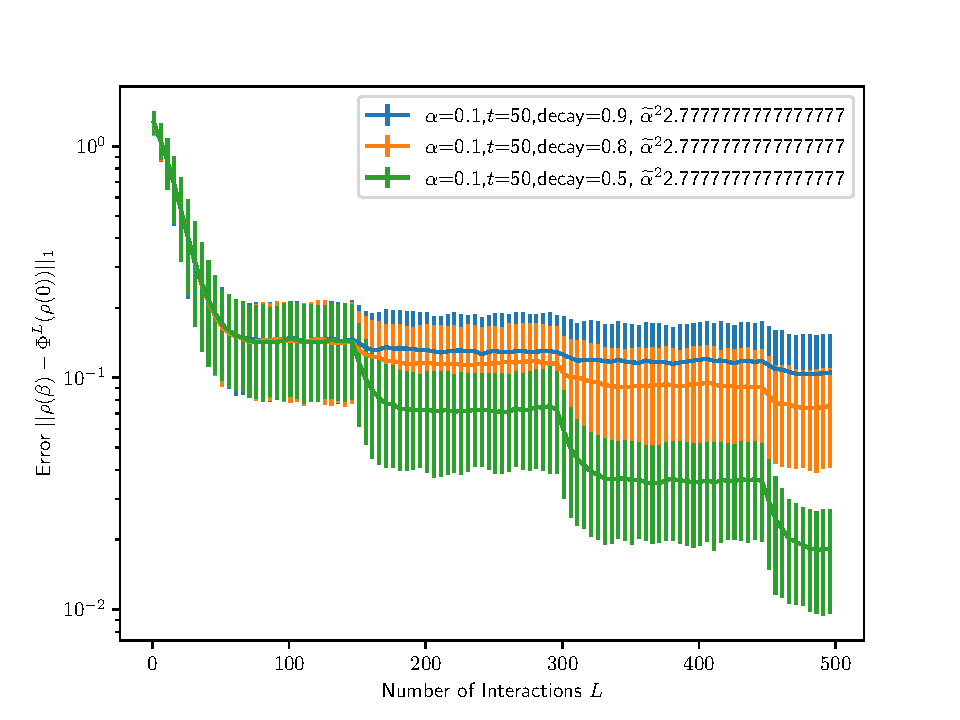
\includegraphics[width=\textwidth]{numerics/data/error_vs_interaction_fixed_time_2.pdf}     
%         \caption{Varying $\alpha$ for a fixed $t$.}
%     \end{subfigure}
%     \begin{subfigure}{0.49\textwidth}
%         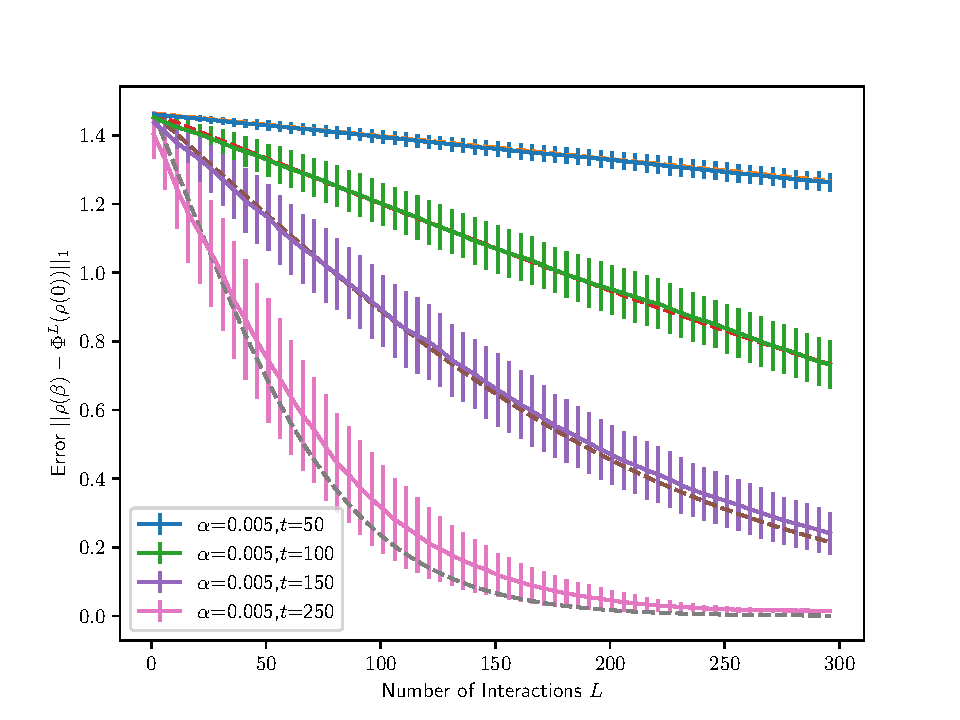
\includegraphics[width=\textwidth]{numerics/data/error_vs_interaction_fixed_time.pdf}    
%         \caption{Varying $t$ for a fixed $\alpha$.}
%     \end{subfigure}
%     \caption{Distance from the thermal state $ \norm{\rho_S(\beta) - \Phi^{\circ L}(\rho_S(0))}_1$ as a function of the number of interactions $L$. The system is a $\dim_S = 4$ truncated harmonic oscillator and $\beta = 8$, so the prepared state has very high overlap with the ground state. We investigate the effects of $\alpha$ and $t$ on the error separately, the top plot keeps $t$ fixed and the bottom keeps $\alpha$ fixed. In both we see that increasing $\alpha$ or $t$ leads to faster convergences. The downside to the faster convergence is a larger deviation from the Markov chain behavior, which is shown in dashed lines for each parameter setting. This could be an issue for very accurate state preparations as $\epsilon \to 0$.}
%     \label{fig:sho_error_vs_interactions}
% \end{figure}




% Now that we have numerically verified the validity of our channel as a thermalizing channel as well as the $\alpha$ and $t$ behavior of our Markov chain, we turn our attention to the total simulation time as a function of $\beta$. This is important as our runtime results for the single qubit are independent of $\beta$ and the only runtime results we have for the harmonic oscillator is for the ground state $\beta \to \infty$. Our numeric results are contained in Figure \ref{fig:sho_total_time_vs_beta}. The method we used is to start our simulation at $\rho = \frac{\identity}{\dim_S}$, as we need a state that commutes with $H_S$ and is easy to prepare. We then find the smallest number of interactions needed for our state to have an average trace distance of less than 0.05, averaged over 100 samples, using values of $\alpha$ and $t$ found by trial and error. We find that even for systems as small as $\dim_S = 4$ there is a nontrivial dependence of the runtime on $\beta$. The total simulation time increases with $\beta$, as one would initially expect, until it reaches a peak and then decreases, indicating colder temperatures can converge \emph{quicker} than warmer temperatures when starting from an infinite temperature initial state. This bump becomes noticeably more pronounced as the dimension increases, see Figure \ref{fig:sho_total_time_vs_beta}. Our explanation for this phenomena is a temperature dependence of the Markov chain spectral gap that is different than the temperature dependence of the distance between the starting state and the thermal state. 


% We first demonstrate the thermalization runtime for the truncated harmonic oscillator, however this time we characterize the runtime needed to thermalize as a function of our knowledge of the spectrum. To parametrize this, as we simulate our repeated interactions channel we sample the environment gaps $\gamma$ from a mixture distribution of Gaussians centered around each eigenvalue difference with a width of $\sigma$. As we vary $\sigma$ from 0 to the maximum eigenvalue difference in the Hamiltonian, we are effectively interpolating our $\gamma$ sampler from perfectly sampling the eigenvalue differences to sampling complete noise. The results in Figure \ref{fig:sho_with_noise} are promising, although we see that having no noise added to the system results in a roughly 10x lower runtime than the completely noisy $\gamma$ samples, the runtime does have a fairly stable plateau. This indicates that the algorithm should work fairly consistently without any knowledge whatsoever of the eigenvalue gaps $\Delta$.

% \begin{figure}
%     \centering
%     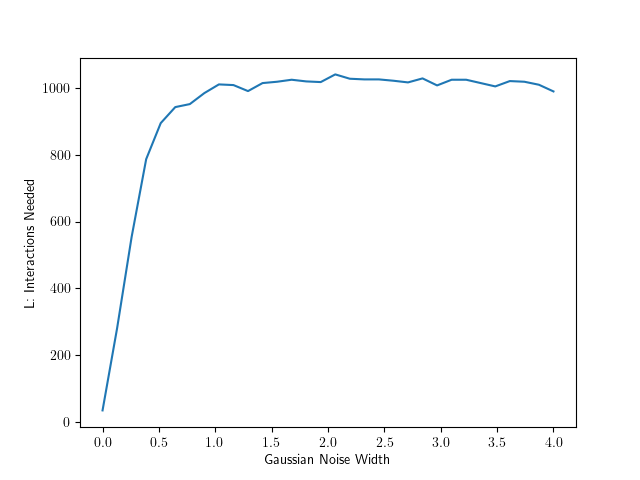
\includegraphics[width=0.5\linewidth]{numerics/data/sho_with_noise_1.png}
%     \caption{Number of interactions needed to reach a trace distance of $0.1$ away from the thermal state with $\beta = 1.0$, for a dimension 5 truncated harmonic oscillator, by sampling from the exact spectrum of the hamiltonian with the amount of added noise indicated by the x-axis. The rightmost limit of the plot is equal to the ``spectral diameter", or the largest eigenvalue minus the smallest. We can see a fairly rapid growth with added noise followed by a fairly stable plateau, indicating that even with minimal to zero knowledge of the spectrum reliable approximation to the thermal state can be prepared. }
%     \label{fig:sho_with_noise}
% \end{figure}


\end{document}